% -*- Mode:TeX -*-
%\documentclass[12pt,twoside,leftblank]{style/mitthesis} 
% ! remove draft mode for the final version 
% \documentclass[11pt,twoside,draft]{style/mitthesis}
\documentclass[11pt,twoside]{style/mitthesis}
% ! remove draft mode for the final version 

\usepackage{style/lgrind}
\usepackage{cmap}
\usepackage[T1]{fontenc}
% \usepackage{times}
\usepackage{adjustbox}
\usepackage{rotating}
% for Verbatim font size
\usepackage{fancyvrb}
\usepackage{subcaption}
\usepackage{enumitem}
% tables 
\usepackage{multirow}
\usepackage{longtable}
\usepackage{lscape}

\newenvironment{rotatepage}%
    {\clearpage\pagebreak[4]\global\pdfpageattr\expandafter{\the\pdfpageattr/Rotate 90}}%
    {\clearpage\pagebreak[4]\global\pdfpageattr\expandafter{\the\pdfpageattr/Rotate 0}}%

% color tables 
\usepackage[table,xcdraw]{xcolor}
% tilde
\usepackage{textcomp}
% math 
\usepackage{amsmath, bm, amsfonts}
\newcommand\inlineeqno{\stepcounter{equation}\ (\theequation)}


% ! remove draft mode for the final version
% \usepackage{background}
% \backgroundsetup{
%   position=current page.east,
%   angle=-90,
%   nodeanchor=east,
%   vshift=-5mm,
%   opacity=1,
%   scale=2,
%   contents={Draft 4 - \today}
% }

\RequirePackage[hyphens]{url}
% link colors 
\PassOptionsToPackage{hyphens}{url}\usepackage{hyperref}
\hypersetup{
    colorlinks   = true,
    urlcolor     = blue,    % Colour for external hyperlinks
  linkcolor    = blue,    % Colour of internal links
  citecolor    = blue
}
\pagestyle{plain}
\def\all{all}
\ifx\files\all \typeout{Including all files.} \else
% prevent replacing of objects
\usepackage{placeins}

%%%%%%%%%%%%%%%%%%%%%%%%%%%%%%%%%%%%
\begin{document}

% Hides the chapter number 
\makeatletter
\renewcommand{\thesection}{%
    \ifnum\c@chapter<1 \@arabic\c@section
    \else \thechapter.\@arabic\c@section
    \fi
}
\makeatother

% REMOVES FIGURES SECTION NUM
\makeatletter
\renewcommand*{\thetable}{\arabic{table}}
\renewcommand*{\thefigure}{\arabic{figure}}
\let\c@table\c@figure
\makeatother
%%%%%%%%%%%%%%%%%%%%%%%%%%%%%%%%%%%%
\title{%
    \Huge CityScope\\
    \Large {
        An Urban modeling and Simulation Platform
    }
}
\author{Ariel Noyman}
\prevdegrees{
    B.Arch, Bezalel Academy of Arts and Design, Jerusalem
    \\
    S.M., Massachusetts Institute of Technology
}
\department{Program in Media Arts and Sciences,\\ School of Architecture and Planning}
\degree{Doctor of Philosophy in Media Arts and Sciences}
\degreemonth{May 13\textsuperscript{th},}
\degreeyear{2022}
\thesisdate{May 13\textsuperscript{th}, '22}
\supervisor{Kent Larson}{Director, City Science Group}
\chairman{Kent Larson}{Director, City Science Group}
\maketitle
\setcounter{savepage}{\thepage}
\setcounter{secnumdepth}{5}
\setcounter{tocdepth}{5}
%%%%%%%%%%%%%%%%%%%%%%%%%%%%%%%%%%%%
% \cleardoublepage
%%%%%%%%%%%%%%%%%%%%%%%%%%%%%%%%%%%%
\begin{abstractpage}
    {Current mass-urbanization trends create vast opportunities and new challenges to cities worldwide. Migration and immigration, climate change, technological disruptions, inequality, affordability, and most recently, global health concerns, are only some of the questions urban decision-makers are facing today. As these challenges grow, traditional urban processes are rendered insufficient: Slow planning processes lag behind rapidly expanding cities, static regulations struggle with volatile economies, and technological disruptions outpace legacy planning mechanisms.}

{In this dissertation I explore an emerging model, in which novel technologies and human-centric methods are coupled to create a \textit{new urban process}. This model marries a systematic, scalable, evidence-based and data-driven decision-making, with a comprehensive, long-term, and community driven participatory process. I explore this \textit{new urban process} through the design, development and deployment of CityScope: a human-centered, urban modeling, simulation and decision-making platform, on the intersection of urban technology and social discourse.}

{This dissertation examines past, current, and future CityScope instances through four perspectives: \textbf{Insight}: CityScope as an urban observatory, using advanced methods in urban and spatial analytics, focusing on high-resolution, geo-located urban-dynamics data.
\textbf{Transformation}: CityScope as an urban simulator for iterative design processes, and a dynamic system for decision-making.
\textbf{Prediction}: Using CityScope to support urban modelling in data-intensive and data-less environments, through methods of urban forecasting, modelling, and simulation.
\textbf{Consensus}: Enabling multi-stakeholder decision-making, consensus and policy processes. Using CityScope to facilitate collaborative and decentralized urban decision-making.} 

{Finally, I report on a series of lab experiments and worldwide deployments of the CityScope platform, and describe how it supported, enhanced, and even replaced traditional urban decision-making, affecting both the urban process as well as its outcomes.}
\end{abstractpage}
%%%%%%%%%%%%%%%%%%%%%%%%%%%%%%%%%%%%
\begin{titlepage}
    \begin{large}
        {\huge\textbf{CityScope}\bigskip}
        \\\textbf{An Urban Modeling and Simulation Platform}
        \\\bigskip
        by\\\bigskip
        Ariel Noyman

        \signature{Thesis Advisor}
        {
            \textbf{Kent Larson}
            \\
            Director, City Science Group,
            MIT Media Arts and Sciences
        }

        \signature{Thesis Reader}
        {
            \textbf{Eran Ben Joseph}
            \\
            Class of 1922 Professor of Landscape Architecture and Urban-planning,
            MIT Department of Urban Studies and Planning
        }

        \signature{Thesis Reader}
        {
            \textbf{Esteban Moro}
            \\
            Associate professor at the Universidad Carlos III de Madrid (Spain),
            Visiting Professor, Media Lab, Massachusetts Institute of Technology
        }
    \end{large}
\end{titlepage}



%%%%%%%%%%%%%%%%%%%%%%%%%%%%%%%%%%%%
\begin{commiteepage}
    %%%%%%%%%%%%%%%%%%%%%%%%%%%%%%%%%%%%%%%%%%%%%%%%%%%%%%%%%%%%%%%%%%%%%%%%%%%%%%%%%%%%%%

\subsection*{Kent Larson} 

{Director, City Science Group, Media Lab}
{Massachusetts Institute of Technology}
\subsection*{Biography}

{Kent Larson directs the City Science group at the MIT Media Lab. His research focuses on developing urban interventions that enable more entrepreneurial, livable, high-performance districts in cities. To that end, his projects include advanced simulation and augmented reality for urban design, transformable micro-housing for millennial, mobility-on-demand systems that create alternatives to private automobiles, and Urban Living Lab deployments in Hamburg, Andorra, Taipei, and Boston. Larson and researchers from his group received the “10-Year Impact Award” from UbiComp 2014. This is a “test of time” award for work that, with the benefit of hindsight, has had the greatest impact over the previous decade. Larson practiced architecture for 15 years in New York City, with design work published in Architectural Record, Progressive Architecture, Global Architecture, The New York Times, A+U, and Architectural Digest. The New York Times Review of Books selected his book, Louis I. Kahn: Unbuilt Masterworks (2000) as one of that year’s ten best books in architecture.}

%%%%%%%%%%%%%%%%%%%%%%%%%%%%%%%%%%%%%%%%%%%%%%%%%%%%%%%%%%%%%%%%%%%%%%%%%%%%%%%%%%%%%%%%%%%%%%%%%%%%%%%%%%%%%%%%%%%%%%%%%%%%%%%%%%%%%%%%%%%%%%%%%%%%%%%%%%%%%%%%%%%%%%%%%%


\subsection*{Prof. Eran Ben Joseph}

{Class of 1922 Professor of Landscape Architecture and Urban Planning, head of the Department of Urban Studies and Planning at MIT from 2013 to 2020}
% 
\subsection*{Biography}
{Eran Ben-Joseph is the Class of 1922 Professor of Landscape Architecture and Urban Planning in the Department of Urban Studies and Planning at the Massachusetts Institute of Technology. Eran served as Head of the Department of Urban Studies and Planning at MIT from 2013 to 2020. His research and teaching areas include urban and physical design, standards and regulations, sustainable site planning technologies and urban retrofitting. He authored and co-authored the books: Streets and the Shaping of Towns and Cities, Regulating Place: Standards and the Shaping of Urban America, The Code of the City, RENEW Town and ReThinking a Lot. Eran worked as a city planner, urban designer and landscape architect in Europe, Asia, the Middle East and the United States on projects including new towns and residential developments, streetscapes, stream restorations, and parks and recreation planning. He has led national and international multi-disciplinary projects in Singapore, Barcelona, Santiago, Tokyo and Washington DC among other places. Eran holds degrees from the University of California at Berkeley and Chiba National University of Japan. Current Research: Urban Form and Health, Urban Form and the Aging Population, Urban Form and Ecological Models of Development, Urban Form and Manufacturing.}

%%%%%%%%%%%%%%%%%%%%%%%%%%%%%%%%%%%%%%%%%%%%%%%%%%%%%%%%%%%%%%%%%%%%%%%%%%%%%%%%%%%%%%%%%%%%%%%%%%%%%%%%%%%%%%%%%%%%%%%%%%%%%%%%%%%%%%%%%%%%%%%%%%%%%%%%%%%%%%%%%%%%%%%%%%


\subsection*{Prof. Esteban Moro}

{Associate professor at the Universidad Carlos III de Madrid (Spain). Visiting Professor, Media Lab, Massachusetts Institute of Technology}
% 
\subsection*{Biography}
% 
{Prof. Esteban Moro is a visiting professor at the MIT Media Lab, an associate professor at the Universidad Carlos III de Madrid (Spain) and a member of the Joint Institute UC3M-Santander on Financial Big Data. Prof. Moro serve as a consultant for many public and private institutions and have held previous positions at the University of Oxford, Institute of Knowledge Engineering (Spain), and Instituto Mixto de Ciencias Matemáticas (Spain).Moro research is on applied mathematics, financial mathematics, viral marketing, and social networks. He received the "Shared University Award" from IBM in 2007 for modeling the spread of information in social networks and application to viral marketing and the Research Excellence Awards in 2013 and 2015 from the Carlos III University of Madrid. His recent work has been covered by many media outlets, including articles and interviews in El Pais, Muy Interesante, The Atlantic, The Washington Post, and The Wall Street Journal.}

\end{commiteepage}
%%%%%%%%%%%%%%%%%%%%%%%%%%%%%%%%%%%%
\section*{Acknowledgments}
 {
  I first joined Kent Larson's group as a student in his `Beyond Smart Cities' workshop in 2014. At the time, I did not know what Smart Cities meant, why we need to move \textit{beyond} them, and what \textit{science} had to do with all of that. Within a couple of weeks, I knew I'll be shifting my Master program into Kent's group. A few months later, Kent would offer me to lead the founding of a new City Science lab in Hamburg; the rest of the story is laid out in this thesis.
  \newline
  I cannot be grateful enough for Kent's generosity, kindness, and his belief in people. I learned many things from Kent, but most importantly is that great things come from the least expected people, if you only create the conditions for them to do so. I am grateful for his mentoring, guidance, and friendship during these years.
  \newline
  I wish to thank my committee. Prof. Eran Ben-Joseph has been a key supporter, motivator, and advisor during my entire journey at MIT. His work on the intersection of technology, urbanism, law, and design, was a major inspiration to both my master's thesis and this dissertation.
  I have learned a lot from countless interactions and conversations with Prof. Esteban Moro. Coming from pure theoretical physics into the unholiness of the built environment, Esteban showed me the beauty of applying sophisticated science to the most pedestrian challenges.
  \newline
  Many mentors have been instrumental to my work and growth.
  \newline
  I thank my many friends, collaborators, and colleagues at the City Science Network worldwide, for their wisdom, hospitality, and shared passion for better cities. Building a vibrant network of City Science Labs, from Southeast Asia to South America, has been one the best experiences of my tenure at MIT. Specifically, I'd like to thank Prof. Gesa Zimmer and Prof. Jörg Noennig from the HafenCity University in Hamburg, for allowing me to be part of the founding team of the CityScienceLab. Since 2015, the entire CityScienceLab team has been a tremendous force in my journey, especially (in alphabetical order) Andre, Frank, Holger, Imanuel, Jan Ba., Jan Be., Jesús, Katrin, Nina, Sarah, Till, and Tobi.
  \newline
  All of the projects mentioned in this thesis were created by the wonderful members of the MIT City Science group, alongside collaborators from the City Science Network, and with the help of many external partners\footnote{The first version of cityIO was create by Nikita Samsonov (MIT EECS) in 2015. Since then, cityIO is maintained by Yasushi Sakai (MIT Media Lab). CityScopeAR was conceived with the help of Nikita Samsonov (MIT EECS) and Dalma Foldesi (MIT SA+P). Yuke Zheng (Harvard University) made significant contributions to the development of CityScopeJS. For individual contributor information, please see references in Section \eqref{sec:publications-projects-deployments}.}. I would like to thanks the core members of the CityScope team (in an alphabetical order): Arnaud, Cris, Luis, Markus, Ronan, Ryan, and Yasushi; None of the work presented here would have been possible without you. Arnaud and Luis: Thank you for being my right and left hand, interchangeably. Ronan: Thank you for leading my in mystical ways of Data Science; May your models always fit. Countless other contributes have made CityScope better each day: from thousands of CityScope users worldwide, through anonymized open-source contributions, to makeshift CityScope creators, they all share the same hope for better cities. Thank you all.

  \bigskip
  \begin{center}
      $\sim$
  \end{center}
  \bigskip

  I am grateful for my family. My parents, Shlomit and Moshe, brothers Johnathan and Gilad, and the entire family, for their unconditional love and support during these years. I would like to commemorate my late grandmother Bina, who's wisdom and wonder motivated my journey.

  \bigskip

  To Arad and Ori, for reminding me of what's important. May we leave better cities for your future.

  \bigskip
  To Roni, who took me out my comfort zone, and created comfort whenever I needed it. None of this would have been possible without you.
 }
%%%%%%%%%%%%%%%%%%%%%%%%%%%%%%%%%%%%
\newpage
%%%%%%%%%%%%%%%%%%%%%%%%%%%%%%%%%%%%
\tableofcontents
%%%%%%%%%%%%%%%%%%%%%%%%%%%%%%%%%%%%
\clearpage
%%%%%%%%%%%%%%%%%%%%%%%%%%%%%%%%%%%%
\pagestyle{plain}
%%%%%%%%%%%%%%%%%%%%%%%%%%%%%%%%%%%%

\begin{figure}[!htb]
    \begin{center}
        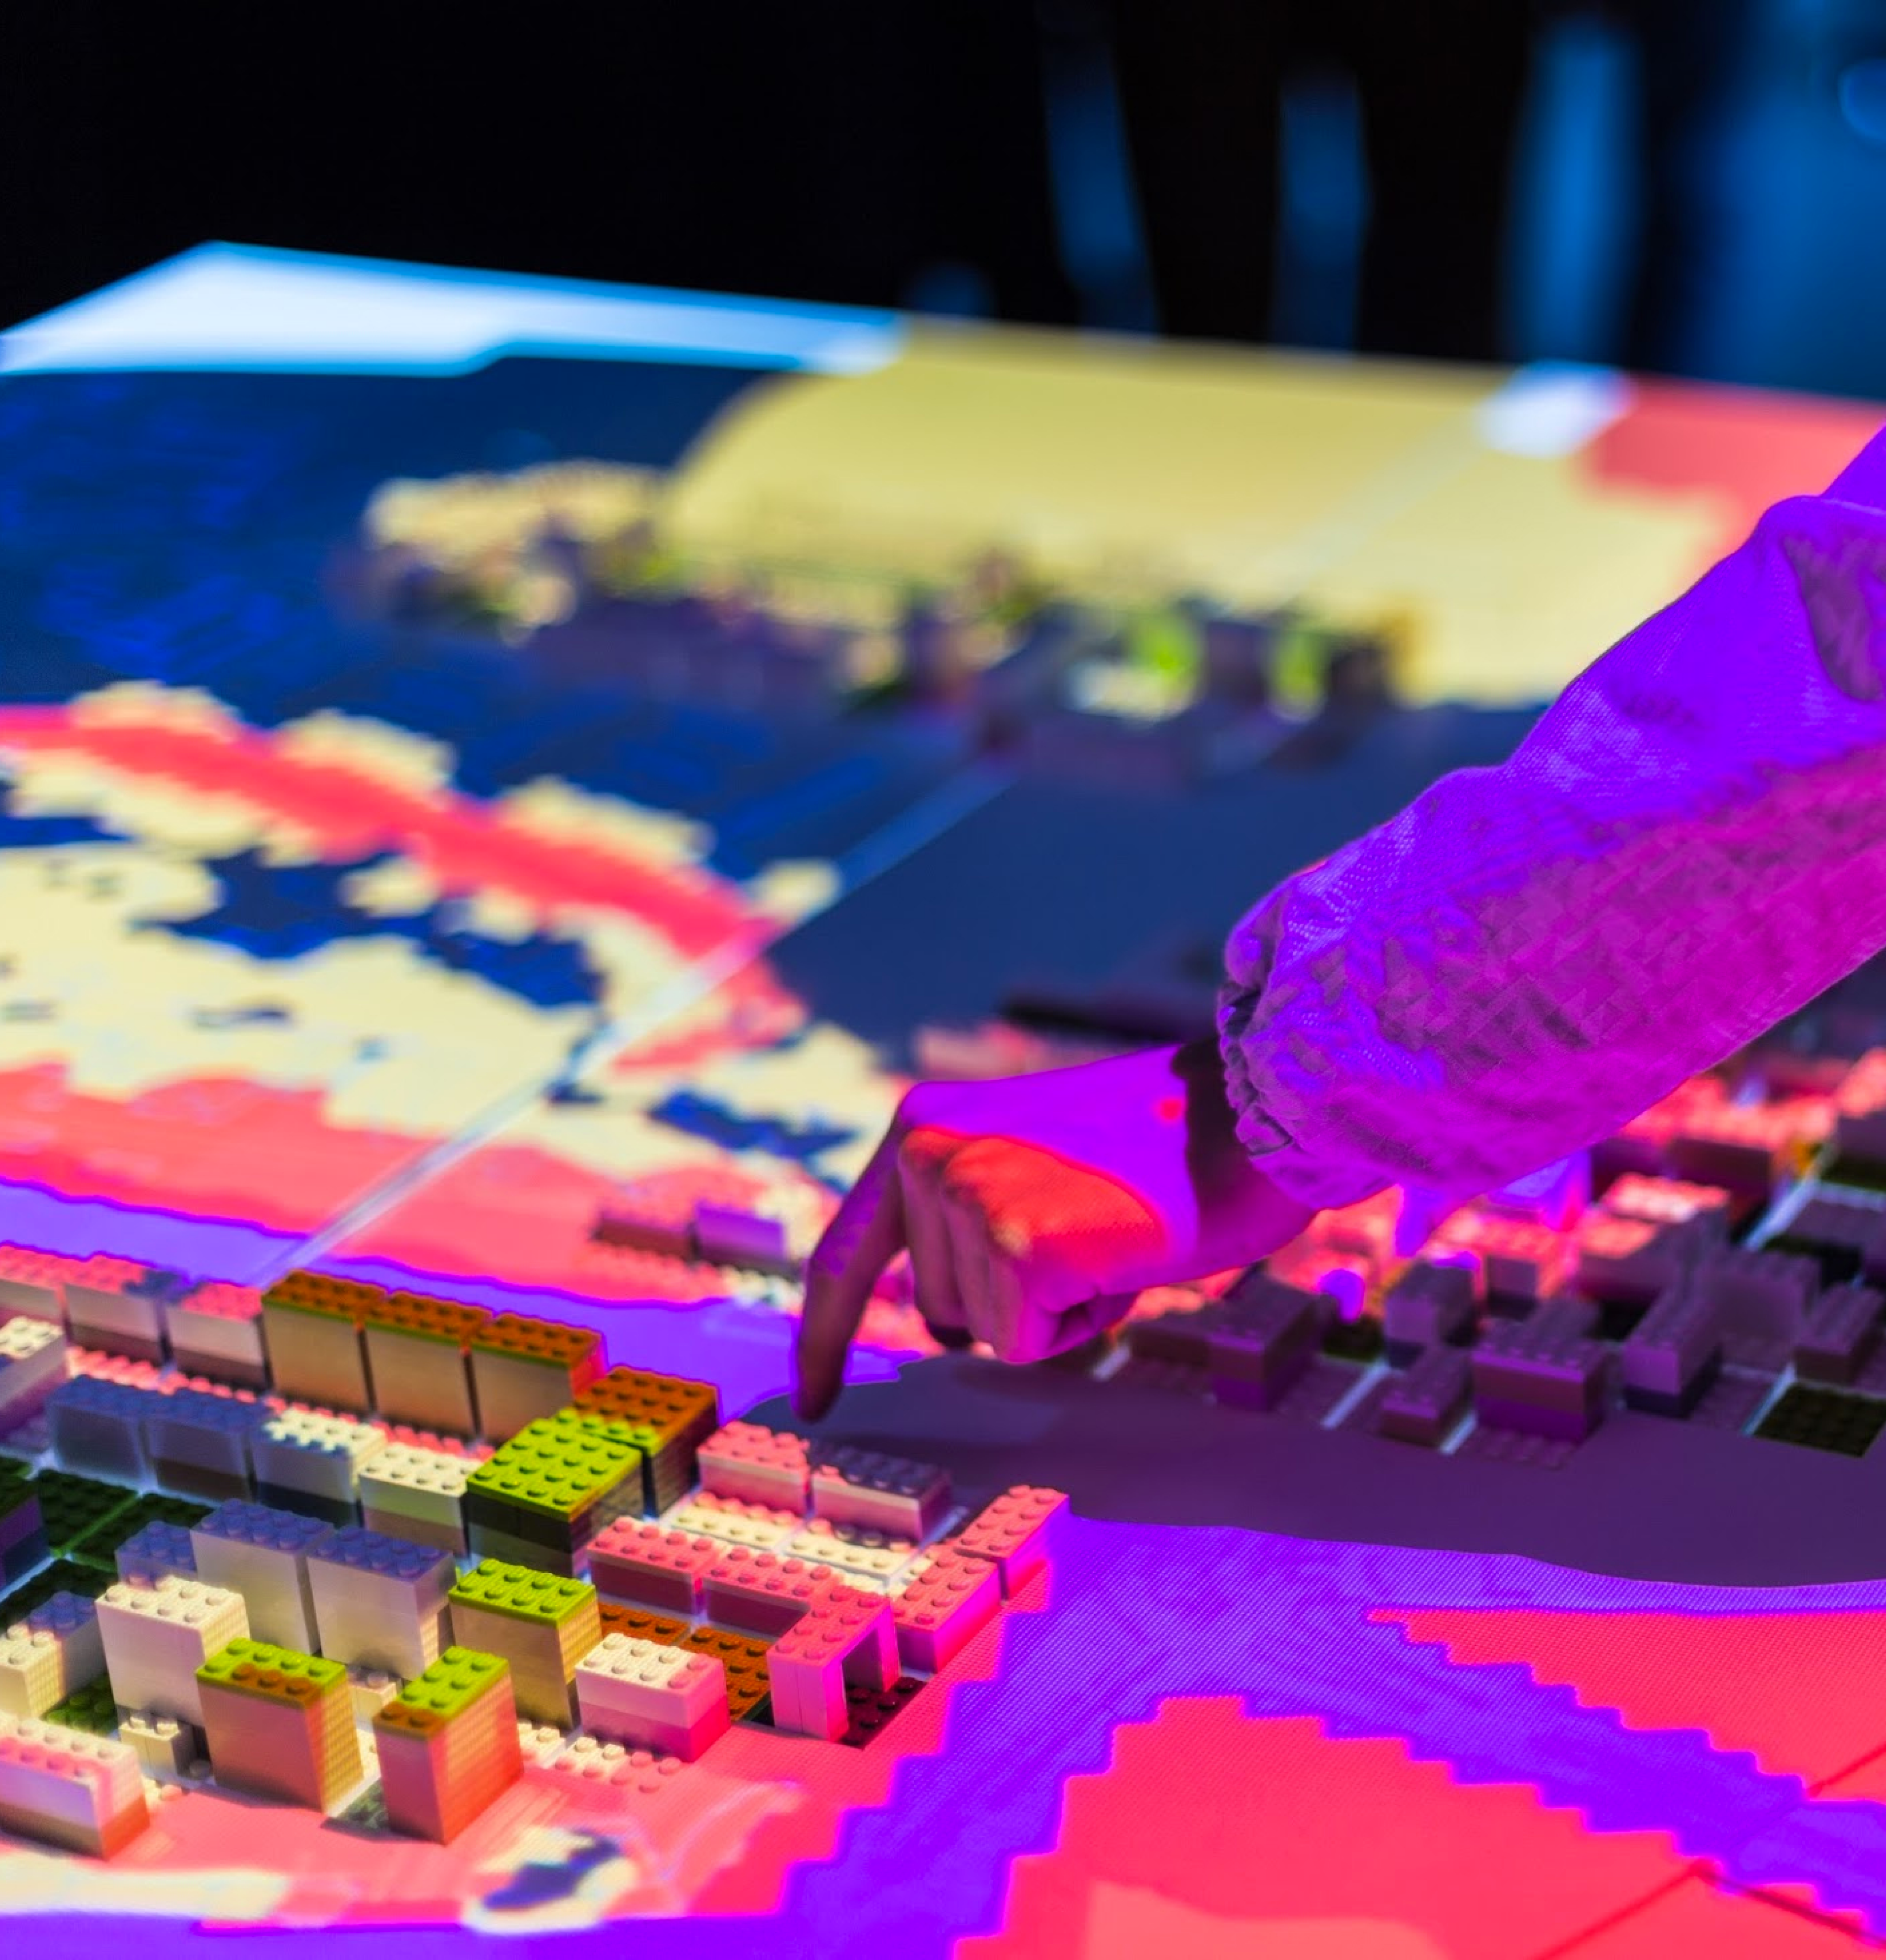
\includegraphics[width=1\textwidth]{chapters/main/figures/hcu_workshop.png}
    \end{center}
    \caption{
        A researcher interacting with the CityScope platform at the HafenCity University in Hamburg, Germany (Nov, `16). This was the final phase of a week-long CityScope workshop, in which researchers develop their own CityScope analysis modules and use them as part of an interactive planning discussion.
    }
    \label{fig:hcu_workshop}
\end{figure}
\newpage

%%%%%%%%%%%%%%%%%%%%%%%%%%%%%%%%%%%%
\include{chapters/introduction/introduction}
%%%%%%%%%%%%%%%%%%%%%%%%%%%%%%%%%%%%


\chapter{Insight\label{ch:insight}}

\section{Introduction}
 {

  Prior to any change to the built environment, is the full understanding and evaluation of the current state of the city. Gaining meaningful insights can highlight places, policies, or behaviors in need for transformation, so that decision-makers can better focus their resources and efforts. As a complex systems of systems \cite{Batty2009}, the many different layers of information in the city are challenging to comprehend. Narrowing the spectrum of possible observations, through methodical data collection, accurate analysis, and clear representation, is a critical step towards a productive planning discourse \cite{banerjee2011companion}. This chapter discusses how CityScope is used to expose the current state of the city, focusing on data aggregation, analysis, and representation.


  \subsection{From Static Data to Urban Dynamics}

  {
      In recent decades, many data-driven methodologies emerged to provide empirical assessments of urban performance \cite{Inostroza2015, hillier1987ideas}. In the 1970's, `Space Syntax' was proposed as a set of analytical tools to interpret the \textit{``ordering of space into relational systems''} \cite{Hillier1993}, using quantitative analysis to infer the performance of spatial networks. At the time, data accuracy and geometric-spatial limitations confined the results to generalized outputs \cite{herold2005role}. Today, the abundance of urban data and the advancement of spatial analytics greatly improve the resolution and accuracy of these evaluations \cite{Batty2000}. Nevertheless, urban performance cannot be solely interpreted by analyzing urban-form: the quality of a place is a joint artifact of physical places and the society which occupies them \cite{lynch1984good}. To associate form with behavior, Lynch proposed \textit{``Performance Dimensions''}: a set of spatial and experiential urban features, bridging the gap between form and usage. Along the same lines, Gehl suggested metrics to reflect the social impacts of a public space and the quality of life of its users \cite{gehl2013study}. Today, with the growing ubiquity of tracking devices and slew of behavioral data, it is possible to analyze the `real-time city', as a useful design and planning apparatus \cite{ Ratti2006, Kitchin2014, Batty2013}.
  }

  \subsection{Urban Dynamics: Mobility and Behavior}\label{subsec:andorra-data-observatory-mobility}

  {
      The growth of Location Based Services (LBS) motivated the research of the city's `beating pulse' \cite{Becker2011}. In recent decades, mobile devices became the major way to observe human dynamics, behavioral patterns, mobility, large public events, and emergencies \cite{Blondel2015, Calabrese2014, Reades2007, gonzalez2008understanding, Deville2014, Berlingerio2013}. Other location sensing technologies, such as GPS, radio frequency identification, cameras, or activity sensors, are all limited in their spatial capacity, the need for active user-interaction (`opt-in'), and complexity of data extraction.
      \newline
      Studies in Belgium, UK, Ivory Coast, and Spain showed correlations between the spatial form of cities, the distribution of their activity `hot-spots', and the degree of interaction between different cellular users \cite{Blondel2015, Louail2014}. Similarly, spatial-temporal regularity within behavioral trajectories was found in mobile phone users, suggesting that individuals can be clustered into different groups based on their behavioral patterns \cite{Song2010}. Others have used LBS to characterize individual trajectories across the city, showing collective behavior and `flocking' patterns \cite{Ratti2006, DecodingtheCity}. Despite the promise of location data for urban analytics, challenges still exist in data accuracy, temporal resolution, and bias.
  }

  \subsection{Limitations of LBS}

  {
      In the past, LBS limitations in data quantity, reliability, and accuracy have forced spatial generalization and limited outcomes \cite{candia2008uncovering}. In many cases, Call Detail Records (CDR) data were the prevailing LBS in use \cite{jiang2017activity}. CDR provide usage history, cell tower ID, and approximate coverage region of each base-station, which together are used to estimate the location-time of users. However, CDRs suffer from low temporal and spatial resolution, since location information is only provided at the cell tower level and updates are only received when the device is in use, such as during calls or text \cite{Calabrese2014}. Moreover, studies have shown that CDRs tend to underestimate the total travel distance and movement of users \cite{VonMorner2017}. The low accuracy and the event-triggered nature of CDR might be acceptable for mobility, sensing large events, or emergency analysis, but biases appear when attempting analyzing individual trajectories \cite{Zhao2016}. Higher resolution data could be obtained through signal strength aggregation of multiple cell towers (RSS), using geolocation techniques such as received signal strength and triangulation \cite{blondel2015survey}. More accurate telecom data, such as Radio Network Controller (RNC) data, can potentially help overcome these biases and better present individual patterns. In other cases, superimposing several data sources, such as LBS, GPS, census, and land-use all together, can improve the overall resolution of models and increase their accuracy \cite{Blondel2015}.
  }
  \newline
  In summary, assessing mobility and behavior is still a challenge which require a large number of data sources and different analysis techniques. The following section details CityScope insight case-studies, ranging from static observations, such as land-use and population density, to urban-dynamics observations, such as movement, behavior, and interaction. It concludes with a discussion on the limitations, potential, and future of urban insights.
 }

%%%%%%%%%%%%%%%%%%%%%%%%%%%%%%%%%%%%%%%%%%%%%%%%%

\section{CityScope Insights: Case Studies}

 {
  The following are CityScope \textit{insight} projects, focusing on spatial, temporal, and behavioral observations of the city. The \textbf{Urban Data Observatory} \cite{Hadhrawi2016} (2013-2016) visualized various pre-computed insight layers (such as urban form, mobility systems, solar emission, or wind regime) of the Kendall Square area in Cambridge, MA (see Section \eqref{sec:urbanobservatory}). In later projects, data analysis and visualization was used to inform the research question and establish metrics for interventions. In \textbf{CityScope Andorra} (2015-2016), LBS data were used to extract high-resolution mobility trajectories, to interpret how people move, by which modes of transportation, their daily routines, as well as their impact on congregation, `hot-spots', and points of interest (see Section \eqref{sec:andorra-data-observatory-andorra}). These insights can support urban-planning, traffic and energy optimization, tourism, large-event management, and more. As the following Chapter details, these insights are used as baseline for CityScope transformation processes.
 }

%%%%%%%%%%%%%%%%%%%%%%%%%%%%%%%%%%%%%%%%%%%%%%%%%

\section{The Urban Observatory: CityScope Kendall Square}

 {
  One of the first instances of CityScope was the `Urban Observatory' \cite{Hadhrawi2016}. It was firstly constructed as part of a City Science Workshop by MIT students in 2013, to communicate and visualize corresponding spatial layers. The Urban Observatory was a dynamic visualization tool, designed to replace static models of cities, and provide expert and non-experts with a decision-support system. It employed a set of pre-defined spatial analytics layers, an array of a video projection mapping, and 3D physical models. The Urban Observatory was used as a `sandbox' platform and research context, on which observations and developed proposals for new urban-design for a site in Cambridge, MA were displayed.

  \begin{figure}[h]
      \begin{center}
          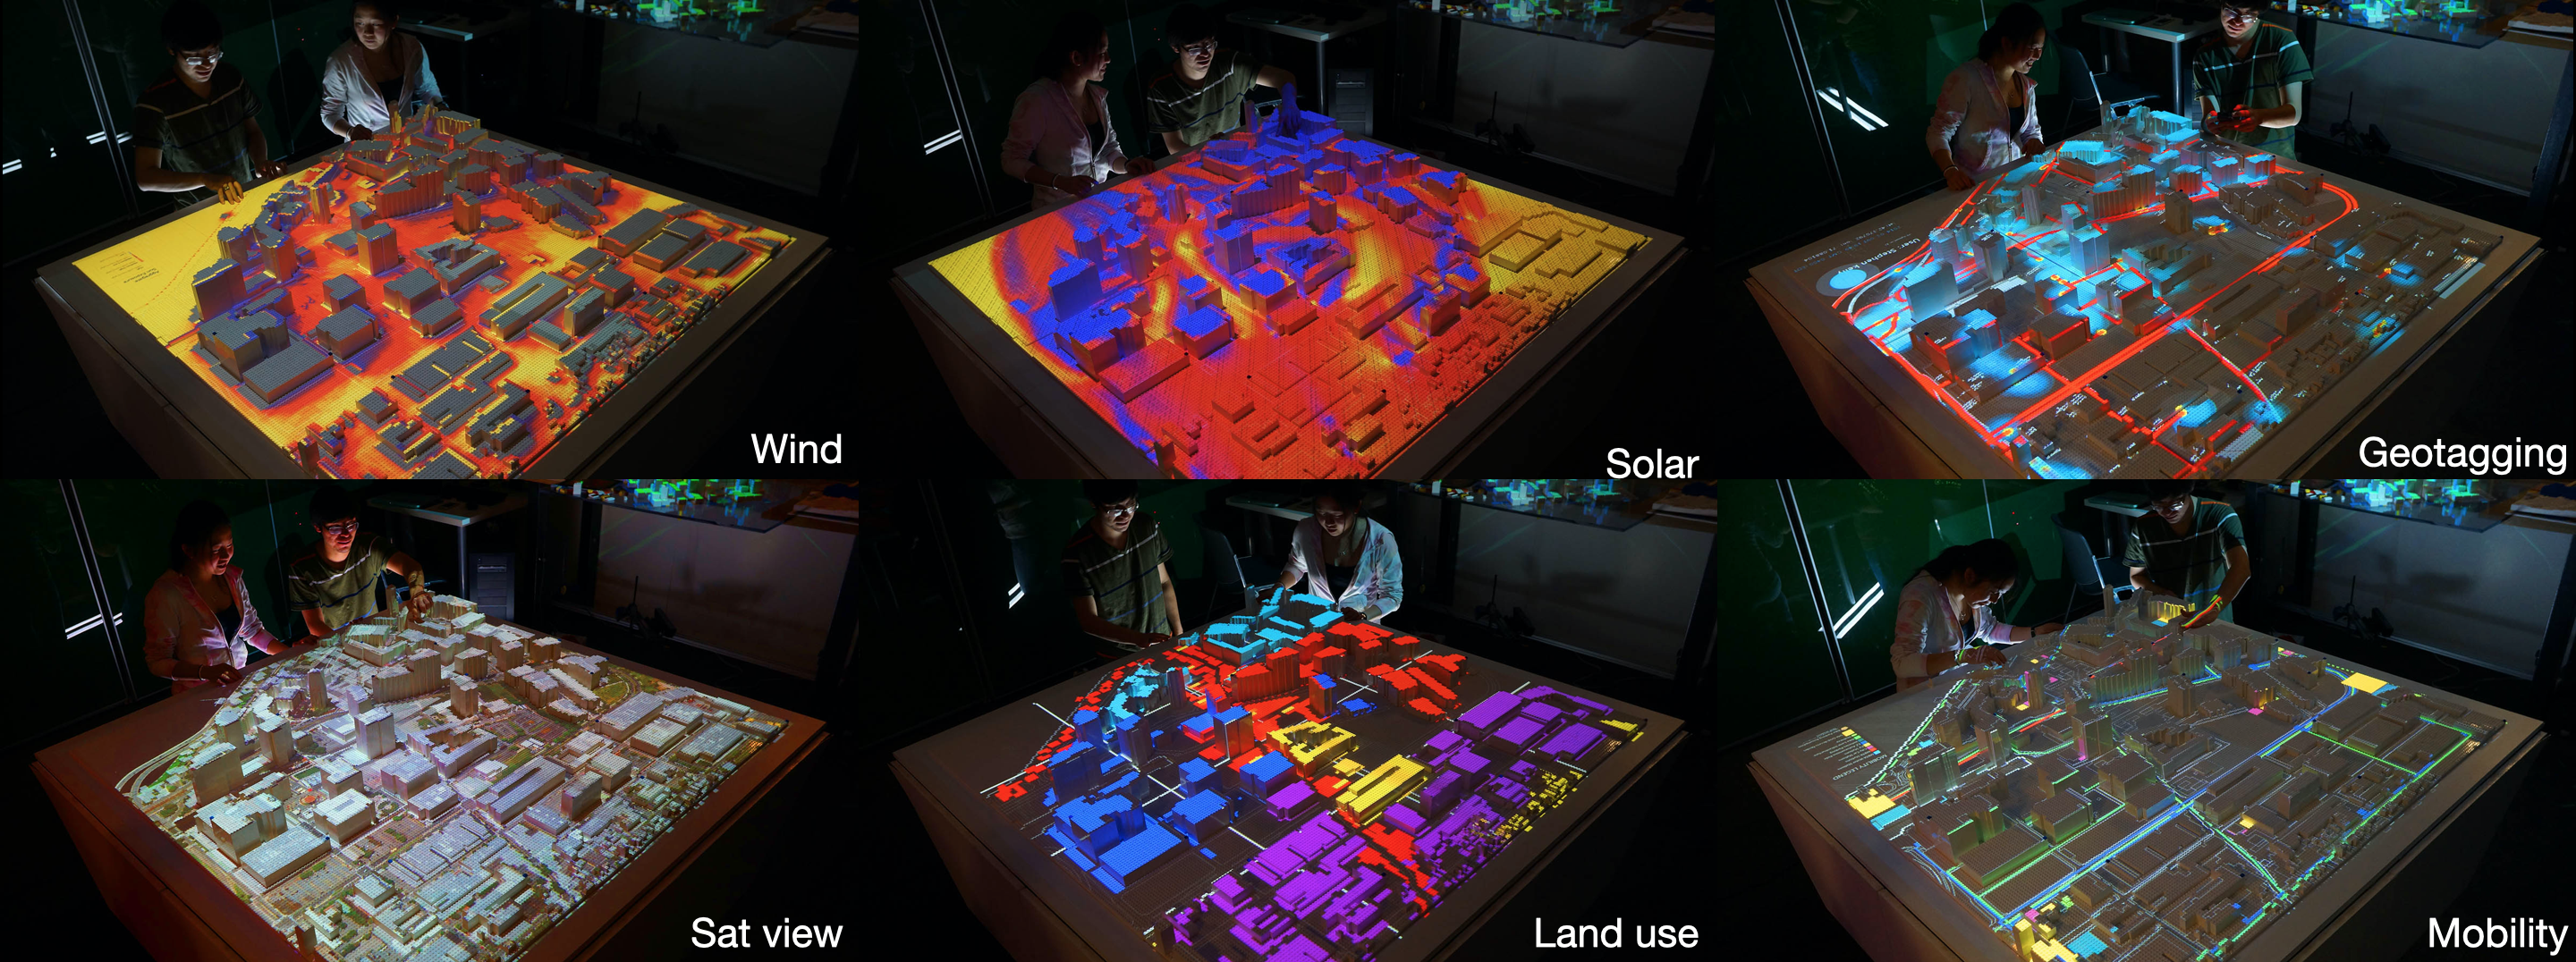
\includegraphics[width=1\textwidth]{chapters/insight/observatory/figures/urban_obs.png}
      \end{center}
      \caption{The Urban Observatory. Different layers of precomputed urban analysis projected onto a 3D model of the Kendall Sq. area in Cambridge, MA.}
      \label{fig:urban_obs}
  \end{figure}

  \subsection{System Design}
  {
      The Urban Observatory comprised of physical components, computer hardware, and custom display software, detailed bellow.

      \subsubsection{Computation}{\label{sec:computational-models}}
      {
          The Urban Observatory was design as an open canvas for displaying different layers of data, such as the formal properties of building designs, land-use, human activity and mobility, vehicular circulation, flows of energy, wind and solar exposure, and more (see Figure \eqref{fig:urban_obs}). These layers were pre-rendered in advance, since the platform was not set to perform spatial analytics or data acquisition in real-time\footnote{In later versions of CityScope, data for similar layers was fetched in real-time, and was rendered dynamically to reflect updated insights or user-interaction. See Chapter \eqref{ch:transformation}}. As part of the students' workshop, architectural, urban-planning, traffic-simulation, and visualization tools were all used to produce these data layers. The projection were projected and aligned to the 3D model using a Processing sketch \cite{reas2007processing}.
      }

      \subsubsection{Hardware}
      {
          The system contained two main elements: (i) a 3D urban model, made out of white LEGO bricks, and (ii) an array of overhang projectors. The physical model was of size $1.7m^2$, which represent a $1km^2$ area of Kendall Square, roughly as the scale of $4m$ for each LEGO stud. For projection, six video projectors were used: two to project the ground and roof planes of a physical model, and one projector for each of the four vertical surface orientations (north, south, east, and west), creating the illusion of 360$^{\circ}$ projection.
      }
  }

  \subsection{Usage}
  {
      The `Urban Observatory' was developed and situated in an active demonstration space at the MIT Media Lab building. Between '13-'16, hundreds of visitors, researchers, and students interacted with the installation; In 2015-2016, the platform was repurposed to support \textit{MAS.S65: The City Science Workshop}, an MIT course that was focused on prototyping new ways to collect and represent urban insights and spatial data. These insights were broad, and ranged from analyzing crime and energy, to vegetation and thermal comfort. Later that year, the 3D models was again repurposed to set as the base line for the CityScope Volpe project (see Section \eqref{sec:cityscope_volpe}).
  }

  \subsection{Discussion}{\label{subsec:observatory_discussion}}

  {
      The Urban Observatory was an early CityScope prototype, which projected pre-defined data layers and urban observations onto a tangible interface. Despite its simplicity, this prototype proven the advantage of merging spatial data and tangible interfaces, as a means to create a new `common ground' for urban discourse. This work also hinted to several features of future CityScope, such as: (i) A Data Warehouse that would store urban data, and spatial analytics algorithms (later to become cityIO, see Section \eqref{subsec:csarch-cityio}); (ii) User Interface, to provide a flexible and intuitive interaction for exploring different urban scenarios (such as CityScope TUI, see Section \eqref{subsec:mocho-volpe}); (iii) Interactive visualizations, to provide dynamic feedback to the users' design iteration (later to become CityScopeJS, see Section \eqref{sec:cityscope_architecture}). Arguably, the Urban Observatory's greatest contribution to the future of CityScope, was the idea of an open-ended urban `sandbox', on which new scenarios could be tested, and user contributions, feedback, and insights, would be collected.
      \newline
      As shown in the following work, later CityScope projects centered around behavioral, social, and economic insights, in order to look beyond the formal and physical aspects of the city.
  }
 }\label{sec:urbanobservatory}
%%%%%%%%%%%%%%%%%%%%%%%%%%%%%%%%%%%%%%%%%%%%%%%%%

\section{Urban Dynamics: CityScope Andorra}\label{sec:andorra-data-observatory-andorra}

{
    In 2014, the Andorran government and the MIT City Science group founded a `living lab' to prototype, deploy, and test urban innovation \cite{SmallEur15:online}. As part of this partnership, the Andorran Government promoted projects related to urban data collection and analysis, and supported this effort by sharing spatial, behavioral, and telecom data. Using these datasets, various research projects were proposed, including the analysis of tourism, mobility, urban-design, energy, environment, and public health \cite{9580719, Grignard:2018:CAM:3237383.3238030, leng2016analysis, noyman_inpress, doorley2020mpec}. The rest of this Chapter details case-studies that used these datasets for the purpose of gaining urban insights and supporting decision-making processes.
}
%%%%%%%%%%%%%%%%%%%%%%%%%%%%%%%%%%%%%%%%%%%%%%%%%
\section{(i) Andorra Data Observatory}\label{sec:andorra-data-observatory}
{
    As part of the collaboration with the Andorran government, a set of tools to analyze, visualize, and extract insights on large public events were create. This section details a data-visualization platform that (i) models the trajectories of large amount of individuals and visitors in several public gathering in Andorra's major cities, (ii) use Agent Based modeling (ABM) to analyze these patterns, and (iii) extract relevant insights and conclusions from these insights.

    \begin{figure}[h]
        \begin{center}
            \includegraphics[width=1\textwidth]{chapters/insight/and_abm/figures/and_cityscope.jpg}
        \end{center}
        \caption{CityScope Andorra at the City Science Lab in Caldea, Andorra la Vella. Built in 2016, this platform was one of the first to serve as an interactive, real-time tool for urban decision making. Here, a user interacts with a Tangible User Interface to asses the impacts of different interventions in the city center.}
        \label{fig:and_cityscope}
    \end{figure}

    \subsection{Events}
    {
        Andorra has a population of nearly eighty thousand, and hosts more than eight million visitors in a normal year, many of them as tourists\footnote{According to the \textit{Departament d\'Estad\'istica}, Andorra had approximately eight million visitors in 2016: 4.2M Spanish, 3.2M French, and 0.6M from other nationalities.}. The tourism sector accounts for $\sim$80\% of Andorra's GDP and thus large public events are critical for the local economy \cite{CIA}. This work focuses on observing the mobility patterns of both pedestrians and vehicles, as a product of tourists and visitors' attendance at annual events in Andorra. The work focuses on the following events: (i) \textit{Cirque du Soleil: VISION} and (ii) \textit{Le Tour de France}, both took place in 2016.
        \newline
        `Scalada' by \textit{Cirque du Soleil: VISION}, is a series of indoor, summertime shows, taking place between Tuesdays to Saturdays, July 2\textsuperscript{nd} - July 30\textsuperscript{th}, 2016. VISION's venue has a capacity for 5000 people per performance. \textit{Le Tour de France} is an annual multiple stage bicycle race held in France, which occasionally passes through nearby EU countries. In 2016, Andorra hosted \textit{Le Tour de France} Stage 9 in its mountain area (Arcal\'is, Ordino) as well as the departure of Stage 10 in the city center (Escaldes, Escaldes-Engordany).
    }

    \subsection{Data and Method}
    {
        Call Detail Records (CDR) are digital records gathered by the mobile network operator used for billing purposes. Observations are triggered by mobile phones actions such as phone calls, text messages, and cellular data. This source of data is broadly used in the research community, since it contains spatial information, allowing to conduct flow analyses \cite{Blondel2015, ccolak2015analyzing, Ratti2006}. As part of this work, Andorra Telecom shared nearly three years of CDR data (2014-2016)\footnote{In order to comply with privacy policies, all personal identifiers, such as names and mobile phone numbers, were anonymized based on a Secure Hash Algorithm (SHA-512), a one-direction encryption method preventing the retrieval of the information obscured.}. Each entry in the CDR contains unique anonymized caller id, the date and time of the call, call duration, and the id of the Base Transceiver Station tower, as shown in table \eqref{f:CDRSample}. with this data, tower-to-tower origin and destination matrices (OD) for each individual were computed.


        \begin{table}
            \begin{center}
                \begin{tabular}{c|cccc}
                    \hline
                    Anonymized ID & Call Date & Call Time & Duration & towerID \\
                    \hline
                    iAAJKnPAa5    & 20160716  & 09:34:13  & 18       & 2       \\
                    iAAJKnPAa5    & 20160716  & 10:21:43  & 156      & 6       \\
                    iAAJKnPAa5    & 20160716  & 13:02:37  & 38       & 10      \\
                    \hline
                \end{tabular}
                \caption{Sample of a CDR observation}
                \label{f:CDRSample}
            \end{center}
        \end{table}


        \subsubsection{Road Network}
        {
            CDR data provide scarce localizing per given user. The nature of these data dictates simplified tower-to-tower OD matrices that correspond to linear, non geographically accurate vectors. In order to correlate these trajectories to the existing road network, users are constrained to roam along a graph topology \cite{Gonzalez2008}. Roads of different types are set to bound different mobility modes (primary, secondary, residential, or pedestrian). In order to compute a more accurate shortest path, the road network is considered as a weight-directed graph used to constrain the behavior of users. The edge direction represents the directionality of the road; The weight combines the speed limit of the road and the number of user present on that road.
        }

        \subsubsection{POIs and Amenities}
        {
            Given the degree of noise in CDR data, urban amenities, such as restaurants, hotels, and other Points Of Interest, were used to anchor destination points of users. The geolocation of amenities was gathered using several public APIs, such as TripAdvisor and Yelp, as well as the \textit{Andorra Turisme} office.
        }
    }

    \subsection{System Design}
    {
        Processing the LBS dataset, and constraining the agents' movement to the road network and POIs, was done using GAMA, an Agent Based modeling (ABM) software \cite{grignard2013gama} and Processing \cite{reas2007processing}. Using a Tangible User Interface (TUI), users could interact with the simulations, and trigger different visualization layers. The three main classes in the model are an abstraction of the (i) environment (cell towers, roads, and amenities), (ii) mobile agents (people and vehicles), and (iii) interactive grid. The rest of this section details the implementation of the ABM and the visualization of the results on a TUI.

        \begin{figure}[h]
            \begin{center}
                \includegraphics[width=0.4\textwidth]{chapters/insight/and_abm/figures/and_cdr_arch.png}
            \end{center}
            \caption{CityScope Andorra data pipelines and TUI. The ABM is computed from both static (GIS) and dynamic (telecom) datasets. It reacts to changes occurring on auxiliary interfaces (CityScopeAR, CityMatrix) and recompute the simulation in accordance.}
            \label{fig:and_cdr_arch}
        \end{figure}


        \subsubsection{Agent Based Model}
        {
            The ABM uses several datasets to characterize agents' behavior in the city: (i) telecom data, (ii) road network, and (iii) amenities and POIs data.
            \newline
            \textbf{Agents:} The virtual environment (`world') is populated with independent agents, each with an assigned set of variables that influence their behavior whenever changes occurs, either locally or at the surrounding environment. \textbf{State:} The agent's variables are (1) agent's country of residence; (2) origin location: defined using telecom data; (3) preferred destination, generated by predefined or dynamically added urban anchors; (4) distance traveled; (5) speed of movement; and (6) passable network nodes. \textbf{Behavior:} The agent's trajectory is determined by the OD matrix computed from the CDR data. The path is computed by constraining the OD to the local road network. The agent's destination is anchored to the amenity closest to the cell tower coverage where its action was recorded when terminated. The chosen amenity depends on the agent's country of residence and the language affinity of the amenities. Depending on its speed (time difference between origin and destination location), the agent will be considered as a pedestrian (solid circle) or as a vehicle (stroke circle).
            \newline
            Agents can adapt themselves to several dynamic factors: (i) traffic congestion: in case of severe congestion, a pathfinding method is called to recalculate an alternative route. If a road is busy, the agent will recompute a shortest path to its destination in order to avoid that road; and (ii) amenity occupancy: if the amenity assigned as destination is flagged as full, the agent can select another amenity close-by to its prior destination. Once agents reach their destination, they stay there for a few iterations. The number of iterations is defined by the average time spent on those places, retrieved from the different APIs.
        }

        \subsubsection{Visualization}
        {
            The ABM was displayed via three main visual layers: (i) Spatial elements, such as geography, buildings, amenities, cell towers, and roads, (ii) Pedestrian and vehicular movement from the ABM, and (iii) Amenities' popularity and density. Pedestrians were represented by solid circles and vehicles by stroke circles, colored according to their origin country: Orange refers to visitors from Spain, blue for France, and white for other countries\footnote{This classes were suggested by \textit{Departament d'Estad\'itica d'Andorra}, although the telecom data has more detailed classification via the IMSI property}.
            The visual representation of POIs and amenities echos the number of agents currently resting at a given location, indicating the activity level in a place. The large white circle highlights the location where the show was taking place. The simulation concluded that 5,174 visitors attendees at the same time, within a reasonable range of \textit{Andorra Turisme} official tally of 4,540 visitors.
            \newline
            Unlike \textit{Cirque du Soleil}, \textit{Le Tour de France} is an outdoor event in which no ticketing process can help assess attendance. Therefore, an aggregated heatmap representation was used to summarize global activity, and provide geo-located attendance estimates. Figure \eqref{fig:and_cdr_viz} show occupancy levels for \textit{Le Tour de France} during July 12\textsuperscript{th}. The race starting point was at Escaldes-Engordany, shown as the most active area in Figure \eqref{fig:and_cdr_viz}, with large concentration on the left side.

            \begin{figure}[h]
                \begin{center}
                    \includegraphics[width=1\textwidth]{chapters/insight/and_abm/figures/and_cdr_viz.png}
                \end{center}
                \caption{
                    (top left) Aggregated congestion for the entire day during \textit{Le Tour de France}. (top right) Travel patterns anchored to the road network and associated to inferred amentias as destination points. (bottom left) Raw CDR data; points represent locations recorded from cell towers. (bottom right) `Hot-spots' agglomerated in areas where multiple simulated agents are passing through a given street.
                }
                \label{fig:and_cdr_viz}
            \end{figure}
        }

        \subsubsection{Tangible Layer}
        {
            \begin{figure}[h]
                \begin{center}
                    \includegraphics[width=1\textwidth]{chapters/insight/and_abm/figures/trajectory.png}
                \end{center}
                \caption{Trajectories are computed by traversing between the CDR records, and aligning the trip to existing road network. The speed between these points is assumed to be a proxy for mode of transit (faster=car/transit, slower=bikes/foot).}
                \label{fig:and_trajectories}
            \end{figure}

            The Andorra CityScope TUI has three components: (i) A physical 3D model of the city made out of LEGO, (ii) An abstract representation of a redevelopment area at the city's center, and (iii) Augmented Reality (AR) data-visualization system.
            \newline
            In 2016, a physical model was built, consisting of a 3D topographical model of the two main cities in Andorra: Andorra la-Vella and Escaldes-Engordany. The outskirts of these two cities, as well as cities located near the border (Sant Julia de L'oria near the Spanish border and Pas de la Casa near the French border) and the parishes of Canillo, Encamp, Ordino, and La Massana, are abstractly represented using pie-chart like population clusters. A temporal indication of the visitor's flow is displayed using a slider, and the population volume is displayed by a histogram.
        }

        \subsubsection{Augmented Reality}
        {
            \begin{figure}[h]
                \begin{center}
                    \includegraphics[width=1\textwidth]{chapters/insight/and_abm/figures/and_ar.jpg}
                \end{center}
                \caption{CityScopeAR: Augmented reality platform for CityScope Andorra. Remote participation and complex 3D visualizations are extending the capability of CityScope beyond the limitations of the physical TUI.}
                \label{fig:and_AR}
            \end{figure}

            An Augmented Reality subsystem was designed to allow users to observe spatial, ABM, and interventions data using different devices, client-side applications, web-based interfaces, AR, or VR \cite{noyman2018CityScopeARUD} (for a detailed breakdown of the CityScopeAR system see Section \eqref{sec:cityscope_ar}). The AR subsystem collects data from several sources: (i) Raw telecom data (CDR OD matrix), (ii) Existing built environment, (iii) Real-time 3D representation of design and planning iterations, and (iv) Mobility analysis. In the use-case of Andorra, which is poised in the heart of a sensitive natural landscape, any urban intervention might have major spatial impacts (see Figure \eqref{fig:and_AR}). It is therefore crucial to understand how changes might affect urban form, usability, access, and land-use patterns ahead of urban transformation. The AR layer worked in concert with the TUI, so that users could better sense the spatial implications of urban interventions (see in detail \eqref{ch:transformation} and \eqref{sec:cityscope_ar}).
        }
    }

    \subsection{Discussion}
    {

        \begin{figure}[h]
            \begin{center}
                \includegraphics[width=1\textwidth]{chapters/insight/and_abm/figures/and_cs_ppl.jpeg}
            \end{center}
            \caption{CityScope Andorra at the City Science Lab in Caldea, Andorra la Vella. The space is situated in the heart of the city, and was designed to accommodate multi-party discussions, meetings, and events, around a large scale CityScope installation.}
            \label{fig:and_cityscope_ppl}
        \end{figure}


        The Andorra Observatory was developed at MIT (`16-`17), deployed at the Barcelona Smart City Expo World Congress, and was finally mounted in Andorra in late 2017. It was on display in dozens of public demonstrations, and was viewed by thousands of visitors, both at MIT, the City Science Lab in Andorra la-Vella, as well as in the Barcelona Expo in 2016.
        \newline
        The Andorra Observatory was designed to provide a comprehensive view of the city's activity and mobility, and to allow users to interact with the ABM through TUI and AR. The underlining ABM use of CDR data demonstrated the ability to visualize the city's activity and mobility at both local and global levels. As shown in the the rest of this Chapter, the incorporation of better location, spatial, and demographic data can improve the accuracy of such models and the quality of urban insights.

    }
}

\label{sec:and_abm}
%%%%%%%%%%%%%%%%%%%%%%%%%%%%%%%%%%%%%%%%%%%%%%%%%
%%%%%%%%%%%%%%%%%%%%%%%%%%%%%%%%%%%%%%%%%%%%%%%%%%%%%%%%%%%%%%%%%%%%%%%%%%%%%%%%
\section{(ii) Urban Performance Inference with Telecom Data}

 {
  Following the work done using CDR data\footnote{see Section \eqref{sec:andorra-data-observatory}, and references \cite{leng2016analysis, grignard2017agent}}, the Andorran Government offered several new data pipelines containing high resolution location data. Radio Network Controller (RNC), a statewide location data source became available for multiple periods between 2015-2021. Using RNC, two statistical models were developed to explore the relationship between the physical features of Andorran cities and the discrete behavior of its residents and visitors. These models highlighted various dependencies and detractions between certain urban-design settings, and human behavioral patterns. This study suggests a method of statistical analysis to evaluate the performance of public spaces, as a proxy of the prevalence of certain behaviors to occur.
 }

\subsection{Introduction}

{
    Vibrant public spaces that attract dense and diverse populations, are an integral part of any successful urban district \cite{krier1979urban, banerjee2011companion, gehl2013study}. Nevertheless, accurate correlation between public spaces and human activity is hard to measure and analyze \cite{gehl2013study, Calabrese2014}. In recent decades, data-driven methods for the analysis of urban places, became possible using Location-Based Services and new statistical processing techniques \cite{Hillier1993}.
    This work marries a high-resolution location dataset, and a set of urban properties, to infer the relationships between human behavior and spatial arrangement of public spaces. The rest of this section details the site and data used in this work.

    \subsubsection{Study Area}
    {
        The city center of Andorra is located in a steep Valley made by the Valira river (100m - 600m width). This topography formed an organically shaped urban-center that merges with its natural surroundings. Andorra has no airport or train service, so that the majority of nearly 8 million visitors per year arrive by motorized vehicles from either Spain or France \cite{CIA}. Both Andorra La-Vella and Les Escaldes municipalities were considered in this study.
    }

    \subsubsection{Data}
    {
        Andorra Telecom (AT), the sole telecoms service in Andorra, provided the data for this study. Having a singular country-wide telecom provider, differentiates this dataset from those acquired in other cities, where a fragmented market usually holds multiple cellular providers \cite{louail2014mobile}. The third generation (3G) network operated by AT is a Universal Mobile Telecommunications System (UMTS) network and the governing element of the UMTS network is the Radio Network Controller (RNC) \cite{ETSI}. One function of the RNC is to keep track of the locations of devices as they move around the coverage area, without the need for an active device usage. Each time a connected device interacts with the network (through call, text or cellular data), moves from one cell tower to another, or goes unobserved for more than 90 minutes, an observation is recorded. Each observation includes a unique id for the subscriber, a timestamp, the device coordinates at the time of the update, and the home network of the subscriber. The coordinates are given in the standard WGS84 system, estimated by AT to be within 25-100m in urban areas, significantly more precise than Call Detail Records (CDR) \cite{gonzalez2008understanding, Deville2014, blondel2015survey}. AT utilizes enhanced triangulation using the angle, time and RSS received by the device from different base-stations, as well as error mitigation using a proprietary algorithm. For the purpose of the study, data from Saturdays in September 2016 were used. Only Saturdays were considered, in order to focus on social activity rather than work activity, and the two days chosen were ones without any large cultural events which could create anomalies.
    }
}

\subsection{Methodology}
{
    In order to model the relationship between human activity and urban-design, two pre-processing steps were taken: (i) The aggregation of human behavior into clusters, and (ii) the agglomeration of urban features, POIs, and amenities, as explanatory variables. This Section describes these pre-processing steps.
}

\subsubsection{Stay-events and Activity Clusters}
{

    \begin{figure}[!h]
        \begin{center}
            \includegraphics[width=1\textwidth]{chapters/insight/revurb/figures/revurb_data.png}
        \end{center}
        \caption{Stays and Cluster. (left) Stay events analysis over 24hrs duration and the DBSCAN method which extracts clusters. (right) clusters culling based on `persistance', which is the duration a moving cluster sustain throughout the day.}
        \label{fig:revurb_data}
    \end{figure}

    In this work, urban behavior is evaluated through the formation of dense clusters of non-transient activity. These clusters are considered to be important as they allow to identify not only those places in which individuals spend time, but the places where diverse groups of people congregate together, creating the potential for social interaction. The identification of activity clusters is carried out by a 2-step procedure: (i) finding stay-points and (ii) clustering those stay-points with certain parameters. The overall process is illustrated in Figure \eqref{fig:revurb_clusters}.
    \newline
    \textbf{Stay-events:} The purpose of the first step is to eliminate `roaming' observations (i.e., where a person is only passing through an area), and retain only events where a person has intentionally stayed in a particular vicinity for a certain amount of time. A stay-point is defined as a group of observations of a person's location, whereby no point is greater than 200m from any other point and the time elapsed is at least 20 minutes \cite{li2008mining}. The maximum distance and minimum time parameters were considered appropriate as they would filter out common roaming events, while preserving activities for which this particular location has been chosen.

    \begin{figure}[!h]
        \begin{center}
            \includegraphics[width=0.75\textwidth]{chapters/insight/revurb/figures/revurb_clusters.png}
        \end{center}
        \caption{Clustering stay-points as `Moving Clusters'. Each potential cluster was deemed relevant considering its longevity, density, and diversity. The map show clusters formed near the city-center.}
        \label{fig:revurb_clusters}
    \end{figure}

    \textbf{Clusters:} Following the identification of individual stay-points, a density based clustering algorithm was used in each 10-minute time period to find locations where groups of individuals congregate together. Such algorithms agglomerate some points to clusters while leaving other points un-clustered, so that the density of stay points within the clusters is considerably higher than the density of points outside of the clusters. The clustering algorithm is Density-Based Spatial Clustering of Applications with Noise (DBSCAN) \cite{ester1996density}, which is capable of efficiently finding clusters of arbitrary shape, size and quantity\footnote{DBSCAN is based on the notion that the density of a point in a dataset is a function of its spatial-temporal proximity to other points in the dataset, hence it overcome clustering issues that appear in other methods, such as K-means or PCA \cite{ester1996density}.}. In relating the clusters to urban features, each cluster was represented by its centroid; Since individual RNC observations had a standard error of ~50m, the coverage region of the cluster could not be known with enough precision. However, the standard error of the cluster centroid decreases with the number of observations, making this estimate much more reliable.
    \newline
    \textbf{Findings:} Some insights could already be gained from observation of the produced clusters, prior to any model fitting: Clusters tended to form along the main river passing through the city, as well as near commercial centers, including `Leclerc' supermarket, and cultural museums, such as Natural History Museum and Carmen Thyssen Museum. On the contrary, clusters were less likely to form around big urban green spaces and sparsely built environments. These insights are expected, given the tendency of human activity to form along geographical features, leisure places, and amenities. Nevertheless, the goal of this study was to provide a high-resolution explanatory model that can show which urban features and their agglomeration are highly correlated with clusters of activity.
}

\subsubsection{Identifying Urban Features} \label{subsec:urbFeat}

{
    \begin{figure}[!h]
        \begin{center}
            \includegraphics[width=0.75\textwidth]{chapters/insight/revurb/figures/revurb_features.png}
        \end{center}
        \caption{Urban features, temporal data and the city. Isometric view of the different datasets and urban features used in this study. Purple layers represent static data, and pink layers represent temporal and dynamic observations.}
        \label{fig:revurb_layers}
    \end{figure}

    In order to relate the activity clusters to spatial features, a set of candidate features was proposed. This list considered core elements of the public realm, such as transportation networks, landscape elements, or commercial buildings, which might be more likely to influence the creation of activity clusters. These correspond to classic urban theories, such as the five elements of mental maps \cite{lynch1960image}, the pattern languages \cite{alexander1977pattern}, as well as contemporary urban-design evaluation frameworks \cite{hassan2014evaluation}. Included in the feature set were locations of amenities from the Google Places API, as well as bus stops, GIS shape files of buildings, roads, green spaces, water features and car parks from OpenStreetMap \cite{haklay2008openstreetmap}. Figure \eqref{fig:revurb_layers} shows the various stages of processing the RNC data along with the categories of urban features considered in the model fitting. Appendix Table \eqref{tab:andorra_model_features} lists the features considered in the model fitting.
}

\subsubsection{Subdivision of Study Area}
{
    In this study, a single measure of behavioral pattern (clusters) and the associated set of urban features (form, function, or morphology) would constitute a single observation. However, as in many other instances of spatial analysis, the observed data is based on events occurring in continuous space and time, and therefore do not naturally form such a structure. For this reason, it is common to subdivide the study area into spatial polygons with defined boundaries; These polygons are then used as bins to aggregate the observed data into discrete observations \cite{bivand2008applied}.
    \newline
    In the case of Andorra's physical formation, no obvious morphological tessellation of the study region was apparent. The natural landscape formed by the Pyrenees mountains forced an organic urban form to evolve, making urban blocks or road network grid unconstrained enough for analysis. As shown in the upper part of Figure \eqref{fig:revurb_layers}, the city center of Andorra was instead divided into a regularly spaced grid of $50mx50m$ cells. The size of the cells was chosen in order to be at the scale of the urban features, as well as within the bounds of the telecom data accuracy threshold\footnote{At an early stage of this work, a 25sqm grid was attempted but resulted in a lower model fit.}. All of the behavioral and urban feature metrics were computed for every grid cell in the study region, 962 in total.
}

\subsection{Models}
{

    The location data was preprocessed through DBSCAN, an unsupervised clustering algorithm, in order to groups together activities across time and space. Following the clustering, two methods were developed to examine the relationship between human behavior, and the usage patterns of urban feature:
    \newline
    (i) The first uses two supervised learning algorithms, \textbf{Multivariate Linear regression} (MLR and Lasso MLR), which were fit to the clusters in order to asses total clustering population, normalized clustering time and clustering diversity, and suggest which amenities are more representative for the creation of these clusters.
    \newline
    (ii) The second model is based on \textbf{Inhomogeneous Poisson Process (IPP)}, a density based clustering algorithm, where the density of a process varies in space in association with the urban features. The IPP intensity was found to be positively associated with amenities such as shopping and entertainment, the availability of parking and bus stops and the presence of natural water features. The intensity was negatively associated with the distance from the city centre and streets and with presence of hotels.
    \newline
    Both models are detailed in the following sections.
}

\subsection{(i) MLR and Lasso Regression}
{
    The first modeling method uses two flavors of regression models: Multivariate Linear Regression (MLR) and Lasso Multivariate Linear Regression (Lasso). Results from both methods are included in this study as MLR provides intuitive results which include p-values, whereas lasso MLR provides additional validation to the results \cite{neter1996applied}\footnote{See Appendix Section \eqref{appendix:mlr_and_lasso_mlr} for more on the differences and advantages of using both methods}.

    \subsubsection{MLR Model Training}\label{mlr_model_training}
    {
        Three variants of this model were fit to the data: (i) total clustering population, (ii) normalized clustering time, and (iii) clustering diversity. In order to identify the best fitting model, a forward stepwise search was carried out from the null model to a model including all variables. At each step, a single variable was chosen to be added to the model based on how much it would improve the Akaike Information Criterion (AIC) of the model. If there were no variables remaining whose addition to the model would include the AIC, the stepwise search concluded with the current model.
    }

    \subsubsection{MLR Results}
    {
        Over a period of 16 days (between Sept. 15 - 30, 2016) 2,422,065 stay-points and 10,908 moving clusters were identified. The results of the model fitting process are presented in table \eqref{tab:mlr-results}:
    }

    \begin{table}
        \caption{Model results. (N: Number, B: Binary, I: Index, MSE: Mean squared error, CV: Cross validation, SE: Standard Error)}
        \begin{center}
            \begin{tabular}{l|llcl}
                \multirow{2}{*}{\textbf{\begin{tabular}[c]{@{}l@{}}Variable:\\ Services {[}N{]}\end{tabular}}} & \multicolumn{3}{l}{\textbf{Multivariate Regression}} & \textbf{Lasso}                                                  \\
                                                                                                               & \textbf{Coefficient}                                 & \textbf{p-value} & \textbf{Significance} & \textbf{Coefficient} \\

                \noalign{\hrule height 0.25pt}
                Size                                                                                           & 0.15                                                 & 4.84E-11         & ***                   & 0.12                 \\
                Persistence                                                                                    & 0.31                                                 & 6.40E-10         & ***                   & 0.27                 \\
                Diversity                                                                                      & 0.28                                                 & 0.00678          & **                    & 0.22                 \\
            \end{tabular}
        \end{center}
        \label{tab:mlr-results}
    \end{table}

}


\subsection{(ii) Point Process Model} \label{sec:ppm}

{
    The second modeling method is a Point Process Model. This approach is a better fit for events distributed over time and space, such as the clustering of time-series stay-points and urban features. A point process is a stochastic mechanism that generates a countable set of events inside a region of space \cite{diggle2013statistical}. Occasionally, a point process may exhibit Complete Spatial Randomness (CSR). In such cases the process may be modelled as a Homogeneous Poisson Process \cite{baddeley2008analysing}. This model describes the expected number of points, \textit{P}, found in any arbitrary window \textit{B} as
    $
        \mathbb{E}[count(P \quad in \quad B)] = \lambda \times area(B)\inlineeqno{(1)}
    $
    where $\lambda$ is the intensity of the process. Homogeneous Poisson Processes are rarely used in practical applications, as most point patterns have intensity which varies in space, often in association with one or more covariates. In this case, the process may be modelled as an Inhomogeneous Poisson Process (IPP). This model describes the expected number of points found in any arbitrary window as
    $
        \mathbb{E}[count(P \quad in \quad B)] = \int_{B}\lambda(u)du \inlineeqno{(2)}
    $
    where the intensity $\lambda$ is a function of the covariates $x_1(u)$ to $x_n(u)$.
    $
        \lambda(x)=\exp(\beta_0+\beta_1x_1(u)+\beta_2x_2(u)+...)\inlineeqno{(3)}
    $
    All clusters found over the data duration were aggregated to form a 2-dimensional point-pattern in continuous space throughout the study region. The Inhomogeneous Poisson Process (IPP) is used to model the occurrence of activity clusters as a function of the set of urban features described above.
    \newline
    In order to include urban features as covariates in the IPP model, they must each be represented as a 2 dimensional image. For the point features, which included locations of amenities and bus-stops, kernel-smoothed densities were used. The kernels were all Gaussian with a standard-deviation of 20m. For the polygon features such as buildings, binary masks were used. The IPP model can be fitted to the data by maximizing the log-likelihood function using the Berman-Turner algorithm \cite{berman1992approximating}.
    The fitting process was carried out using the \textit{R} computing software using the \textit{spatstat} package \cite{baddeley2005spatstat}. Each of the features described in section \eqref{subsec:urbFeat} was considered for inclusion in the model. As with the MLR model, in order to prevent model over-fitting, a forward step-wise selection procedure was used \cite{friedman2001elements}. An advantage of this method is that a fitted IPP model can be used to simulate new sets of cluster locations for any other similar region, where the urban features can be similarly measured.
}

\subsection{Results and Discussion}
{


    \begin{figure}[!h]
        \centering
        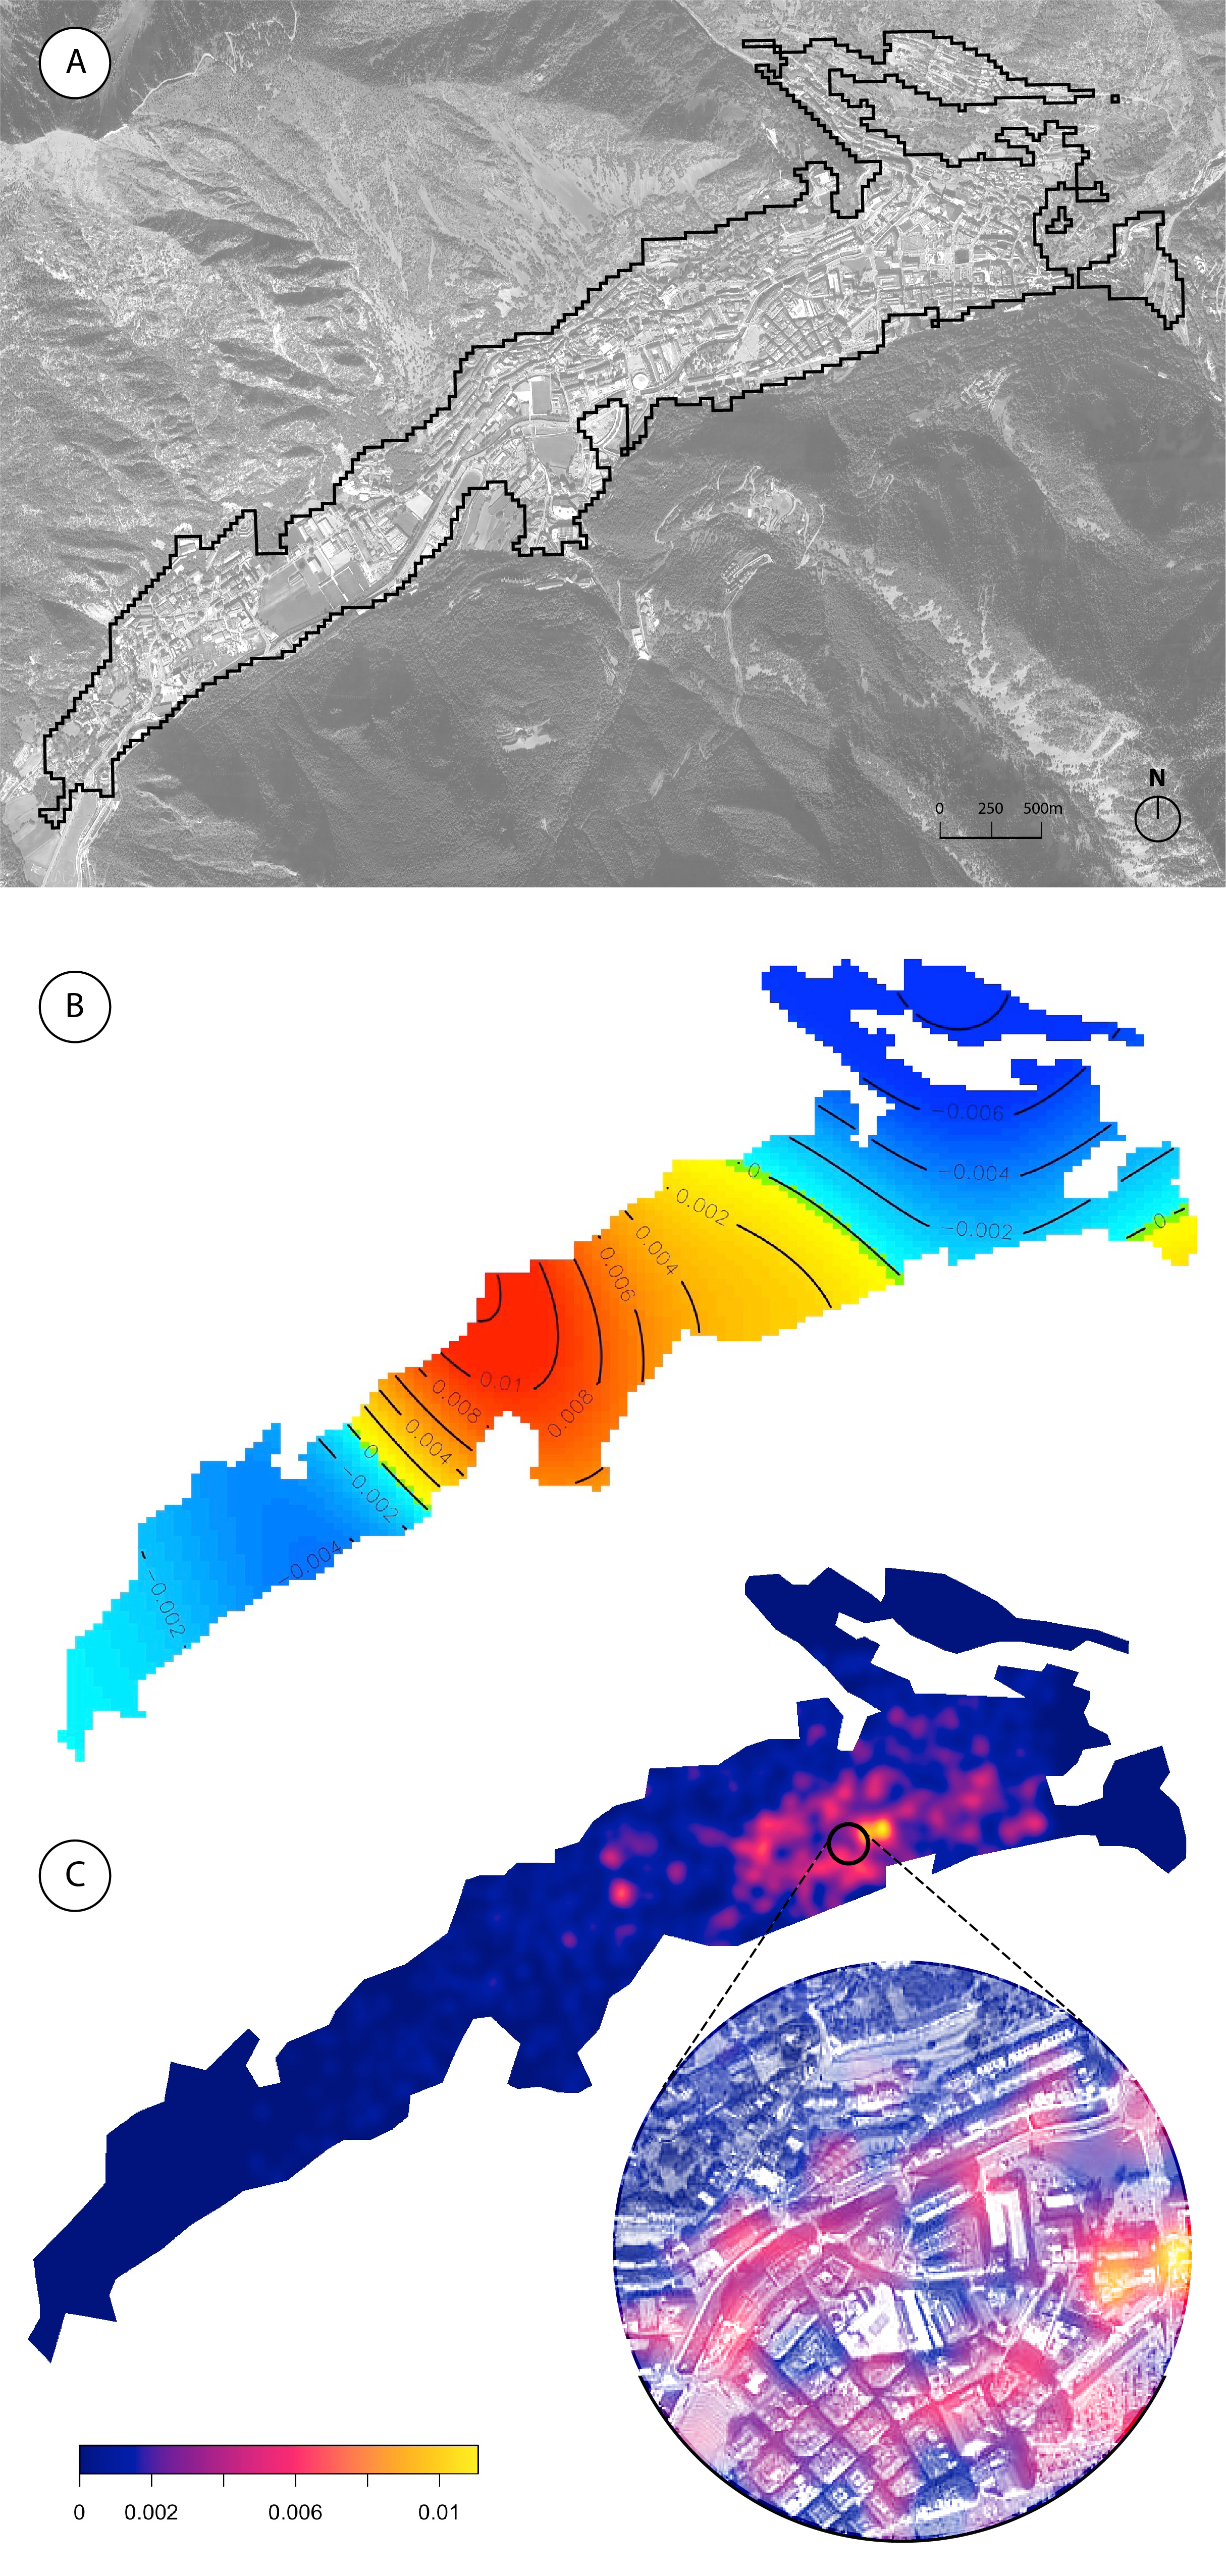
\includegraphics[width=0.5\textwidth]{chapters/insight/revurb/figures/revurb_ppm.jpg}
        \caption{Model area and densities. (a) Study region, (b) Contour plot of Pearson residuals from fitted model, (c) Smoothed density of points simulated from Inhomogeneous Poison Process model}
        \label{fig:ppm_res}
    \end{figure}

    The step-wise selection procedure outlined in Section \eqref{sec:ppm} resulted in a model which included 14 of the 16 urban features considered. The only variables excluded due to their failure to improve the AIC were Food and Education amenities. The coefficients of included variables and their significance levels are presented in Table \eqref{tab:results}.

    \begin{table*}[!h]
        \centering
        \caption{Results of Model Fitting}
        \label{tab:results}
        \begin{tabular}{ c|cccc }
            \hline
                       & Feature                & Estimate & Standard Error & Significance \\
            \noalign{\hrule height 0.5pt}
                       & (Intercept)            & -6.33    & 0.08           & ***          \\
            Amenities  & Entertainment          & 2552.53  & 302.75         & ***          \\
                       & Government             & 1068.22  & 235.25         & ***          \\
                       & Hotel                  & -1303.1  & 201.03         & ***          \\
                       & Religion               & 1191.52  & 424.82         & **           \\
                       & Service                & 827.62   & 39.79          & ***          \\
                       & Shopping               & 160.18   & 15.12          & ***          \\
                       & Car Parks              & 1.15     & 0.06           & ***          \\
                       & Bus Stop               & 2030.52  & 187.35         & ***          \\
            Distances  & d\_Motorized\_Streets  & -0.01    & 0.001          & ***          \\
                       & d\_Pedestrian\_Streets & -0.001   & 2.7E-4         & ***          \\
                       & d\_City\_Center        & -7.9E-4  & 4.5E-5         & ***          \\
            Urban Form & Water                  & 1.22     & 0.08           & ***          \\
                       & Green Space            & -14.34   & 202.56         &              \\
                       & Buildings              & 0.13     & 0.05           & **           \\
            \hline
        \end{tabular}
    \end{table*}

    The kernel smoothed density of a point pattern simulated from the model is provided in Figure \eqref{fig:ppm_res} (c). A 3-dimensional contour plot is also provided in
    Figure \eqref{fig:ppm2} to illustrate how the model could be used to graphically depict the expected density of social activity in an urban district.


    \begin{figure}[!h]
        \centering
        \includegraphics[width=0.6\textwidth]{chapters/insight/revurb/figures/revurb_ppm2.jpg}
        \caption{Perspective contour plot of point pattern simulated from Inhomogeneous Poison Process model}
        \label{fig:ppm2}
    \end{figure}


    \subsubsection{Validation and Predictabilty}
    {
        Validation of the IPP model can be done using both formal and informal methods. The likelihood ratio test is an appropriate formal method for Poisson processes \cite{baddeley2006modeling}. This can test the null hypothesis of a Homogeneous Poisson Process in favour of the alternative hypothesis of an Inhomogeneous Poisson Process with intensity that is a log-linear function of the final set of features. An extremely small p-value is found for the final model in this study, indicating that the null hypothesis should be rejected in favour of this model. The informal methods involve visual inspection of the model residuals.
        \newline
        Figure \eqref{fig:ppm_res} (b) shows a contour map of the residuals of the final model. This plot indicates that, despite the high statistical significance of the features included in the model, there are still some areas of the urban district where intensity is over-predicted and other areas where it is under-predicted. This suggests that there are some features missing from the model which could improve predictive power. Nonetheless, since many of the features which were included were strongly associated with cluster intensity, valuable insights about urban behaviors can still be gained from this model.
    }

    \begin{figure}[!h]
        \begin{center}
            \includegraphics[width=1\textwidth]{chapters/insight/revurb/figures/revurb_cell_results.jpg}
        \end{center}
        \caption{Model inference on a single grid-cell. The urban features are highlighted on the left, with their modelled coefficients on the right.}
        \label{fig:revurb_cell_results}
    \end{figure}

    \subsubsection{Results and Insights}

    {
        A number of key insights could be drawn form the fitted models. First, certain amenities were associated with clustering intensity with high statistical significance. In particular, bus stops, car parks, and amenities categorized as Entertainment, Government, Religion, Service and Shopping were positively associated with clustering. The only type of amenity which was negatively associated with clustering was Hotels. Clusters were much more likely to occur closer to the city centre and closer to roads, both motorized and pedestrianized. Of the urban form elements, both natural water elements and buildings were positively associated with clustering.
        \newline
        Perhaps most surprisingly, green spaces, which are commonly perceived as desired public spaces for diverse and long-lasting gatherings, were negatively associated with clustering; This association was not statistically significant but the variable was included in the model as it improved the AIC. This detraction pattern might be explained by the definition of clusters based on density: Although parks and other green spaces are typically popular places for people to stay, the concentrations of people can be expected to be sparser than, for example, the confines of a shopping street.
    }
}

\subsection{Discussion}
{
    This study has demonstrated a methodology for assessing the performance and degree of activity of urban spaces, given spatial and telecoms data. The methodology found statistically significant associations between several types of urban features and the tendency for activity clusters to form around them. The rest of this section will discuss the contribution, potential, and limitations of this work.

    \subsubsection{Limitations}
    {
        The region and time period covered by the RNC dataset were relatively small, making this study's result less generalizable. Moreover, differences in culture, geographical, and seasonal factors might produce different outcomes when applying this method to other regions. The data used were of high resolution compared to many urban studies \cite{Louail2014} but the resolution was still not high enough to infer, for example, usage of specific amenities by individuals. As well, the RNC dataset is subject to propitiatory and commercial restrictions; This prevents the data and the full details of the underlying algorithm to be publicly available. Lastly, while the model results showed that many of the considered urban features were statistically significant with respect to behavior, the residual plot revealed partial spatial correlation, indicating that certain features might be missing from the model.
    }

    \subsubsection{Contribution and Opportunities}

    {
        The main contribution of this work is in providing a methodology that can be used in an evidence-based city-planning process. Using this approach, planning actions could be evaluated based on their likelihood to encourage vibrant social activity or - if desired - the lack of it. Even if the model predictions may not be precise in terms of the exact locations and sizes of activity clusters, the effects of each type of feature can be accurately predicted in terms of direction and relative effect size. With more accurate data and more robust models, this approach could be used to hint to the effectiveness of future urban-design interventions, especially in `infill' projects.
        \newline
        Finally, this work demonstrated the potential of spatio-temporal data to be used for gaining high-resolution insights. In an evidence-based urban process, these insights can help assess the impacts of spatial interventions on human behavior, and thus the effectiveness of proposed interventions. As Chapter \eqref{ch:prediction} entails, these type of implicit models could be used to help forecast the likelihood of a certain action to occur or to change in accordance with urban transportation.
    }
}





\label{sec:revurb}
%%%%%%%%%%%%%%%%%%%%%%%%%%%%%%%%%%%%%%%%%%%%%%%%%


%%%%%%%%%%%%%%%%%%%%%%%%%%%%%%%%%%%%%%%%%%%%%%%%%%
\section{Discussion: From Data to Actionable Insights}

 {
  This Chapter discussed the potential of urban insights to inform decision-making in planning, mobility, energy, tourism, and other aspects. While some insights could be gained from viewing a narrow perspective of the city, more advanced urban insights are the product of superimposing many different observations and data layers, so that anomalies, edge-cases, and relevant questions would arise. If done right, insights are a powerful tool to initiate urban decision-making, and can begin to inform the development of urban policies, strategies, and counterfactual scenarios. Importantly, real-time and updated insights can reduce the risks associated with asynchronous planing processes, in which by the time development has started, the state of the city has already changed.
  \newline
  The next Chapter explore ways to utilize such insights in the process of transforming the built environment.
 }



%%%%%%%%%%%%%%%%%%%%%%%%%%%%%%%%%%%%
\chapter{Transformation}\label{ch:transformation}
{
    \section{Introduction}
     {
      As previously discussed (see Chapter \eqref{ch:insight}), the role of insights is to focus the urban discussion on specific challenges, and establish clear KPIs to evaluate future interventions. The next step is to introduce and evaluate change to the city, in the from of urban \textit{Transformation}: an iterative exploration of design interventions and policies, set to transfer the city from its current state to another. In CityScope, evaluating transformation is possible through a wide range of Urban Human Computer Interaction (UHCI) methodologies, systems, and interfaces. Unlike traditional city-planning practices, CityScope is built for synchronous design exploration, in which evaluation of many design proposals is conducted simultaneously, while being fed by real-time data and analysis. To achieve this capability, CityScope has two main streams of development: (i) \textbf{CityScope UHCI:} The creation of iterative user interfaces, both tangible and digital, and (ii) the design of \textbf{CityScope Modules:} real-time models, simulations, and metrics which provide feedback during design sessions\footnote{Chapter \eqref{chapter:introduction} and \eqref{subsec:emergence_uhci} explore the origins of UHCI, the state of the art tools and systems developed over the years, as well the challenges associated with this systems.}.

      %%%%%%%%%%%%%%%%%%%%%%%%%%%%%%%%%%%%%%%%%%%%%%%%%%

      \subsection{Urban Transformation: UHCI Systems and Case studies}
      {
          This chapter has two main parts: (i) The first details CityScope technologies that were developed for real-time, iterative, and interactive urban  decision-making processes. These include the development of a data standard across CityScope projects; the integration of different TUI, computer-vision systems, AR, VR, and other interfaces; and the development of a web-based, platform-agnostic interaction and feedback system for CityScope. (ii) The second part of this chapter explores the implementation of these technologies in key CityScope projects, focussing on their usability, impact, shortcomings, and potentials for future planning processes.
      }
     }

    %%%%%%%%%%%%%%%%%%%%%%%%%%%%%%%%%%%%%%%%%%%%%%%%%%
    \section{CityScope Architecture \label{sec:cityscope_architecture}}

 {
  \subsection{Introduction}
  {
      The previous Chapter discussed the role of insights as a way to converge on urban places and issue in need for a change (see Chapter \eqref{ch:insight}). In CityScope, the exploration of \textit{change} is achieved by iterating through many design interventions and policies, using a range of Urban Human Computer Interaction (UHCI) methodologies, systems, and interfaces. The design of CityScope as an end-to-end ecosystem of UHCI components was developed over several years. At first, components were developed in silos, which forced CityScope projects to be tightly integrated and single-use (see, for example, CityScope BRT \eqref{sec:brt}). The system described in this chapter is of CityScope as a modular architecture, which by-design allows for the integration of different components, and their reuse in new projects. In order to communicate between the different parts of the CityScope system, a common data schema was developed (`CityScope Schema'). This schema is used to store, exchange, and define the data types and semantics of the different components. Figure \eqref{fig:cs_arch} illustrates the modular design of CityScope and the transfer of data using the Schema.
      \newline
      The rest of this section details the architecture of the CityScope ecosystem, discusses the design of the communication and storage service (`cityIO'); urban analysis microservices (`CityScope Modules'); as well as TUI (`CityScoPy') and frontend (`CityScopeJS') clients.
  }


  \begin{figure}[!htb]
      \begin{center}
          \includegraphics[width=1\textwidth]{chapters/transformation/cs_arch/figures/arch/cs_arch0.png}
      \end{center}
      \caption{
          CityScope Architecture. This diagram presents the data flow and different components of the CityScope architecture: (purple) Different modules control the inputs and CityScope Grid interaction; (blue) Upon interaction, cityIO VPC handles the transaction with different analytics modules; (green) When the computation phase is completed, the grid and analysis modules results are sent to output devices, either online (CityScopeJS, API), or onsite (projectors, monitors)
      }
      \label{fig:cs_arch}
  \end{figure}

  \subsection{Schema and Types System}\label{subsec:types_system}
  {

      \begin{figure}[!htb]
          \begin{center}
              \includegraphics[width=0.8\textwidth]{chapters/transformation/cs_arch/figures/arch/cs_arch1.jpg}
          \end{center}
          \caption{Type System and CityScope Schema. This diagram presents three examples of basic and more complex types as CityScope grid tiles, and how they are encoded in the Schema using LBCS and NAICS codes. (Figure: Luis Alonso, MIT)}
          \label{fig:type_sys_schema}
      \end{figure}

      The CityScope Schema defines a set of \textit{`types'} that are used to describe land-uses, urban functions, and purpose of fixed-size, rectangular geographical-units. These units can then be combined and arranged to represent complex urban environments over a CityScope intervention area, or the  \textit{`grid'}. Types are assigned to all cells in the grid, providing unified segmentation, scale, and a level of abstraction, that can be easily manipulated by users in both physical TUI and virtual interfaces. Cells within the grid can either be immutable or amendable, depending on the project specifications; At minimum, each tile must include one LBCS land-use, but most modules would require also one economic activity. The land-use data is based on the LBCS land-use classification system \cite{montenegro2012land}, and the economic activity data is based on the NAICS codes \cite{NorthAme86:online}\footnote{
          \textit{Land Use Classification Notation} or LBCS classification system includes activity, function, building type, site development character, and ownership constraints in each of its dimensions (for LBCS scheme breakdown, see \eqref{appendix:schema-description}).
          \newline
          \textit{Economic Activity Classification Notation} or NAICS are a standard used by Federal statistical agencies in classifying business establishments for the purpose of collecting, analyzing, and publishing statistical data related to the U.S. business economy. Codes are generated using a numerical classification outlined in the NAICS manual \cite{NorthAme86:online} (for NAICS scheme breakdown, see \eqref{appendix:schema-description}).
      }.
      Types may differ from one project to another, depending on the desired intervention or research question. For example, a CityScope project might include types associated with different levels of energy consumption, in order to asses how certain spatial arrangements can change energy usage.
      \newline
      In order to transfer Schema data between the different components of CityScope, a server system called `cityIO' was designed. The next section details the evolution and design of this system.
  }


  \subsection{cityIO}\label{subsec:csarch-cityio}
  {

      \begin{figure}[!htb]
          \begin{center}
              \includegraphics[width=0.5\textwidth]{chapters/transformation/cs_arch/figures/arch/cs_arch2.png}
          \end{center}
          \caption{cityIO V1: Data flow in the early version of cityIO.}
          \label{fig:cityio_v1}
      \end{figure}


      \textit{cityIO} is a CityScope service responsible for the communication between the different components of the CityScope ecosystem. cityIO maintains the current and - in some cases - the past state of CityScope instances, as well as preform other server-side tasks, such as security and user-logging. In 2015, cityIO first version was created with the sole purpose of supporting communication between a tangible user interface (TUI) and a handheld AR device. That version was developed using User Datagram Protocol (UDP), a fast yet unreliable packets-based communication \cite{richard1994tcp}. When users interacted with the CityScope TUI (for example, by moving a LEGO tile), a packet would be sent to the server, and then broadcasted to the AR devices (see Section \eqref{sec:cityscope_ar}). With each interaction, the virtual environment in these devices would react with updated visualizations and analysis. UDP presented several challenges: (i) Its data reliability was limited, and lost data packets caused inconsistent user experience, (ii) UDP was not scalable to web-apps due to security concerns. In 2016, an HTTP server-client system has been proposed to allow more scalable and reliable communication between elements of the CityScope ecosystem.

      \subsubsection{cityIO Ver. 1 (`15-`18)}
      {
          The first version of cityIO was using an HTTP protocol and a REST API, which exposed a simple data packet called \textit{CityScope Grid}. The grid was digital translation of a 2D array of objects, which represented the state of the CityScope TUI; With each user interaction, the grid would update, and sent to the server. The server then stored the grid, so that other microservices or devices could access it. By design, cityIO did not limit the access and modification of the grid by other microservices or devices, so that its state could be updated from all ends of ecosystem (i.e., analysis services, other TUI, etc.). The Grid was a JSON object which included a list of lists; Each element in the list had two numerical variables: $[type, rotation]$. The `type' is a numeric index of a list of land-uses\footnote{These land uses could be as simple as as `offices', `housing', or `road', or more complicated types, such as `offices for large companies with retail at the bottom two floors'}, and the `rotation' is the rotation of the physical tile (i.e., 0 - facing up, 1 - 90° rotation, etc.). As such, a client reading the grid, would assume that the tile $[t,r]$ at position $[i,j]$ is of type $type_t$ and rotated $rotation_r$. A typical data sample of the grid object is shown in the Appendix \eqref{appendix:cityio_output_format}. This cityIO version was built with in NodeJS, python, and later in GO.
          \newline
          \textbf{Usage:} The HTTP bidirectional communication enabled users to not only obtain the state of the CityScope TUI, but also interact and share their opinion during real-time CityScope design sessions. For example, users could select geo-located spots in the virtual grid (such as buildings, parks or roads) and add textual comment to the designs proposed by other users, done by simply extending the JSON object of that grid-cell (for example, see the AR application in Andorra at Section \eqref{sec:andorra-data-observatory}). This type of communication offered designers, decision-makers, and communities a way to participate in a shared physical-virtual design session.
          \newline
          \textbf{Limitations:} First, the lean data structure of the grid was not easily interpretable by other microservices or end-user devices. Each microservice would have to parse the grid object, based on predefined Knowledge of the way the grid was structured. This created inconsistency when some microservices were parsing the grid differently from others. Second, the TUI responsible to share the grids' state, was often triggered by external events, such as light bursts, or a slight movement of the TUI table. This created a torrent of data packets flooding the server, which was not scalable, and created a bottleneck in slow-moving microservices. These issues were addressed in the next version of cityIO.
      }



      \begin{figure}[!htb]
          \begin{center}
              \includegraphics[width=.65\textwidth]{chapters/transformation/cs_arch/figures/arch/cs_arch3.png}
          \end{center}
          \caption{Converting a site to the CityScope Schema: (a,b) designating and aligning an urban intervention site (c) `pixelation' of the site's land-use using the Schema (d) building the TUI for the CityScope context}
          \label{fig:voxel_to_schema}
      \end{figure}


      \subsubsection{cityIO Ver. 2 (`18-current)}
      {
          Amidst these challenges, the second version of cityIO was designed more as a real-time database than a massaging service. The main difference was the implementation of a new CityScope Schema, that was assuming no prior knowledge of the grid, the contextual area, or other baseline information. Instead, the schema was designed as a single JSON object, which hold key-value pairs for the entire data needed for a microserviced CityScope instance. The bare minimum key-value pair is of one \verb|GEOJSON| object called \verb|GEOGRID|, which included all necessary information to render the grid, including geo-location of each grid-cell, their types, and other properties (see examples ver.2 in Appendix \eqref{appendix:cityio_output_format}). Using this object, CityScope users, clients, and microservices could understand the structure of the grid, and parse it in a user-friendly way.
          \newline
          Unlike the first version of cityIO schema, \verb|GEOGRID| is an immutable object, which should not be changed by other microservices. Instead, a mutable object called \verb|GEOGRIDDATA| was introduced, in which only the core properties of each grid-cell are stored. This object is smaller than \verb|GEOGRID|, and is constantly updated by the TUI or other microservices, as needed. The logic behind this design is to maintain a single source of truth for the grid with \verb|GEOGRID|, thus always preserving the initial `tabula-rasa' state of the site in question.
          \newline
          Additional key-value pairs in the root of the CityScope Schema are defined as `CityScope Modules' (see Section \eqref{subsec:cs-modules}), which are the aggregated analysis results of different computational modules or microservices. The next section describes how CityScope modules analyze and evaluate the grid data, and share their results with cityIO.
      }
  }

  \subsection{Microservices and Modules}\label{subsec:cs-modules}
  {
      As discussed in Section \eqref{sec:cityscope_architecture}, CityScope architecture is based on \textit{microservices}, which are a set of computer services that are designed to run independently of each other. The microservices are designed on different platforms and operating systems, so that each service can operate on its designated environment \cite{balalaie2016microservices}. This architecture stems from the idea that each microservice can be designed independently, as long as a shared terminology exist.

      \subsection{Microservices}
      {
          In the context of city-planning and spatial analysis, the CityScope ecosystem requires a wide spectrum of microservices; From straightforward calculations of square footage, to complex noise, energy, or traffic simulations. If in early stages, CityScope was composed of a single service for a single instance (such as the zoning simulation in CityScope Playground, see Section \eqref{sec:cityscope_playground}), the microservices design would allow for each CityScope to preform multiple tasks and analyze various aspects in concurrency.
          \newline
          Another motivation for the development of a microservices architecture, is the need to support the extension of CityScope interfaces beyond the TUI. Decoupling UI, feedback, and analysis microservices allows to add new interfaces, modules, and visualization aids without having to update the existing hardware or software. For example, projects like CityScope Corktown can be fully accessed on a web-browser, where CityScope Ho Chi Minh City would utilize a physical interface, all the while running the same underlying microservice architecture.
          \newline
          Lastly, the microservices architecture is designed to be easily extensible. Since a major aspect of CityScope is open-source and collaborative development, contributions to either frontend, backend, or individual microservices is made possible using detached components. In that manner, the teams working on CityScope Grasbrook (see Section \eqref{sec:grasbrook}) were able to extend the CityScope ecosystem to include new microservices, add functionality to existing ones, as well as redesign the frontend and TUI components as needed.
      }


      \begin{figure}[!htb]
          \begin{center}
              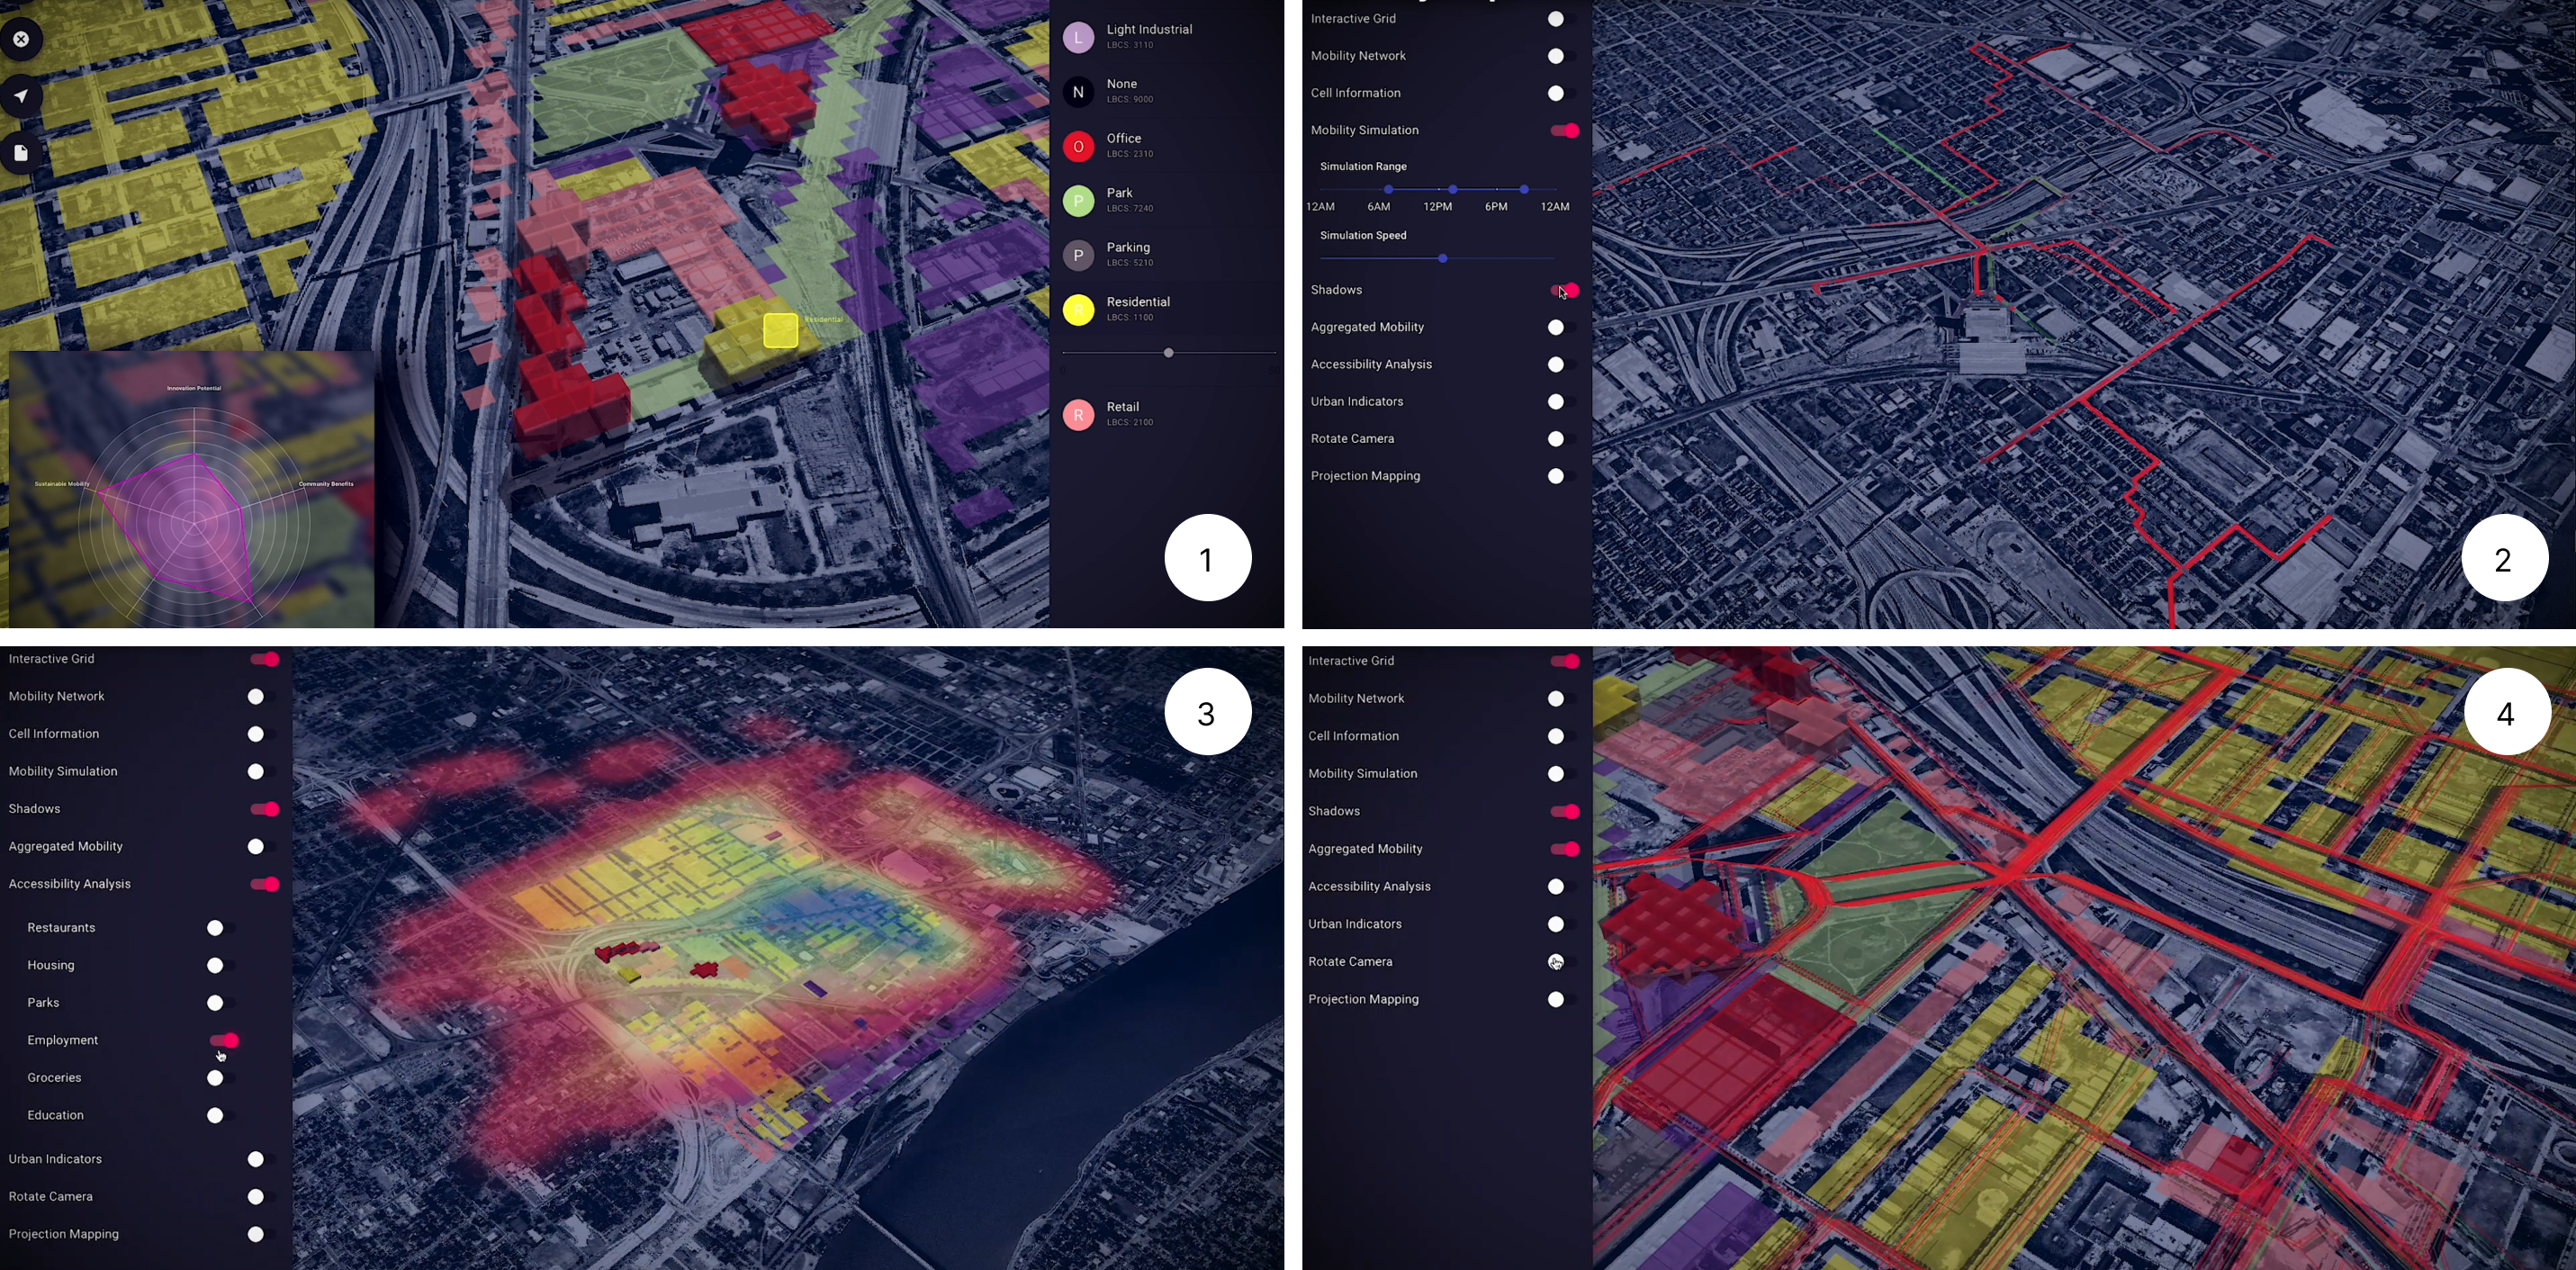
\includegraphics[width=1\textwidth]{chapters/transformation/cs_arch/figures/csjs/csjs_0.png}
          \end{center}
          \caption{CityScopeJS interface. Similar to the TUI versions of CityScope, users interaction is design to be simple and intuitive. Interactions are sent to the cityIO analysis modules, and their responses are then displayed spatially as heat-maps, trips, or graphically as charts and data visualizations. (1) CSjs grid design using a `paintbrush' gesture; (2) animated results of mobility analysis module; (3) results of accessability heatmap to employment and other urban attributes; (4) accumulated traffic results and mobility mode for each road segment.}
          \label{fig:csjs}
      \end{figure}



      \subsection{Modules}
      {
          CityScope Modules is a collection of backend microservices which preform the analysis for a CityScope project. Every time a user interacts with the CityScope interface (via virtual or physical UI), their \verb|GEOGRIDDATA| state is updated on the cityIO server; Modules are constantly listening to these changes, and are triggered to preform analysis with each change.
          When a CityScope module completes an analysis, its results are sent back to cityIO, so that the frontend, and other modules, would have access to it. The analysis results are called `indicators', which can be any of numeric, heatmap, simulation, or textual representation. Numeric indicators are usually displayed as a chart (bar, radar, etc. See Section \eqref{sec:cityscope_volpe}). Heatmap indicators are geo-located (points, lines, or polygons) which are displayed as layers directly on the CityScope table. Simulations are also displayed on the table but are the result of a temporal analysis (such as ABM, mobility simulation, etc) and are therefore displayed as a dynamic layer.
          \newline
          Some modules' results are not directly visualized on the CityScope interface. Instead, these modules would only compute so that other modules could use their results, as part of their analysis. For example, a CityScope table dedicated to the analysis of noise in a new development site, would use mobility simulation to indicate the types and volume of vehicles traversing through the area. The results of this mobility module would not be used for visualization, but instead would become available for the noise module itself. This structure allows greater complexity and dependency of analysis modules. To ensure all modules are synced with the current state of the \verb|GEOGRIDDATA|, cityIO produces a unique hash for each grid state (see Appendix \eqref{appendix:cityio_output_format}). The next section describes how modules' results and user interaction are combined in the CityScopeJS frontend.
      }
  }



  \begin{figure}[!htb]
      \begin{center}
          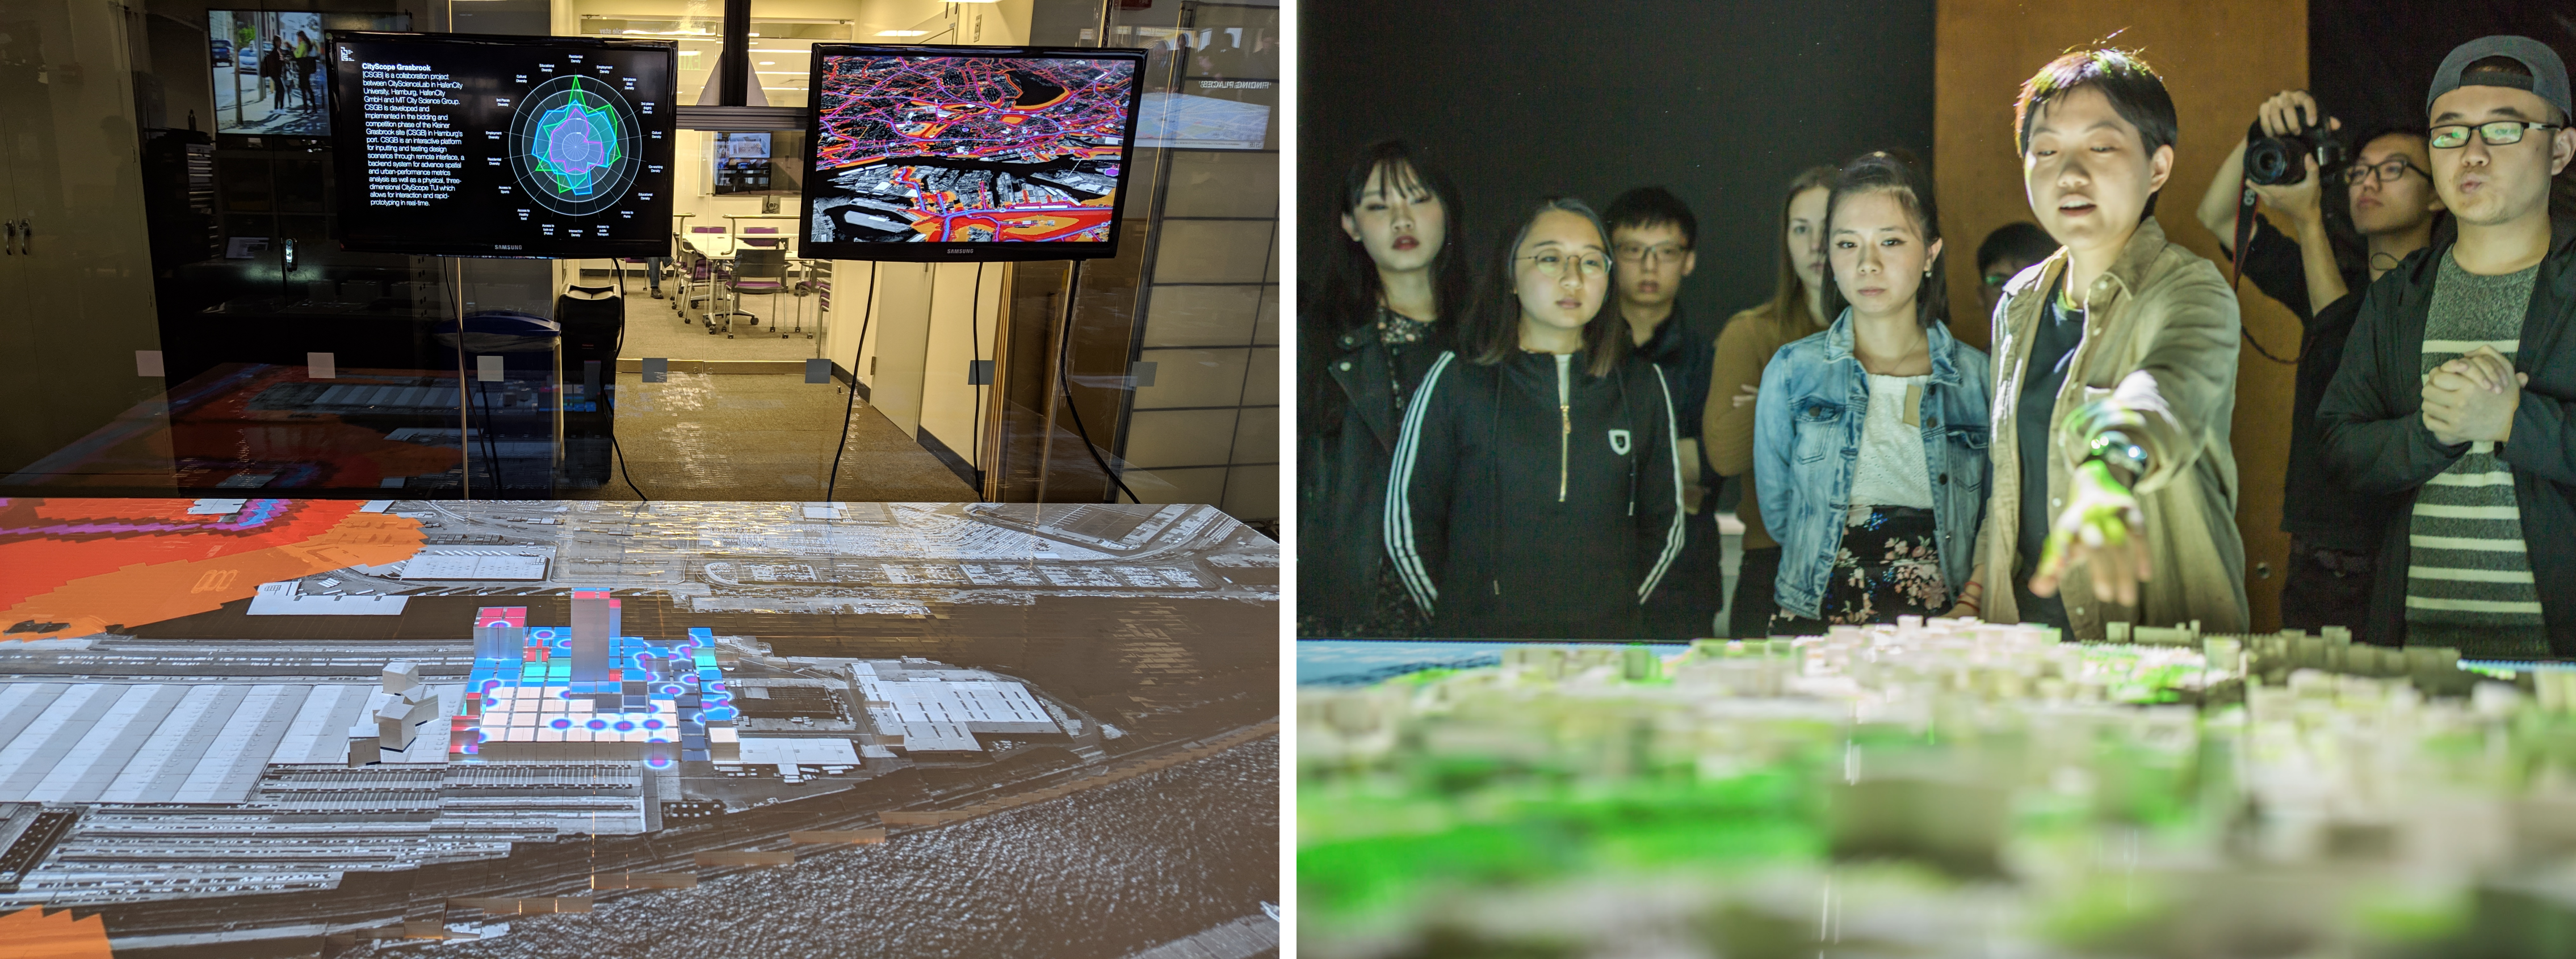
\includegraphics[width=1\textwidth]{chapters/transformation/cs_arch/figures/csjs/csjs_1.png}
      \end{center}
      \caption{CityScopeJS usage in tangible interfaces. (left) CSjs for the Grasbrook project in Hamburg \eqref{sec:grasbrook}; (right) an early version of CSjs for a student workshop in Aalto University, Espoo, Finland.}
      \label{fig:csjs_tui}
  \end{figure}

  \subsection{CityScopeJS (`CSjs')}
  {
      CityScopeJS\footnote{stands for CityScope Javascript or `CSjs' in short.} is the unified online frontend for the CityScope ecosystem. CSjs is designed to combine the most common use-cases for any CityScope instance: initiation, interaction, visualization, and feedback. CSjs allow users to examine different urban-design alternatives and understand their impact, through a range of KPIs, metrics, visualizations, and charts. It can be used as a standalone online tool, or in combination with TUI in an physical setting. Using its interface, users can edit a grid and change land-uses, buildings, open spaces or transport routes, as well as amend their properties and attributes. As soon as the user concludes their design session, their grid state is sent to cityIO for calculations by the modules. When these are computed, CSjs pulls the new analysis results from cityIO, and displays them on the interface. CSjs is built with ReactJS and DeckGL \cite{ReactAJ49:online,deckgl17:online}. The rest of this section describes the features of CSjs.

      \begin{figure}[!htb]
          \begin{center}
              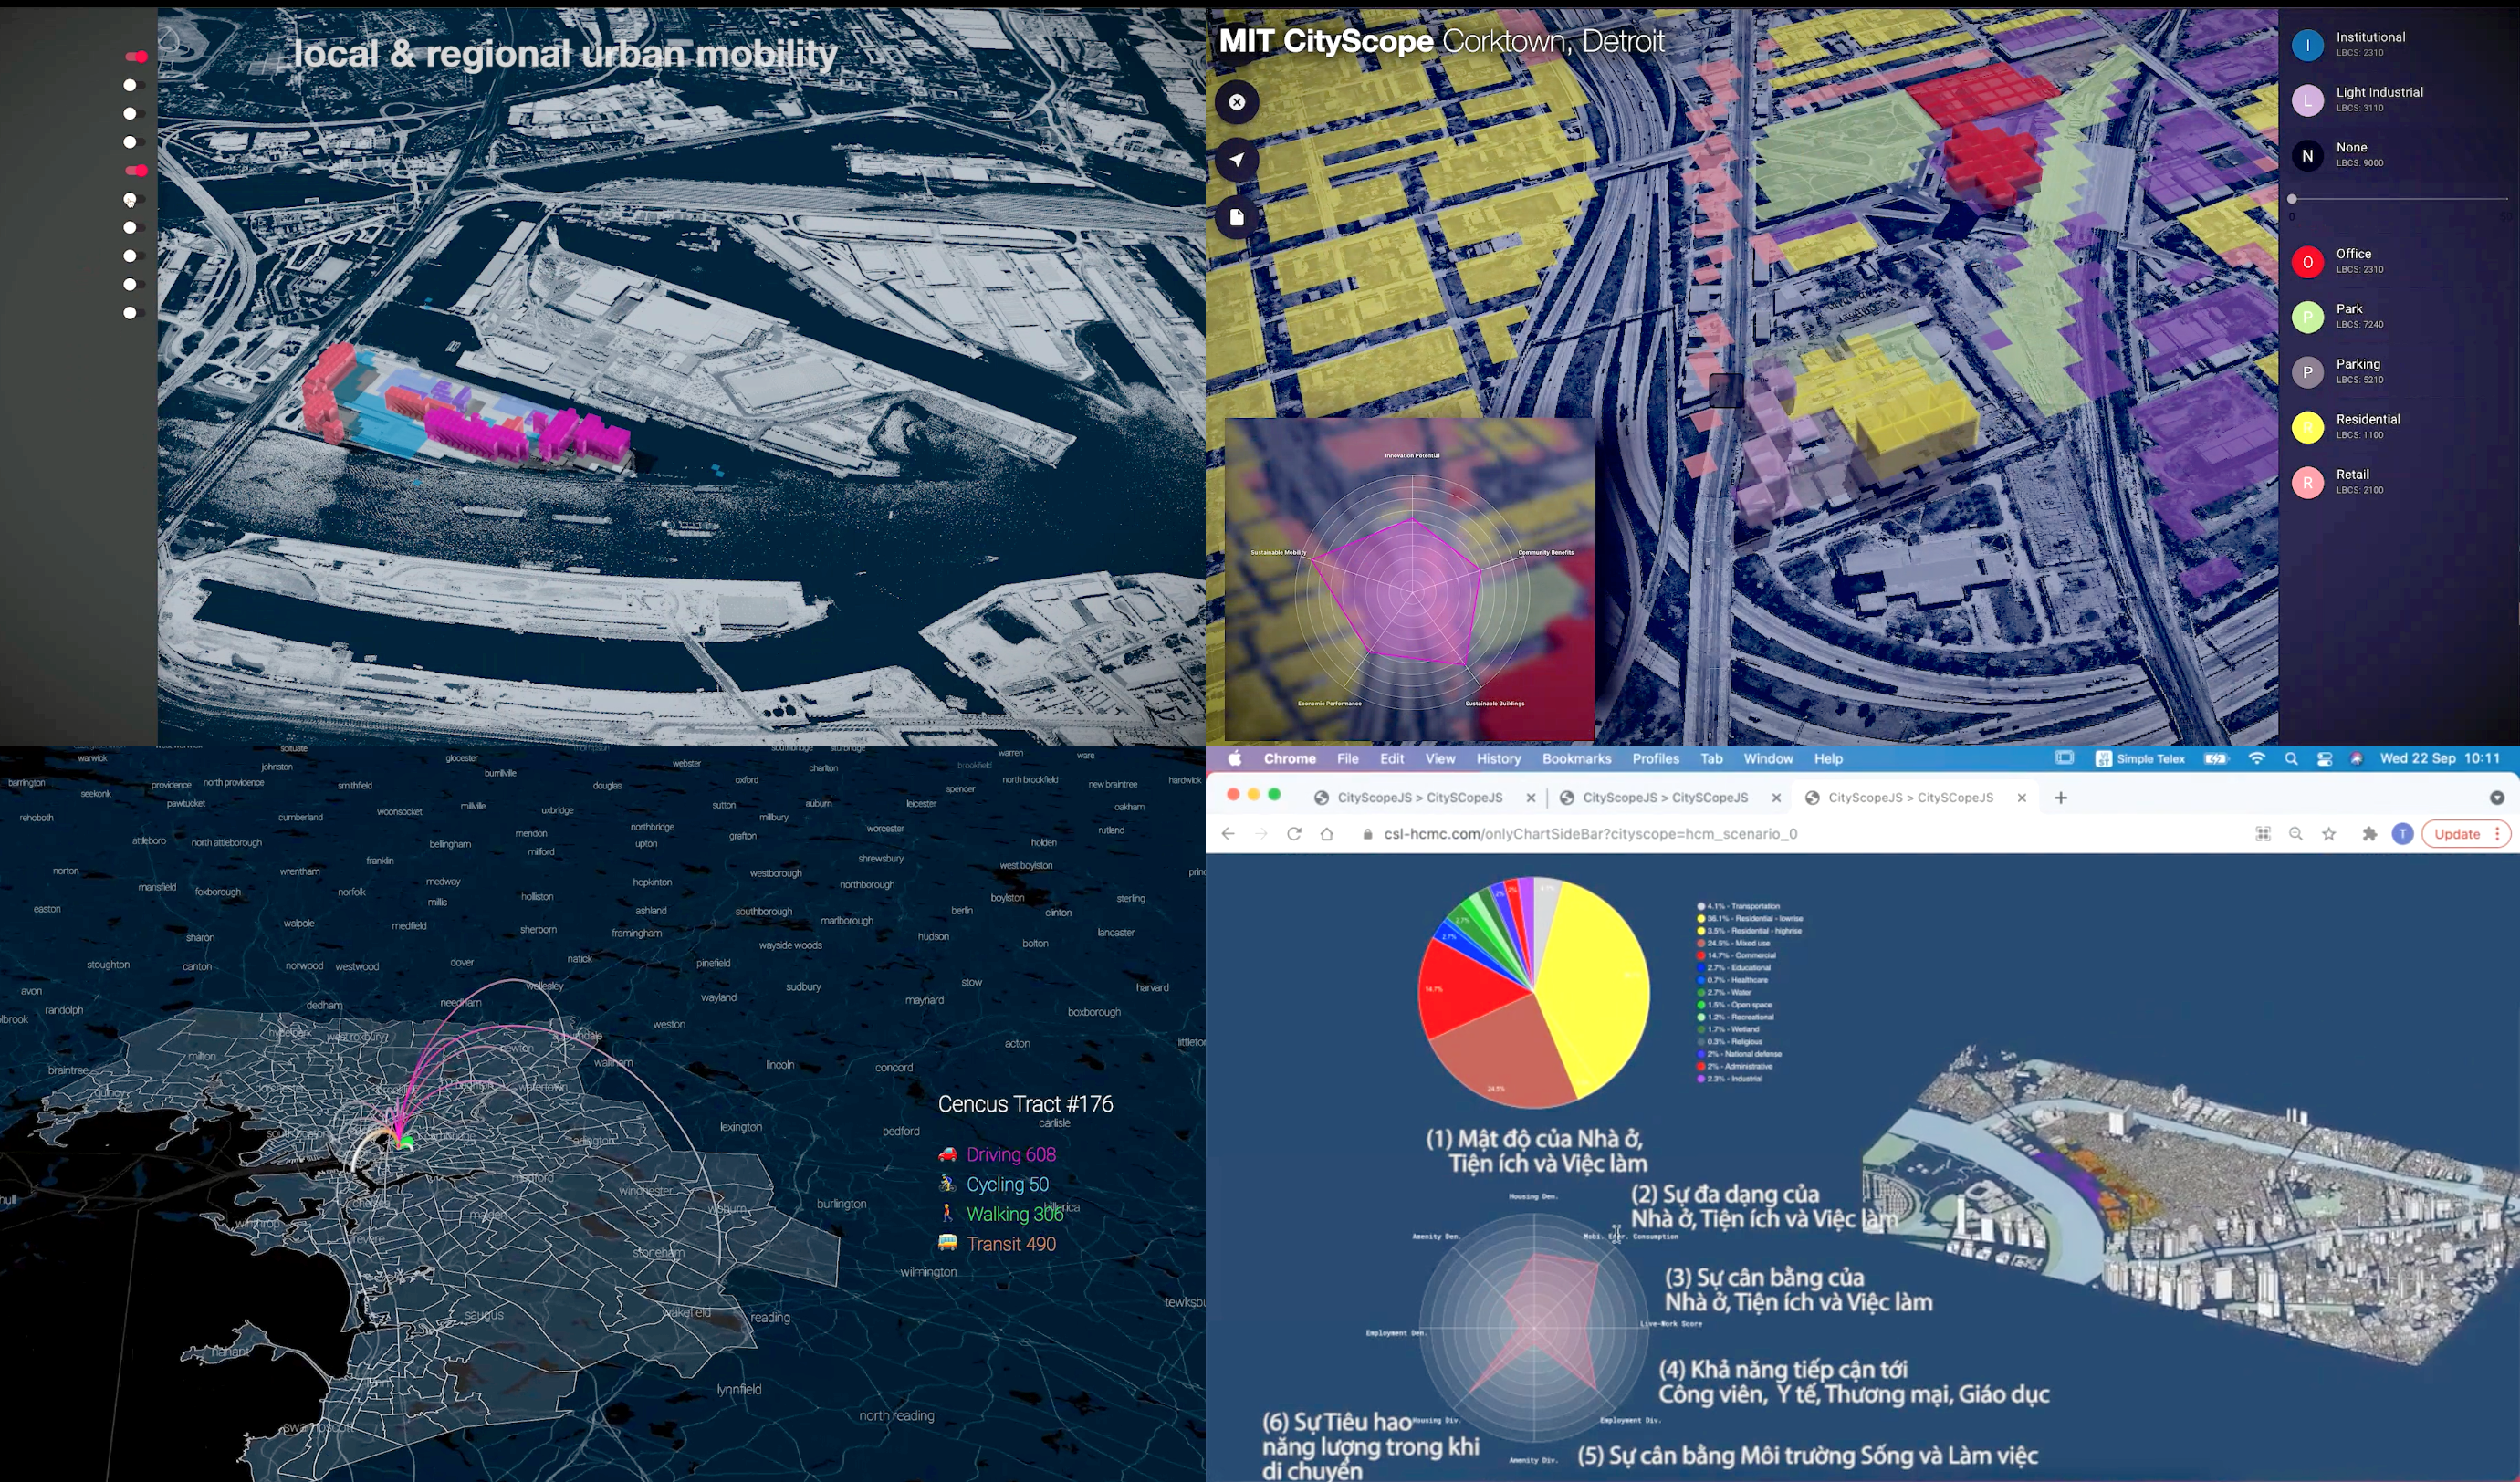
\includegraphics[width=1\textwidth]{chapters/transformation/cs_arch/figures/csjs/csjs_2.png}
          \end{center}
          \caption{CityScopeJS case-studies. (top-left) CSjs for the CityScope Grasbrook project in Hamburg, 2019 \eqref{sec:grasbrook}; (top-right) CSjs for the Corktown project in Detroit, MI, 2020; (bottom-left) CSjs for the CityScope MoCho, 2018 \eqref{sec:cityscope-mocho}; (bottom-right) CSjs for the Ho Chi Minh City project in Vietnam, 2021.}
          \label{fig:csjs_versions}
      \end{figure}


      \subsubsection{CSjs Features}
      {
          CSjs exposes three main features: \textit{Grid Editor}, \textit{Playground}, and \textit{Projection}. The CSjs Grid Editor is a helper tool to initialize and bootstrap new CityScope projects. It allows the creation of (i) a CityScope endpoint on cityIO (with a dedicated URI); (ii) a virtual, geo-located, 3D, and editable CityScope grid; and (iii) a list of `types' to be used in the design of this CityScope instance. The definition of types and their attributes strictly follows the aforementioned CityScope Schema (see Subsection \eqref{subsec:types_system}).
          \newline
          The \textit{CSjs Playground} is where users interact with the predefined CityScope grid. The interface is built to allow for simple, intuitive, and real-time intervention with the grid setup and land-uses, mimicking the ease of use of a traditional LEGO TUI. Unlike other CAD and planning tools, CSjs interface features minimal functions, toolbars, or menus, and is designed to be used with simple hand gestures on various devices, from an 9 ft TUI table, to a handheld cellphone.
          \newline
          Lastly, the \textit{CSjs Projection} is a tool to visualize the results of the CityScope modules on a TUI interface, such as a tangible grid. This is a passive presentation tool, that listens and renders updates directly from cityIO, without user interaction. This tool uses non-affine projection mapping (homography algorithm) that is designed to render the CityScope Grid and modules results on a physical interface using projectors.
      }

      \subsubsection{CSjs Case Studies}
      {
          CSjs development became a standalone effort in 2019, but was preceded by several projects and experiments since 2017\footnote{Such as CityScope MoCho, see Section \eqref{sec:mocho_api}}. The goal of these was to test the feasibility of web-based CityScope instances. With the increased power of web-based rendering, GPU acceleration, and faster computation, it became clear that many aspects of the CityScope ecosystem could be migrated to the web.
          \newline
          The development of CSjs was boosted by the CityScope Grasbrook project, which presented a real-world use-case for an online, distributed, and collaborative urban-design tool (see Section \eqref{sec:grasbrook}). since 2017, the majority of CityScope projects were built on top of CSjs, such as the Grasbrook, Corktown, EPA, Ho Chi Minh City, Guadalajara, and others. In some cases, developers built their own custom modules, frontend components, or connected CSjs to other TUI. For example, the RoboScope\footnote{see \url{https://www.media.mit.edu/projects/roboscope/overview/}}, an actuated TUI inspired by the MIT Tangible Media inFORM table \cite{follmer2013inform}, uses CSjs to link its TUI to the rest of the CityScope ecosystem. The next subsection describes how other TUI and interfaces are integrated in CityScope.
      }
  }

  \begin{figure}[!htb]
      \begin{center}
          \includegraphics[width=1\textwidth]{chapters/transformation/cs_arch/figures/cspy/cspy_0.jpeg}
      \end{center}
      \caption{CityScope TUI. Physical 3D urban models, scanning module, feedback monitors and projection scheme. Variations of this setup were used in many CityScope projects.}
      \label{fig:cspy_tui}
  \end{figure}

  \subsection{CityScoPy}\label{subsec:csarch-cityscopy}
  {
      CityScoPy is a TUI library for CityScope written in Python. It is designed to recognize interactions with physical objects equally distributed over a 2D grid (such as LEGO tiles), and send the scanning results as a JSON object to cityIO (see Appendix \eqref{appendix:cityio_output_format}, \eqref{appendix:cityscopymethods}). CityScoPy exposes several functionalities, such as keystoning, scanning, and sending data to different endpoints, as part of the microservices architecture of CityScope. CityScoPy is built in Python and OpenCV for image processing \cite{opencv_library}.


      \begin{figure}[!htb]
          \begin{center}
              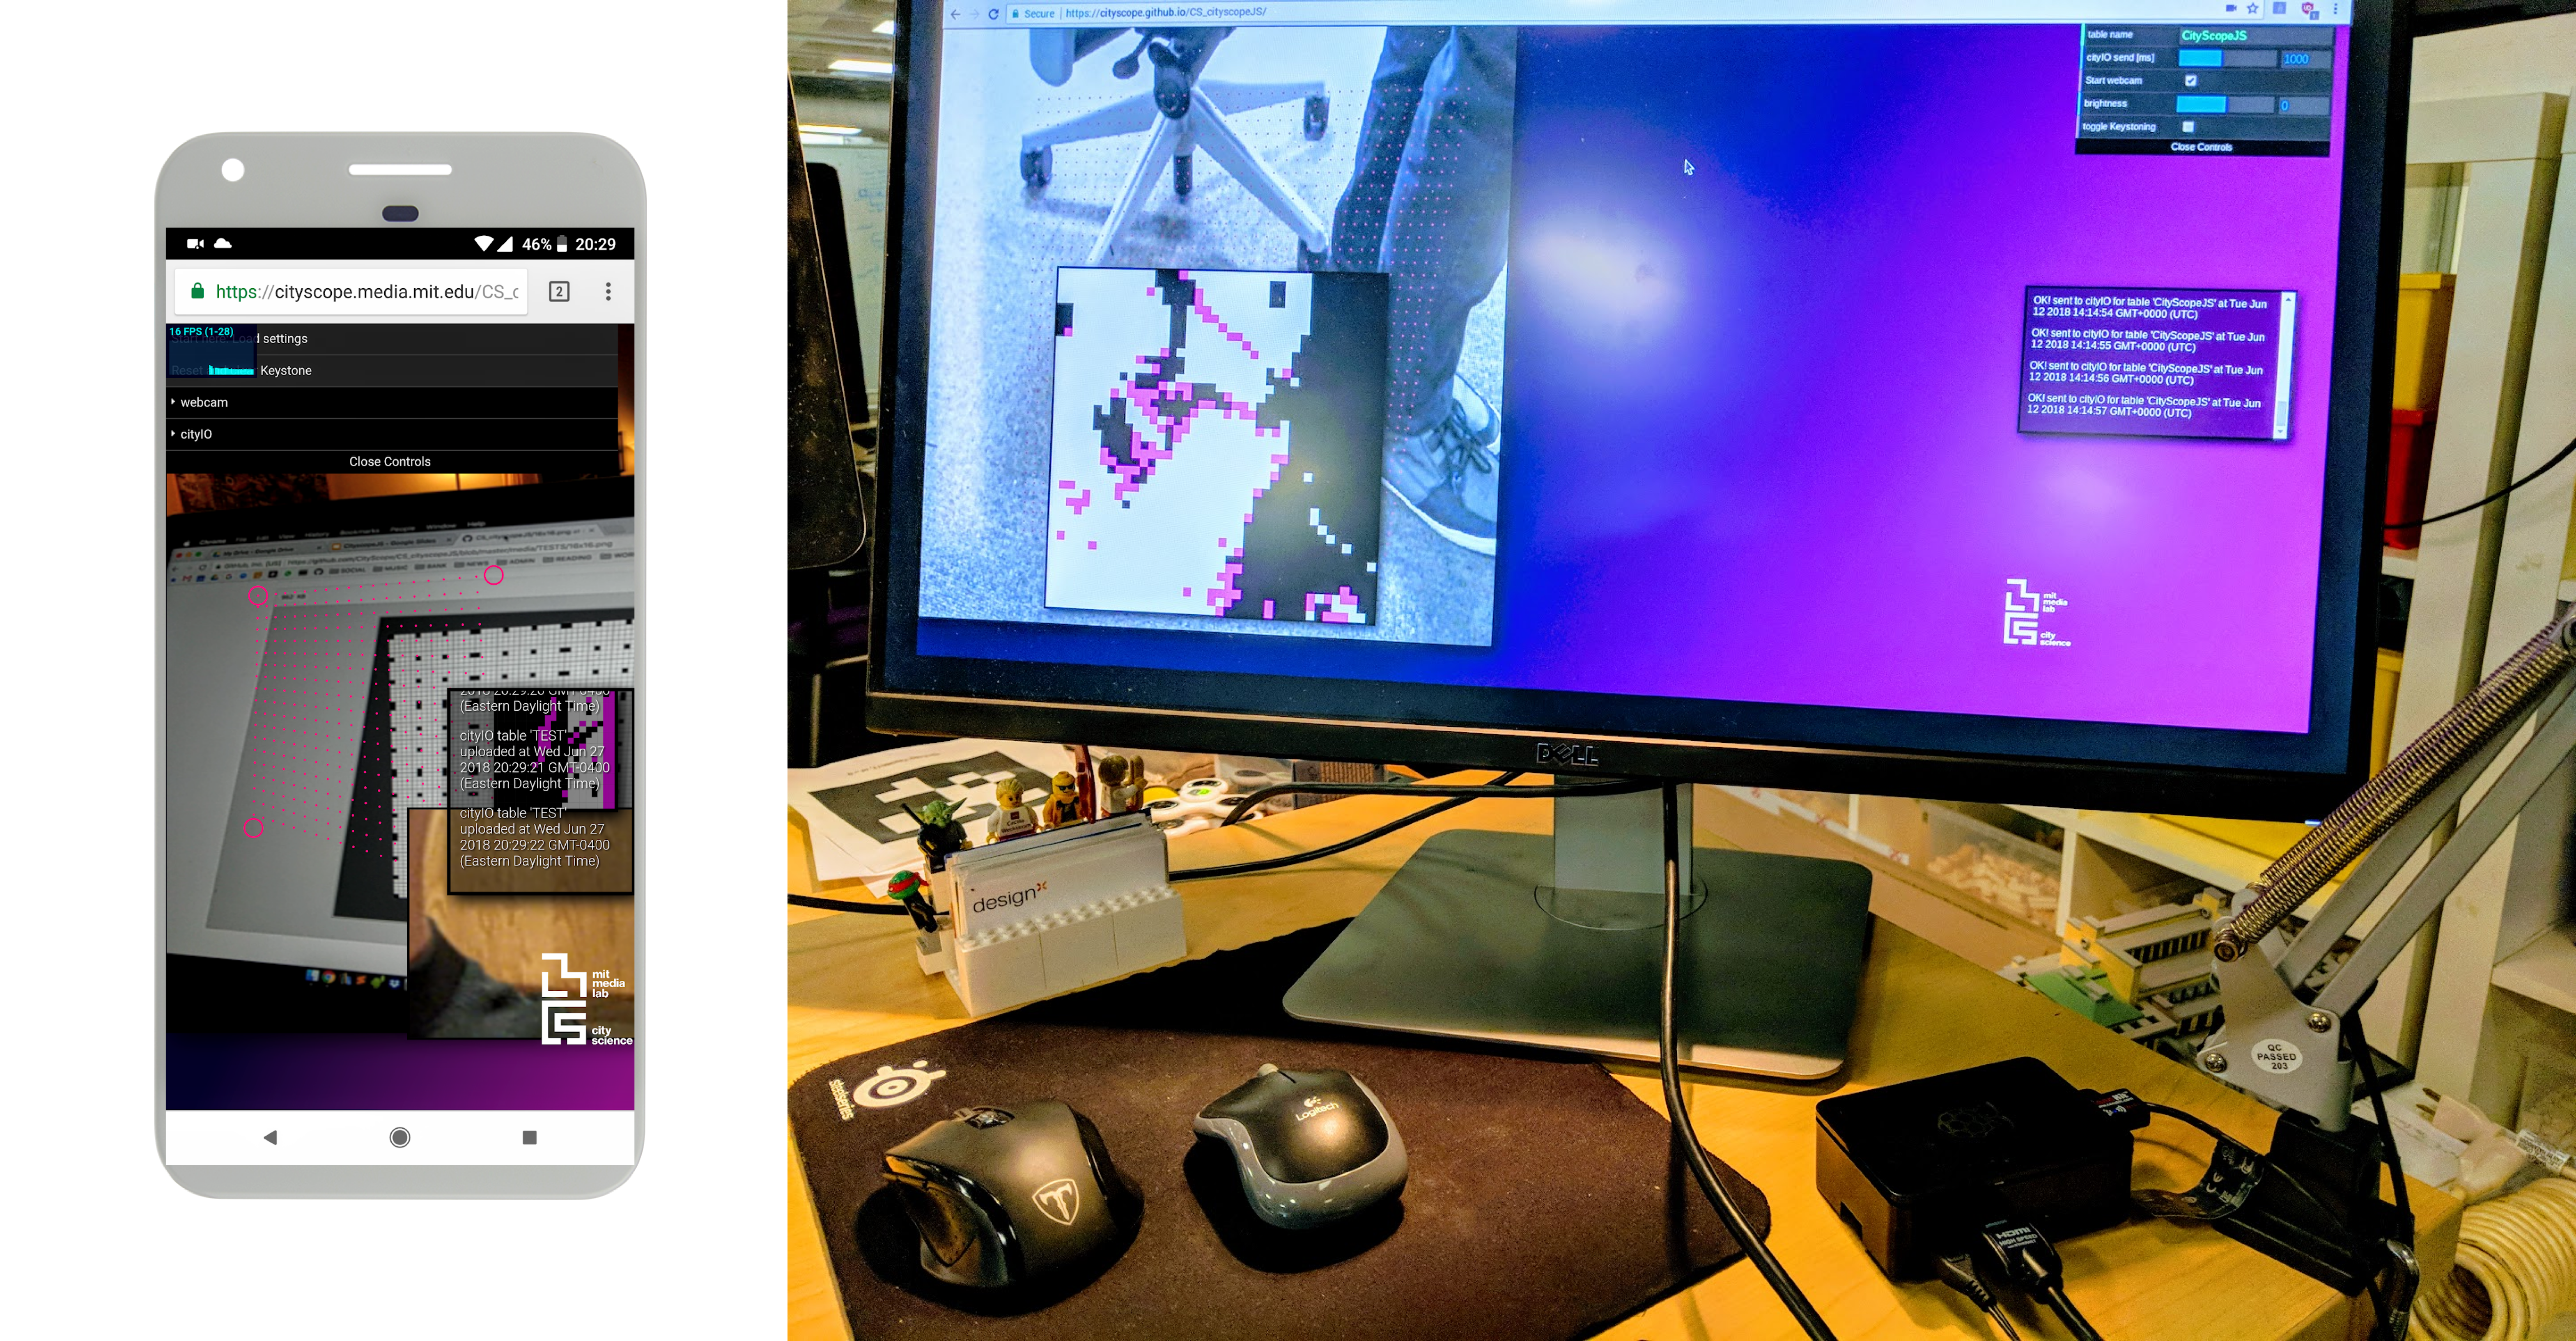
\includegraphics[width=1\textwidth]{chapters/transformation/cs_arch/figures/cspy/cspy_2.png}
          \end{center}
          \caption{CityScoPy scanner in action. This version of CityScoPy was created in vanilla Javascript to run on low-tier devices, such as cellphones or Raspberry-Pi with a basic web browser. Later versions were written in Python for faster scanning of larger grids.}
          \label{fig:cspy_scan_in_action}
      \end{figure}

      \subsubsection{Background}
      {
          CityScoPy is part of a long line of scanning tools developed over the years to support TUI for spatial analysis. Sensing the location of physical objects on a tabletop was prototyped in the exhibition ``Unbuilt Ruins''\footnote{By Kent Larson, displayed in Penn Architecture Archives (1999) and at `The Un-Private House' in the MOMA, NYC (1999)}, which featured digital-physical objects poised on top of a Louis Kahn's building blueprint \cite{sparacino1999technologies}. As users repositioned the objects, an array of projectors reviled rendered images associated with that object's location. Similar ideas were developed in the SandScape table \cite{ishii2004bringing}, where a digital relief of physical objects was captured in real-time using a top-down scanner. Since 2013, several scanning methods were developed by the CityScope team to capture physical objects and use them to simulate intervention and perform urban analysis \cite{Hadhrawi2016, zhang2017citymatrix, aldawood2014interaction}. These tools all shared the idea of scanning an array of predefined set of objects from beneath a translucent tabletop. The objects types were differentiated using colorful LEGO pieces, and the scanner was designed to recognize the objects' type and locations as users interact with them.
      }
      \subsubsection{Motivation and Design}
      {
          \begin{figure}[!htb]
              \begin{center}
                  \includegraphics[width=1\textwidth]{chapters/transformation/cs_arch/figures/cspy/cspy_3.png}
              \end{center}
              \caption{Example of a CityScoPy scanning result. The grid is scanned for binary values, and a 2D matrix is created to represent the grid cell. For each cell, a key-value pair search is conducted to find the corresponding type in the CityScope Schema.}
              \label{fig:cspy_results}
          \end{figure}

          CityScoPy was developed in order to improve several shortcomings in previous CityScope scanners: (i) \textit{Speed:} CityScoPy was designed to handle larger and more complex CityScope grids than before (see \eqref{subsec:vople_cityscope})\footnote{When tested on a 2015 Macbook Pro, CityScoPy scanned a grid of 100x100 4x4 LEGO tiles (total of 160000 scanned items) at 40fps.}. (ii) \textit{Versatility:} CityScoPy introduced a simple binary code, in which each of the LEGO studs of a 4x4 tile would be considered as either white or black\footnote{For example, a pattern with 4 white dots in the top-left corner and black in the rest would be [1,1,0,0,1,1,0,0,0,0,0,0,0,0,0,0].}. Using hues at the edges of the color gamut simplified the scanning algorithm, while still yielding $2^{16} = 65536$ unique permutations. This offered greater flexibility than the previous versions, while maintaining a simple way to differentiate types. (iii) \textit{Stability:} Previous CityScope scanners used a combination of colorful objects to identify types. These were proven unstable, since the scanner would tend to observe the same color at different parts of the tabletop as different RGB values. Since CityScoPy uses a binary code to define each type, the possibility of errors are reduced to the edge cases in the center of a gray-scale gamut. Additionally, the scanning algorithm captures and averages an array of 10x10 pixels for each scanning point, in order to reduce the potential of a faulty reading due to hazing or light bursts.
      }
      \subsubsection{Use-cases}
      {
          CityScoPy was adapted for several projects in HafenCity University, including the SmartSquare \cite{bley2020smartsquare} and CityScope Grasbrook \cite{baeza2021cityscope}. It was also used in several City Science network labs, such as Shanghai, Aalto, Guadalajara, and Jerusalem. At MIT, it was used for CityScope MoCho \cite{doorley2019s}, DeepScope \cite{noyman2020deepscope}, among others. In 2018, CityScoPy was used as part of an interactive installation for `The Road Ahead: Reimagining Mobility' exhibition in the Cooper-Hewitt Museum of Art, NYC \cite{CityScop40:online}. This CityScope artistically featured two extreme versions of a future with driverless cars: In one scenario, streets are dominated by vehicles which lead to congestion and anxiety; The other is a more vibrant city, where the benefits of walkability, mixed-use, density, and equity increase. In this context, CityScoPy allowed visitors to playfully interact with a fictional NYC-like urban grid, and impact the density and organization of the urban-scape in these two scenarios.
      }
  }

  \subsection{CityScopeAR}\label{sec:cityscope_ar}
  {
      \subsubsection{Introduction}
      {
          As discussed in Section \eqref{sec:cityscope_architecture}, the CityScope system design allows new ways to interact, visualize, and extend CityScope beyond the limitation of physical objects. CityScopeAR is a mixed-reality interface for CityScope, designed for remote yet collaborative urban-design processes. CityScopeAR builds on prior art using mixed-reality devices for CAD and urban-planning purposes (see Chapter \eqref{chapter:introduction}). The goal of CityScopeAR is to use hand-held devices such as smartphones, tablets, AR glasses, or VR headsets, and create a virtual environment that extends the tangible interface of CityScope, allowing users to interact with both the physical world and its virtual representation.
      }

      \subsubsection{System Design}

      {
          As discussed above in Section \eqref{subsec:csarch-cityscopy}, CityScope TUI tend to include a 3D urban model, projectors, and sensors to detect user interactions. Previous usability studies found several shortcomings in these setups \cite{Noyman2015power, Alrashed2015}: First, CityScope tables use flat-top tangible pieces projected with symbols and colors. In active participatory sessions, tables tend to get obstructed throughout most of the session, thus not communicating information as needed. Second, is the challenge of mixing different layers of information onto a single TUI; In user studies (see Section \eqref{sec:brt}), users requested different data layers to be displayed simultaneously. For example, experts might want to view traffic simulation, while member of the community wish to view the noise analysis layer. Lastly, CityScope TUI had no mechanism to systematically collect, store or display users' input and feedback. As shown in the Boston BRT project \eqref{sec:brt}, traditional surveys were used to collect users' feedback. All these suggested that alongside the CityScope TUI, additional representation and interaction methods should be explored.
      }

      \begin{figure}[!htb]
          \begin{center}
              \includegraphics[width=1\textwidth]{chapters/transformation/cs_arch/figures/ar/ar_2.png}
          \end{center}
          \caption{CityScopeAR extends the TUI with additional layers of analytics, data, and public participation. (left) CityScopeAR in Andorra used to collect user input concerning planning and urban development \eqref{sec:andorra-data-observatory}. (right) CityScopeAR for Boston BRT `Street Scale', showing traffic stats and impact on street area in accordance to the different BRT system type \eqref{sec:brt}.}
          \label{fig:csar_two_examples}
      \end{figure}


      \subsubsection{CityScopeAR Prototypes}
      {
          The first iteration of CityScopeAR was prototyped in 2015; A Macbook laptop displayed spatial layers that were mapped to the extents of a CityScope TUI using a set of colorful markers at the edges of the table. These data layers included physical elements (such as 3D building facades, sunlight, shadows, and vegetation), as well urban data layers (such as spatial analysis, heat maps, or interactive points of interest). This tool was developed using Unity and Vuforia SDK \cite{UnityRea35:online}, which were later replaced by Google's ARtoolkit and Nexus 9 tablets. In 2016, development of CityScopeAR shifted to the Google Tango Project; Tango devices allowed better object recognition and preflight area-learning, which was effective in challenging light condition imposed by CityScope projections. However, Tango's low market penetration put this development effort to an end in early 2017 \cite{kastrenakes2017google}. Later, CityScopeAR was developed with Google ARcore and Apple ARkit \cite{oufqir2020arkit}, which are now available on most mobile devices.
      }

      \subsubsection{Tests and Deployments}
      {
          \textbf{BRTCityScopeAR for Boston BRT:} CityScopeAR was developed alongside several key CityScope projects, which offered the opportunity to test and gather feedback on usability and experience. In early 2015, the `Boston BRT' project (see Section \eqref{sec:brt}) included several CityScope TUI which were used in community engagement events. A version of CityScopeAR was designed to augment several data layers: (i) BRT system performance information, such as trip duration, congestion or construction costs; (ii) a mixed-reality layer of BRT station architectural design, signage, building facades and vehicles; and (iii) Agent Based Simulation of pedestrians, cars, bikes, and busses who traversed through the area. Specifically, the simulation was designed to highlight a problem known as `waiting time paradox' \cite{avineri2004cumulative}, which refers to the frustration threshold of public transit commuters. The simulation meant to show how certain BRT design decisions can be made to reduce waiting time and travelers' frustration.


          \begin{figure}[!htb]
              \begin{center}
                  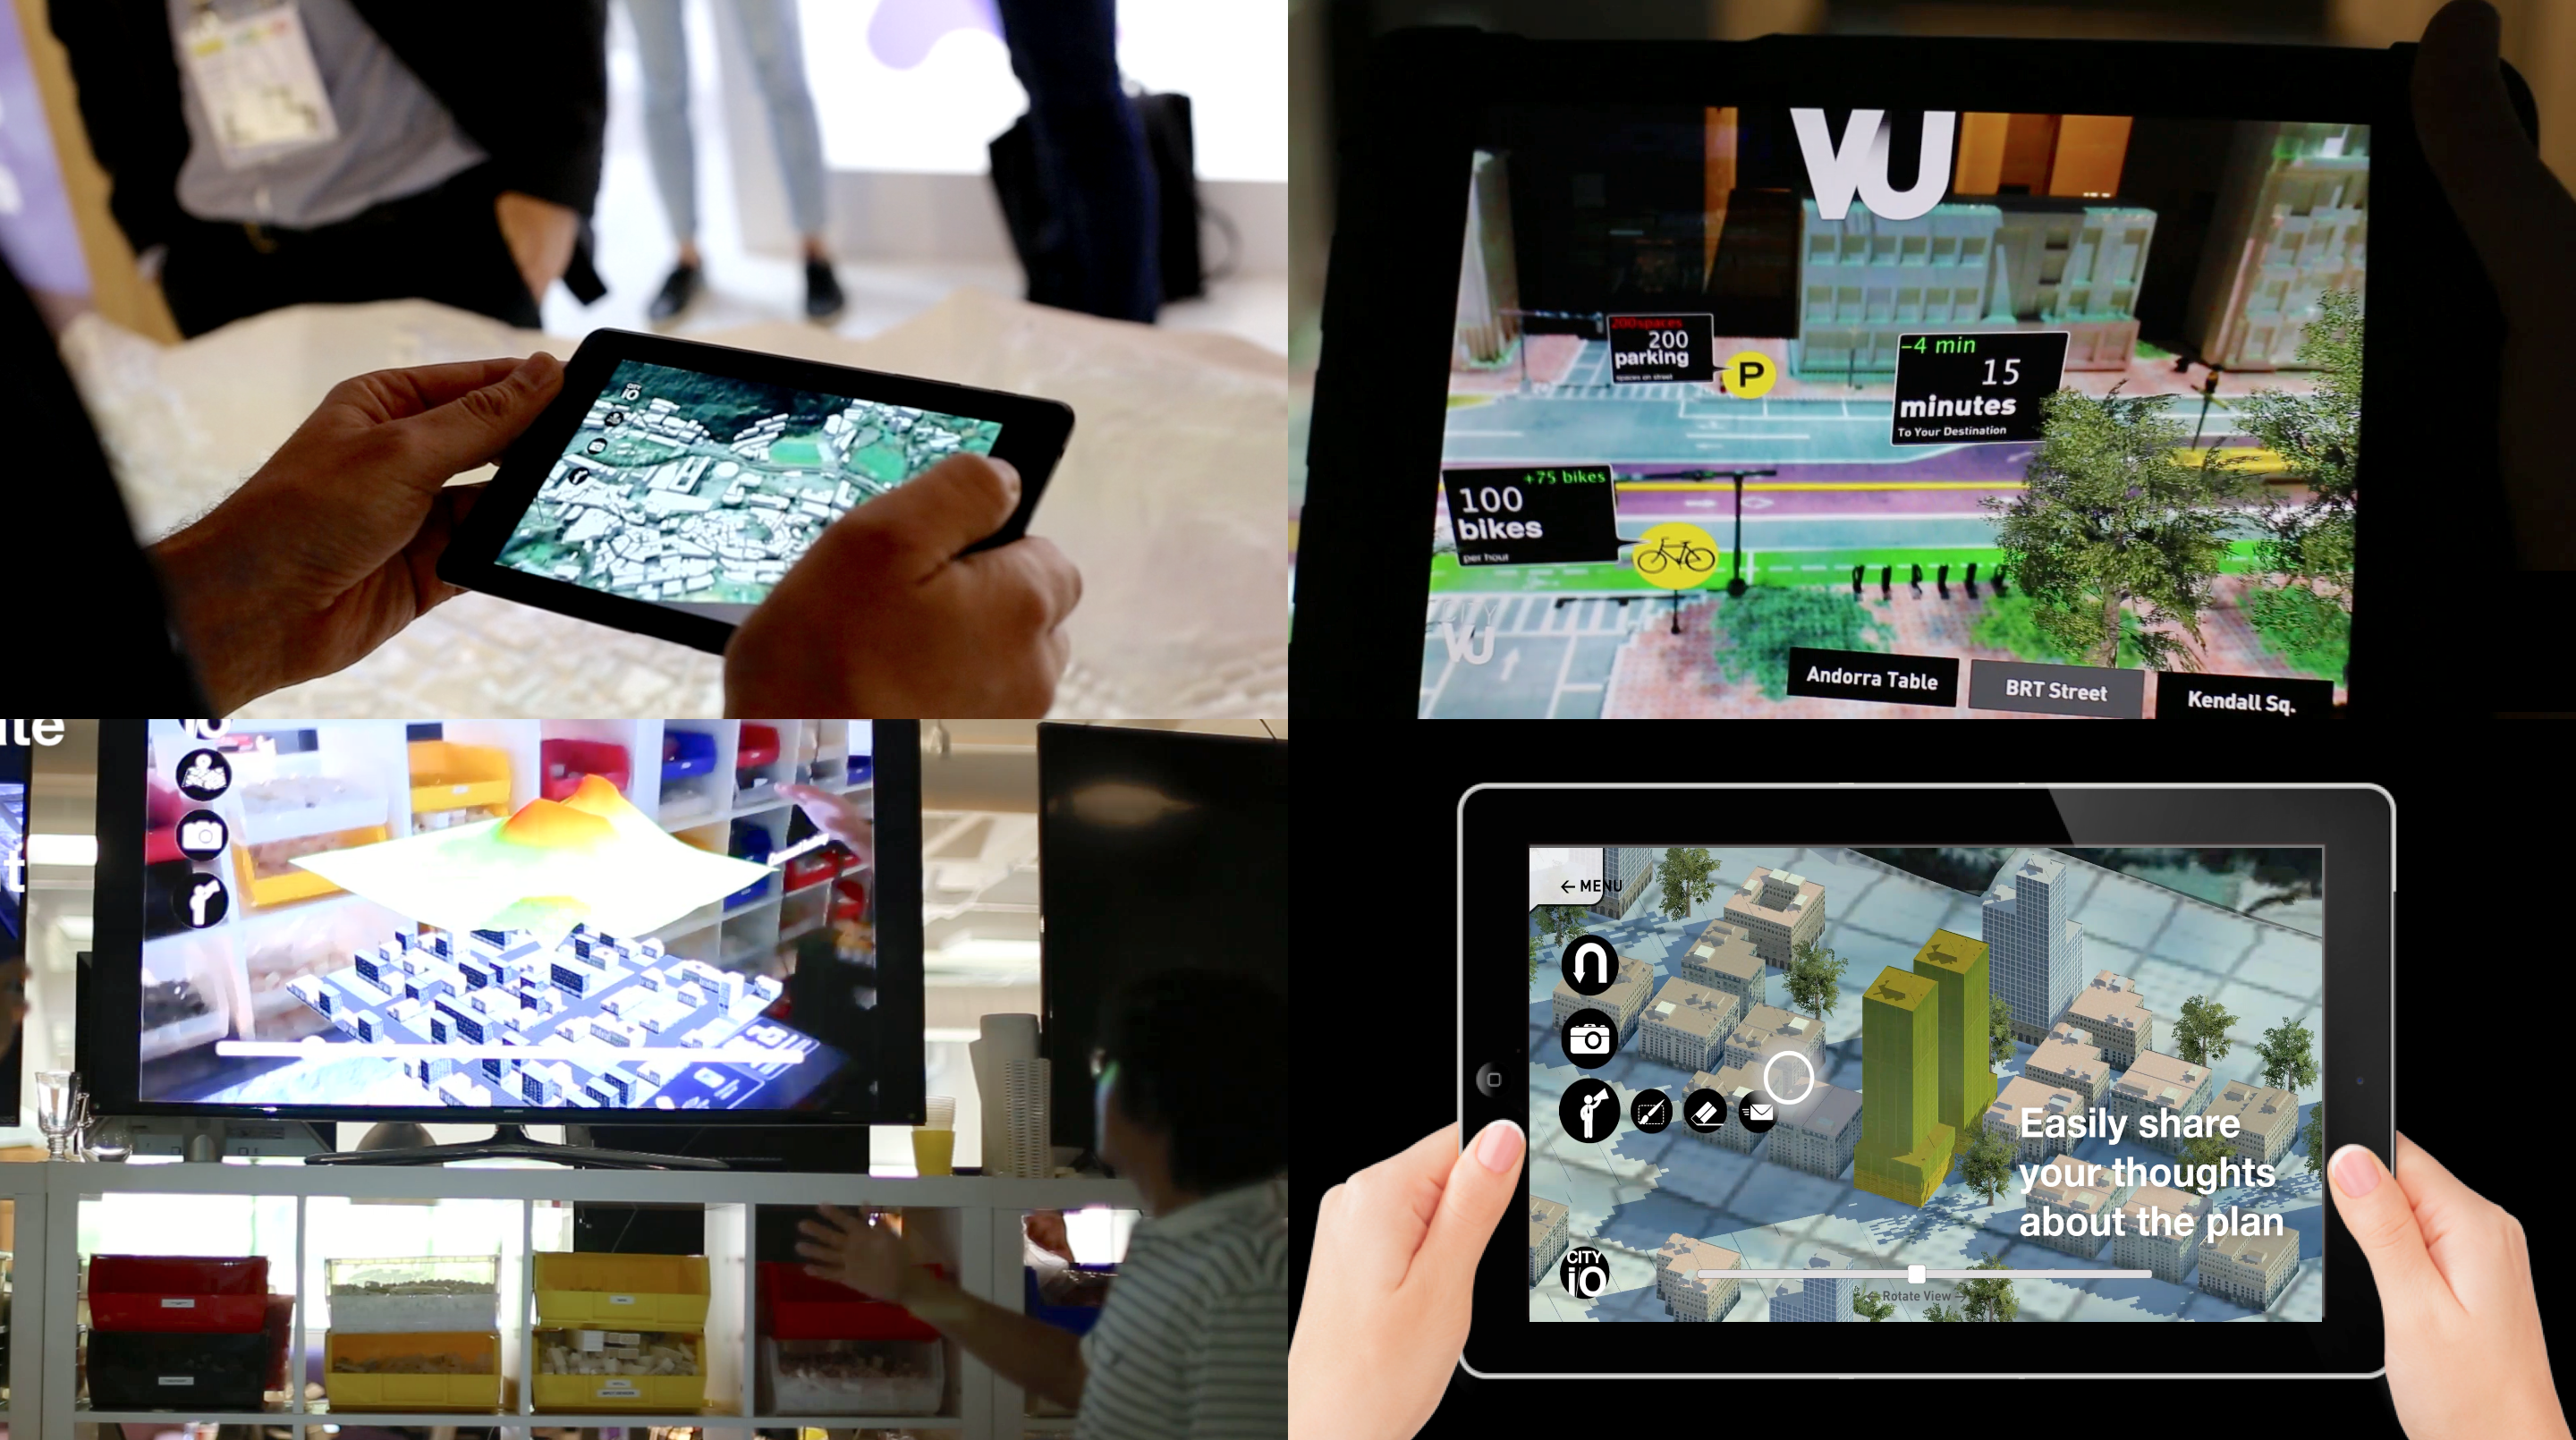
\includegraphics[width=1\textwidth]{chapters/transformation/cs_arch/figures/ar/ar_0.png}
              \end{center}
              \caption{CityScopeAR use-cases. (top-left) Andorra, in the Smart Cities conference, Barcelona \eqref{sec:andorra-data-observatory} ; (top-right) Boston BRT \eqref{sec:brt}; (bottom-left) Real-time interaction analysis with the TUI as a 3D heatmap; (bottom-right) Commenting interface for public engagement.}
              \label{fig:csar_world}
          \end{figure}


          \textbf{AndorrAR:} In 2016, a version of CityScopeAR was developed as part of a research collaboration in Andorra. Nicknamed `AnodrrAR', this variant was deployed at the Smart Cities conference in Barcelona, and later was set on permanent display at the Innovation Space in Caldea, Andorra la-Vella. AnodrrAR was designed as part of an interactive CityScope model which depicted several data layers: (i) Satellite imagery, 3D model of Andorra's landscape and urban areas designated for redevelopment; (ii) cell towers location, and simulation of the population interpreted from CDR data (see \eqref{sec:andorra-data-observatory}); (iii) interactive design proposals for the downtown area, collected from CityScope TUI via cityIO (see Section \eqref{subsec:csarch-cityio}). In this version, users could position and scale master-plans onto geo-located anchors in the virtual city model; and (iv) feedback system, allowing users to comment on urban developments using a virtual `Speech Bubble' interface.
          \newline
          During the Smart Cities conference in Barcelona, hundreds of visitors interacted with the tools, and over 200 feedback comments were recorded during each day of the event. Similar versions of CityScopeAR were deployed in Hamburg at the HCU university (`16), Volpe redevelopment site in Cambridge (`17) and in Shanghai, Tongji University (`17).
      }

      \subsubsection{CityScopeAR: Discussion}
      {
          CityScopeAR extends the CityScope process in terms of scale and location. It retains a linkage to the CityScope tangible interface, while augmenting it with on-demand data, analysis, and feedback. The feedback mechanism added a new layer to the CityScope ecosystem, allowing users to comment on urban development proposals, in a shared virtual or physical design session.
          \newline
          Despite its potential, AR technology is still relatively new, and has yet to reach mainstream usage \cite{mekni2014augmented}. CityScopeAR was an preliminary step towards adoption of AR technology for urban-design, but it also highlighted the challenges of the current state of the art. Specifically, cultivating a collaborative design process using individually hand-held devices was found to be a challenge. A major advantage of the CityScope TUI is in its ability to serve a common ground for conversation and feedback, unobstructed by devices. At the time of writing, even the most advanced AR or VR systems are still struggling with ease of use, accessability, comfort, and performance, hindering their mass use in a collaborative public setting.
      }
  }

  \subsection{Discussion}
  {

      This section discussed the various components of the CityScope ecosystem. It explored the CityScope Schema, a data structure and a standard used across the platform. It detailed the three main components of CityScope: (i) Input and interaction, (ii) urban analysis microservices, and (iii) feedback and visualizations. As a design decision, only few aspects of the CityScope ecosystem are immutable and fixed; Instead, the majority of the ecosystem is designed to be flexible and adaptable to the unique needs of the CityScope community, such as supporting a wide range of urban analytics modules, or the development of different input, visualization, and feedback modalities. The rest of this Chapter shows how this ecosystem was utilized in key CityScope projects.
  }
 }

    %%%%%%%%%%%%%%%%%%%%%%%%%%%%%%%%%%%%%%%%%%%%%%%%%%
    \section{CityScope Playground}\label{sec:cityscope_playground}

{
    \subsection{Introduction}
    {
        In complex decision-making processes, stakeholders from varying backgrounds and expertise are involved. The existing frameworks for city-planning are often designed around certain professional audiences (e.g., planners and architects) and are usually less accessible to a wider scope of users \cite{ben-joseph2001}. A collaborative interactive system could facilitate stakeholder dialogues and interactions, and consequently help them make more informative decisions in shorter time.
        \newline
        This work examines user engagement and decision-making in the context of urban-regulations and zoning. The objectives of this study are twofold: (i) to examine user interactions with tangible user interfaces for urban-planning, and (ii) to investigate stakeholders' engagement and decision-making using these tools.
        This observational study was conducted with a representative sample of users from different backgrounds. These were invited to examine the usability of a CityScope variant developed in 2015, called `Playground'. A comparative analysis of different approaches examined the users' interaction and decision-making using CityScope, in comparison to traditional planning aids. The sessions involved decision-making scenarios using paper-based planning documents, alongside an interactive tangible models of the design area. A coding scheme was developed for analyzing video observations, to examine the wide spectrum of actions, verbal cues, and non-verbal gestures, and quantify the occurrences of these interactions during the experiment.
    }

    \begin{figure}[!htb]
        \begin{center}
            \includegraphics[width=1\textwidth]{chapters/transformation/playground/figures/playground.jpeg}
        \end{center}
        \caption{Impact of zoning-codes and building regulations on urban form. (top) Hugh Ferriss's drawings of NYC 1916 Zoning Ordinance (1922), the first in the United States to regulate building use, floor area, and height of new buildings. (bottom) The effect of zoning on built form and function in Midtown Manhattan.}
        \label{fig:pg_nyc}
    \end{figure}

    \subsubsection{Evaluating UHCI}
    {
        Technologies to support stakeholders in the decision-making process have evolved over the past few decades (see Chapter \eqref{chapter:introduction}). Intuitive tools can create collaborative interaction spaces, where users efficiently work with each other and see the result of their interaction immediately \cite{ishii2002augmented}. Nevertheless, studying the usability and efficiency of such systems is relatively unexplored \cite{Innes2016}.
        \newline
        Several observational studies have been conducted on TUI. Brereton and McGarry \cite{brereton2000observational} tested the usability of tangible objects, and how TUI encourages engineers' design thinking and communication. Fjeld and Sissel \cite{fjeld2002alternative} tested the usability of TUI compared to alternative traditional 3D and 2D single user tools, by examining the learning effect and the overall user experience. These studies showed that 3D tools outperformed in terms of user satisfaction. Falcao and Price \cite{price2009effect} focused on investigating collaborative activities in a tangible table-top environment, to support how shared interfaces affect the way collaborative activities are structured, and examines the kinds of interactions that are productive for learning. Ben-Joseph examined the Luminous Planning Table (LPT) \cite{ben-joseph2001}, in order to further develop its functionality based on feedback from end-users through implementation of an actual parcel slated for development.
        \newline
        This observational study examines the usability of CityScope in a simulated urban-planning process, and investigates its effect on stakeholders' engagement and decision-making. The study aimed to improve the understanding of how a mixture of TUI and virtual environments might encourage collaboration and communication among stakeholders, and lead to better decision making.
    }

    \subsubsection{Kendall Square: Site and Context}
    {
        The study examined user engagement in the context of an early stage city-planning. At this stage, zoning-laws and building-regulations are leading many of the design decisions, and are responsible to the creation of `zoning envelopes': legal frameworks to which the development of new buildings and landscapes is bounded \cite{n15, Ben-Joseph2004}. The preliminary stage of most planning processes is a comprehensive understanding of the spatial and regulatory context. Figure \eqref{fig:pg_nyc} shows the impact of zoning on urban form in NYC.

        \begin{figure}[!htb]
            \begin{center}
                \includegraphics[width=.75\textwidth]{chapters/transformation/playground/figures/playground0.png}
            \end{center}
            \caption{Kendall Square and MIT east-campus. CityScope Playground was used in this observational study to investigate the usability of the TRP system in the context of the MIT east-campus redevelopment project (photo: MIT).}
            \label{fig:pg_kendall_site}
        \end{figure}

        \textbf{Site:} Kendall Sq. in Cambridge, MA, was chosen for this case study. The unique features of this area\footnote{Kendall Sq. is sitting on the verge of MIT, has adjacency to low-density, low-income neighborhoods, close to Boston CBD, and surrounded by unique geographical features.} creates additional interest for the study of regulatory frameworks and their impact on new development (see Figure \eqref{fig:pg_kendall_site} for the redevelopment site used in this study). During the past few decades, the post-industrial area of Kendall Sq. reemerged as a technological hub. Several planning effort were initiated to increase capacity for MIT eastern campus and the adjacent area, aiming to update current height limits, AOR, GFA and other regulations\footnote{See Appendix \eqref{appendix:playground} for the history and a list of redevelopment efforts in the Kendall area.}.
        \newline
        \textbf{Zoning and Regulation:} Kendall Square was intensively planned over the years. Due to its history, location, and unique geography, the site intersects multiple zoning areas. From the south-east, the MIT main campus has mostly low-rise buildings and continuous facades, stretching along Main street and Memorial drive; From the north, a mixture of high-rise office towers, medium-rise condominiums, and low post-industrial structures; In the north-west, low-rise and residential buildings. Over the years, these typologies created a massive trail of zoning and regulations, which can be challenging to distill even by professionals\footnote{An example of this ambiguity could be found in the K2C2 study (Kendall and Central squares), commissioned by the city in early 2011 in response to interest in increased development capacity. Although the study guidelines represent thorough research done in order to improve redevelopment efforts, the legal status of these recommendations is unclear: \begin{quotation} ``The Kendall Square Design Guidelines are created... to \textbf{inform} property owners, business owners, developers, and the general public about the desired form and character of development in Kendall Square...However, the guidelines are not intended to impose a strict limitation on the building form and style. Other creative design solutions, or measures, not noted here may also be utilized to achieve the same goals at the discretion of the Planning Board..." \end{quotation}}.
    }

    \subsection{Tangible Regulation Platform}

    {
        This user study compares two different urban-planning methodologies: (i) Classic, `pen-and-paper' decision-making, and (ii) A digital-physical decision support system. The comparison is meant to enhance the differences between an evidence-based urban-planning session, and a traditional one.
        The Tangible Regulation Platform (TRP) is a CityScope variant designed to evaluate urban-design proposals in the context of zoning-laws and regulations. Users input is examined in real-time, to reflect their impact on the built environment, and to offer an early assessment of the buildable zoning envelopes. For example, a community undergoing a redevelopment initiative, could benefit from the TRP to preform zoning simulation, sometimes years before actual development is taking place. Figure \eqref{fig:pg_trp} shows the TRP setup and usage.
        \newline
        The TRP is composed out of three components: (i) A physical 3D urban model, (ii) a computational unit, and (iii) a feedback module. The computational unit is responsible for evaluating the city regulations and guidelines in response to users input. These algorithms compile zoning, code, and regulations into virtual envelopes, mimicking to the way a municipal board would evaluate a development proposal. Figure \eqref{fig:pg_module} describe the zoning simulation module.
    }

    \begin{figure}[!htb]
        \begin{center}
            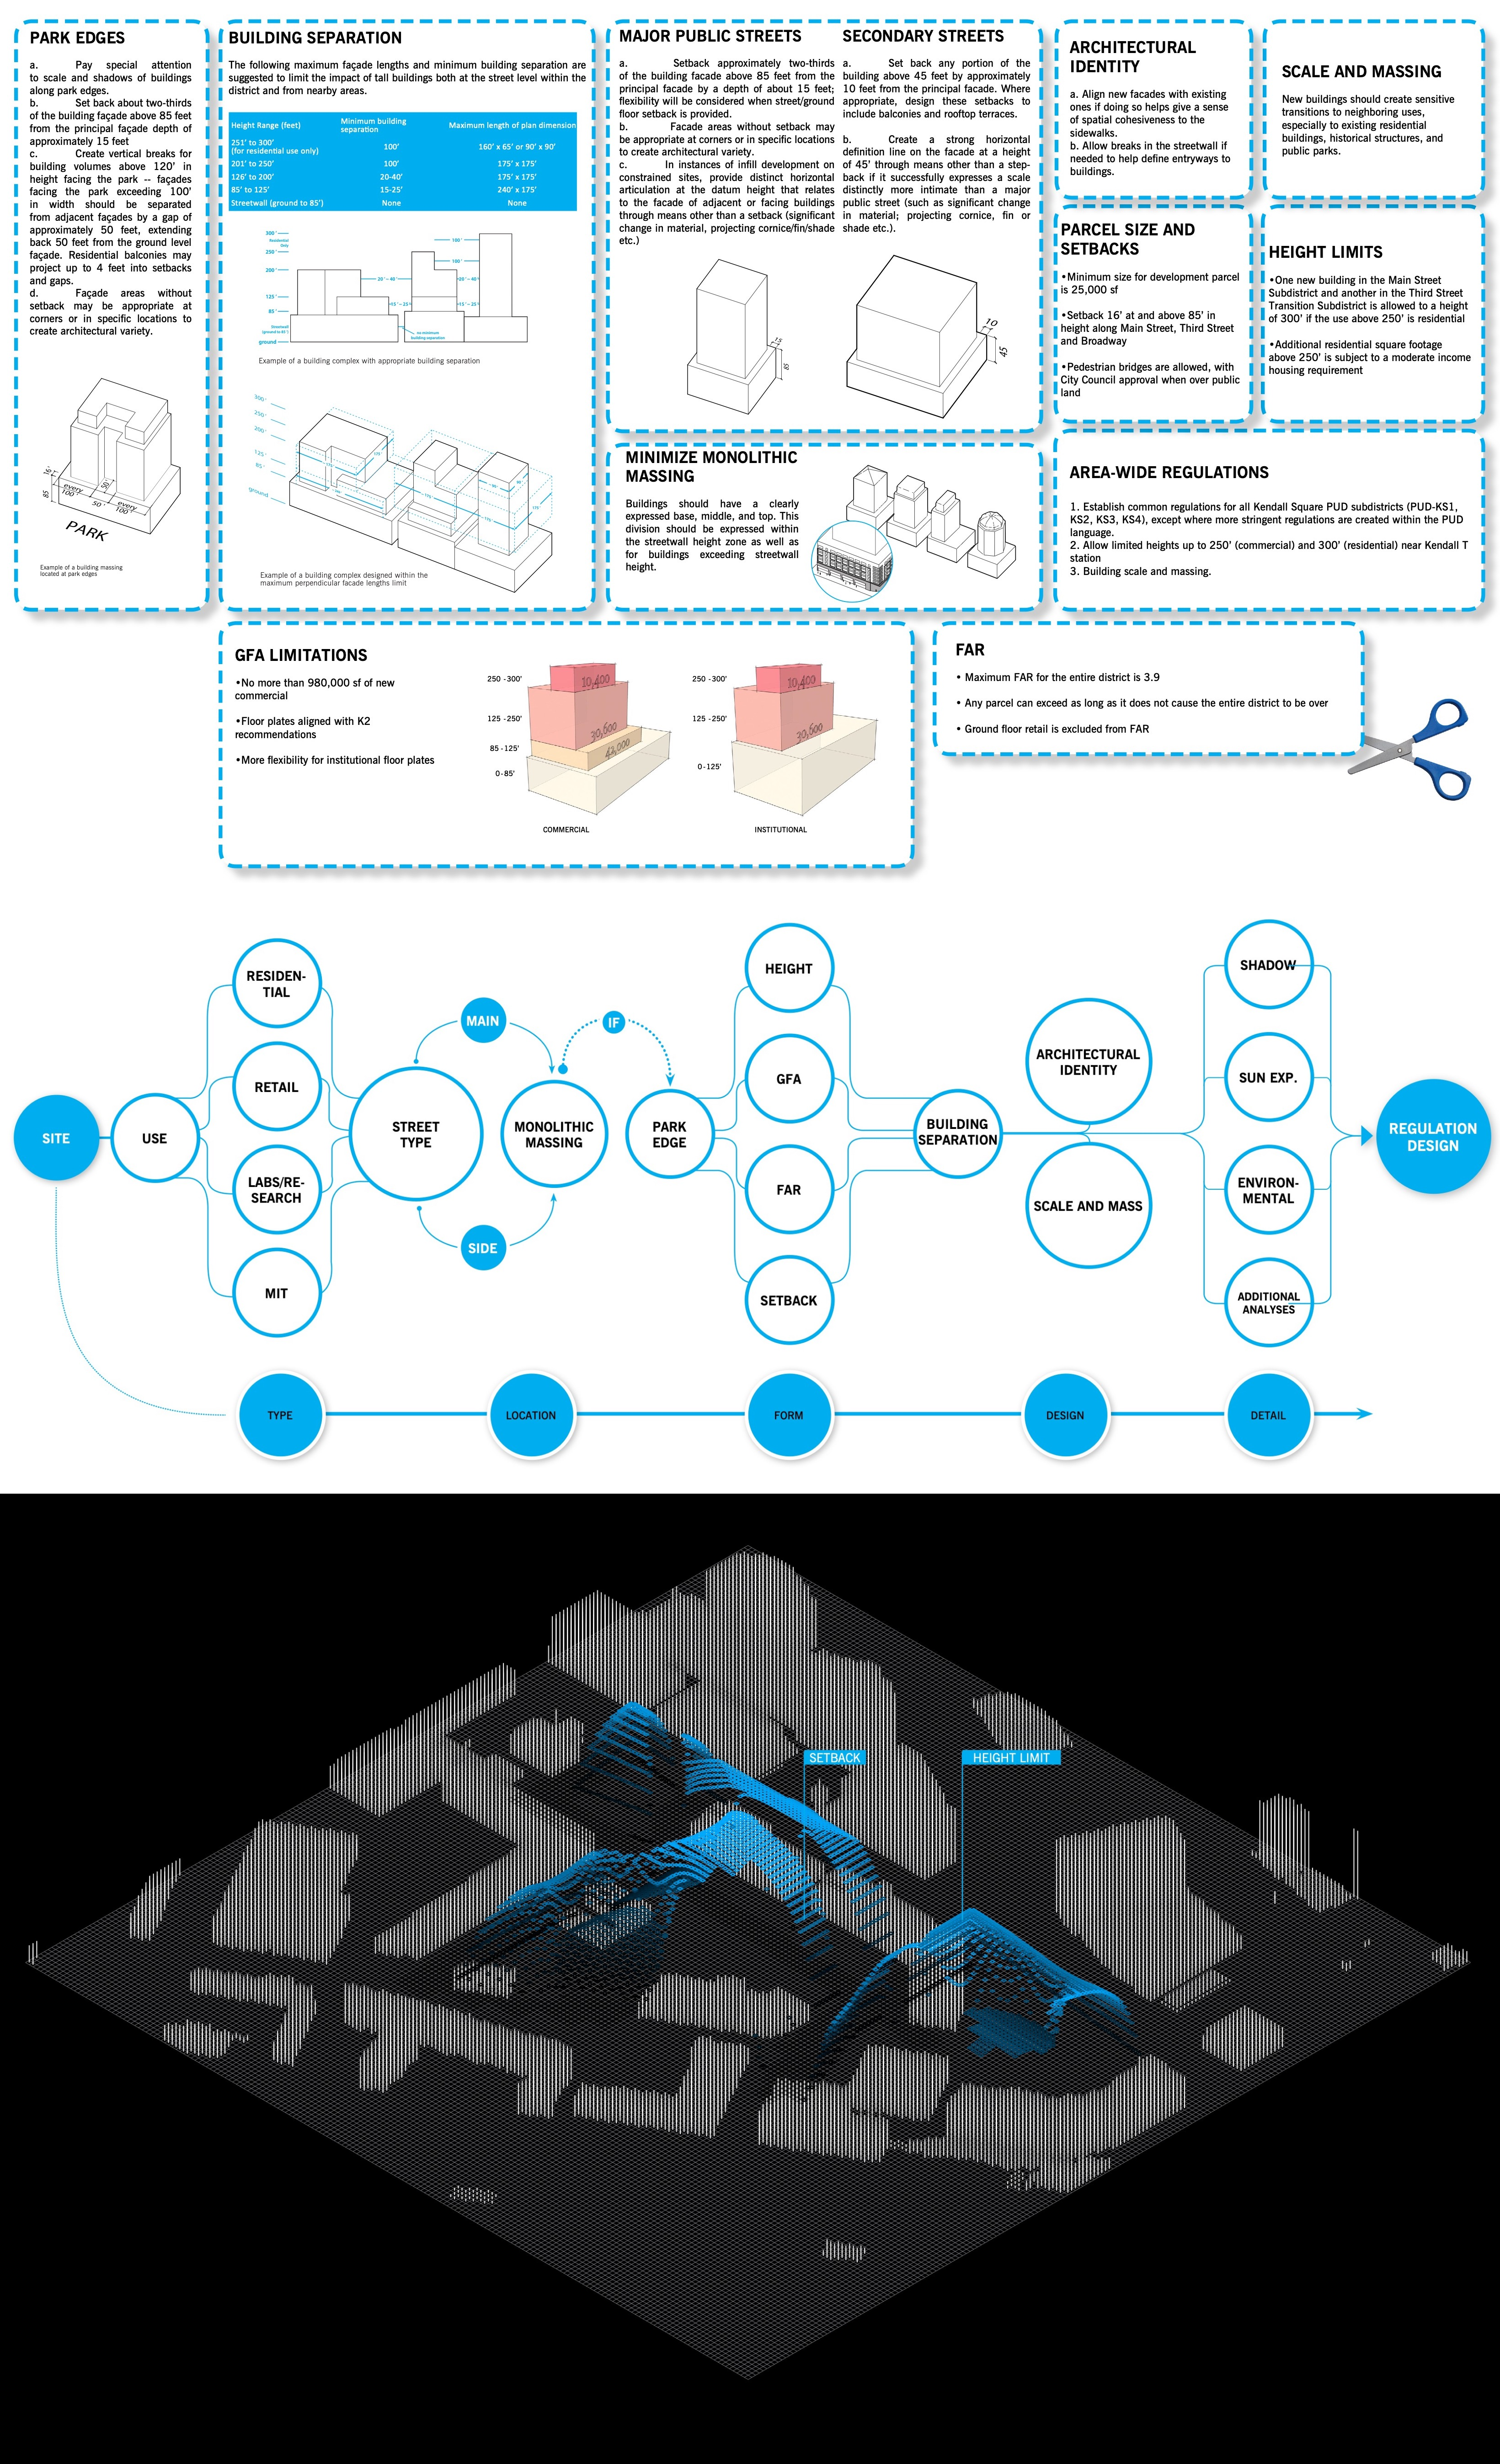
\includegraphics[width=0.65\textwidth]{chapters/transformation/playground/figures/playground2.png}
        \end{center}
        \caption{The `zoning simulator'. (from the top) A subset of the zoning amendments proposed for this site was used for modelling the TRP. The zoning codes and building regulations were converted to logical methods (center), and then linked to other methods to evaluate each design proposal. Finally, the results of the simulation was visualized (bottom).}
        \label{fig:pg_module}
    \end{figure}

    \subsubsection{The TRP TUI}
    {
        The TRP includes (i) an array of tagged 3D objects, serving as massing elements of zoning envelopes, (ii) a table that constrains the placement of 3D objects into an urban context, (iii) sensors for scanning the scene, computers, display screens, and projectors for projecting light patterns onto the table. The TRP tabletop is composed of a physical grid of 192x192 LEGO bricks; The grid represents two conditions: (i) `fixed': the non-modifiable parts of the city, and (ii) the `playground': the interactive part of the TRP. A user places physical objects into indentations which form a grid on the table; The objects are then scanned and digitally reconstructed (see Section \eqref{subsec:csarch-cityscopy} for technical description of scanning and parsing the table's state).
        \newline
        Similar to digital monitors, the `resolution' of the table - the density of pixels for a given area - is a key parameter which dictates interaction, simulation, and feedback. Unlike meticulously crafted urban maquettes, the `roughness' of the pixelated CityScope model is intentionally shifting the focus from design details to the overall scheme, massing, and relationships between functions.
        When designing the platform, the smallest tile should represent the smallest unit of interaction and analysis. This decision stems not only from the physical aspects of the urban context, but also from the smallest analytical unit. In the case of the TRP platform, this measurement was based on the smallest unit being used in the site's zoning documents, equal to ~8ft\footnote{The smallest unit was found in an 8ft setback rule, imposed on low-rise building parcels of side streets. This rule was set as the smallest sampling unit for the entire urban model and consequently - for the buildings' height and appearance.}.
    }

    \subsubsection{Types System}\label{subsec:playground_types_system}

    {
        A set of rectangular blocks was defined as the `Bank'. The blocks, different in height but equal in their footprint, are a collection of 16 unique `zoning elements'. Each element retains two parameters: land-use and height, and each block can hold more than one land-use; For example, one block with 22 floors may include 3 floors of retail space in the street level, and 19 floors of residential or office space above. Here, a single block cannot represent a building; In order to construct a viable building envelope, each of the given blocks must be attached to others. The assemblage of these blocks creates zoning envelopes that are diverse in size and program, thus creating a complex zoning environment\footnote{CityScope Playground used an early data scheme to represent the table's state and interaction. For the CityScope Schema, see Section \eqref{sec:cityscope_architecture}.}.
    }

    \subsubsection{Feedback Module}

    {
        \textbf{Scanning And Evaluation:} When users change the configuration of the 3D objects array, the digital reconstruction of the CityScope grid is analysed in relations to the zoning and regulation. The output of this analysis is plotted as a visualization to both the tabletop and a set of vertical monitors. The users then react to the feedback in their next interaction with the TRP.
        \newline
        \textbf{Feedback Devices:} The TUI setup consists of two output devices: Array of 4 projectors, mounted to the room's ceiling above the table corners; The projectors are synced to the 3D models shape using projection mapping. The projectors display data visualization corresponding to users` interaction, so that changes made to the physical model will be visually echoed.
        The second part of the feedback module is a TV dashboard, synced with the projected visualization. Information displayed on the screen is (i) GFA calculation for new additions and for existing urban context; (ii) Percentage of buildings using or exceeding existing FAR; (iii) Open space and built-area ratios; (iv) Occupancy and sub-sectioning of each land-use.

    }

    \subsection{Observational Study}

    {
        The observational study was conducted with a representative sample of users from different backgrounds. The users were randomly invited to examine the usability of the TRP, and to express their opinion on ways to improve planning processes through such platforms. The sessions involved decision-making and design scenarios using artifacts such as paper-based sketching, note-taking, as well as verbal discussions. All sessions were recorded and analyzed; A coding scheme was developed for analyzing the video observations, in order to examine the wide spectrum of actions, verbal cues, and non-verbal gestures, as well as quantify the occurrences of these interactions during the experiment.


        \begin{figure}[!htb]
            \begin{center}
                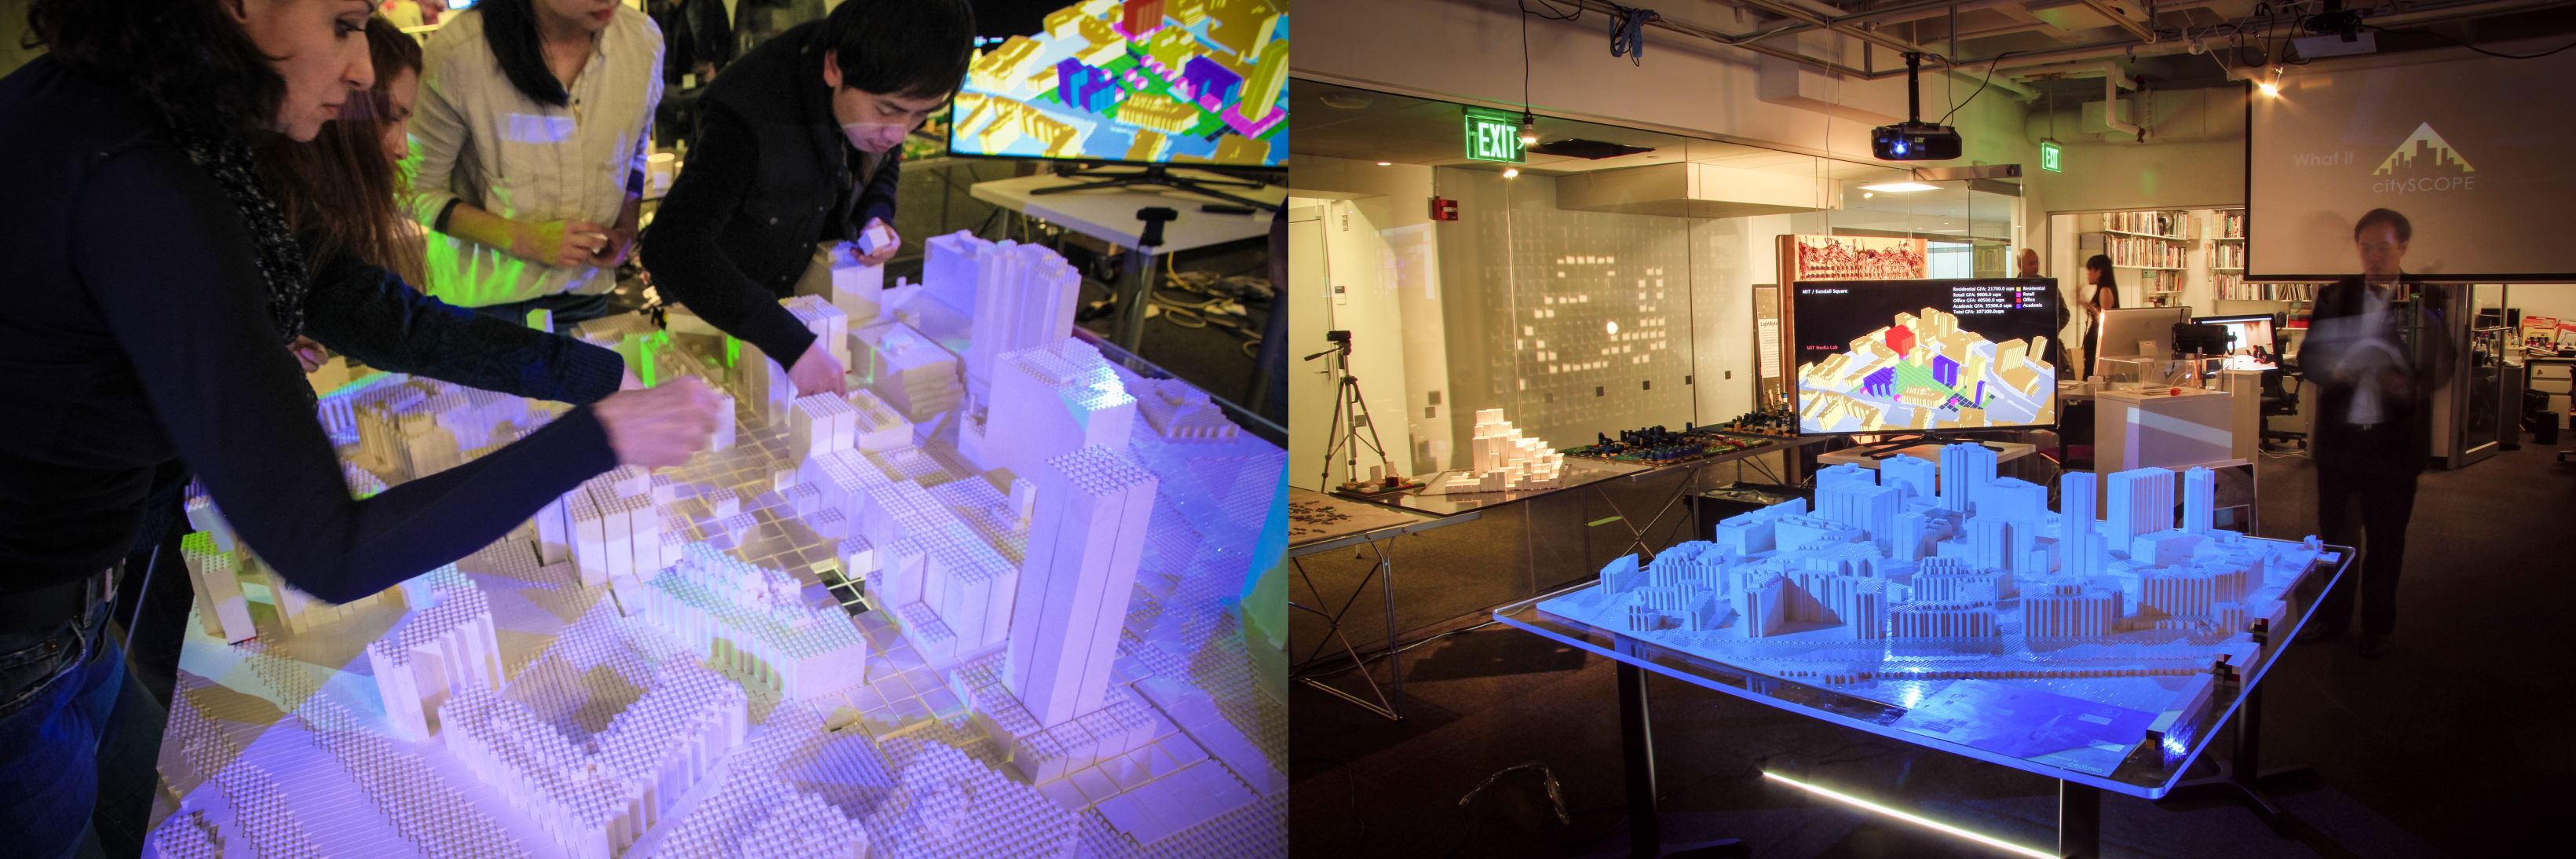
\includegraphics[width=1\textwidth]{chapters/transformation/playground/figures/playground1.png}
            \end{center}
            \caption{CityScope Playground and the TRP. (right) Overview of the complete system, including the TUI, feedback module, and the `Bank'. (left) The TUI in use during the experiment. Users can collaboratively interact, discuss, and improve their design based on feedback from their peers and the system's responses.}
            \label{fig:pg_trp}
        \end{figure}

        Fifteen participants from the MIT community, including students, staff, and affiliates were invited through an open, unrestricted online form, email lists, and in-campus publications. Upon arrival, the participants were divided into two groups: \textbf{Community Meeting session:} This group held a paper-based discussion, and later moved to the \textbf{TRP session:} In which participants were invited to use the interactive tangible model.  Recording was done using Morae \cite{techsmit94:online}, a usability testing tool to record and analyze multiparty sessions.


        \subsubsection{Procedure}
        {
            In each of the sessions, participants were asked to respond to real-life planning and design challenges in the Kendall Sq. area. At the beginning of the day, the groups were informed about past and existing master-plans and zoning restrictions imposed on the site. They were then asked to rebuild and plan the Kendall Sq. area, taking into account zoning restrictions by adding residential, commercial buildings, parking lots, parks and public amenities. In the TRP session, participants were asked to do the same, while interacting with the CityScope platform. The TRP real-time feedback notified the user whenever a violation of the zoning restrictions occurs in their design, through visualization, text, and symbols.
        }




        \begin{figure}[!htb]
            \begin{center}
                \includegraphics[width=1\textwidth]{chapters/transformation/playground/figures/playground3.png}
            \end{center}
            \caption{User interaction and TRP feedback. As users interact with the TRP, the system evaluates the design based on the zoning simulator module. As users progress with their spatial design, the system highlights violations of the zoning-laws and building-codes, allowing the user to align their design or otherwise challenge the zoning rules.}
            \label{fig:pg_interaction}
        \end{figure}


        \subsubsection{Analysis}

        {
            The video recordings of the sessions were analyzed using a coding scheme. The different types of coding schemes, actions, verbal and non-verbal behaviors are described in Table \eqref{tab:coding_scheme}; Results of the analysis are presented in the Appendix Table \eqref{appendix:coding_scheme_results}.

            \begin{table}
                \begin{center}
                    \caption{Coding Schemes}
                    \label{tab:coding_scheme}
                    \begin{tabular}{l|ll|ll}
                        Code & Description           & Code & Description                              & \\

                        \noalign{\hrule height 0.5pt}

                        EXP  & Explore Function/Tool & EXT  & Excitement                               & \\
                        PUZ  & Puzzled               & SUR  & Surprised                                & \\
                        CLA  & Clarification of Idea & ACT  & Wrong Action                             & \\
                        IDE  & Introduction of Idea  & FRT  & Frustration                              & \\
                        ACC  & Acceptance of Idea    & DIS  & Discontinuous Action                     & \\
                        EVA  & Evaluation of Idea    & REC  & Recognition of Error or Misunderstanding & \\
                        REF  & Refinement of Idea    & DBT  & Doubt                                    & \\
                        HAN  & Hand over             & COR  & Corrective Action                        & \\
                        HES  & Hesitation            & FLO  & Floor-Holding                            & \\
                        DIF  & Execution Difficulty  & TAS  & Give Task to Another User                & \\
                        EXE  & Execution Problem     & SCH  & Search for Non-Existing Function         &
                    \end{tabular}
                \end{center}
            \end{table}
        }
    }

    \subsection{Results and Findings}

    {
        The video recordings of each session was analyzed using the predetermined coding scheme. This scheme included several types of actions, verbal and non-verbal behaviors, and physical gestures. The coding scheme helped recognizing behavioral patterns in the different sessions. For example, it was apparent that most participants spend the first part of their session exploring the TRP and searching its basic functionality, as noted by the multiple occurrences of $EXP$ and $SCH$ codes. Therefore, it can be assumed that a demonstration of the system would make users more comfortable interacting with it. The occurrences of code $IDE$ indicates that dealing with physical objects made participants more active and engaged in the planning and decision-making process. The $ACC$ code reflects that due to the feedback visualization, participants shared a common understanding of the proposed plan. As indicated in the multiple occurrences of $CLA$ and $EVA$ codes, the attention to zoning violation was greater while using the TRP due to real-time feedback. Unlike traditional sketching methods, where participants might not consider zoning, the TUI assisted participants in identifying violations of the zoning restrictions.
        \newline
        In terms of TUI design, the systems was found to cause some frustration and confusion (which is noted in codes $FRT$ and $PUZ$) when participants could not differentiate between removable and fixed physical objects, and when they indicated difficulties in identifying an object. These observations revealed opportunities for improving the user experience of the TUI system\footnote{For full breakdown of the coding scheme results, see Table \eqref{tab:coding_scheme} in the Appendix.}.
    }


    \subsection{Discussion}
    {
        In order to design successful UHCI systems that supports collaboration and facilitate decision-making between stakeholders, it is essential to test their usability in real-world scenarios.
        This study analyzes the usability of a Tangible Regulation Platform (TRP) system, by applying a coding scheme on recorded observations of users' experience, and decoding them to asses usability, and interaction. These findings suggest that UHCI are superior to traditional urban-planning methods in terms of rapid prototyping, collaboration, and decision-making processes.

        \subsubsection{Strengths}
        {
            The TRP platform had several key technological and operational advancements over prior art: This platform was the first large scale CityScope that incorporated real-time interaction, feedback, and participation, all in one system. Despite analyzing unconventional metric such as zoning laws, the TRP feedback was proven to be effective in user experiments.
        }

        \subsubsection{Challenges}

        {
            Evaluating the platform within the confines of the Media Lab building had several limitations. First, intervention in an existing urban-design proposal should involve stakeholders or communities that have direct relations to the site in question. Amongst the visitors, only few were local residents who generally shared a wide and inconsistent degree of acquaintance with the site.
            Second, the TRP zoning analysis could not be evaluated against the actual process of zoning evaluation by the city. In later CityScope projects, evaluations and analysis would be comparative to the actual evaluation process (for example, see the Grasbrook project \eqref{sec:grasbrook}).
        }

        \subsubsection{Opportunities}
        {
            A key finding emerging from both formal and informal feedback, was that participants desired to not only use the TRP to evaluate zoning, regulations, and building-code, but also to use it for other urban performance metrics. As such, municipalities or public officials may test walkability and transportation concerns; The quality of open landscapes, public amenities and civic safety can be tested in existing or amended regulations; Potential ROI, revenues, or market-appeal of properties can be assessed prior to regulatory amendments.
        }
        \newline
        These findings paved the way to a more holistic approach in the design, development, and deployment of future CityScope platforms. The rest of this Chapter details a unified CityScope platform which is set to answer multiple spatial questions, and to be used by multiple stakeholders, settings, and stages of the planning process (see \eqref{sec:cityscope_architecture}, \eqref{sec:grasbrook}).

    }
}
    %%%%%%%%%%%%%%%%%%%%%%%%%%%%%%%%%%%%%%%%%%%%%%%%%%
    \section{CityScope Volpe}\label{sec:cityscope_volpe}
{
    \subsection{Introduction}

    {
        Building upon the PlayGround-TRP project \eqref{sec:cityscope_playground}, this work extends CityScope with different layers of information and real-time analytics. The urban context for this project was the Volpe site in Cambridge, MA, which in 2016, was still vacant and set for redevelopment. CityScope Volpe was designed to explore the impact of different interventions, both within the site and its surrounding context, with three primary objectives: (i) To communicate complex urban data and the inter-relationships between urban systems; (ii) To simulate the impact of urban interventions; (iii) To support decision making in an iterative process using a tangible interface. Figure \eqref{fig:volpe_overall} shows CityScope Volpe, the TUI, and the real-time metrics.
    }

    \begin{figure}[!htb]
        \begin{center}
            \includegraphics[width=1\linewidth]{chapters/transformation/volpe/figures/volpe0.png}
        \end{center}
        \caption{CityScope Volpe. (left) a set of KPIs and urban indicators are evaluated with each design iteration. (upper-right) The users interactions are translated to three-dimensional zoning envelops, which represent the maximal intervention framework, rather than actual building volumes. (lower-right) Users are presented with both outputs as a mean to direct their design collaboration process.}
        \label{fig:volpe_overall}
    \end{figure}

    \subsection{Site and context}
    {
        As discussed in the previous project \eqref{appendix:playground}, Kendall Sq. was going through extreme urban transformation, driven by the proximity to MIT, Harvard, and the many industries in this area. A limited housing stock and high land values made most residential opportunities in the area out of reach: With a residential density of $\sim$3,000/km$^2$, most workers commute long distances from the greater Boston area, at the cost of energy and time \cite{blanding_blanding_2016}. Additionally, affordable housing incentives were inadequately promoting the necessary range of housing options, and the zoning ordinance has overly restrictive land-use requirements \cite{noyman2015powerstructures}. Alongside low residential density, is the scarcity of services, amenities and 3rd-places, which tend to indicate the urban vitality of a place \cite{Glaeser2011, banerjee2011companion}.
    }

    \subsection{Method} \label{subsec:vople_cityscope}

    {
        CityScope Volpe was built to investigate the redevelopment of the 14-acre DOT facility site, purchased by MIT in 2019 \cite{mit_news}. The physical 3D model is built using LEGO and covers a region of $1km^2$ at a scale of 1:762m\footnote{each 4x4 LEGO tile represents a 26.7 x 26.7 meter area, or 6.675m per LEGO stud.}. Similar to the TRP \eqref{sec:cityscope_playground}, the interactive portion of the model is integrated into the surroundings to represent the area under development, as shown in Figure \eqref{fig:volpe_site}. This intervention region utilizes `CityMatrix' \cite{zhang2017citymatrix}, a Rhino-Grasshopper script \cite{TheHisto40:online} for scanning and virtually reconstructing the interactive site. Interchangeable LEGO tiles represent different land-uses ranging from roads, parks, amenities, residential or office buildings. The TUI also includes physical components with sliders and toggles to change the building height and switch between alternative mobility modes. These modifications are recorded and passed to the computational analysis unit in order to provide real-time feedback to the user. The next section describes the different metric computed by the platform, and the different auxiliary tools and software used to compute them.
    }


    \begin{figure}[!htb]
        \begin{center}
            \includegraphics[width=1\linewidth]{chapters/transformation/volpe/figures/volpe3.jpg}
        \end{center}
        \caption{The DOT Volpe facility site. The redevelopment site is abstracted to the CityScope grid, in which the context is immutable and the site is interactive.}
        \label{fig:volpe_site}
    \end{figure}

    \subsection{Urban Performance Indicators}

    {
        In CityScope Volpe, urban performance is analyzed in terms of social, economic and physical attributes, which are clustered as Density, Diversity, Proximity, Mobility, Building Energy and Innovation Potential \cite{katz2014rise}. The computational analysis uses a number of tools to calculate a range of performance metrics, and produces feedback in the form of both spatial and numerical statistics, including Rhino-Grasshopper, GAMA platform, and Unity \cite{TheHisto40:online, grignard2013gama, UnityRea35:online, noyman2018CityScopeARUD}. The different urban performance indicators are shown in Figure \eqref{fig:volpe_overall}. The rest of this section overviews the different metrics and indicators used in the analysis.

        \subsubsection{Density}
        {
            The ratio between housing, commercial space, retail venues, cultural institutions, and other amenities is known to be related to the creation of well functioning cities \cite{lynch1984good, gehl2013study, katz2014rise}. Density has to be balanced in order to ensure positive outcomes (such as greater exchange of ideas, economic mobility, more employment options, better amenities, or energy reduction) with fewer negative outcomes (such as traffic congestion, lack of natural resources, or pollution) \cite{hawley1972population, UnitedNationsHabitatIII2017, deloitte_2021}. In Volpe, the density of each land-use type (eg. amenities, residences, employment) can be represented as $Density^m=\frac{|M|}{A}$, where $M$ is the set of occurrences of $m$ in the design area, and $A$ is the total area of district.
        }


        \begin{figure}[!htb]
            \begin{center}
                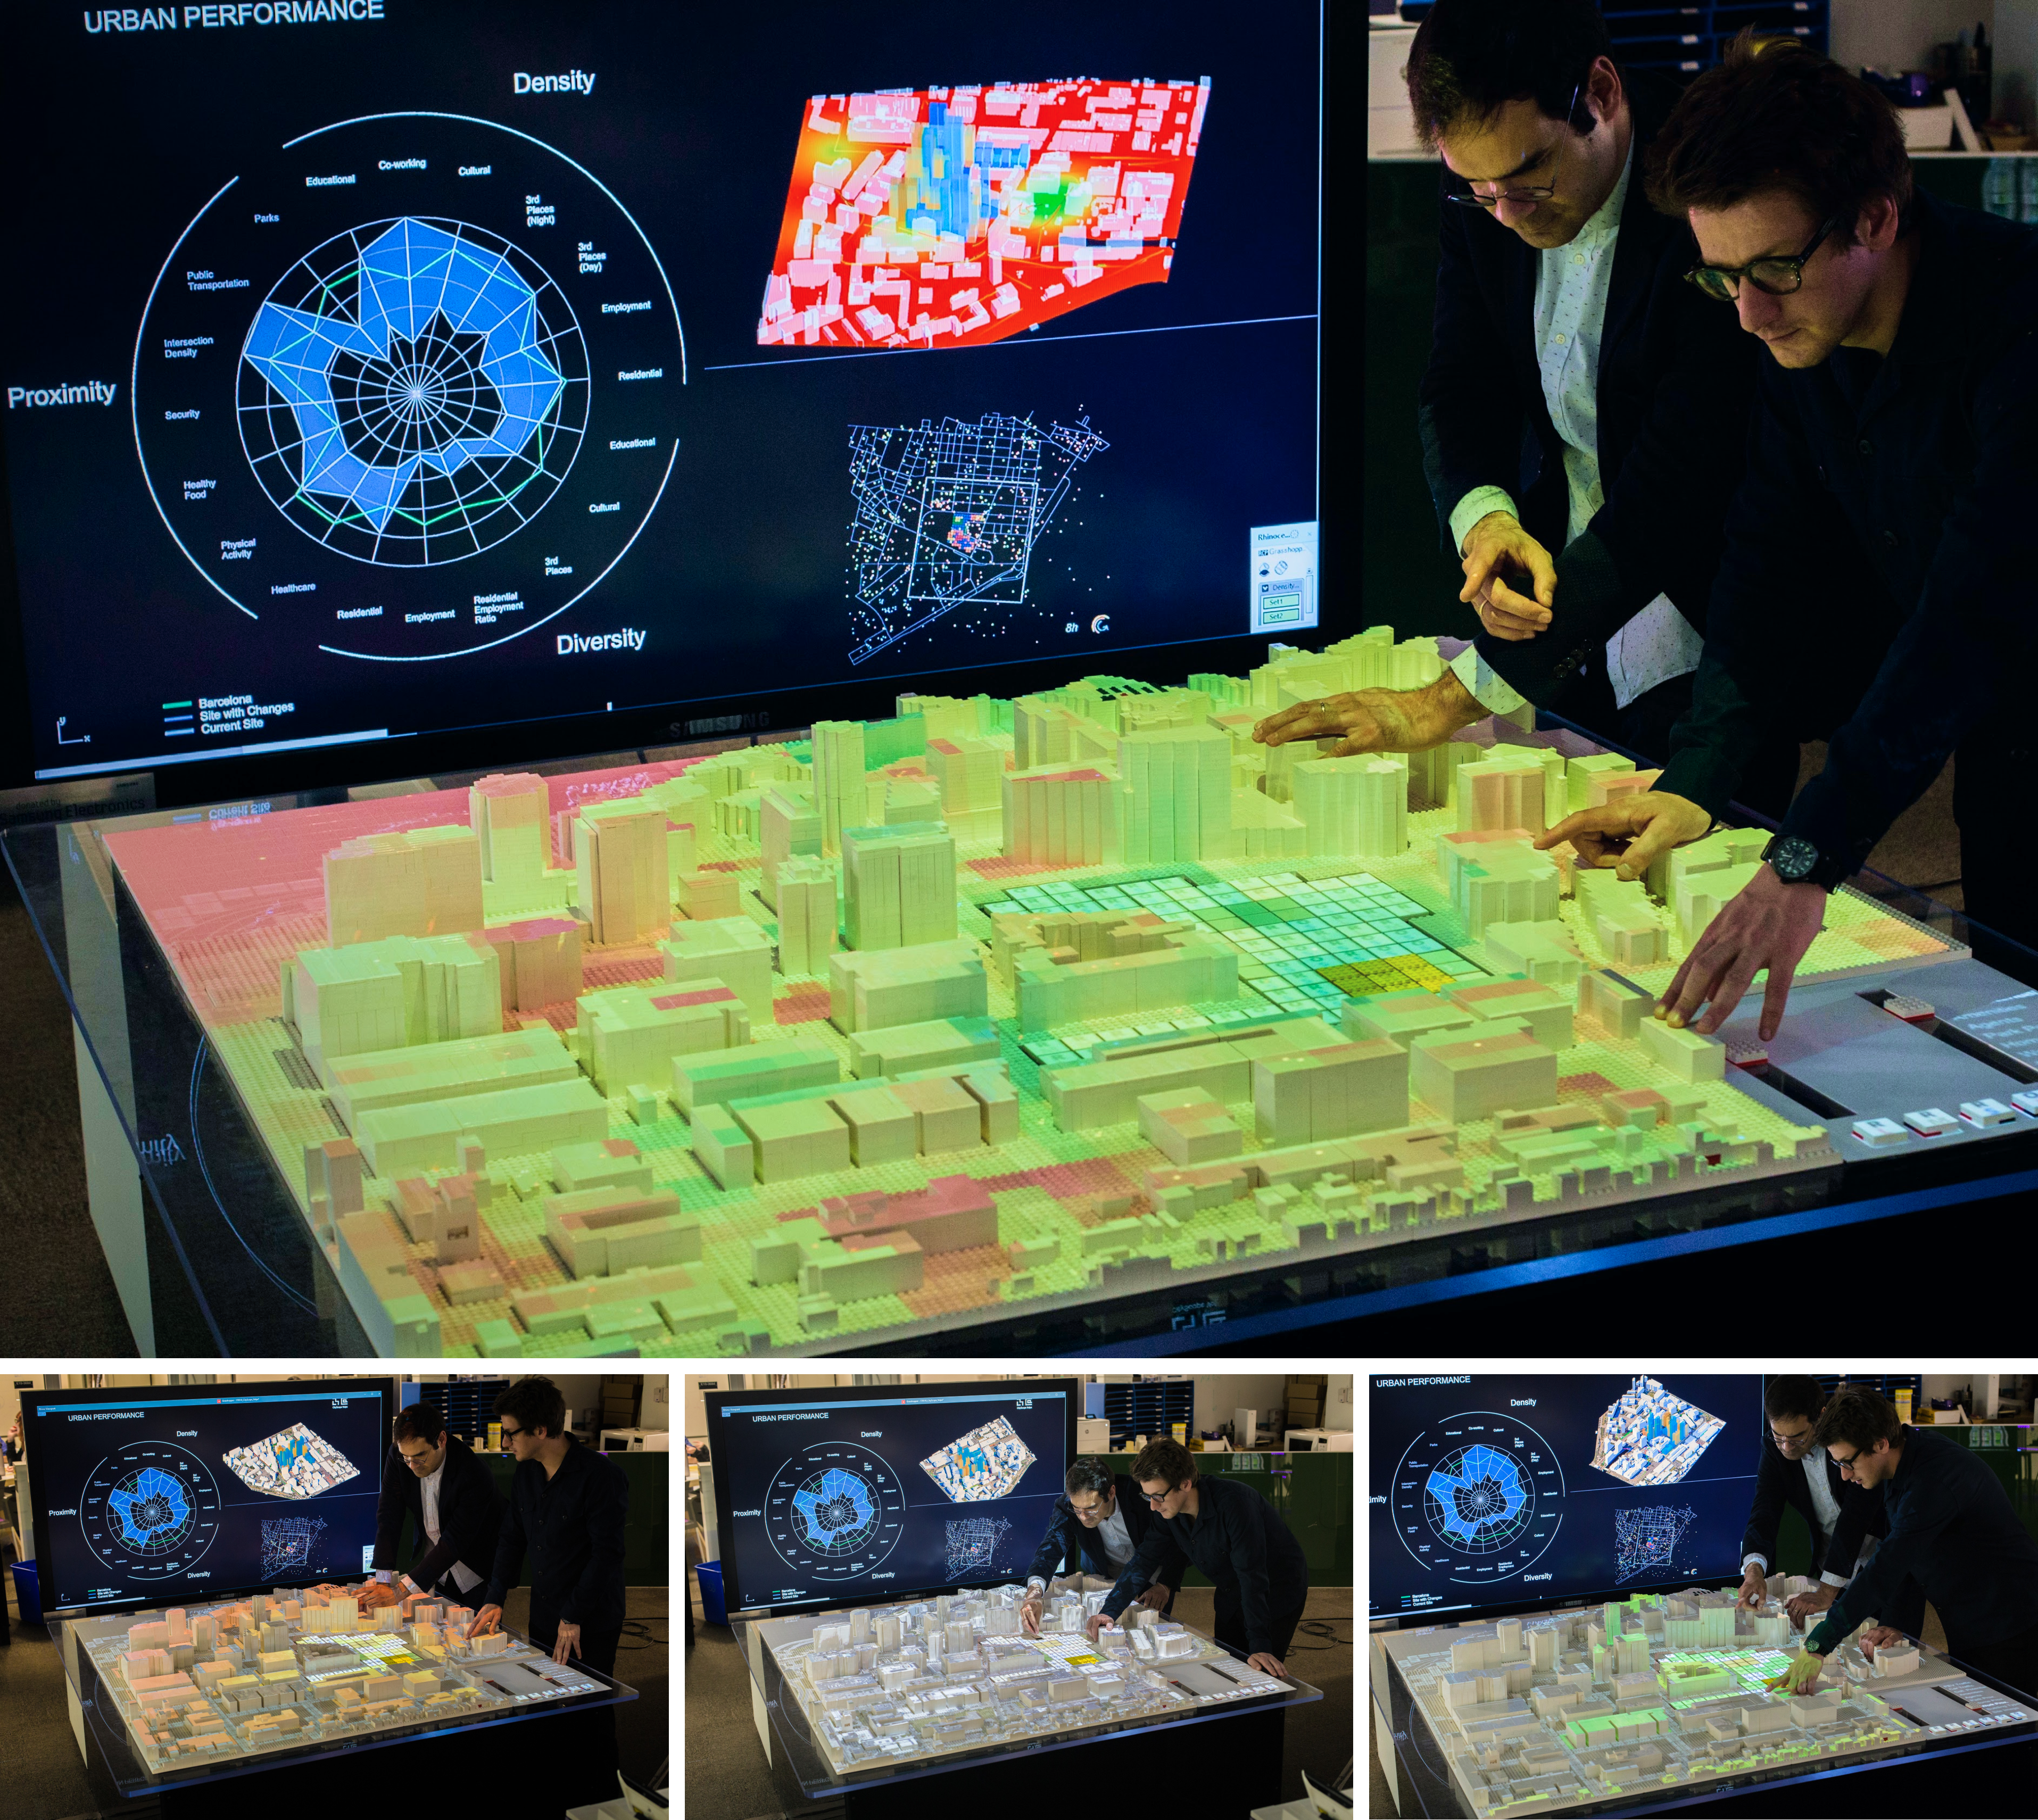
\includegraphics[width=1\linewidth]{chapters/transformation/volpe/figures/volpe2.png}
            \end{center}
            \caption{User interaction and feedback. As users interact with the CityScope TUI, urban performance indicators update in real-time: density, diversity, proximity, mobility energy per person, walkability, access to parks, and a simulated probability of meeting areas (so called `collision potential').}
            \label{fig:volpe_layers}
        \end{figure}

        \subsubsection{Diversity}
        {
            Highly performative urban areas tend to present an increased diversity of social, economic and spatial characteristics. The Diversity index is assessed using a Shannon-Weaver formula \cite{kemeny2013immigrant} and Balanced Ecosystem index: Quantitative measurement that reflects how many different types (species) there are in a certain set (community/ecosystem), and simultaneously takes into account how evenly the basic entities (individuals) are distributed among those types. This can be represented as $H = - \displaystyle\sum_{i=1}^{S} p_i ln p_i$, where $H$ is the Shannon diversity index, $S$ is the total number of species in the community, and $p_i$ is the proportion of the population made up of species $i$. Naturally, not all species are - or should be - equally represented, and the diversity index only measures the distribution of these species.
        }

        \subsubsection{Proximity}

        {
            Proximity assesses the accessibility and closeness indexes between social, economic and physical functions in urban environments \cite{sevtsuk2016pedestrian}. Historically, high performing cities resemble networks of compact urban districts where resources and amenities of daily life are in close proximity to one another \cite{westerink2013dealing}. In Volpe, proximity metrics include walkable access to parks, housing, jobs, mass transit, schools, and amenities. For a given `goal object', a proximity metric for a district can be calculated as $Closeness\,to\,SM = (\sum\limits_{j\epsilon B_i} dist(j,closest(j,SM)))^{-1}$, where $B_i$ is the set of tiles in district $i$, $SM$ is the `goal' objects (Parks, Residential, Office, etc.), $dist (a; b)$ is the geographical distance between two elements' centroids $a$ and $b$, and $closest (j;Y)$ is geographically closest element in set $Y$ from block $j$ centroid. Figure \eqref{fig:volpe_layers}(top) shows the proximity metric for parks in the Volpe site as a heatmap over TUI.
        }

        \subsubsection{Mobility Energy}
        {
            Several mobility metrics are introduced in this project. An Agent Based Model (ABM) simulates a synthetic population in response to changes in land-use and mobility modes, and calculates the energy produces by each trip \cite{grignard2017agent}. The impacts of urban mobility on energy consumption can be calculated as $E_m = \sum_{m \in M}\sum_{l \in L}v_l^m s_{l} e^m$ where $E_m$ is the total mobility energy, $M, L$ is the set of all transport modes and road network links respectively, $v_l^m$ is the number of vehicles of mode $m$ that travel on link $l$, $s_l$ is the length of link $l$, and $e_m$ is the energy usage per unit distance traveled by mode $m$.
        }

        \subsubsection{Building Energy}
        {
            Energy Consumption is calculated for structures in and around the Volpe area using building envelope performance data, orientation, estimated embodied energy, and land-use information. The metric aims to predict how overall energy consumption of the buildings will change given different urban configurations. The model uses a combination of building use, height, and proximity to adjacent structures in order to account for solar gain. The energy efficiency index is found by dividing the total energy metrics of the buildings with the total energy input, \cite{patterson1996energy} \cite{ferrao2013sustainable} so that $Energy\,Efficiency = \frac{\displaystyle\sum(Useful\,\,Energy\,\,Output)}{\displaystyle\sum(Energy\,\,Input)} \times 100\%$, where $Useful \,Energy \,Output$ is the energy output of the buildings and $Energy \,Input$ is the total energy input of the buildings.
        }

        \subsubsection{Collision Potential}
        {
            Collision Potential is an abstract metric to asses the potential degree of interaction between individuals in a given area, as a proxy of land use and mobility patterns. A simulation model creates a spatial graph where individuals roaming the site are nodes, and edges represent interaction over time. This graph is used to asses metrics such as temporal density, diversity, and network centrality. The collision potential between agents of different demographic groups can be defined as $ C_{A,B} \propto \sum_{a \in A}\sum_{b \in B}\delta_{a,b} \quad \forall A, B \in D$, considering $\delta_{a,b} =
                \begin{cases}
                    1, & \text{if}\ s_{ab}^t < s_{max} \text{ for given timeframe }t \\
                    0, & \text{otherwise}
                \end{cases}$
            \newline
            where $C_{A,B}$ is the collision potential between demographic groups $A$ and $B$, $D$ is the set of all demographic groups under study, $s_{ab}^t$ is the distance between agent $a$ and agent $b$ at time $t$, and $s_{max}$ is the maximum separation distance for interaction potential.
        }
    }

    \subsection{Discussion}\label{volpe_discussion}
    {

        CityScope Volpe has been central to the development and deployment of future CityScope platforms. The underlying scanning and analysis system used in the Volpe case-study \cite{zhang2017citymatrix} was later reused in series of workshops and deployments in cities around the world, including Shanghai, Hamburg, and Andorra \cite{noyman2017finding}. The system has been adjusted on an ongoing basis to improve user experience, models, visualizations, and data. The rest of this Section discusses the strength, weaknesses, and potential of this work.

        \subsubsection{Strength}
        {
            The Volpe platform demonstrated the ability to combine multiple layers of urban analytics into one system, and to provide a unified interface for all of available layers. Additionally, Volpe was using an early version of the cityIO server (see Section \eqref{subsec:csarch-cityio}) for message passing between the scanner (Rhino), the ABM (GAMA), and the 3D representation (Unity3D). This was a precursor to the CityScope Schema, and to the holistic approach to the unification of CityScope \eqref{sec:cityscope_architecture}.
        }

        \subsubsection{Challenges}

        {
            Volpe was not designed as a system that could be easily used in a variety of different contexts, nor it could analyze data from a variety of different sources. The system was built as a hybrid of tools and data pipelines, making it challenging to adapt to new data sources, locations, or research questions. Moreover, the design of this system coupled analysis, interaction, and visualization in one asynchronous system, which was noticeable in lags, stability, and overall complexity of development.
            Lastly, the accuracy of some metrics was not validated in a rigorous manner, and was set more as a placeholder for future research. Coupling explicit analysis (such as density, or spatial proximity) with implicit metrics (such as social diversity, or innovation potential) was difficult to validate, normalize, and communicate, and challenged the overall acceptance of such system.
            \newline
            From a technical perspective, using cityIO as an HTTP server for closed-loop system communication was proven inefficient, since messages were sent across the web, only to appear at a nearby client. Moreover, REST API was not a good fit for a real-time TUI system, which is designed to have low latency. As discussed in Section \eqref{sec:cityscope_architecture}, these challenges led to the redevelopment of many of these systems and data structures.
        }

        \subsubsection{Potential}
        {
            Volpe promoted two streams of development for future CityScope projects: (i) The ability to collect, analyze, and display data from multiple sources, in various analytics methods, and with different types of visualization and feedback; (ii) The ability to discuss social, demographic, and environmental factors of the city, alongside classic urban analytics. As the following projects show, these ideas motivated the development of a unified CityScope system, which includes analytics modules for both spatial, temporal, and social questions within a single framework.
        }

    }
}













    %%%%%%%%%%%%%%%%%%%%%%%%%%%%%%%%%%%%%%%%%%%%%%%%%%
    \section{CityScope Grasbrook}\label{sec:grasbrook}

{
    \subsection{Introduction}
    {
        CityScope Grasbrook was commissioned in 2019 by the the City of Hamburg and the HafenCity Company, as part of a unique tender format for a new residential and business district in the Grasbrook, Hamburg, Germany\footnote{CityScope Grasbrook was born out of a cooperation of three institutional partners: (i) HafenCity Hamburg GmbH is a city-owned urban development agency mandated to develop large-scale projects in the city of Hamburg \cite{cgha19, br18}; (ii) the Digital City Science Lab at HafenCity University HCU; and (iii) the MIT CityScope team.}. The Grasbrook project provided a real-world opportunity to develop and test the idea of the unified and open-ended CityScope architecture (see Section \eqref{sec:cityscope_architecture}). CityScope Grasbrook is a digital online tool and participatory process, that provides algorithmic analysis and predictive simulation for early-stage urban-design proposals in a design competition stage. Specifically, the system supports the decision-making of two user groups: (i) City planners, architects, or designers, in the process of developing urban-designs proposals, and (ii) Competition juries when evaluating said proposals. The system provides instant assessment of environmental and spatial impact, such as noise propagation, pedestrian accessibility, or storm-water flooding; When evaluated, CityScope Grasbrook modules were shown to be comparable or better than experts' analysis of the same metrics.



        \begin{figure}[!htb]
            \begin{center}
                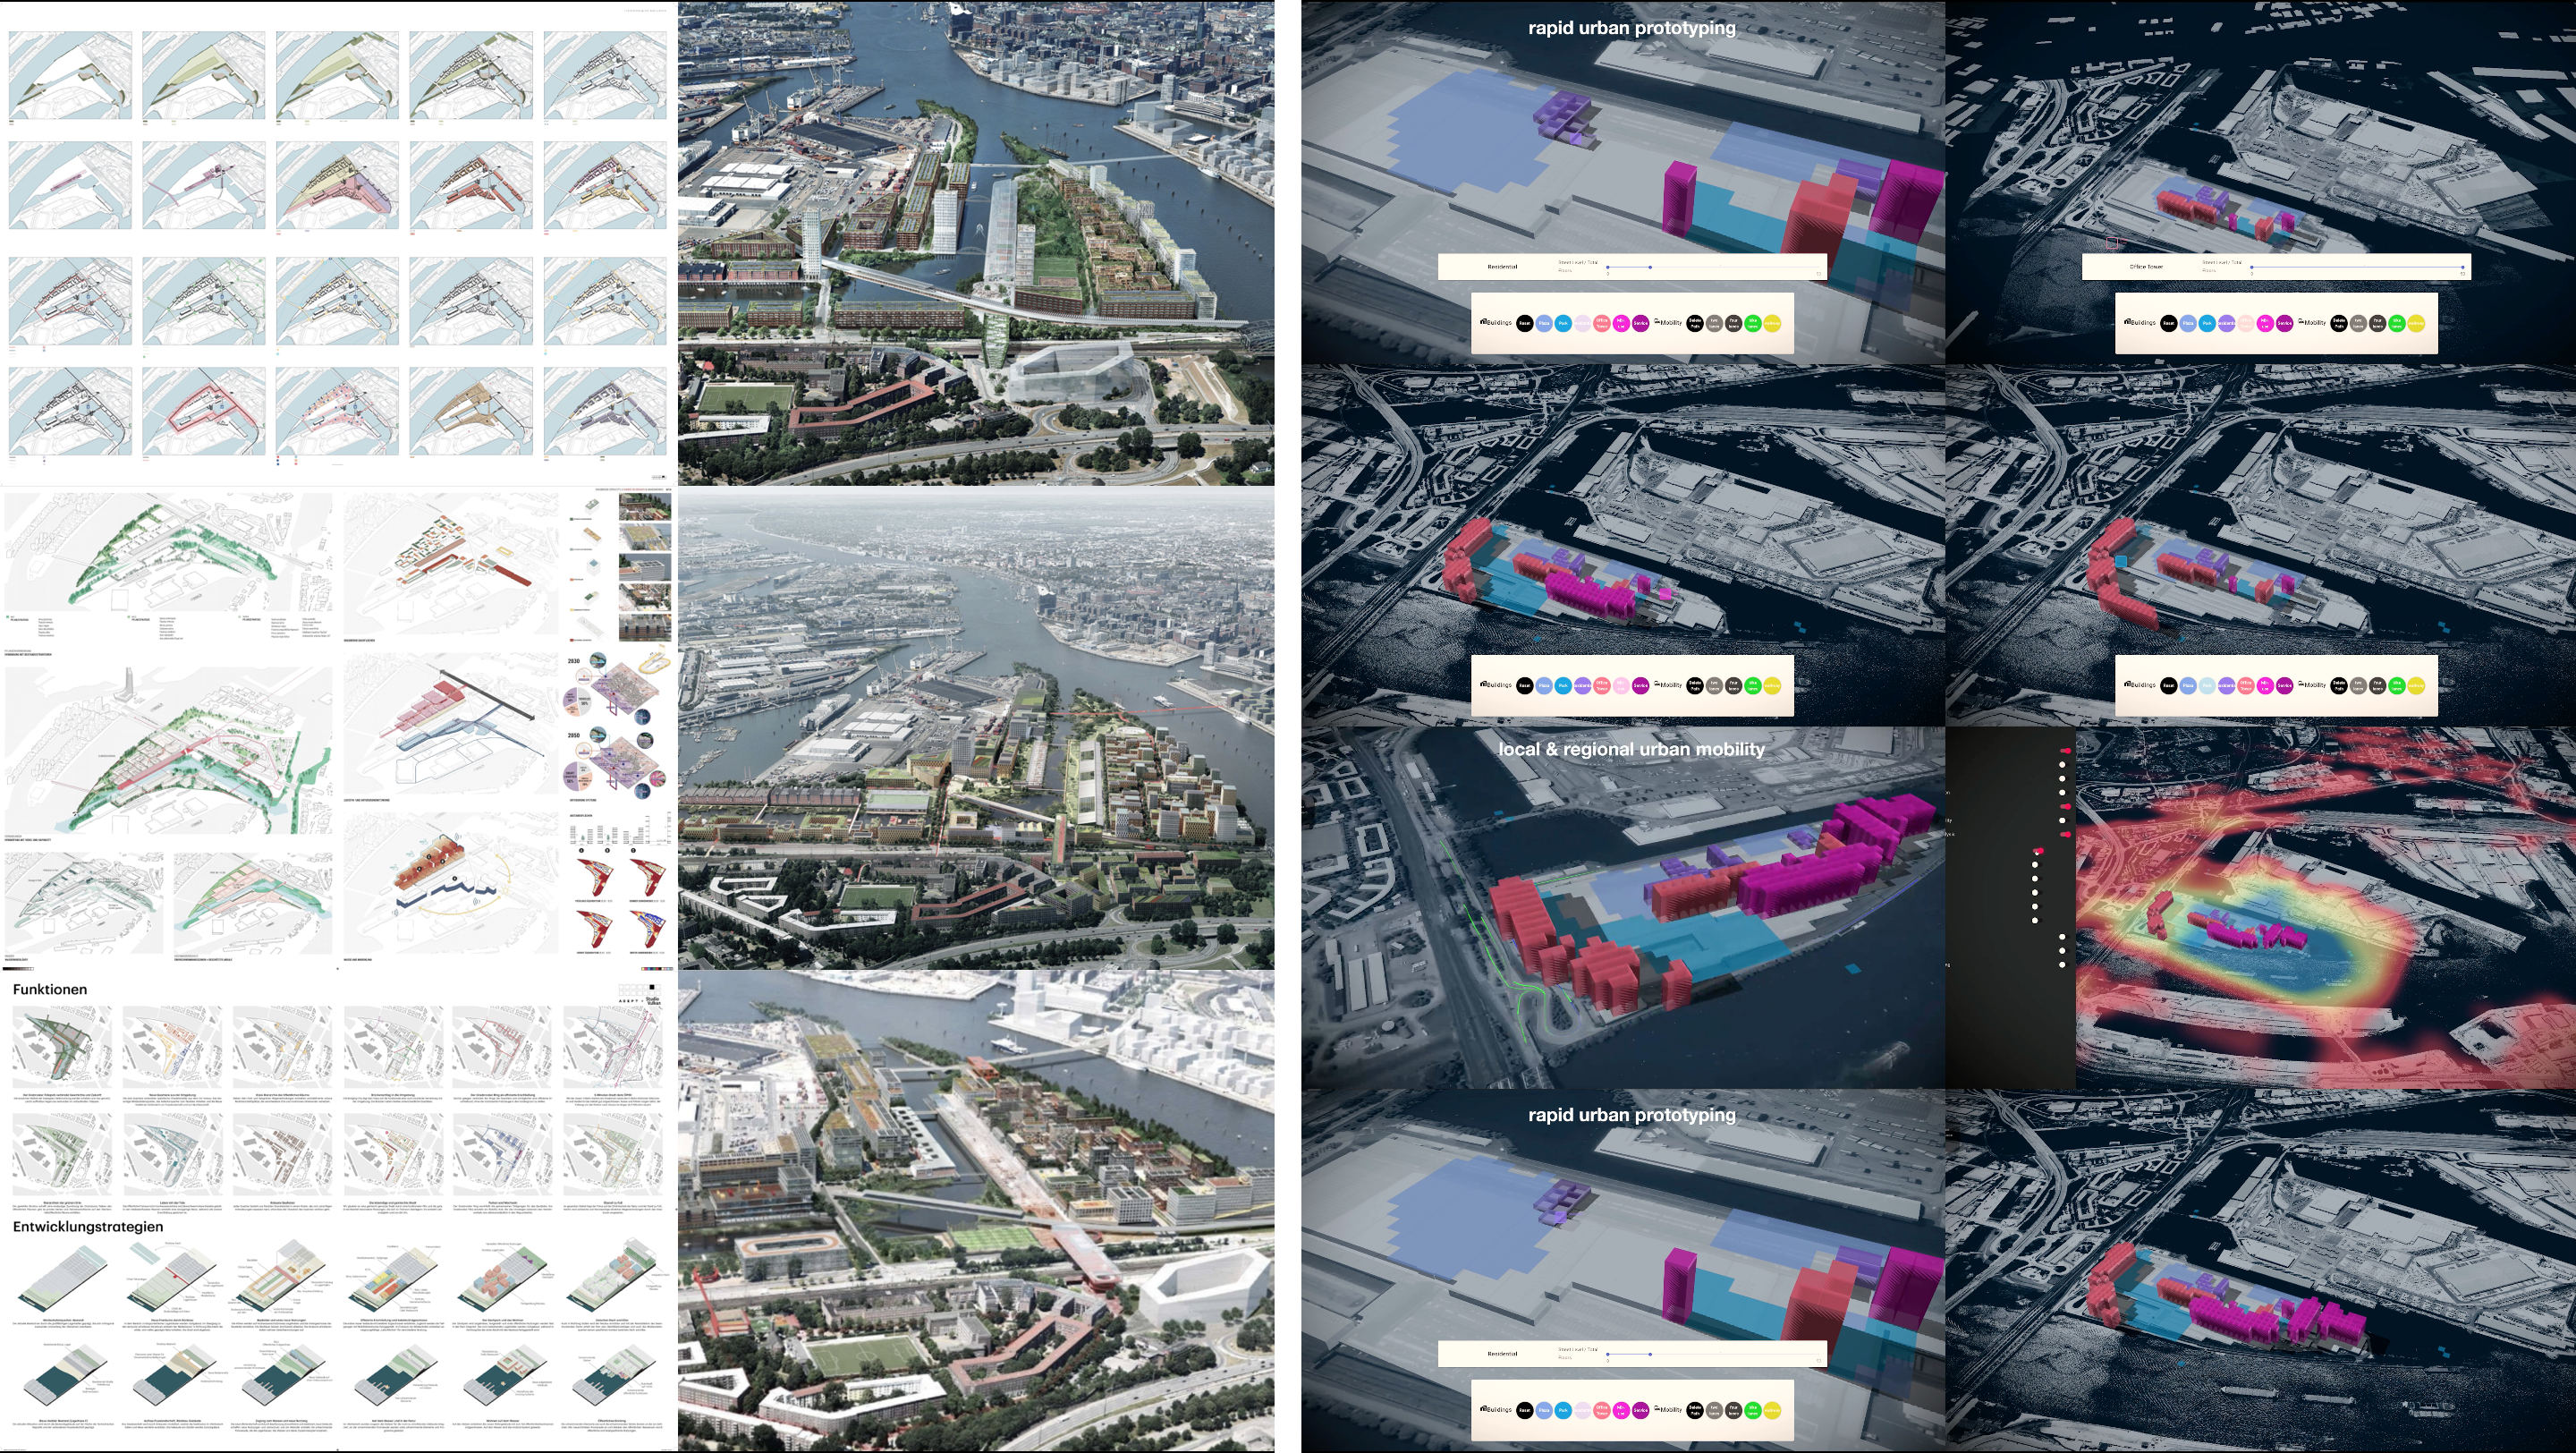
\includegraphics[width=1\textwidth]{chapters/transformation/grasbrook/figures/grsbrk5.png}
            \end{center}
            \caption{Competition submissions vs. CityScope interface. Similar to other architectural and design competitions, the Grasbrook's brief specify certain requirements for each design submission. Nevertheless, `creative freedom' and lack of a strict submission format makes it hard to properly evaluate the performance metrics of each proposal. The CityScope interface, on the other hand, is designed for an `apples-to-apples' comparisons, where the user can observe, evaluate, and correct the results of different submissions in one framework.}
            \label{fig:grasbrook_competition_vs_cs}
        \end{figure}

        \subsubsection{Motivation}
        {
            Urban development projects evolve through complex and lengthy processes: From project initiation, via public deliberation and tendering, onto the physical execution of architectural designs. In all of these stages, a multitude of stakeholders, functional requirements, and criteria must to be well coordinated \cite{alexander1990planning}. Within this process, the results of urban-design competitions play a crucial role, as their procedures and outcomes can strongly determine the shape and quality of future urban environments.
            \newline
            In this context, CityScope Grasbrook addresses two use-cases: (i) \textit{During the Design Process:} CityScope is used by design teams in the earliest phases of schematic design (SD), in which crude proposals are drafted to outline functional and spatial features of the area. In this case, the system was designed to rapidly deliver information on the effects of their drafts, to estimate their overall qualitative performance, and to optimize their spatial layout and functional programs. For example, CityScope may instantly provide answers to questions like: \textit{``How does the placement of a certain building influences the propagation of traffic noise in the area?''}
            \newline
            (ii) \textit{During Jury Review:} Here, CityScope is used later in the competition process, when expert juries assess submissions to conclude the winning entry. At this stage, CityScope helps the jurors to evaluate the submissions, to check their compliance with key criteria, and to judge the different proposals on the basis of objective performance indicators. The comparison of design proposals by way of algorithmic analysis benefits an unbiased and transparent assessment process, and can also eases the task of assessing inconsistent or non-standardized submission formats\footnote{Especially in early design phases, these deliverables could vary dramatically, from mix-media and physical models, to perspective drawings and text descriptions \cite{ben-joseph2001}.}.
        }
    }

    \begin{figure}[!htb]
        \begin{center}
            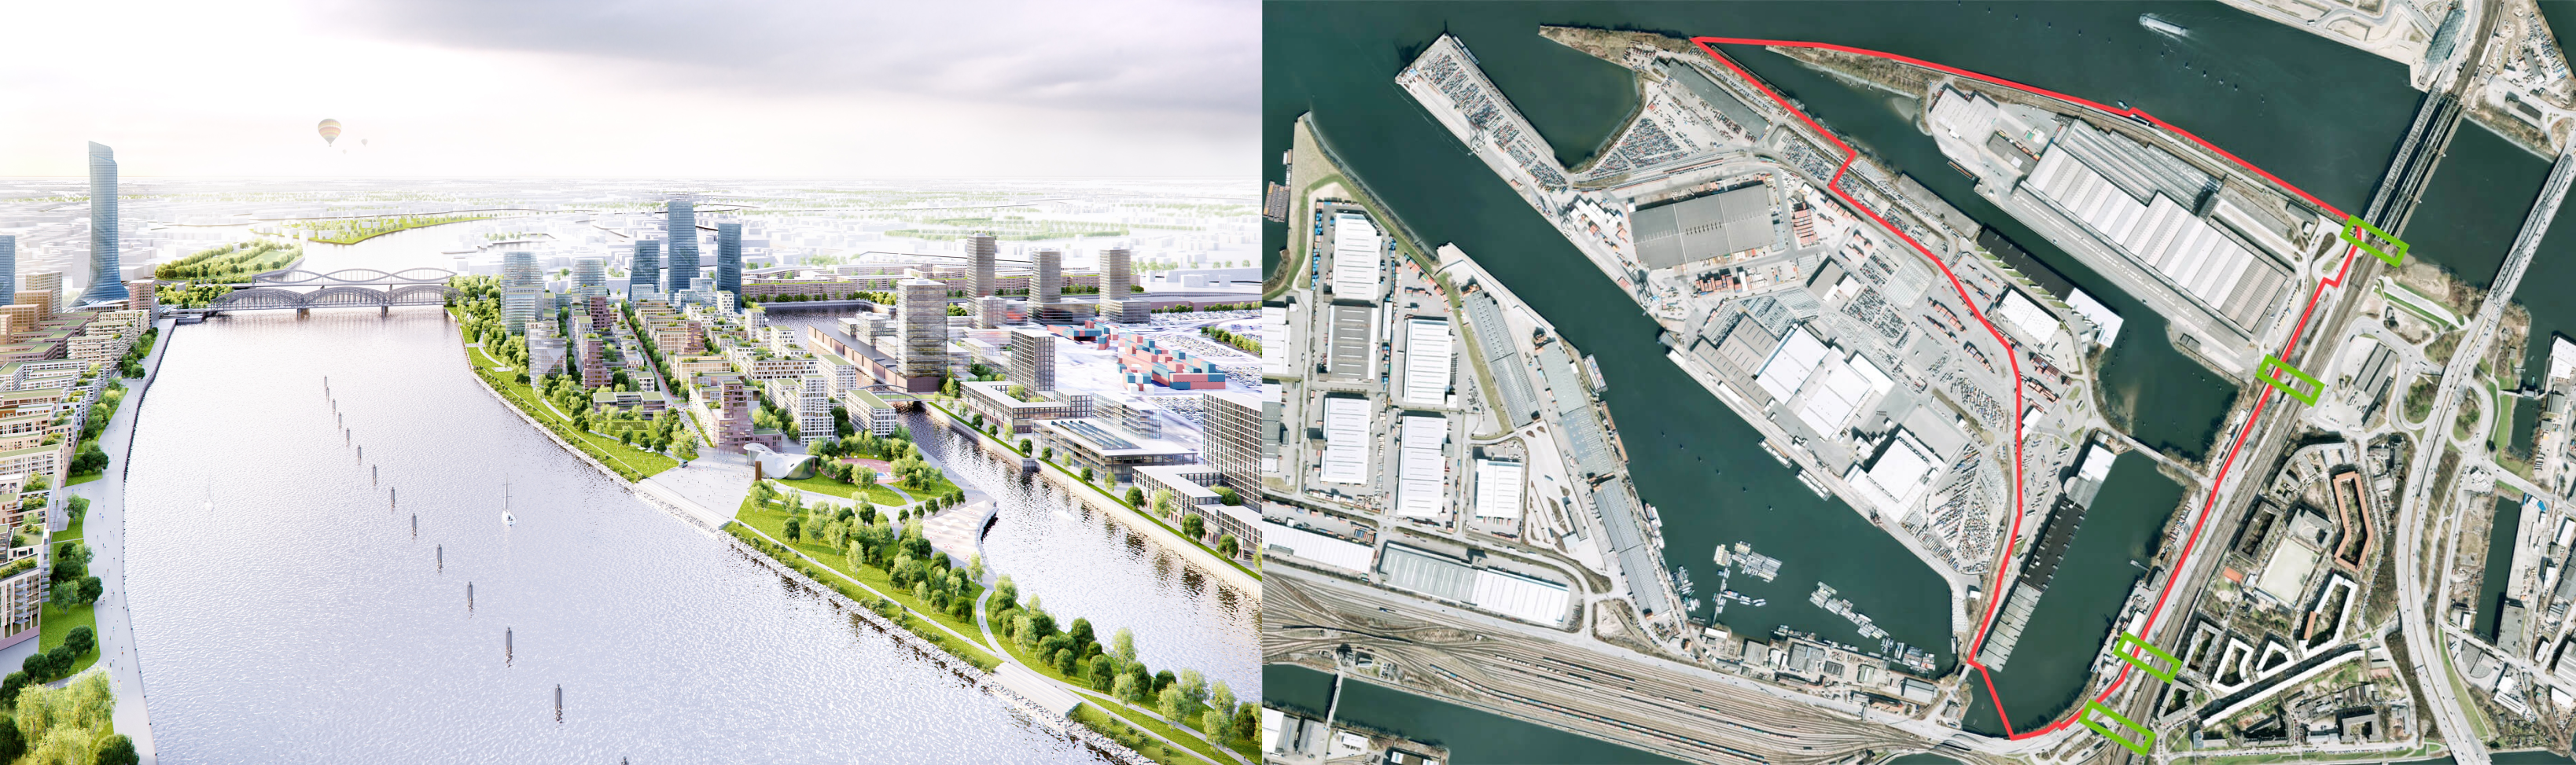
\includegraphics[width=1\textwidth]{chapters/transformation/grasbrook/figures/grsbrk1.png}
        \end{center}
        \caption{Grasbrook site (right) showing the active harbor section in the south-west, and the Veddel neighborhood to the east. (left) Previous design studies for Grasbrook, by Hosoya Schaefer Architects, Zurich.}
        \label{fig:grasbrook_site}
    \end{figure}

    \subsection{`Competitive Dialogue'}
    {
        A ``Competitive Dialogue'' is a bidding framework designed for complex urban development projects \cite{hpg15}. For the Grasbrook site, the bidding was announced EU-wide, and twelve teams (six urban-design and six landscape-design offices) were invited\footnote{The HafenCity Hamburg GmbH who published and managed the tender, acted as an intermediary between ministries, citizens, experts and design teams in order to supply data and feedback for the iterative improvement of their design schemes.}. In phase one, the teams worked independently within their professional domains; After the conceptual phase, six offices were submerged into three mixed teams, who were asked to propose an holistic landscape and urban-design solution. After the second phase, one winning team was selected by a high-level jury in April 2020.
    }



    \subsection{Platform Design}

    {
        CityScope Grasbrook utilized the unified CityScope architecture (see Section \eqref{sec:cityscope_architecture}) as a baseline for the development of a custom set of analysis modules and feedback features. This system design was well suited for the Grasbrook use-case, since it could host a myriad of analytic tools, whose interconnection enables an algorithmic analysis of complex cause-and-effect chains created by urban-design interventions.

        \begin{figure}[!htb]
            \begin{center}
                \includegraphics[width=1\textwidth]{chapters/transformation/grasbrook/figures/grsbrk3.jpg}
            \end{center}
            \caption{Grasbrook CityScope System Architecture: Following the CityScope Schema and system design, Grasbrook adapted a parallel data flow between the different components (see Section \eqref{sec:cityscope_architecture}).}
            \label{fig:grasbrook_architecture}
        \end{figure}

        \textbf{Modular Architecture:} CityScope Grasbrook was designed as an online platform first, which could later be extended to TUI and other interfaces as needed. The overall architecture consists of a frontend UI and a set of various backend analysis modules, all of which are connected via cityIO (see \eqref{subsec:csarch-cityio}). With this structure, different software applications for the analysis of specific urban KPIs (i.e. noise propagation, storm-water runoff, pedestrian accessibility) or target indicators (Gross Floor Area, FAR) can be easily plugged-in yet independently developed by different teams.
        \newline
        \textbf{Security Features:} Specific to the Grasbrook case-study, secure storage of the competitors' project data was required. Simultaneous user-access to the CityScope platform, as well as backend data management, had to comply with security and confidentiality standards. Considering legal controversies that sometimes emerge in the aftermath of design competitions, the CityScope team implemented several data security and safety measures: secure user authentications, individual usernames and passwords for each participant, access monitoring, real-time system logging and analytics. These features were implemented in the frontend UI, and the backend cityIO server.


        \begin{figure}[!htb]
            \begin{center}
                \includegraphics[width=1\textwidth]{chapters/transformation/grasbrook/figures/grsbrk4.jpg}
            \end{center}
            \caption{Translation of design submissions into CityScope grid. When complex shapes are presented, or negative volumes calculation is need for GFA calculations, the grid approach might be less accurate.}
            \label{fig:grasbrook_pixel_translation}
        \end{figure}
    }


    \textbf{Interaction Design:} As with other CityScope projects, site and intervention data is translated into the form of a grid and the CityScope Schema \eqref{sec:cityscope_architecture}, enabling faster modules' calculations and real-time user interaction. This transformation is performed by transferring the morphology of the site into a 2D raster\footnote{in the Grasbrook case, the grid was of 16x16 meters and four meters for ground level, three meters on upper levels}. Each grid cell hold information about its usage (built or unbuilt) along with its core functions (residential, commercial, educational, promenade, street, park, etc.). In the context of the Grasbrook competition, the matrix reflects (i) A standard measure for minimum street width according to heat flow and pollutant dispersion metrics \cite{yc18}; (ii) A building depth allowing natural cross-ventilation and daylight penetration \cite{mn19}; (iii) A suitable level of detail for visualization, allowing intuitive and real-time feedback for user interaction; and (iv) A documented metric for other similar cases of computational urban simulations.


    \subsection{Analytic Modules}

    {
        HafenCity Hamburg GmbH prioritized four types of analytic modules: noise propagation, storm-water runoff, walkability, and gross floor area (GFA). These modules were deemed as key in the decision-making process of the competition, as they commonly hard to infer from the design submission themselves. The following is a description of each module, and an evaluation of its performance and usability.

        \begin{figure}[!htb]
            \begin{center}
                \includegraphics[width=1\textwidth]{chapters/transformation/grasbrook/figures/grsbrk2.jpg}
            \end{center}
            \caption{Goals of each of the CityScope modules used in Grasbrook. As with other CityScope projects, each module should aim to answer a specific question. For CityScope users, the overlapping of different modules' responses creates a deeper understanding of the design tradeoffs, for example: `Would this intervention promote both easier access AND better water management?'}
            \label{fig:grasbrook_modlues_questions}
        \end{figure}


        \subsubsection{Modules Accuracy}
        {
            This project was a first opportunity to test the CityScope modular architecture in real-world use-case. This required a high level assessment of modules' quality and reliability, for both the design teams as well as the jurors. In communications to the design teams, trade-offs between usability, speed of interaction, and quality of assessment were highlighted.
            While higher accuracy and reliability could only come from expert reports and industry standard, these tend to be costly, take substantially longer time to produce, and would not be as iterative as the CityScope layouts. Since CityScope pixelates the raster of the design space, calculating the level of accuracy was done by comparing modules' output with rasterized results of analysis preformed by external committee of experts\footnote{The introduction of CityScope to the Grasbrook tender had to comply with organizational and legal constraints. Due to the academic nature of the project, it was necessary to distinguish the features and outputs of the CityScope solution from those of accredited expert tools. When introduced to the competition teams, the aim and character of the scientific experiment were communicated, and it was maintained that the solution would not deliver legally binding output or assessments, but rather provide additional support for the decision-making process.}.
        }



        \begin{figure}[!h]
            \begin{center}
                \includegraphics[width=.7\textwidth]{chapters/transformation/grasbrook/figures/grsbrk0.png}

            \end{center}
            \caption{
                Analytic modules developed for the Grasbrook competition (From the top):
                (i) CityScope noise analysis result compared to experts' analysis for the winning competition entry; (ii) CityScope results of runoff coefficients. Estimated annual runoff volumes m\textsuperscript{3} by surface type. Upper Right: Qualitative evaluation used to assess schematic map submissions; (iii) Walkability calculations results for user type `adult' and `cultural institutions'. Areas in green show the travel distance below the threshold of a five-minute walk. Upper Right: Qualitative evaluation method used to assess submission materials, including schematic maps, explanatory sketches, and pictograms.
            }
            \label{fig:grasbrook_results}
        \end{figure}

        \subsubsection{Noise Module}
        {
            Noise emission is a key concern in urban-design and city-planning. Grasbrook site is situated near major transit arteries, highways, railways, as well as an industrial port area, making the appropriate estimation of acoustic impact, a crucial item in the evaluation of design proposals \cite{e19}. In conventional planning procedures, noise performance of design proposals is usually possible only through expert evaluation in advanced stages, sometimes years after the initial competition phase has been concluded. In contrast, the noise module developed for the Grasbrook CityScope was able to model noise propagation throughout the design area in near real-time.
            \newline
            This module considers noise emitters, such as large streets and adjacent railway lines, on the basis of predicated traffic loads. It uses software developed by the French Institute of Science and Technology for Transport, Development and Networks \cite{bgppf19}, which is based on a simplified implementation of the French standard for urban noise propagation, NMPB-08 \cite{n11}. When designers interact with the CityScope grid, the noise simulation tool extracts building footprints and calculates a 2D noise distribution map. The noise emitted by simulated traffic on streets and railways is propagated through the design area, taking into account the diffractions and reflections caused by the buildings.
            \newline
            \textbf{Evaluation and Validation:} In order to evaluate the noise module accuracy, the CityScope noise module were compared to results retrieved from an established noise modeling consultancy. Figure \eqref{fig:grasbrook_results} presents the results of the analysis of the winning competition entry performed with the CityScope tool compared to the results delivered by the external consultancy. Visually, both noise maps shows similar dispersal patterns. When rasterizing both result sets, a differential map is computed to locate and visualize the differences in estimated noise levels. This differential map indicates that the total area of noise level differences greater than 10dB are below 7.5\% of the design area, whereas 53\% of the design area show deviations of max 5db. The remaining 39.5\% of the design area shows deviations between 5 and 10 dB.
            \newline
            Studies have shown that different experts evaluating noise using different national methods create results which deviate by 10 to 15dB \cite{nw05}. In this case, a main cause for the deviation results is the different calculation methods used by the CityScope and the external consultancy, which differ in the standard metrics utilized\footnote{Simplified implementation of the French NMPB-08 standard for CityScope vs. German RLS 90 standard for road noise sources and unspecified methods for propagation calculation Consultancy}. Moreover, technical differences and input assumptions influence the definition of noise modeling accuracy, such as:
            (i) Rasterized CityScope input format leads to simplifications of the design proposal, from building footprints to a grid-based input;
            (ii) Experts added higher noise levels to context-specific locations (e.g., bridges over the Elbe River);
            (iii) French and German standards use different annotation scales for noise levels;
            (iv) CityScope delivers a composite day, evening and night index (LDEN) while the method deployed by the external consultancy indexes for daytime only.
            \newline
            As a general trend, the results delivered by the CityScope generally show lower noise levels than the ones delivered by the external consultancy. Still, a proportional behavior and distribution of the noise levels underline the applicability of the tool for real-time noise modeling.
        }


        \subsubsection{Storm-water Module}
        {
            As in many other parts of the city of Hamburg, the Grasbrook district is vulnerable to flooding caused by heavy rainfall events and sea-level rise. The HafenCity Hamburg GmbH requested a storm-water module in order to evaluate the synergies between green storm-water infrastructure, comfortable microclimatic conditions, and the functional requirements for landscape design. This module calculates the surface runoff from each cell in the CityScope grid, and combines it to an annual storm-water runoff analysis. Each cell of the grid contains data about the surface type (e.g., building, street, open-space) and each type is assigned a runoff coefficient\footnote{The runoff coefficients were adapted from Table 9 of DIN 1986-100:2016-12 \cite{e16}.}. The $m^2$ area of each cell is multiplied by the runoff coefficient and by the annual rainfall $m^3/m^2*a$.
            \newline
            \textbf{Evaluation and Validation:} Today, most experts rely on schematic blueprints or renderings to evaluate storm-water potential. These schematics often lack the information necessary to evaluate the submissions beyond a baseline qualitative assessment. CityScope storm-water module uses standardized measures of surface permeability and infiltration potential, in order to estimate cumulative annual runoff volumes. While expert analysis for water-cycles usually involves a tricolor rating system, CityScope enables a quantitative comparison of the design submissions in their entirety, while still supporting qualitative assessments.
            \newline
            Nevertheless, some spatial aspects were not consistently present in all design submissions, for example: (i) Topography within the area; (ii) Directional flows within the storm-water network, and (iii) Location and size of infrastructure, such as infiltration, retention, water treatment facilities, or neighborhood cistern. Consequently, the Grasbrook version of the storm-water module did not include these aspects, either. Already in its current form, the storm-water module can deliver a valuable quantitative comparison of the designs in regards to the ratio of green and open-space, as well as annual runoff projections from differentiated surface types.
        }

        \subsubsection{Walkability Module}
        {
            Walkability is a key parameter in the evaluation of urban districts and neighborhoods design \cite{carr1969city, krier1979urban}. Human-centred urban-design promotes the development of neighborhoods that well-function without broad usage of motorized vehicles; In order to prevent unnecessary traffic and subsequent negative environmental impacts, basic amenities and socio-spatial infrastructure need to be accessible to all local residents within a minimal walking distance \cite{banerjee2011companion}. In order to identify the distribution of services and amenities during early urban-design processes, an analytic module was devised to calculate the 5-minute walkshed of a subset of amenities, such as educational, cultural or retail. The tool implements a standardized isochrone calculation using the walkable street network, a common method utilized in walkability and accessibility research \cite{dp20, dwp17}.
            \newline
            \textbf{Evaluation and Validation:} While the expert analysis was based on a qualitative evaluation of the pedestrian network, CityScope numerically calculated the accessibility based on the street network morphology in the proposal. Specifically, the module calculated accessibility to-and-from different amenity types, using three main trip profiles: adult, child, and wheelchair user. Each of the walking profiles includes an average speed and a list of surfaces through which they can traverse comfortably; For example, wheelchair users might not be able to pass through streetscape involving stairs or steep slopes. The walkability calculation for each amenity type, and each walking profile, is performed using a flood-fill calculation performed by Dijkstra's shortest path algorithm on the CityScope grids \cite{eldg14}. The CityScope walkability module enables quantitative analysis of accessibility, complementing the mostly qualitative interpretation provided by the mobility and transportation experts.
        }

        \subsubsection{GFA Module}
        {
            A common indicator for the economic and spatial feasibility of urban-design is the Gross Floor Area (GFA) \cite{fcc18}. Balancing between economic profitability (production of marketable real-estate) and spatial quality (openness, view, visibility), is a key in urban-design processes. The definition of GFA do not only affect physical parameters (e.g., distribution of light and shadow) but also local logistics and supplies, as well as the provisioning of social infrastructure (e.g., day-care or medical facilities). The CityScope GFA module calculates the aggregated GFA in square meters in respect to the classification of building-use defined in the competition brief.
            \newline
            \textbf{Evaluation and Validation:} Given the simplification imposed by CityScope grid rasterization (see Section \eqref{subsec:types_system}), the accuracy of this module depends on the granularity of the design submission, and their adherence to parallel lines, or right angles. Naturally, freeform-designs achieve lower accuracy in GFA analysis than designs based on rectangular blocks, due to deviations in the calculated floor area. In order to determine the accuracy of the module, calculations were compared with expert evaluation reports which include a cross-check of designed volumes against the definitions made by the competition brief \cite{e19}. The main land-use categories, `Commercial' and `Residential,' correspond closely with the same use types in the competition brief, whereas the CityScope category `Other' roughly translates to `Special use,' which includes cultural, educational, and sports usages.
            \newline
            Differences in type classification between CityScope and the competition brief, the transformation of the designs to the CityScope grid, and subjective data entry, contributed to misalignment in GFA module results, compared to experts evaluation. In 7 of 8 cases, the absolute difference ranged from 1\% to 27\%, with an average of absolute difference of 14\%. For one competition entry, the absolute difference was 170\% for `Other' due to the user's interpretation of non-standard mixed use types as `Other' rather than primarily `Residential' or `Commercial'. In future use-cases, a GFA module should be designed in a more flexible way, so that it could match GFA requirements of a competition brief.
        }
    }

    \subsection{Discussion}
    {
        The Grasbrook project was the first opportunity to involve CityScope system, including frontend, modules, cityIO, and other components, in a real-world design competition process.
        CityScope Grasbrook was implemented for two different use-cases: (i) Designers and planners developing design proposals during the competition, and (ii) Competition juries evaluation of these design proposals. This section evaluates the usage of CityScope for each of the two use-cases.

        \subsubsection{Strengths}
        {
            The time and cost of obtaining expert analysis is a major obstacle in the creation of feasible, sustainable and well-balanced urban-design proposals. CityScope compensates this deficit by delivering data-driven and real-time results during the design process. Moreover, CityScope architecture promotes a single data input (CityScope Grid, see Section \eqref{sec:cityscope_architecture}) which is shared across the different analytic modules. This structure avoids inputting design schemes into separated software applications, or carry out time-consuming data transfer and reformatting.
            \newline
            Additionally, CityScope provides a standardized assessment of both spatial, environmental, and social qualities of urban-design proposals. It enables an objective assessment of completely different designs, which is particularly useful when evaluating several proposals under the same set of criteria. Simplified interaction and standard visualization make the comparison of proposals substantially easier, for both the design juries and designers themselves. CityScope's standardized data format, and open-source modules provide transparency in the process of analysis and assessment, and allow technical consensus amongst domain-experts.
        }

        \subsubsection{Weaknesses}

        {
            The accuracy of the analytic modules remains a scientific and methodological challenge. Designers, juries, developers, or investors depend on clear indications and relative reliability compared to well-established methods of evaluation. While validation was preformed for the noise and rainwater modules, the discrepancy of scientific models, methodology, and data schemes, challenges an in-depth validation and refinement of other modules.
            \newline
            Even though one single data structure (CityScope Grid) can be more time efficient compared to several data inputs and separated applications, the current tool required that the designs would be manually uploaded. This was accomplished by importing multiple layers of geospatial information (e.g., existing buildings, site restrictions), as well as rasters of the first round designs, to allow users to translate them into CityScope grids. To make the input and translation process easier, users expressed interest to import data formats common for their preferred design software or competition submission files (e.g., DWG, RVT, IFC). In the future, such data conversion pipeline could be added to CityScope for automatic CAD and BIM data conversion.
        }

        \subsubsection{Opportunities}
        {
            A key benefit of CityScope is its capacity to run different types of analysis at the same time. In this respect, it has greater analytic power than evaluations which only consider one dimension at a time. By changing the layout of a plot or a building in one specific setting, impacts on many different other KPIs and metrics can be observed. By cross-connecting the various analytic modules, new inputs will simultaneously change and update other performance layers.
            \newline
            Validated CityScope modules and open-source development, can ensure that the evaluation of design proposals will not be delivered as rigid `black-box' solutions. Open-source development makes non-generic modules (such as site-specific analysis) easily adaptable to other future scenarios, and allows for better validation by the scientific community. As a digital online tool, CityScope has the potential to facilitate communication and dialogue with larger stakeholders groups, neighborhood communities, local initiatives, or academia.
        }

        \subsubsection{Threats}
        {
            The introduction of new processes and technologies can be accompanied by scepticism and rejection from its target audience. Designers tend to have well-established workflows, especially in the stressful context of design competition projects, where they rely on conceptual and technical traditions adopted over years. Similarly, jurors might not welcome the appearance of new decision-support systems: discrepancies and conflicts between expert judgement and algorithmic analysis may occur, and might be considered a disruption of established power-structures and political dominance. It is therefore critical to properly position CityScope-like tools as decision-support systems, not a replacement for experts and community discussion.
        }

    }

    \subsection{Conclusion}
    {
        CityScope Grasbrook was an initial attempt to \textit{`reinvent the competition'}, by offering an open-ended digital platform for design analysis and evaluation. This project has demonstrated its applicability for high-stake international urban-design competition, by effectively supporting the decision making of (i) Designers and planners in the process of developing sustainable urban-designs proposals, and (ii) Competition juries mandated for the evaluation of the final proposals. To both, CityScope provided instant assessment and analytic evidence via multiple key metrics.
    }
}























    %%%%%%%%%%%%%%%%%%%%%%%%%%%%%%%%%%%%%%%%%%%%%%%%%%

    \section{Discussion: UHCI for Urban Transformation}
     {
      This chapter explored the core design principles of the CityScope platform, and the ways it supports several urban transformation processes in real-world planning context. It reviewed the CityScope ecosystem, with an emphasis on the interoperability of data and analysis using the CityScope Schema, cityIO, backend modules, and frontend interfaces.
      Most use-cases in this chapter demonstrated the way CityScope supports the analysis of rather traditional urban indicators, such as accessibility, energy, urban-from, or vehicular mobility. Yet beyond these metrics, CityScope aims to asses and predict more subtle urban indicators, such as human interaction and social dynamics. The next chapter, \textit{Prediction} \eqref{ch:prediction}, looks into CityScope models and modules used to provide predictive analysis on more implicit matrices. It focuses on questions of movement, social dynamics, as well as the appearance of the city, as proxies to the evaluation of changes in the built environment.
     }

}
%%%%%%%%%%%%%%%%%%%%%%%%%%%%%%%%%%
\chapter{Prediction}\label{ch:prediction}

{
    \section{Introduction}
     {
      The ability to predict the impact of transformation on urban environments is a critical aspect of city-planning. Unlike other industries, urban interventions cannot sustain trial-and-error or A-B testing, thus requiring high degree of confidence and well established risk-aversion mechanisms \cite{doi:10.1080/14649357.2015.1127994, banerjee2011companion}. Urban forecasting could be generally described via a two axes graph: (i) the prediction time-frame, and (ii) the social - physical spectrum (see Figure \eqref{fig:predictions_axis})
      .\newline
      For example, predicting the shadows casted by a new building, is directly correlated to the building's context, as well as to its bulk and shape. Evidently, as long as the earth spins around the sun, the results of shadow modeling should be consistent, and the model describing this phenomena could be reused indefinitely.
      On the other end, a predictive model of potential human interaction in a public plaza, would share much less consistency across time and space. This model would heavily rely on social and cultural aspects, as well as physical attributes of the urban realm, such as the plaza's shape, or its proximity to certain amenities. This class of predictions, which focuses on spatial, temporal, and social aspects, is clearly harder to construct, validate, and reuse, but can make significant impact on decision-making. As reviewed in Section \eqref{subsec:andorra-data-observatory-mobility}, this class of predictions is slowly becoming mainstream in urban processes, with the growing access to location, activity, and behavioral data, as well as new computation and modeling techniques \cite{jiang2017activity, Calabrese2014, Batty2013, moro2021mobility}.
     }

    \begin{figure}[!htb]
        \begin{center}
            \includegraphics[width=0.8\textwidth]{chapters/prediction/figures/predictions_chart.png}
        \end{center}
        \caption{The landscape of urban predictions. This is a visual clustering of the high-dimensionality of different urban models. The horizontal axis represents the degree of `concreteness' for each prediction (i.e., where does this metric seats between the less tangible and more physical?). The vertical axis depicts the longevity of the prediction (i.e., how far into the future can this metric be predicted?). The size of the dots hints to the estimated span of the prediction across the two axes; For example, predicting shadows is more concrete and longer-term than predicting human behavioral patterns.}
        \label{fig:predictions_axis}
    \end{figure}

    \section{CityScope Prediction: Case Studies}
     {
      The previous chapter discussed ways by which CityScope supports predictions of long-term, physical aspects of the built environment. These included assessments ranging from Gross Floor Area, storm-water runoff, and building energy, to more complex models, such as noise propagation (see \eqref{ch:transformation}).
      \newline
      This chapter focuses on a class of predictive models at the intersection of human behavior and the built environment. These projects combine geo-spatial attributes (such as urban form, POIs, and street network graphs), socio-behavioral properties (interpreted from high-resolution telecom data), and other discrete datasets.
      In the \textit{CityScope MoCho} project (see Section \eqref{sec:modeChoices}), mobility mode choices were simulated using a city-wide synthetic population. Static data, such as census and National Household Travel Surveys (NHTS) were used to construct simulated profiles of daily commuters and assign them to home-work and 3rd places anchors. By interpreting plausible trips from socio-demographic data, the model forecasts how small scale changes to land-use can affect large scale mobility behaviors.
      \newline
      A simulated urban population can also help to understand emergence and agglomeration patterns. In CityScope \textit{Volpe}, \textit{Andorra} and \textit{Champs-Élysées} (see \eqref{sec:and_abm}, \eqref{sec:cityscope_volpe}, \cite{ChampsEl64:online}) Agent Based Models are used to simulate trips, `collision potential', and mode-choice changes caused by urban-design transformations. A similar approach was taken in the \textit{Hamburg Port-City Model} \cite{lopez2019testing}, in which an ABM was built to predicate changes to tourist activity in transit hubs and the city's port, given minor adjustments to queuing and boarding. A different type of predictions involves the usage of data-driven models to forecast implicit and `subtle' changes in urban environments. The \textit{DeepScope} \eqref{sec:deepscope} project uses Generative Adversarial Networks (GAN) to `imagine' streetscapes of future urban developments\footnote{Upcoming work in this domain will correlate behavioral patterns and user-experiences of urban streets, with the visual aspects of new urban development.}.
      \newline
      The rest of this chapter will describe how these implicit models were implemented in several CityScope projects.
     }

    %%%%%%%%%%%%%%%%%%%%%%%%%%%%%%%%%%%%%%%%%%% 
    \section{MoCho}\label{sec:cityscope-mocho}
{
    \subsection{Introduction}
    {
        Understanding the impact of city-planning on mobility habits of urban dwellers is fundamental to well functioning cities. Nevertheless, it is challenging to predict, communicate, and demonstrate the correlation between minor urban interventions and metropolitan scale mobility mode-choices (MC). CityScope `MoCho' is a real-time MC modeling and prediction module that simulates MC of individuals in a metro region, in response to small-scale urban-design transformation. The prediction models consider individual characteristics and attributes of available alternatives, and are calibrated using survey data. To explore MoCho MC predictions, users interact with the CityScope TUI which triggers new MC predictions, alongside their impacts based on land-use, density or spatial proximity. As a case-study, MoCho has been developed to simulate MC for the Boston metro area, focusing on a 14 acres development site in Kendall Sq. (see Section \eqref{appendix:playground}). The choice model was fitted and the parameters showed significant associations with a range of explanatory variables, including travel times, residential and employment densities, as well as personal attributes like age, gender, education-level and home-ownership.
    }



    \begin{figure}[!htb]
        \centering
        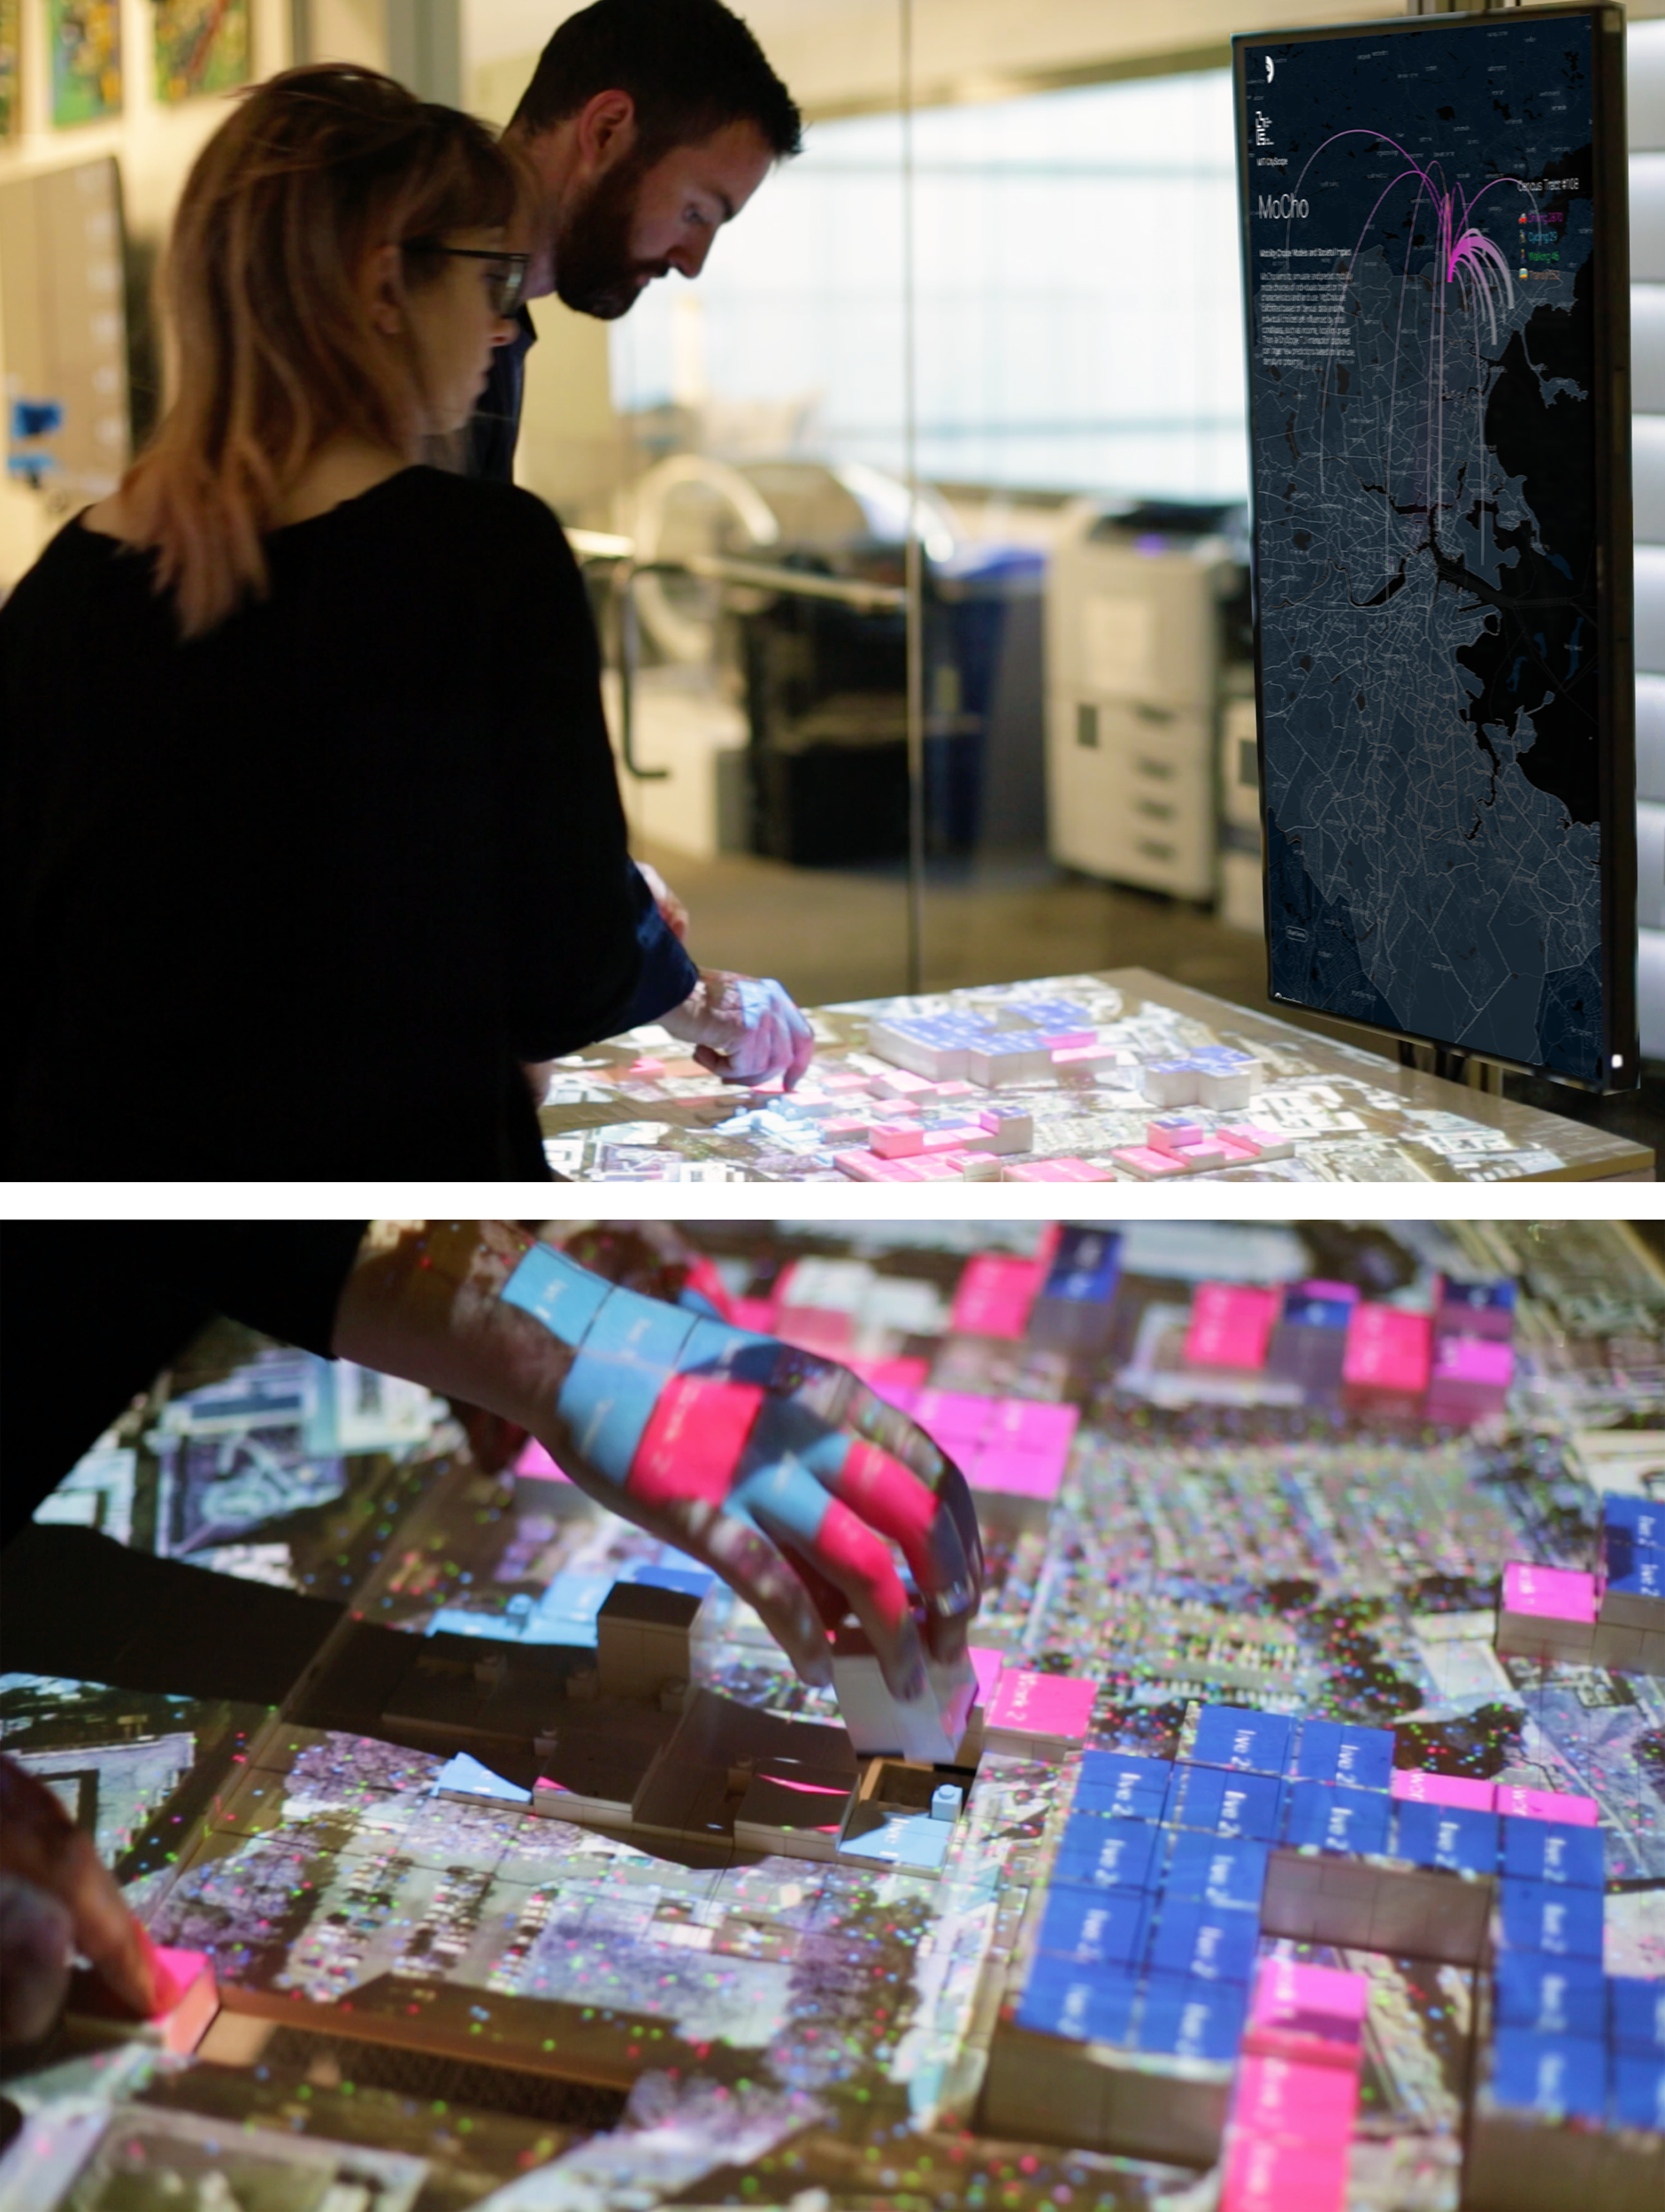
\includegraphics[width=.7\linewidth]{chapters/prediction/mocho/figures/mocho2.png}
        \caption{
            MoCho and CityScope TUI. Interaction results are computed and visualized on both vertical (metro-scale) and horizontal (parcel-scale) planes. A TUI slider (bottom left corner) allows density and building-height iteration for the land-use type used as the slider handle.
        }
        \label{fig:mocho_tui}
    \end{figure}

    \subsection{Motivation}
    {
        The individual choices urban dwellers make about their mobility and transportation behavior have profound impacts on their own lives, as well as on society as a whole. Motorized transportation leads to negative external impacts such as carbon emissions and air pollution, whereas active mode-choices such as walking and cycling improve the physical and mental health of travelers \cite{doorley2015quantifying, mueller2015health}. Urban-planning can influence these mobility choices and their societal impacts by organizing spatial land-uses and infrastructure to encourage short trips using active modes \cite{handy2002built, saelens2003environmental}. Statistical learning methods have been used successfully both in research and in practice to predict the mode-choices of travellers in response to urban interventions \cite{ben1999discrete, wardman2007factors, habib2009investigation, buehler2016bikeway}.
        \newline
        Making predictions through statistical models, generally involves the combination of various computing platforms\footnote{Most commonly in R \cite{hasan2014fast}, Stata \cite{gu2013fitting}, specialized transportation modeling software such as SimMobility \cite{adnan2016simmobility} or Python and GIS plugins.}. These may carry steep learning curves, require specialized skills, and feature limited capabilities for real-time interaction \cite{ben-joseph2001}. In this study, a CityScope instance was devised to overcome these challenges using a combination of real-time statistical models with an interactive, real-time user interface.
    }

    \subsection{Data and Modeling} \label{sec:mocho-models-data}

    {
        MoCho makes use of publicly available datasets which cover major urban areas in the US; This ensures that the methodology presented here can be replicated for the vast majority of American cities. The main data resources used are specified in Table \ref{tab:mocho-dataSources}.

        \begin{table*}[!tb]
            \centering
            \begin{adjustbox}{width=\textwidth}
                \begin{tabular}{ll}
                    \hline
                    \textbf{Resource}                              & \textbf{Description}                                                               \\
                    \hline
                    Public Use Microdata Sample (PUMS)             & Individual person and household level survey data for the USA                      \\
                    American Community Survey (ACS)                & Aggregated demographic data for administrative zones in the USA                    \\
                    OpenStreetMap (OSM)                            & An open-source editable map of the world \cite{haklay2008openstreetmap}            \\
                    Open Source Routing Machine (OSRM)             & An API which provides routing information using OSM data \cite{huber2016calculate} \\
                    Open Trip Planner (OTP)                        & A server which computes multi-modal transport itineraries \cite{OTP}               \\
                    Census Transportation Planning Products (CTPP) & A special tabulation of the ACS data for commuting characteristics                 \\
                    \hline
                \end{tabular}
            \end{adjustbox}
            \caption{Data resources used for US cities in CityScope MoCho}
            \label{tab:mocho-dataSources}
        \end{table*}

        These data sources are used to generate a synthetic population and to calibrate a model which could predict their mobility behaviors in response to changes, such as new residential or commercial development. The modeling can be described in four steps: (i) Population synthesis; (ii) Home and job location choices; (iii) Transportation mode-choice; and (iv) Impact assessment. Each of these steps is outlined below.
    }

    \subsubsection{Population Synthesis}
    {
        Mobility behaviors can be analyzed using two main approaches: (i) An aggregate approach, which divides the area into zones and predicts aggregates inter-zonal flows, or (ii) A disaggregate approach, which recognizes that urban mobility patterns are the result of many decisions made by individuals. The disaggregate approaches directly explain why an individual makes a choice given their circumstances, and therefore they are better able to predict how those choices may change in different circumstances \cite{koppelman2006self}. Due to privacy and data availability constraints, it is generally not practical to make predictions with respect to real population. Instead, it is common practice to use population synthesis techniques in order to produce a \textit{Synthetic Population}, and to make predictions with respect to these individuals. The methods take individual household-level demographic profiles and zonal aggregate demographic data, and allocate the individual records to zones in order to create the synthetic population. Some common techniques include Iterative Proportional Fitting \cite{beckman1996creating, guo2007population}, convex optimization \cite{vovsha2015new}, and Bayesian methods \cite{sun2015bayesian}.
        \newline
        The PUMS survey data used here includes the home Public Use Microdata Area (PUMA) and place-of-work PUMA for each respondent, where each PUMA corresponds to a set of census tracts. In order to model commuting trips at a tract-to-tract level, the population synthesis process needs to allocate each individual to a home and work census tract pair. A simple Bayesian method is utilized for this purpose, using the origin-destination flows from the CTPP data as well as aggregate demographic data from the ACS. PUMS individuals with attributes $A$, home PUMA $H$ and work PUMA $POW$ are assigned to an origin-destination (O-D) pair $w_{ij}$ according to the probability calculated with equation \eqref{mocho-eq-bayes}.

        \begin{equation}\label{mocho-eq-bayes}
            P(w_{ij}|A)\propto\delta_{ij}\prod_{a \in A}P(a|w_{ij})P(w_{ij})
            \\
            \quad where
            \\
            \quad
            \delta_{ij}=
            \begin{cases}
                1, & \text{if}\ H\subset i \text{ and } POW\subset j \\
                0, & \text{otherwise}
            \end{cases}
        \end{equation}

        The prior probabilities $P(a|w\_{ij})$ and $P(w\_{ij})$ may be obtained from the ACS aggregate demographic data and the CTPP O-D data.
    }

    \subsubsection{Home and Employment Location Choices}
    {
        MoCho aims to simulate the changes in home and work locations in response to amended land-use, density and spatial organization. It was assumed that when a residential or employment unit appears in a census tract, new residents or workers also appear. The number of new people is determined by the density of the unit; some demographic attributes, such as income or job sector, may be determined by the unit type. It is also assumed that the conditional probability distribution of the new residents' demographic attributes and work locations, is similar to that of the existing residents of that same tract, conditional on the known attributes. Therefore, the new resident can be simulated by cloning a randomly sampled person with the same home location tract and attributes from the synthetic population. A similar process is used to assign home locations to new workers; This location choice can be expected to be accurate for small changes to the land-uses and densities in a district but for more substantial changes, a more sophisticated model may be required.
    }

    \subsubsection{Mode-Choices}\label{sec:modeChoices}

    {
        The choice of transportation mode for each synthetic individual's commute should be predicted in response to each intervention. The mode-choices (MC) are modelled using a logit-based discrete choice model\footnote{Discrete choice models has been used extensively by researchers and practitioners in modeling of decisions including home location, work location and mode of transportation. An advantage of discrete choice models over other classification models is that their estimated parameters have economic interpretations; This means that the final model results can be easily understood by practitioners \cite{train2009discrete}.}. Discrete choice models assume that individual decision-makers select the alternative which maximizes their utility from their available options.
        \newline
        The utility is composed of a systematic component and a stochastic component: The systematic portion of the utility is (i) an additive function of attributes of the decision maker, (ii) attributes of the alternative, and (iii) interactions between both. This stochastic component is needed because in reality, two people with the same measured attributes may take different decisions when faced with similar alternatives. This component is typically assumed to be Gumbel distributed due to computational advantages and this leads to the logit formulation. These models can be defined by the following expressions \cite{koppelman2006self}:

        \begin{equation}\label{dcm}
            %   \begin{aligned}
            U(X_i, S_t)\geq U(X_j, S_t) \forall j \in C
            \quad \text{and}\quad
            U_{it}=V_{it} + \epsilon_{it}
            \quad \text{and}\quad
            V_{it}=V(S_t)+V(X_i)+V(S_t,X_i)
            %   \end{aligned}
        \end{equation}

        where $C$ is the choice set, $i$ is the alternative chosen by decision maker $t$,  $U_{it}$ is the true utility of alternative $i$ to decision maker $t$, $X_i$ are the attributes of option $i$, $S_t$ are the attributes of person t, $V$ is the systematic utility and $\epsilon$ is the stochastic utility.
        \newline
        The parameters of the logit model must be calibrated with individual-level stated-choice or revealed-choice data. For MoCho, individual observations from the PUMS data could be used for this calibration. The PUMS survey data contains 12 different options for MC but for the purpose of this work, this list is simplified to 4 major modes: car, bicycle, walk and public transportation modes. The explanatory variables considered for inclusion in the model include person attributes from the PUMS data (such as: age, income, gender, education level and employment type), attributes of the home and workplace census tracts from the ACS data, and the estimated travel times and costs for each mode and each trip. The travel times for each census tract pair were estimated by querying the OpenStreetMap API (for walking, cycling and driving times) and Open Trip Planner (for public transit travel times) \cite{OTP}. The PUMS data and ACS data contain hundreds of variables and so some exploratory analysis and feature engineering needs to be done to create a list of candidate features prior to model fitting. Once the features have been selected, the coefficients of each features can be estimated by maximum likelihood estimation, in this case using the python library `pylogit'.
    }


    \begin{figure}[!htb]
        \centering
        \includegraphics[width=.75\linewidth]{chapters/prediction/mocho/figures/mocho0.png}
        \caption{Software architecture. The CityScope table data is sent to cityIO from the tangible interface made with LEGO. cityIO stores that data to have it available to the MoCho computation module. MoCho combines this data with other geo-data from the Geo server and performs computation. The Frontend visualizes the table state and mode-choices. Each arrow indicates an HTTP response.}
        \label{fig:mocho_arch}
    \end{figure}


    \subsection{System Architecture}

    {
        CityScope MoCho is designed to allow decision-makers, planners and community members to experiment with different land-uses and spatial organizations, and understand their impact on mobility choices. As described in Section \eqref{sec:cityscope_architecture}, MoCho included cityIO, CityScope Schema, and and an early version of the CSjs frontend. It practiced the principal concept of separating frontend, backend, and microservices, and it was allowing the parallel development and maintenance of each component independently. Nevertheless, MoCho was still lacking the flexibility of later CityScope architecture, such as in the previously discussed Grasbrook project (see Section \eqref{sec:grasbrook}).
        \newline
        In this case study, the system setup consists of a CityScope TUI, including a tabletop 3D urban model, a projection scheme, and other feedback devices. The software, illustrated in Figure \eqref{fig:mocho_arch}
        consists of four parts: (i) TUI and frontend; (ii) Data management; (iii) Backend computation for the MC model; and (iv) A spatial Geo-Server. The rest of the section describes each of the system's different components, the data-flow and networking between them.




        \subsubsection{User Interaction}
        {
            MoCho uses CityScoPy \eqref{subsec:csarch-cityscopy} to recognize monochromatic tags over a uniform grid. Added to this project were TUI sliders constrained on one axis and scanned along an indentation. Unlike other tiles, slider emits a float value ($0 - 1$) that is added to the rest of the grid data and transmitted to cityIO server \eqref{subsec:csarch-cityio}. A feedback module contains display screens and projectors communicate the analysis outcomes back to the user.
        }
        \subsubsection{cityIO}
        {
            MoCho used an early version of the CityScope microservices architecture. The MoCho API (described in Section \eqref{sec:mocho_api}) listens to cityIO to attain the TUI state, and combines it with data from the Geo-Server to make MC predictions. The flow of data within this system has four steps: (i) The TUI interface reads the tags and sends them via HTTP request to cityIO; (ii) cityIO receives the CityScope data and exposes it to MoCho API; (iii) In combination with the data from the Geo-Server, MoCho predicts and exposes the result by it's own HTTP endpoint; (iv) The CSjs frontend collects data from the different APIs and visualizes the overall result on the CityScope instance.
        }
        \subsubsection{MoCho API}\label{sec:mocho_api}
        {
            The MoCho API is the module responsible for predicting the mobility choices of each simulated individual, in response to changes to the state of the TUI data. When a change is detected, the module creates new synthetic population corresponding to the amended residential or commercial buildings, and assigns their home and work locations as described in Section \eqref{sec:mocho-models-data}. The residential and employment densities of the tracts containing the new buildings are also updated. The modes of transportation for each commuting trip are then predicted using the MC model. The results are sent as JSON format and are exposed to the CSjs frontend for visualization.
            \newline
            User interactions can lead to changes in the mobility choice and impact predictions in three ways: First, when residential and commercial units are added to denser, more central parts of the city, the newly spawned individuals will be more likely to choose workplaces with shorter commutes. Second, when new units are added to parts of the city where the current population of residents/workers has personal characteristics which tend to favor alternative mode (cycling for example), the newly spawned people will tend to inherit those characteristics. Lastly, the addition of new buildings affects the attributes of the census tract, such as overall residential and employment density and these attributes can affect the mode-choice probabilities of all people living and working in the census tract.
        }

        \subsubsection{Geodata API}
        {
            Census tracts and other geo-spatial data are required to compute MC as well as to visualized the prediction. For this purpose, an additional module was designed to service \verb|GEOJSON| data for the study area. In the case study of Section \eqref{subsec:mocho-volpe}, geo-data for the Boston Metro area and for a selected interactive region in Cambridge, MA were served. This API can be easily scaled to serve MoCho or other modules in different regions, given access and availability of spatial data.
        }
    }

    \subsection{Case Study: Volpe}\label{subsec:mocho-volpe}
    {
        To examine the MC model in a real-world mobility environment, a site under development in Kendall Sq., Cambridge MA was selected. A CityScope TUI, a cityIO endpoint, and GeoServer instance were built for this site. This Section will explore the MoCho Volpe instance in details.

        \subsubsection{CityScope MoCho}
        {
            The setup shown in Figure \eqref{fig:mocho_components} was designed for the Volpe site and its immediate surroundings\footnote{Covering a region of $\sim$0.5sqkm at the scale of 1:500, where each 4x4 LEGO-tile represents a 16sqm or 4sqm per each LEGO stud.}. For interaction, six major classes of land-use were defined: open and green spaces, streets, high-income housing ($Housing-1$), mid-to-low income housing ($Housing-2$), large companies' development ($Commercial-1$), and startup and co-working spaces development ($Commercial-2$). Each LEGO tile on the CityScope TUI is classified with one of these land-uses.
            Allocating different tiles next to the each other (e.g., two tiles of type $housing-2$ and one tile of type $commercial-1$) would be translated as a mixed-use structure with multistory housing and offices. The TUI slider adds an additional dynamic control which allows the density (height) of all cells of the same class to be altered concurrently, as shown in Figure \eqref{fig:mocho_components}.
        }

        \begin{figure}[!htb]
            \centering
            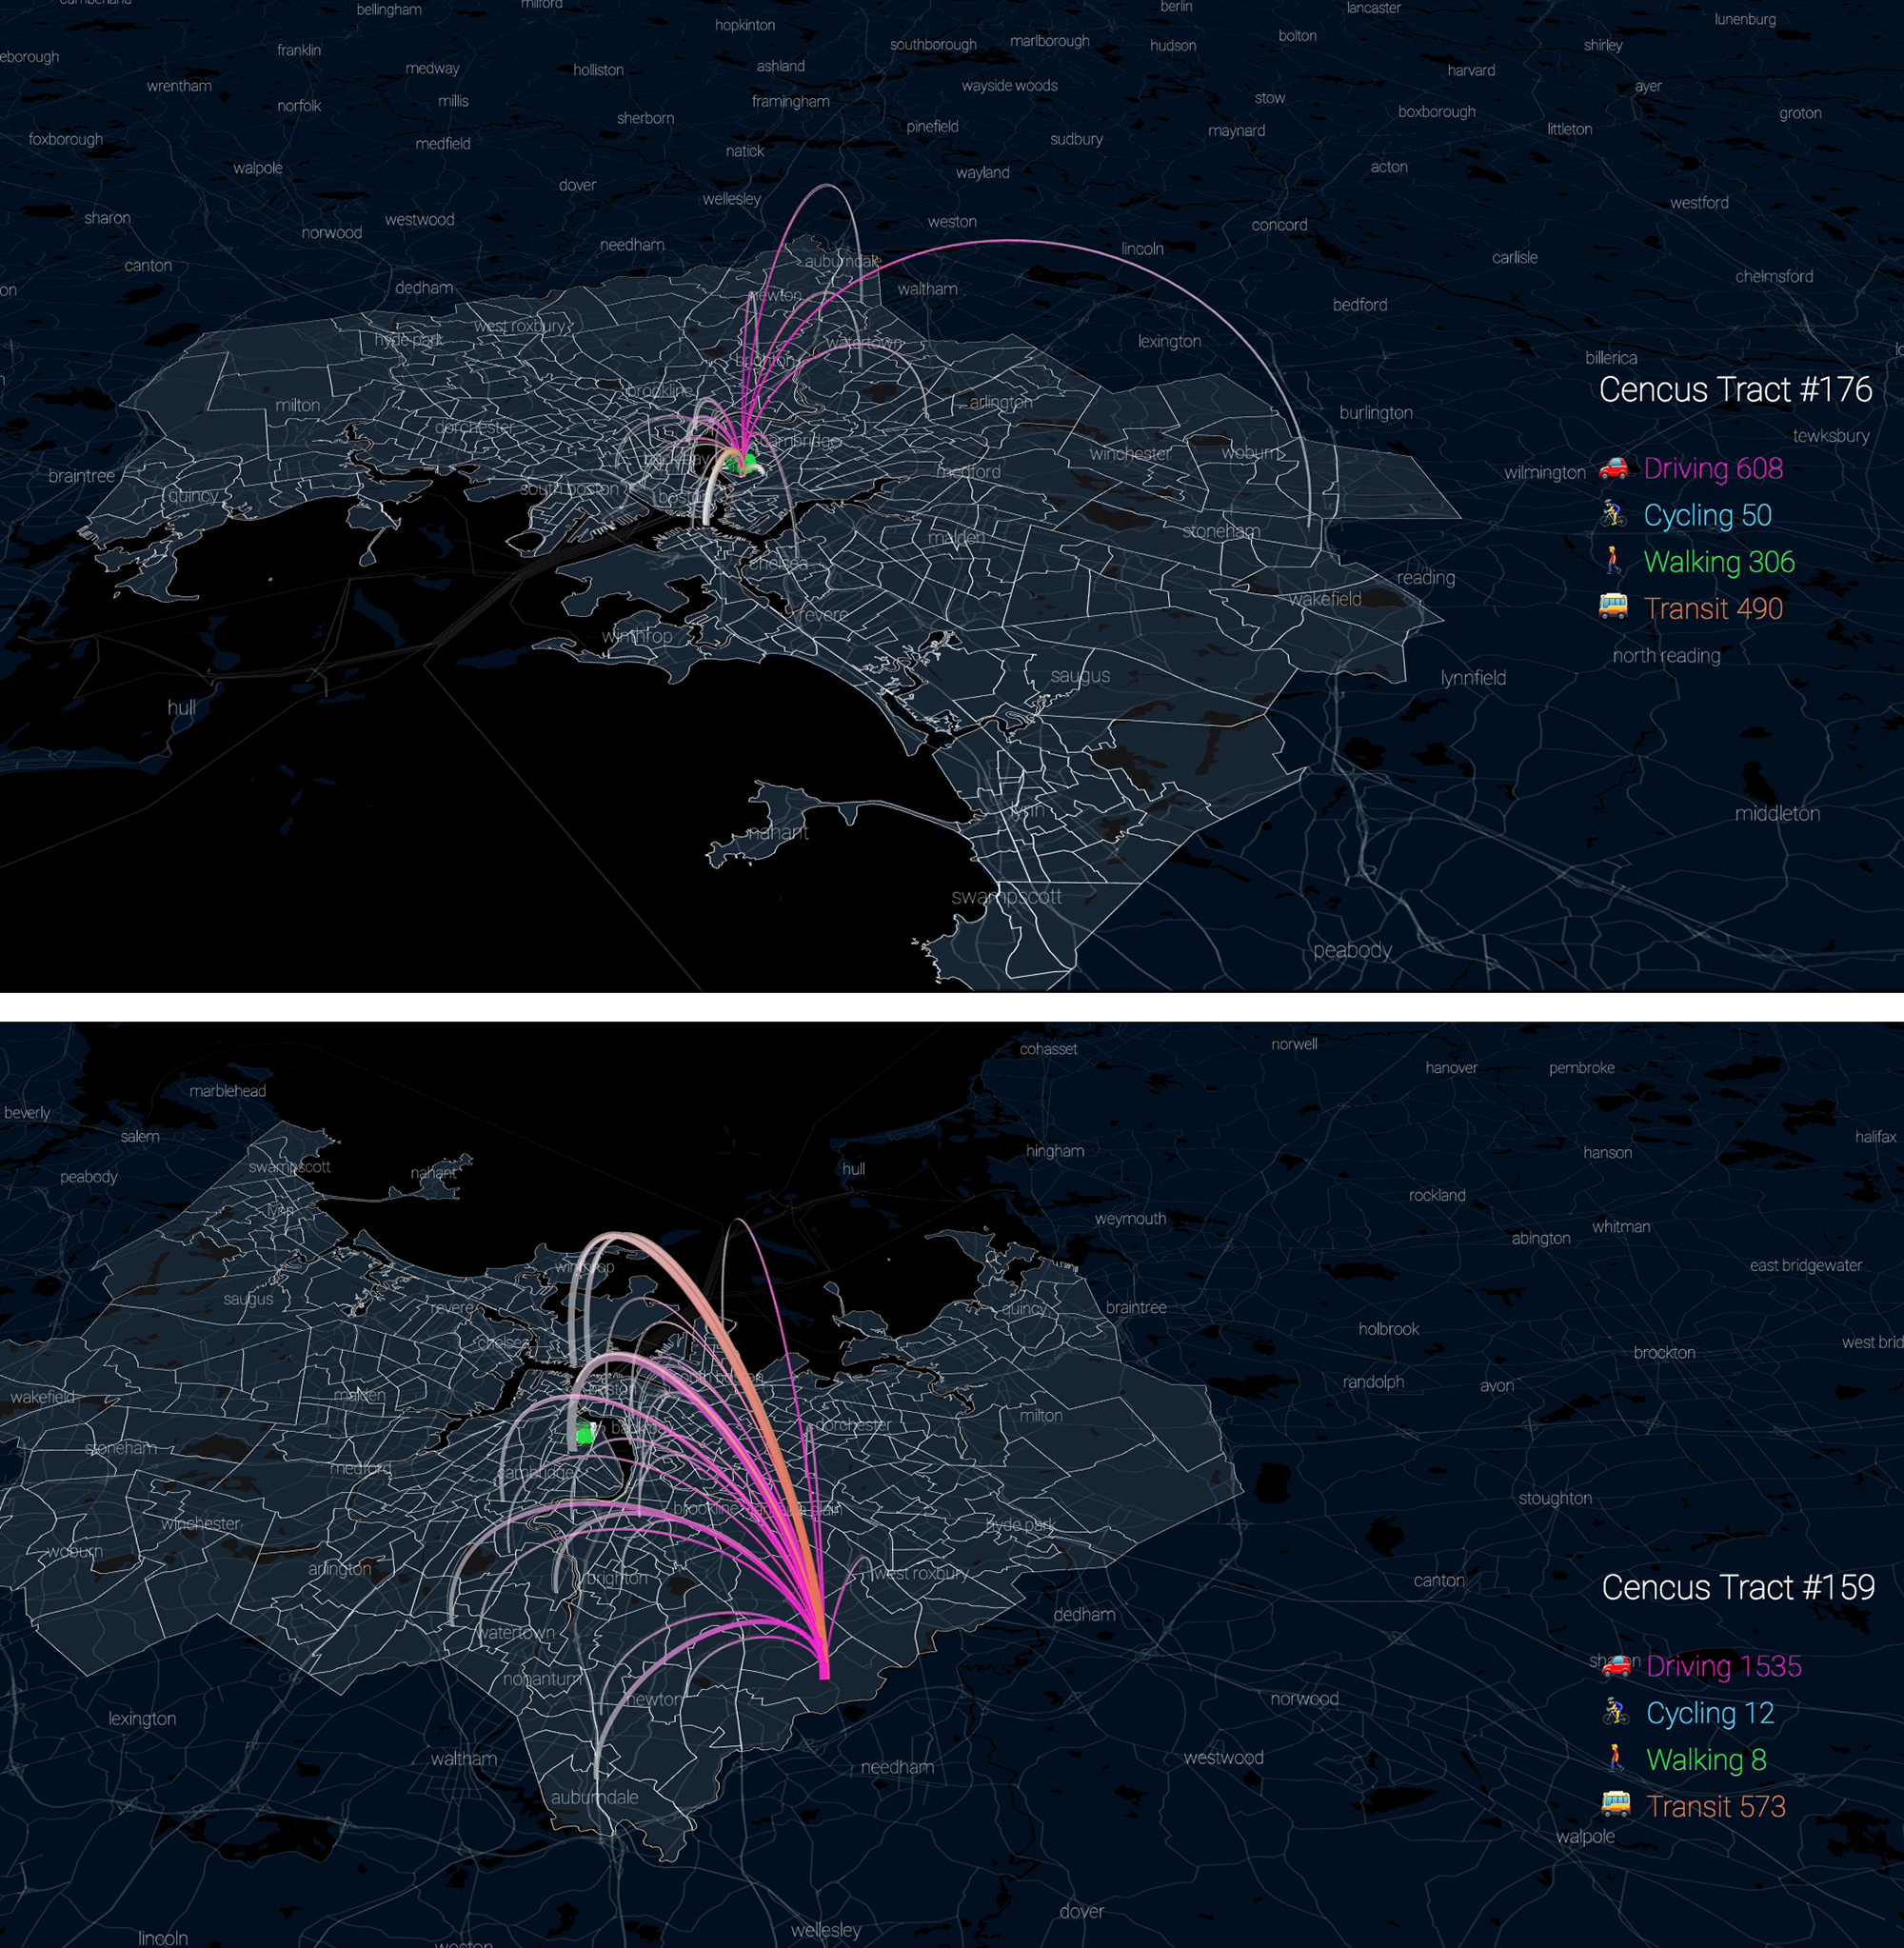
\includegraphics[width=.9\linewidth]{chapters/prediction/mocho/figures/mocho3.png}
            \caption{MC predictions}\label{fig:mocho_arcs}
            \caption*{MC model results. (top) shows trips originating at the Volpe site census tract and (bottom) showing trips from a suburban tracts. The arcs display volumes of trips (thicknesses) between each O-D pair for each mode (color). As clearly shown, the suburban tract yields more car trips with greater distances than those originating at the Volpe site.}
        \end{figure}


        \subsubsection {Feedback}
        {
            This feedback component shows data from the MC model, the scanned TUI and a Geo-data service. The Geo-data service serve census tract data of the Greater Boston Area via \verb|GEOJSON| polygons, projected onto a cartographic background. Than, the results of the MoCho model are rendered as origin-destination (O-D) arcs connecting pairs of different census-tracts, as shown in Figure \eqref{fig:mocho_arcs}. Each arc represents the sum of trips between the pair of tracts, with color representing the prevailing MC chosen by most trips leaving that tract (i.e., green for bikes, purple for cars, etc.). The arc's thickness corresponds to the sum of trips by that mode. On average, nearly 11,000 arcs are reproduced with each user iteration; To avoid illegibility and visual noise, the UI renders only arcs terminating at a given census tract, selected via user's interaction. For each selected census tract, the breakdown of trips by each mode also displayed in numerical format. The UI was built and deployed as a web application, using the ReactJS \cite{react}, Mapbox GLJS, and DeckGL \cite{deckgl17:online}.
        }

        \subsubsection{MoCho TUI}
        {
            The MoCho TUI is used as the design space and a canvas for visualization. With each user interaction, the canvas updates a schematics land-use diagram, representing the Volpe development site. A shadow mapping algorithm adds perceptual depth to the grid tiles so that higher density tiles appear taller than others. A background mapping service contextualizes the design space to the site, in this case Volpe area. Lastly, animated color dots represent individual trips entering or exiting the site, as they are inferred from the MoCho model. The dots colors correspond to the mode-choice arcs on the vertical display (i.e., a purple dot is one vehicular trip) and animated to move from general direction of that tract to its designated land-use destination.
            \newline
            A more advanced version of this simulation assigns trips to routes based on Dynamic User Equilibrium or micro-simulation, and feed updated travel times back to the mode-choice predictions. This simulation was introduced to the CityScope Grasbrook \eqref{sec:grasbrook} and later in the CityScope Corktown project in Detroit, MI. Together, the feedback modules assist users to associate the relatively small-scale urban development with metro-scale MC impacts.

            \begin{figure}[!htb]
                \centering
                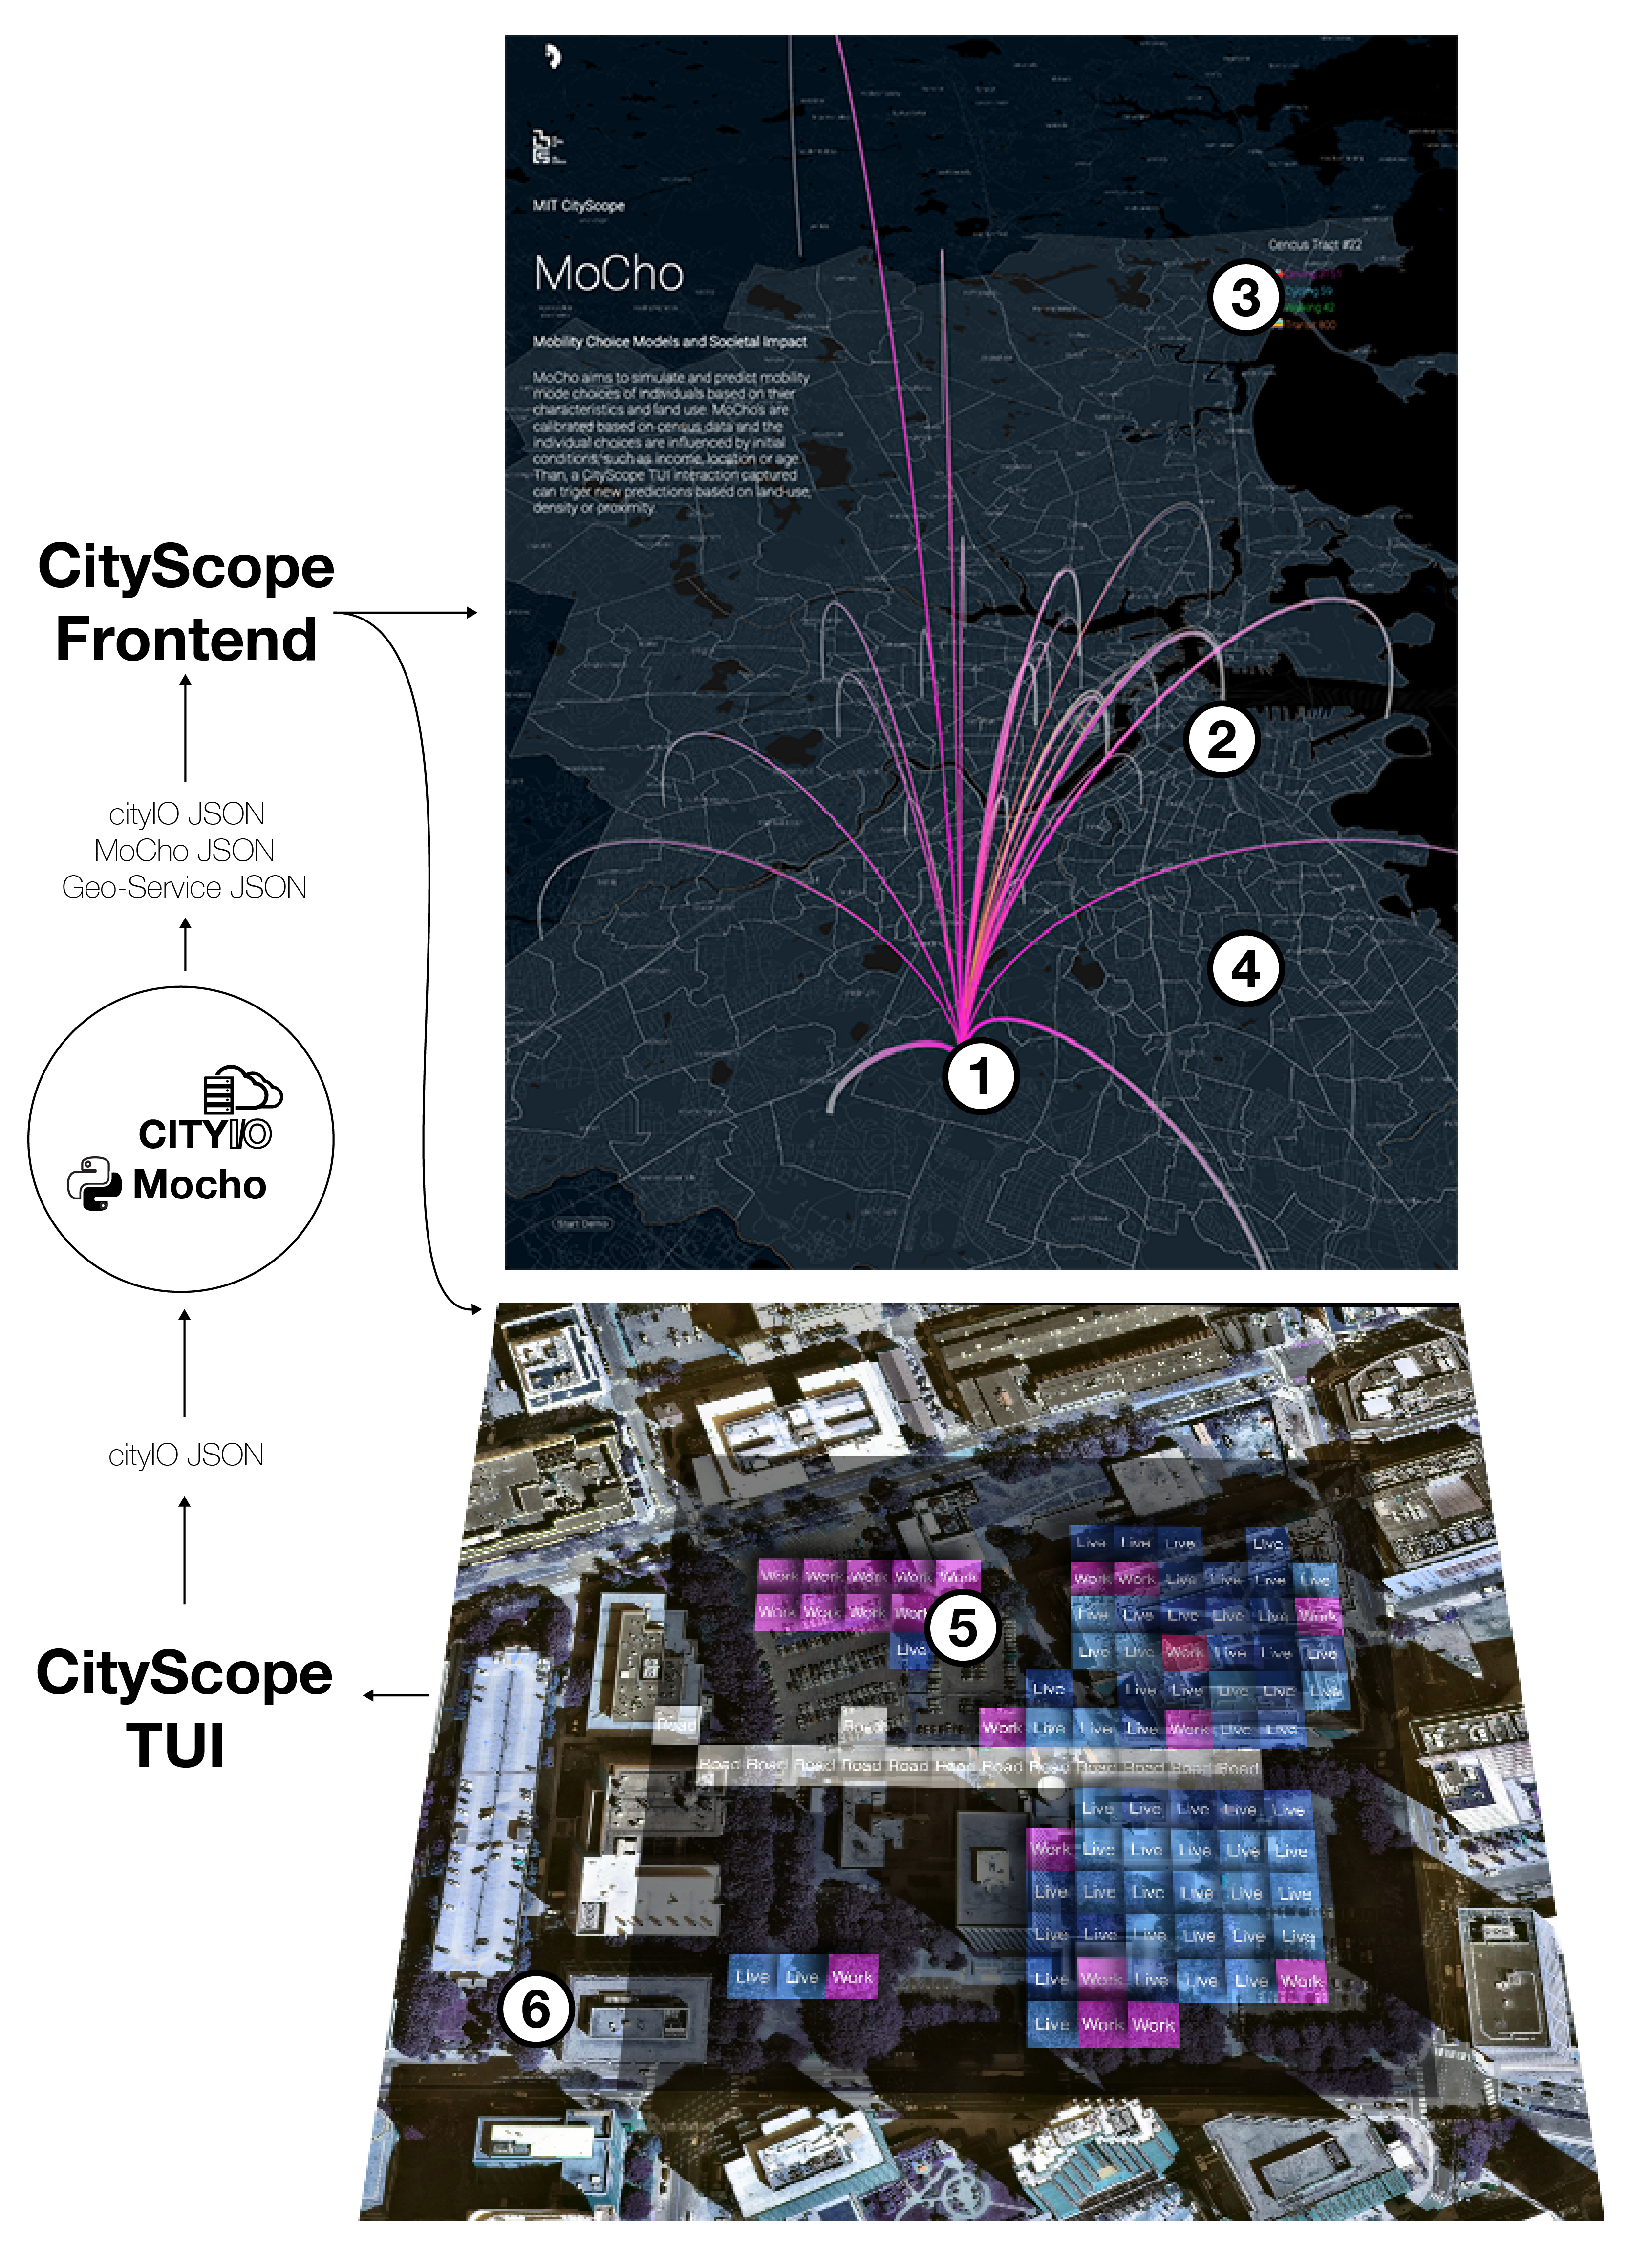
\includegraphics[width=0.65\linewidth]{chapters/prediction/mocho/figures/mocho1.jpg}
                \caption{CityScope MoCho Interface Components}\label{fig:mocho_components}
                \caption*{Vertical Display: (1) Selected tract showing trips and their MC (2) MC trip ending at the Volpe site (3) Numerical output of tract's MC (4) GeoJson of ~500 computed census tracts. Horizontal TUI: (5) Tagged LEGO bricks with projected land-use scheme (6) Immediate context surrounding the Volpe site design space}
            \end{figure}

        }

        \subsubsection{Model Calibration Results}
        {
            The mode-choice model introduced in Section \eqref{sec:mocho-models-data} must be calibrated for each location context; For the Volpe Case Study, data for the Boston metro area were used. Through some exploratory analysis of Boston's PUMS data, a number of variables were selected as being likely to affect MC. As well, some features were converted to different formats. For example, the age and income variables were converted from continuous to binary variables by dividing each into three quantiles and using binary variables to indicate records in the lowest and highest groups.
            \newline
            The encoding of travel-time also required some experimentation. Time spent in different types of travel activities, such as driving, waiting for a bus or walking, are associated with different perceived costs and therefore should be treated differently in discrete choice models, without being too specific which can cause model under-fitting. In this case study, it was found that using the three variables of \verb|walking\_time|, \verb|cycling\_time| and \verb|in\_vehicle| led to a well fitted model with sensible parameter estimates.
            \newline
            The final model had a pseudo-R-squared value of 0.45 which indicates a well fitting model. The full list of parameters estimates is shown in Appendix Table \eqref{appendix:mocho-tab-results}. When interpreting the parameters, it should be noted that the choice of driving was taken as the reference choice. For example, all of the parameters for the density variables are positive, indicating that increases in residential or employment density in one's home or workplace, are associated with increased likelihood of cycling, walking or public transit relative to driving. The travel-time parameters show that time spent cycling is perceived as the most costly whereas time spent in vehicles is the least costly, which is in line with prior research \cite{koppelman2006self}. Finally, some societal and cultural associations are found between personal characteristics and the likelihood of taking each mode. For example, the model shows that having a college degree, a graduate degree and/or working for a non-profit, decreases one's likelihood of driving and in particular, increases one's likelihood of taking active modes. Also, those in the youngest age group and lowest income group are less likely to drive than others.
        }
    }
    \subsection{Discussion}
    {
        CityScope MoCho was designed to bridge the gap between smilingly minor changes to the built environment, and behavioral choices of individuals in remote locations. It was achieved by predicting mobility choices (MC) and societal impacts in response to user inputs through the CityScope TUI. While there already exist tools for predicting MC and environmental impacts of transportation, few efforts have been made to integrate these modeling steps in an end-to-end real-time, and collaborative tool.
        The underlying models were well calibrated using publicly available data sources, ensuring the credibility of the model predictions; Similar models could be created for other urban areas with minor adaptations to the underlying model.
        \newline
        Moreover, using these models for prediction, typically requires laborious specification of inputs by professionals. The platform developed here provides an intuitive user-interface to such models, allowing multiple people with varying levels of expertise to collaboratively experiment with different urban-designs scenarios and real-time feedback. MoCho has advanced the CityScope architecture with on-demand pre-trained models, a distributed computational backend, and an online user interface which was a precursor to CityScopeJS (see Section \eqref{sec:cityscope_architecture}); many of these ideas evolved into the current CityScope platform.
    }
}
    %%%%%%%%%%%%%%%%%%%%%%%%%%%%%%%%%%%%%%%%%%% 
    \section{DeepScope: A Deep Image of the City}\label{sec:deepscope}

{
    \subsection{Introduction}
    {
        As discussed in previous sections, predicting the impacts of city-planning can help evaluate the future performance of different urban systems - from mobility and energy to safety and economic development (see Sections \eqref{sec:cityscope_volpe}, \eqref{sec:grasbrook}, \eqref{sec:modeChoices}). Nevertheless, more subtle aspects of planning, such as the physical appearance of development, are not easily predicted or evaluated during early planning stages.
        \newline
        Urban-design renderings and streetscape visualizations are commonly used by designers, stakeholders, and decision-makers to asses future design. These visual aids can clarify the outcomes of design decisions, such as zoning, building codes or land-use allocations, and can affect urban development for decades to come \cite{al1999using, smith1998visual}. Yet despite major advancements in computer graphics, rendering, and visualization tools, crafting quality urban visualizations is still a complex, lengthy and costly task. This work introduces \textit{DeepScope}, a CityScope module for real-time urban-design visualizations. DeepScope utilizes a Generative Neural Network (DCGAN \cite{mirza2014conditional}) designed for real-time feedback. The rest of this section details the design and the implementation of DeepScope.

        \subsubsection{`Imageability'}
        {
            \emph{``To understand the role of environmental images in our own urban lives (...) we needed to develop and test the idea of imageability (...) and thus to suggest some principles for urban-design.''} \cite{lynch1960image}


            \begin{figure}[!htb]
                \centering
                \includegraphics[width=1\columnwidth]{chapters/prediction/deepscope/figures/deepscope5.png}
                \caption{Urban `Imageability'. (left) Kevin Lynch's imageability classification metric for street element and urban experience. (right) An example street view, in which many of these classes are homogeneously interconnected \cite{lynch1960image}.}~\label{fig:deepscope_lynch}
            \end{figure}

            In 1960, MIT professor and Urbanist Kevin Lynch, introduced the idea of urban `imageability': a novel approach to visual perception of the built environments \cite{lynch1960image}. Lynch suggested a new classification of city-form, in which nodes, landmarks, paths, edges and districts reflect the sensation of traversing through the urban scape. Figure \eqref{fig:deepscope_lynch} demonstrates Lynch's imageability  and their manifestation in the streetscape. In the 1964 `The View From the Road' study \cite{appleyard1964view}, Lynch tested the idea of `imageability' using a new medium: He mounted a film camera to a car dashboard, and went on several day rides around five US metros \cite{Andrews2007}. When later played, these recordings were sped to reflect the overall `feel' of the urban skyline, overlooking nuanced street elements and architectural details, and prompting questions such as: What is the composition of the built mass? What shapes the street-section? Are there any noticeable landmarks, forms, or gaps? \cite{carr1969city, pearce1996legacy}.
        }

        \subsubsection{Urban Visualization}
        {
            Lynch's work contributed to the notion that street-level views are critical during initial urban-design stages, when the urban context is only being established \cite{drettakis2007design, brusaporci2017importance}. In the last few decades, advancements in computer graphics made it easier to visualize future urban developments \cite{shiode20003d, kempenaar2016design}. Nevertheless, few tools provide realistic and real-time urban visualizations, which can also be used as part of collaborative design processes \cite{mueller2018citizen}.
            \newline
            Most common visualization tools carry complex setups, costly hardware and software, as well as steep learning curves \cite{yan2014evaluation, mekni2014augmented}. These tools often require users to set up many control parameters, such as cameras, lights, and materials, and constantly adjust these to produce decent results. This process can become laborious in complex design scenes, and can gravely affect the outcome, cost and duration of visualization processes, and the design process as a whole \cite{lovett2015using}.
        }
    }


    \begin{figure}[!htb]
        \centering
        \includegraphics[width=1\columnwidth]{chapters/prediction/deepscope/figures/deepscope3.png}
        \caption{From interaction to prediction. (left) TUI interactions are captured using OpenCV and streamed to the webGL app. A 3D model is created based on the grid's JSON array and the Observer viewing angle. Lastly, a snapshot image is fed as an input vector to the DCGAN model. (right) (1) Observer position (2) Observer view angle and FOV cone (3) Observer's 3D street-view as input for DCGAN (4) DCGAN model prediction of street-view (5) TUI interactive grid.}~\label{fig:deepscope_dataflow}
    \end{figure}



    \subsection{System Design}\label{DeepScope-system-architecture}
    {
        DeepScope is a CityScope module for collaborative, tangible, and real-time urban-design visualization. DeepScope allows multiple users to collaboratively observe the visual outcomes of early planning stages using autogenerated visualizations. As with other CityScope platforms, DeepScope requires minimal setup, basic hardware and software, and no expertise to use\footnote{For general design of CityScope platforms see Section \eqref{sec:cityscope_architecture}}.

        \subsubsection{DeepScope User Interaction}\label{DeepScope-user-interaction}
        {
            DeepScope TUI is composed of three components: (i) A physical urban model, (ii) a scanning module, and (iii) a feedback module. The urban model includes an arbitrary grid of LEGO tiles, tagged with binary patterns, and scanned using CityScoPy as discussed in Section \eqref{subsec:csarch-cityscopy}. Figure \eqref{fig:deepscope_users} depicts a user positioning a tagged LEGO brick into the TUI design space to trigger the model generation.

            \begin{figure}[!htb]
                \centering
                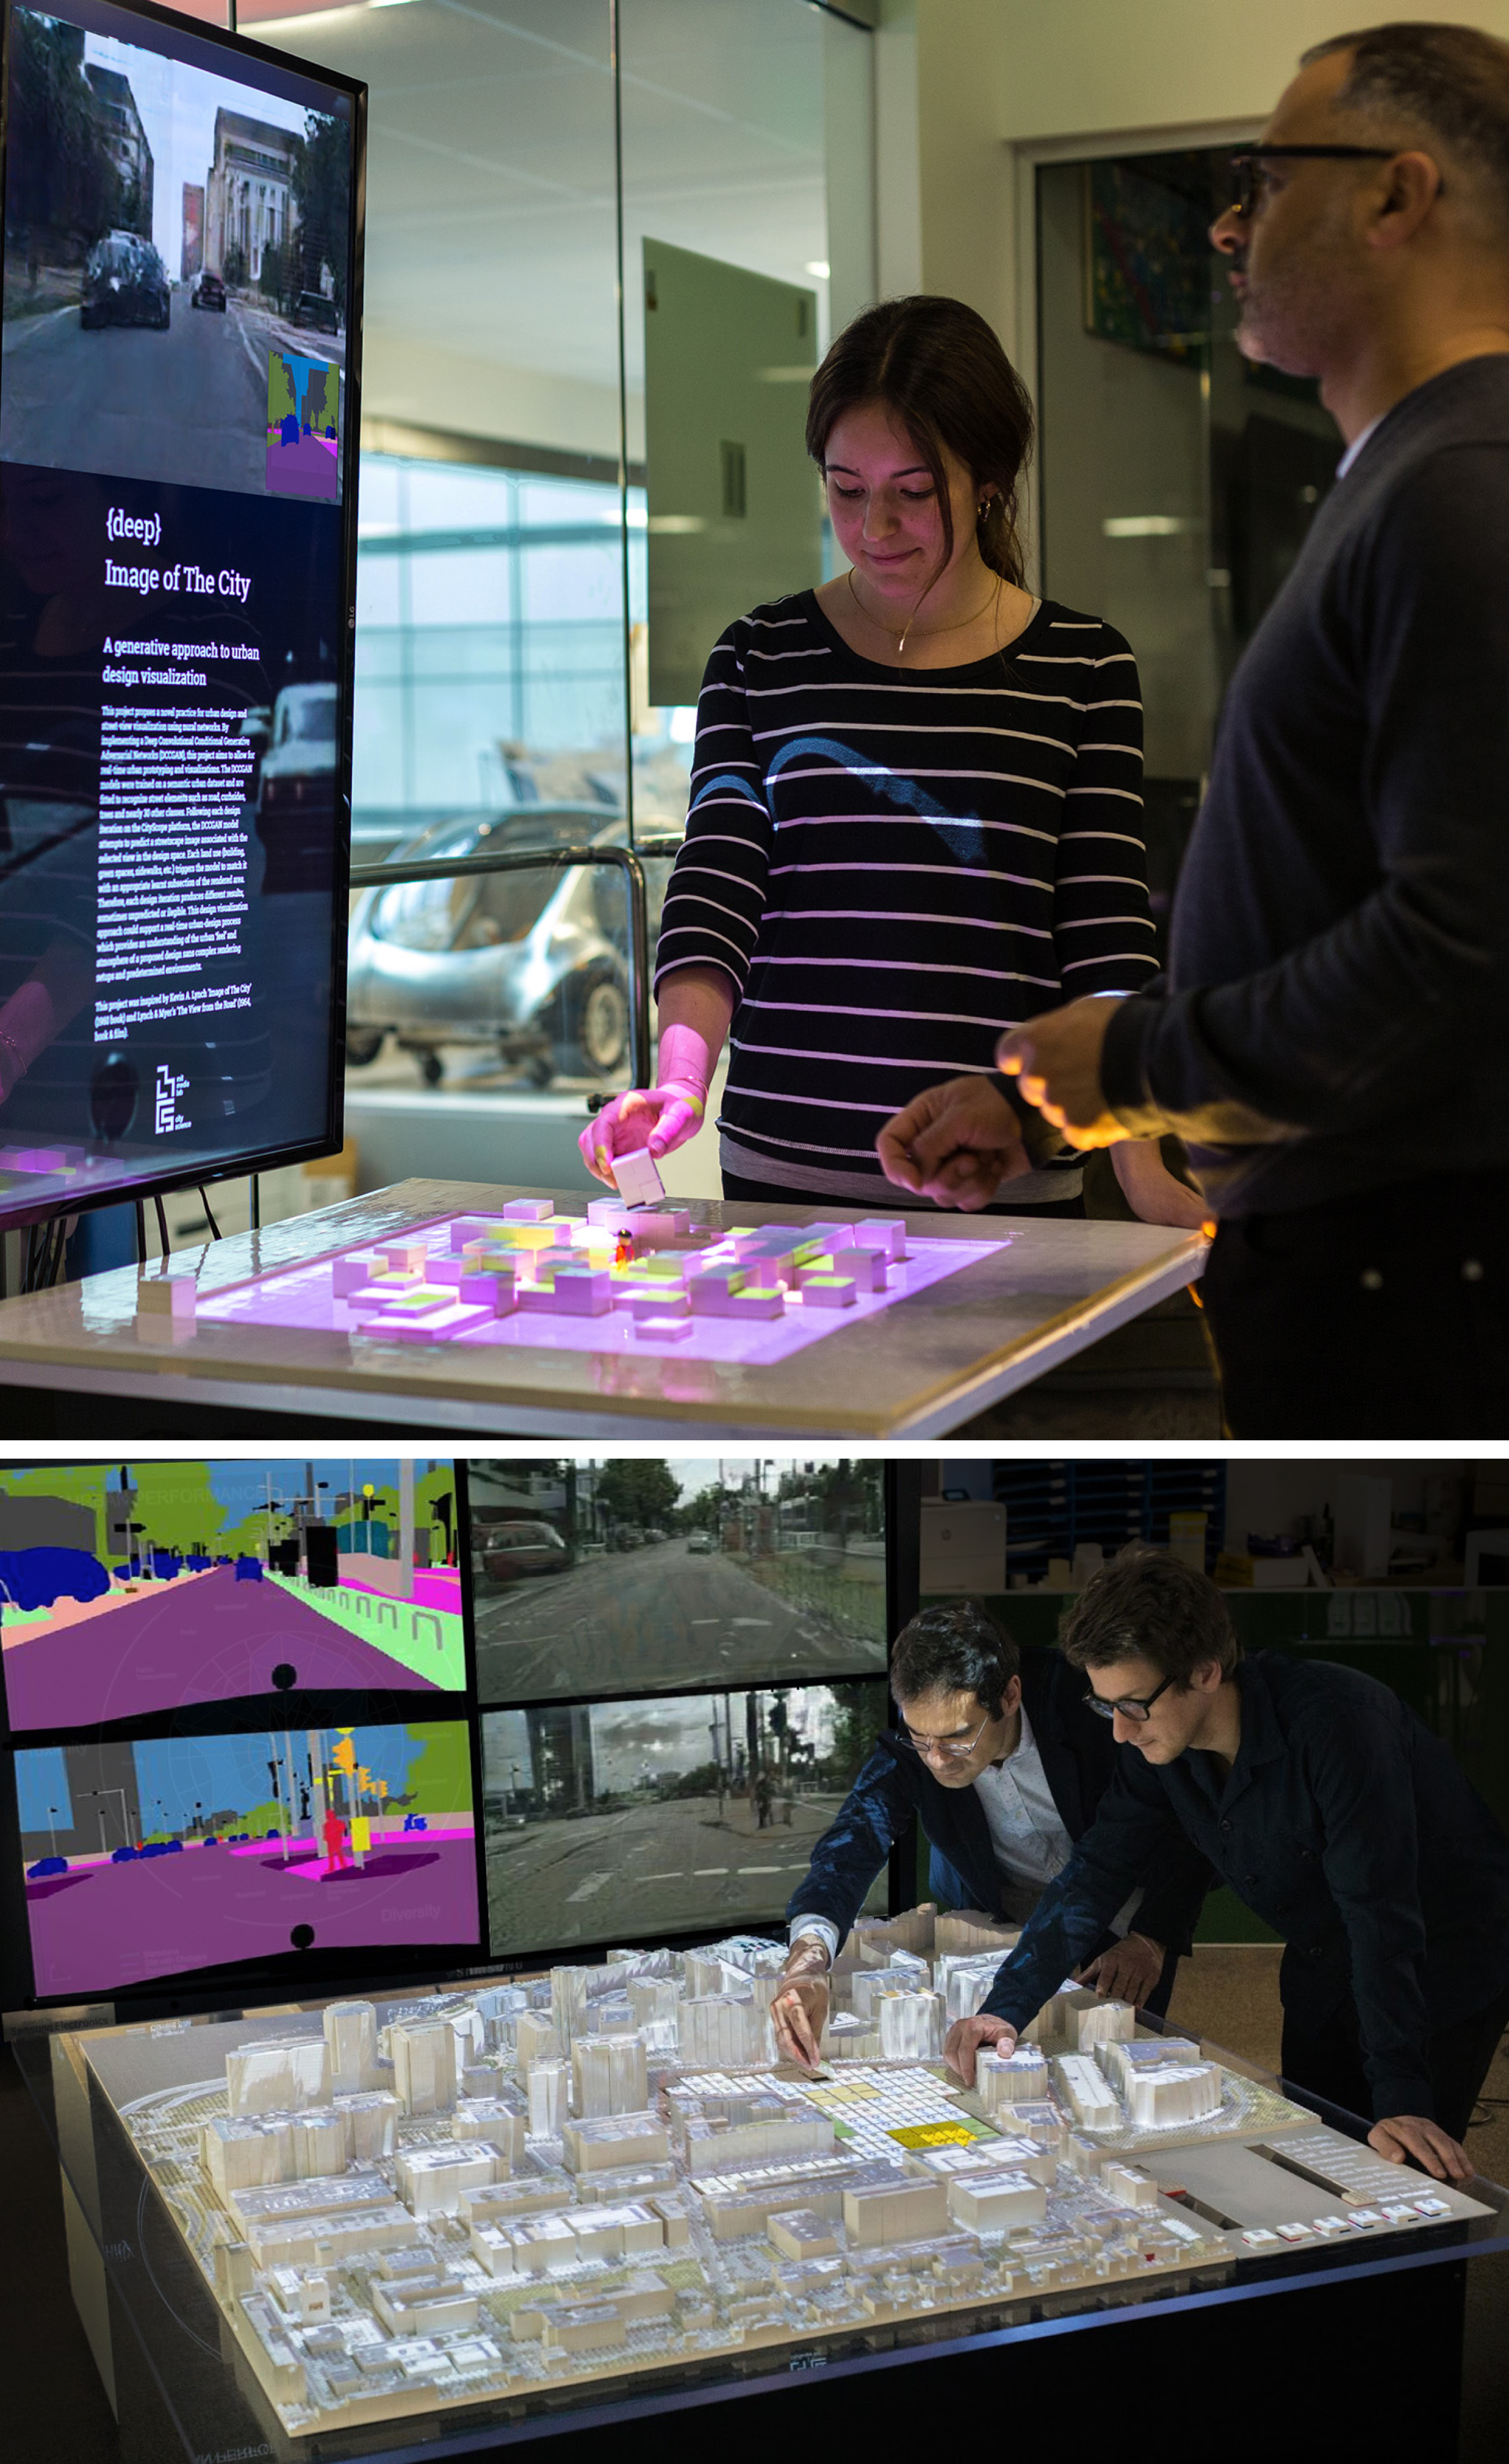
\includegraphics[width=0.6\columnwidth]{chapters/prediction/deepscope/figures/deepscope2.png}
                \caption{
                    Multi-user interaction with DeepScope.
                    Multiple users can simultaneously interact and discuss urban-design iterations. The table-top is used as both the design space and a schematic urban top-view. The vertical monitor visualizes the DCGAN street view.
                }~\label{fig:deepscope_users}
            \end{figure}

            In DeepScope, each grid-cell pattern represents a different streetscape class, such as roads, buildings, green-spaces, parking, or sidewalks. Each class contains additional parameters, such as height, volume, shape, rotation and density. Table \eqref{deepscope:tab-types-classes} specifies the classes and their attributes.


            \begin{table}
                \begin{center}
                    \caption{
                        Cityscapes dataset classes used in DeepScope. Marked with `plus' are labels which can be altered dynamically using CS TUI. Marked with `star' are labels that are generated dynamically in the 3D model.
                    }
                    \label{deepscope:tab-types-classes}
                    \begin{tabular}{l|l}
                        \hline
                        \textbf{Group} & \textbf{Classes}                                                     \\
                        \hline
                        flat           & road*+; sidewalk*+ parking*+; rail track                             \\
                        human          & person*; rider*                                                      \\
                        vehicle        & car*; truck*; bus*; on rails; motorcycle; bicycle*; caravan; trailer \\
                        construction   & building; wall*; fence; guard rail; bridge                           \\
                        object         & pole*; pole group; traffic sign*; traffic light*                     \\
                        nature         & vegetation*+; terrain                                                \\
                        sky            & sky*                                                                 \\
                        void           & ground; dynamic; static
                    \end{tabular}
                \end{center}
            \end{table}
        }

        \subsubsection{Procedural Environment}
        {
            With each user interaction, the scanner decodes the array of grid-cell patterns and updates the CityScope Schema (see Section \eqref{sec:cityscope_architecture}). This triggers a generation of a virtual 3D environment, in which each grid-cell is represented via its class and additional parameters (see Figure
            \eqref{fig:deepscope_dataflow}
            ). As users allocate tiles, the 3D environment is procedurally populated with streetscape elements. For example, a vegetation pattern will create a surface with procedural trees, bushes or live-fences; A sidewalk pattern will produce pedestrians and street-signage, and a parking-lot pattern will be proliferated with parked vehicles. The generated 3D environment is uniformly hued with RGB values that correspond to input classes which correspond to the Cityscape dataset classes, and are expected by the GAN model (see Section \eqref{DeepScope-Generative-Model}). The 3D scene generation is done on the client-side web-browser using WebGL and ThreeJS \cite{mrdoob_2019}.
        }


        \begin{figure}[!htb]
            \centering
            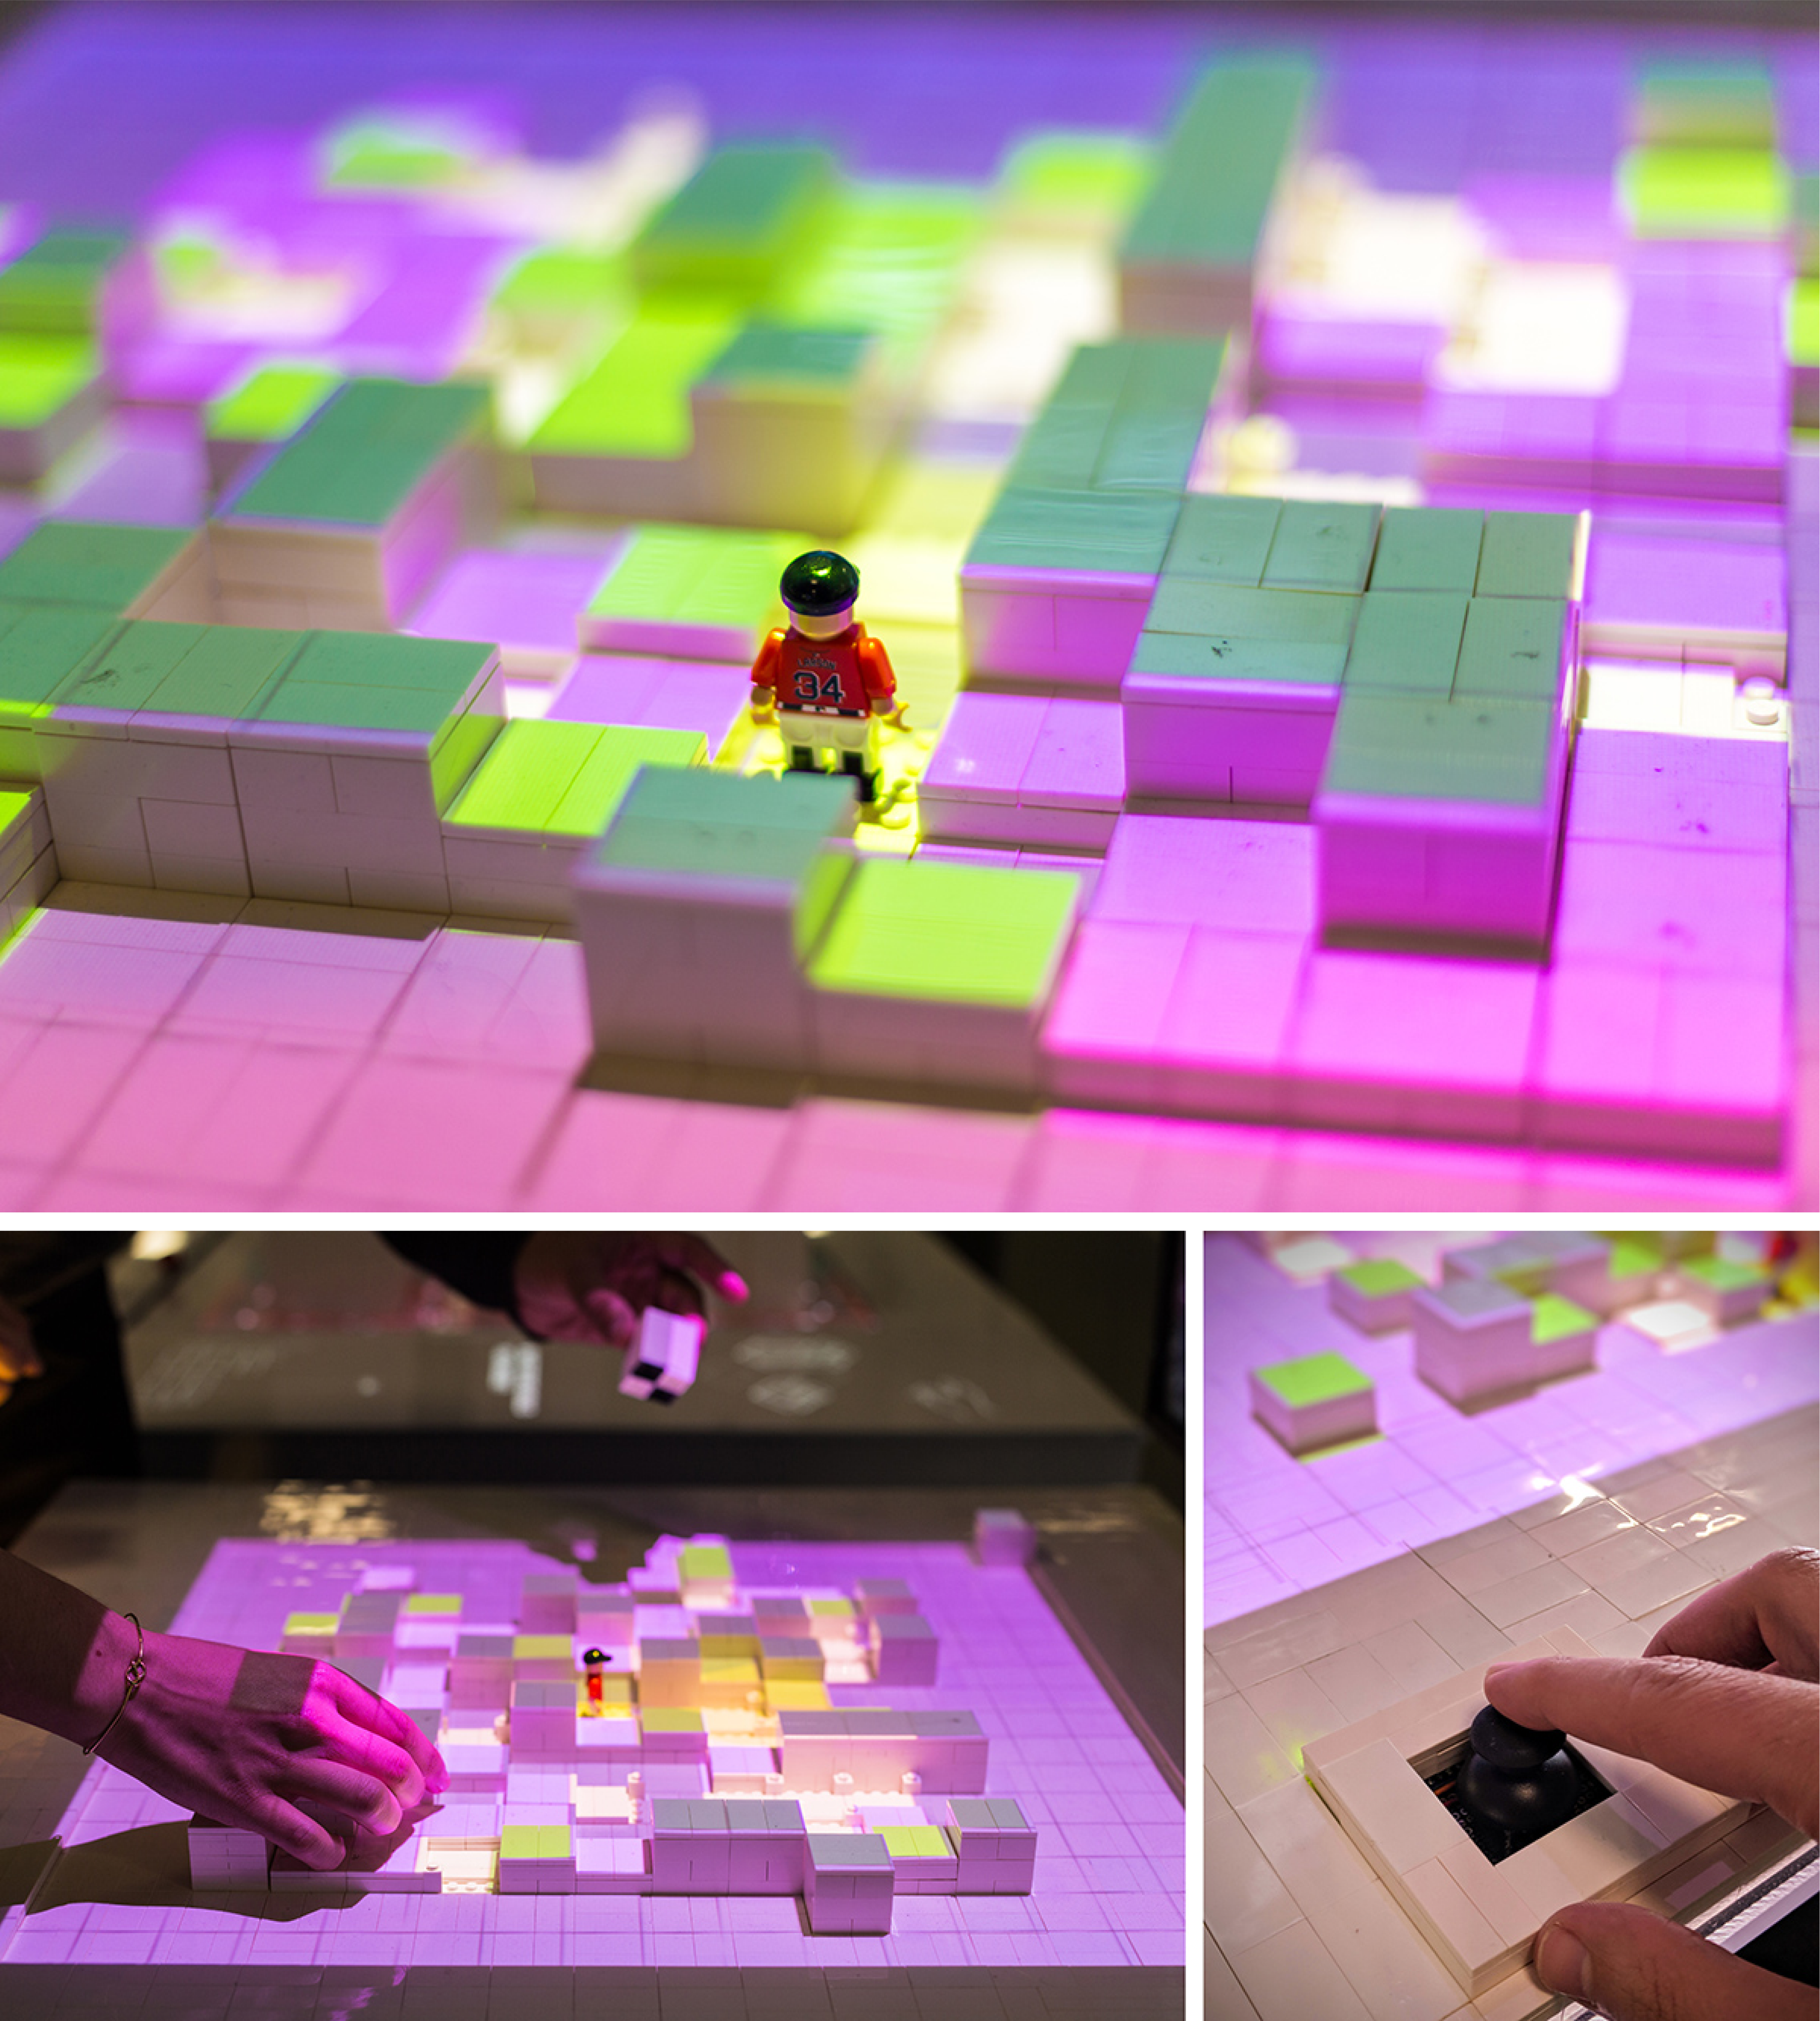
\includegraphics[width=0.7\columnwidth]{chapters/prediction/deepscope/figures/deepscope4.png}
            \caption{DeepScope TUI. (top) TUI and the Observer tile. (left) User interaction with grid-cells. (right) `Observer' viewing angle, depth and position is set via an Arduino game-pad}~\label{fig:deepscope_observer}
        \end{figure}


        \subsubsection{Observer}\label{observer}
        {
            The urban environment designed by the users is constantly captured by the `Observer' grid-cell. Similar to Lynch's `View form the Road' \cite{appleyard1964view}, this one-off unique CityScoPy pattern, mimics a virtual nomad traversing through the city. The Observer allows users to sets the position, point-of-view and angle of a virtual camera in the 3D scene, so that real-time visualizations will be predicted from that view. The Observer baseline parameters (such as FOV, Frustum and camera-height) were approximated to the camera calibration appendix of the Cityscapes dataset used in model training \cite{Cordts2016}. Additional camera controls were implemented to allow users to move, rotate, pan or zoom the Observer via custom game-pad joystick (see Figure \eqref{fig:deepscope_observer}).
        }

        \subsubsection{Tabletop Feedback}\label{deepscope-table-top}
        {
            As with other CityScope instances, DeepScope tabletop is used as both the design space and a canvas for data visualization. With each design iteration, an illuminated land-use diagram is projected onto the table-top, so that each tile is showing its respective pattern, name or parameters (density, land-use, etc.). The Observer position is displayed using perspective cone that indicates its current viewing angle and FOV (see Figure \eqref{fig:deepscope_dataflow}).
        }
    }

    %%%%%%%%%%%%%%%%% GAN  %%%%%%%%%%%%%%%%%% 


    \begin{figure}[!htb]
        \centering
        \includegraphics[width=0.5\columnwidth]{chapters/prediction/deepscope/figures/deepscope6.jpg}
        \caption{From site to prediction. This process depicts site selection, conversion to CityScope Schema, interaction, and prediction using the DCGAN model.}
        \label{fig:deepscope_pixelation}
    \end{figure}

    \subsection{Generative Model}\label{DeepScope-Generative-Model}

    {
        DeepScope uses a Deep Convolution Generative Adversarial Network (DCGAN) in order to generate street-view visualization in real-time. With each TUI interactions, the Observer viewpoint is captured as an input vector, used by the DCGAN model to predict an image (see Figure \eqref{fig:deepscope_dataflow}). The DCGAN generates an bitmap corresponding to the input vector, where each pixel in the input vector triggers the prediction of a corresponding pixel in the DCGAN output. The resulting image is then drawn onto the DeepScope feedback module.
    }

    \begin{figure}[!htb]
        \centering
        \includegraphics[width=1\textwidth]{chapters/prediction/deepscope/figures/deepscope0.jpg}\caption{(Top row) Model trained on Cityscapes dataset, deployed as node.js app. (Bottom row) TUI triggers DCGAN renderings.}~\label{fig:deepscope_arch}
    \end{figure}

    \subsubsection{Dataset and Model Training}\label{model-and-data}
    {
        Accurate pattern recognition using neural networks (NN) was already possible in the late 1980's \cite{lecun1989backpropagation}. However, generating new data that well concatenates a given dataset is still considered a complex problem in Machine Learning \cite{creswell2018generative}. Data generation using NN was greatly advanced with the introduction of Generative Adversarial Networks (GAN) \cite{Goodfellow2013}. GAN use two competing NN, a Generator and a Discriminator, that `adverse' one another; The Generator attempts to create new data (such as image, sound or text), and the Discriminator aims to nullify these data by comparing them to the distribution of a ground-truth data. The training is usually completed when the Generator can create close to indistinguishable samples which can fail the Discriminator \cite{pix2pix2016}.
    }


    \subsubsection{Image-to-Image Translation}\label{image-to-image-translation}

    {
        A variant of GAN is Conditional GAN (CGAN), in which both NN are given additional data that focuses the generation on specific targets \cite{mirza2014conditional, salimans2016improved}. A notable use-case of CGAN is a pixel-wise conditional generation of images, known as Image to Image Translation or `pix2pix' \cite{isola2017image, pix2pix2016}. In pix2pix, pairs of images are used for training, where the pixel values of one image are used as labels (also known as `classes') of the other. This allows pixel-level prediction using spatial classification of regions in the image \cite{arjovsky2017wasserstein, zhu2017unpaired}. In practice, CGAN extends the classic GAN zero-sum objective function with additional class data so that:
        \begin{equation} \label{deepscope-gan-objective-function}
            \min_G \max_D V(D, G) = \mathbb{E}_{\bm{x} \sim p_{\text{data}}(\bm{x})}[\log D(\bm{x} | \bm{y})] + \mathbb{E}_{\bm{z} \sim p_z(\bm{z})}[\log (1 - D(G(\bm{z} | \bm{y})))]
        \end{equation}
        where function ${V}$ of the Generator and the Discriminator ${G, D}$ attempts to minimize a delta between ground-truth data ${x}$ (in this case, the pixel data) and ${z}$, which is the accumulated pixel distribution learnt on each training step (see Figure \eqref{fig:deepscope_epoch}). Unlike classic GAN, $\log_{D(\bm{x} | \bm{y})}$ denotes that the additional `class' data ${y}$ conditions the learning on both data \textit{x} as well as on ${y}$ class. In this respect, CGAN generator do not only generate data with resemblance to the learnt distributions, but can closely mimic details in the data structure. DeepScope implements a variant of pix2pix that is fast and lightweight enough for real-time predictions in web browsers of low-tier devices.
    }


    \subsubsection{Cityscapes Dataset}\label{cityscapes-dataset}
    {
        The DeepScope DCGAN model was trained on the Cityscapes dataset \cite{Cordts2016}. Cityscapes is composed of pairs of street-view images taken using a dashcam around 50 European cities, during different seasons, daytime and weather conditions. Each pair includes a street-view image and a corresponding segmented image with 30 semantic labels (`classes'). These labels represent different streetscape classes, from buildings and roads to license-plates and road signs. For DeepScope, a pre-processing algorithm was designed to remove motion-blur, increase sharpness, saturation and remove color-casting, which were common in a shots taken by a moving vehicle. This pre-processing tools was built in Python OpenCV \cite{opencv_library}.

    }

    \subsubsection{Model Architecture and Performance}\label{dCgan-model-architecture-and-performance}
    {
        The model architecture of DeepScope was designed to allow fast predictions and portability for web-based devices. The Generator network has 16 layers with a U-Net encoder-decoder structure \cite{ronneberger2015u}. For performance purposes, the Discriminator has only 5 layers and is using Leaky ReLU activation that has been shown to improve stability in training \cite{Radford2015}. Commonly, DCGAN models benefit from higher number of filters \cite{ronneberger2015u}, however more filters also increase the model size, which can impact real-time performance and usability in low-tier devices. In order to still maintain attention to fine details, a shallow network design with a random up-sampling of 150\% was used \cite{isola2017image}. This network allows deployment on client-side browsers or mobile devices where TensorFlowJS is supported \cite{smilkov2019tensorflow}.
    }



    \begin{figure}[!htb]
        \centering
        \includegraphics[width=0.3\columnwidth]{chapters/prediction/deepscope/figures/deepscope1.jpg}
        \caption{Test samples during training. Right column shows quality degradation beyond $\sim$200 epochs.}~\label{fig:deepscope_epoch}
    \end{figure}


    \subsubsection{DCGAN Training and Results}\label{dCgan-training-and-results}
    {
        20 training sessions were conducted with 16, 32, 64 and 128 filters, and 50 to 2000 epochs. Resulting models were converted to a \verb|JSON| format and tested for stability and response time on various browsers. A trained model with 64 filters and 200 epochs showed the best overall results. Models with less filters produced low-quality results; models with up to 2000 epochs demonstrated inconsistencies and `mode collapse' \cite{arjovsky2017wasserstein}.
    }


    \subsubsection{UI Performance Test}\label{deepscope-platform-and-user-interaction}
    {
        In order to avoid interaction latency, two asynchronous processes were used: (i) prediction process, and (ii) TUI interaction response. In user tests, the DCGAN model predicted at $0.66 sec/prediction$ on an average desktop system used by CityScope instances; the TUI has a fixed response interval of 50ms. Although DCGAN predictions slightly trails the TUI, the observation showed that users tend to focus their attention to the horizontal TUI before expecting the DCGAN output. Therefore, the overall user experience could be considered real-time with continuous design-and-feedback loops \cite{deber2015much}.
    }


    \subsection{Discussion}\label{deepscope-discussion}
    {
        DeepScope is a CityScope module which uses a real-time neural-network model to provide early stage urban-design visualization of skylines and streetscapes. Different from previously explored analysis modules, DeepScope aim is not to predict the impacts of urban intervention with respect to physical urban systems; Instead, DeepScope is meant to offer an implicit impression of the prospective development during the design process. Alongside mobility, energy, and other spatial-physical metrics, DeepScope can be used to `hallucinate' the impact of urban interventions, thus adding another way to evaluate urban transformation. The rest of this section discusses the strengths, weaknesses, threats and opportunities of this work.



        \subsubsection{Strengths}\label{strengths}
        {
            Early urban-design stages have major impacts on the spatial organization of cities, but commonly lack sufficient design representation and clear `image' \cite{Batty2000}. DeepScope is designed to allow experts and non-professionals alike to collaboratively experiment with urban-design scenarios and real-time feedback. The platform can augment early stages of urban-design with near real-life street-view visuals. The `unpolished' nature of the visualizations forces designers and regulators to focus on the overall `Image of the City', instead of highly-specific design details \cite{lynch1960image}. Unlike traditional tools, the complexity of creating a detailed urban scene is carried out by a lightweight, pre-trained neural network, which is triggered by an intuitive TUI.
        }

        \subsubsection{Weaknesses}\label{weaknesses}
        {
            Despite their promise, GAN have several drawbacks. First, they require large and properly labeled datasets. For example, creating a Cityscapes-like dataset for other geographies will involve significant efforts. Several emerging methods suggest decoupled \cite{zhu2017unpaired} and label-less learning \cite{lucic2019high}, which can simplify the labeling effort. Nevertheless, dataset collection and partial labeling would still be required. Moreover, GAN tend to be inconsistent during learning process, as explored in Subsection \nameref{dCgan-training-and-results} \cite{shin2017continual}. Lastly, the DeepScope GAN would not be able to visualize non-street view angles: Since the Cityscapes dataset was captured using a vehicle dashcam, only matching angles produce reasonable predictions \cite{salimans2016improved}. This issue is common in other supervised networks, and requires either non-supervised methods or more extensive datasets.
        }


        \subsubsection{Threats}\label{threats}
        {
            The rising popularity of GAN is attributed to their ability to `create'; Nevertheless, GAN tend to produce unpredictable results. When it comes to the design practice, certain degree of `creative freedom' might be desired, yet unpredicted tools might cause resentment or misleading impressions. For example, in DeepScope, the same street-view angle with the same urban-design setup can produce different visual results if ran twice. Additionally, NN are strictly bounded to their architecture and training data. Tempered network or adversarial datasets can greatly affect the outcomes of the model and inject bias into the results. With machine-learning tools becoming mainstream in the design industry, these concerns should be addressed by testing, validating and open-sourcing design tools, models and data.
        }


        \subsubsection{Opportunities}\label{opportunities}
        {
            DeepScope can be improved in several aspects: First, emerging network architectures and training parameters can improve the DCGAN results. Other methods, such as VAE or auto-GAN, can produce finer results with greater control \cite{mescheder2017adversarial}. As well, extending the training datasets to different urban environments could yield more versatile representations and geographical relevancy. Lastly, the TUI can be improved to include multi-scale environments and more finer-grained editing capability.
            \newline
            More broadly, DeepScope might hint to a future of insightful urban-design tools, spanning beyond digital rulers and drafting aids. Such tools would not only expedite tedious tasks, but might be able to leverage the power of advanced computation and become digital design `companions'.
        }
    }
}

    %%%%%%%%%%%%%%%%%%%%%%%%%%%%%%%%%%%%%%%%%%% 

    \section{Discussion}
     {
      This Chapter discussed ways by which CityScope modules can support decision-making through the modeling of implicit aspects of the built environments. It focused on the impacts of urban development on temporal observations, such as mobility, and human dynamics in general \eqref{sec:revurb}, \eqref{sec:cityscope-mocho}, as well as demonstrated how the visual perception of urban-design can augment early-stage planning \eqref{sec:deepscope}. Further work in this field calls for urban models that seamlessly converge explicit and implicit aspects of urban development, and that can be used to support decision-making in complex scenarios \cite{dubey2016deep, moro2021mobility}. Work done on large-scale sentiment analysis of urban dwellers, thorough participatory or passive sensing, can be used in concert with traditional urban models to support the assessment of transformation. The next chapter, \textit{Consensus}, bring many of the ideas and techniques discussed in the first three chapters into a community-driven, and collaborative urban process, demonstrating how CityScope supported real-world decision-making in complex urban scenarios.
     }
    %%%%%%%%%%%%%%%%%%%%%%%%%%%%%%%%%%%%%%%%%%% 
}


%%%%%%%%%%%%%%%%%%%%%%%%%%%%%%%%%%%
\chapter{Consensus}\label{ch:consensus}
{
    \section{Introduction}
     {
      Previous Chapters discuss the scientific and technical aspects of CityScope, demonstrating how it can improve, expedite, and simplify complex urban processes. This last chapter concludes the \textit{New Urban Process} with the goal of using CityScope to establish consensus and agreement between diverse stakeholders. Too often, planning processes envision urban futures through data, simulation, and design iterations, but fail to include stakeholders and the general public as active voices in the decision-making \cite{Innes2016}. This is the byproduct of the length, complexity, and cost of traditional urban processes, as well as the fear of uncertainty and `anarchism' associated with the involvement of the masses \cite{banerjee2011companion}. In a traditional process, \textit{``the tasks are linear, and the players have separate and distinct responsibilities...(it) emphasizes getting the ``best'' and most objective information about an issue and using deductive logic to move from goals to choices.''} \cite{Innes2016} This status quo is deeply rooted in the assumption that the public is not necessarily aware or otherwise capable of comprehending the issues being addressed. With the immense flow of information, access to knowledge, and the ability to become a `citizen export' \cite{banerjee2011companion}, these notions are becoming obsolete in 21\textsuperscript{st} century urban-planning.


      \subsection{Citizen Participation}
      {
          As mentioned in Chapter \eqref{intro:challanges-processes}, even in democratic regimes, over-bureaucratization, privatization, and self-interests can create mistrust and discourage citizens from `real' involvement. In 1969, Arnstein proposed the `Ladder of Citizen Participation', a tool for evaluating and improving the engagement between citizens and stakeholders. Arnstein aimed to reflect on the range of participatory practices by inquiring - \textit{``What is citizen participation?...It is the redistribution of power that enables the have-not citizens, presently excluded...to be deliberately included in the future. It is the strategy by which the have-nots join in determining how information is shared, goals and policies are set...participation without redistribution of power is an empty and frustrating process.''} \cite{arnstein1969ladder}
      }

      \subsection{Resolving Impasses}
      {
          Arnstein's Ladder features eight `rungs' that describe three general forms of citizen power in decision-making: Nonparticipation (no power), Degrees of Tokenism (counterfeit power), and Citizen Power (actual power). Arenstein concluded that in many cases, participation ends within the bounds of tokenism, where citizens are either under the false perception of power-sharing, or are merely informed as passive observers. In higher levels of participation, \textit{``power is in fact redistributed through negotiation between citizens and powerholders. They agree to share planning and decision-making responsibilities through...mechanisms for resolving impasses.''} \cite{arnstein1969ladder}
          In this context, participation methods can address the need for \textit{`mechanisms for resolving impasses'}, which are set to reduce the friction between the public and decision-makers when providing equal access to information. The path leading form `passive' to `active' participation, can be achieved by the introduction of personal-learning and self-discovery \cite{bulmer_how_2001}. These promote the development of active learning and engagement systems, which bring participants to the center of the decision-making process.
      }

      \subsection{Collaborative Participation}
      {
          When moving from informing or consultation to active participation, the decision-making process gains the public's collective wisdom, while the public itself is empowered to make informed decisions \cite{innes2010planning}. This type of `Collaborative Participation' can gain from the usage of new tools, technologies, and data, as long as these are designed to facilitate the exchange and scrutiny of their own processes. As Inness concluded, \textit{``The potential for...adapting knowledge technologies to work for citizens is bounded only by our imaginations and possible only if technology itself is partially shaped by its users... we need to learn to take advantage of knowledge technologies for collaborative processes. To do so successfully will require that users shape and manipulate the technologies.''}\cite{innes2010planning} In that sense, collaborative platforms can only be viewed as a means to improve the quality of decision-making if the platforms themselves are open for review, evaluation, and even criticism.
      }
     }
    %%%%%%%%%%%%%%%%%%%%%%%%%%%%%%%%%%%%%%%%%%%%%%%%%%


    \section{Consensus Case Studies}
     {
      From its early prototypes (see Section \eqref{subsec:observatory_discussion}), CityScope development was centered around the engagement of diverse user groups. As explored in Chapter \eqref{ch:transformation}, the design of most CityScope instances followed this concept with user-friendly, accessible, and easily-extendable system. Nevertheless, these technical advantages cannot inherently promote a collaborative and consensus-driven process. Participation can only be viewed as a means to improve the quality of decision-making, if the process, tools, data, and models are themselves open and accessible \cite{Innes2016, innes2010planning}.
      \newline
      Early versions of CityScope evolved from a decades-long effort to create alternatives to traditional planning, design, GIS, and CAD tools \cite{ben-joseph2001, ishii2004bringing, negroponte1975soft, Sutherland1963}. For example, the Urban Observatory \eqref{sec:urbanobservatory}, CityScope Volpe \eqref{sec:cityscope_volpe}, and DeepScope \eqref{sec:deepscope} were all designed as reaction to the increased complexity, labor, and cost involved with traditional tools and their negative impact on urban processes as a whole.
      In 2014, CityScope was firstly suggested as an engagement platform for real-world public participation processes. \textbf{CityScope Boston BRT}, a community engagement and co-creation process for the planning on Bus Rapid Transit routes, brought together a range of UHCI technologies to be used in a public participation campaign. Here, CityScope was not only set as an alternative planning tool, but also as a medium supporting learning, debate, and evidence-based discourse by diverse and sometimes conflicting parties.
      \newline
      Many of the lessons learned in the BRT project, were put into extreme test in the \textbf{FindingPlaces} project. In 2015, the City of Hamburg faced an escalating crisis following a wave of refugees arriving from war zones in the Middle-East. CityScope FindingPlaces was created as part of a city-wide effort to engage the public on where-and-how should refugees be hosted in the future. FindingPlaces included a comprehensive public outreach, dozens of orchestrated community sessions, as well as structured documentation, feedback, and reporting mechanisms.
      \newline
      The rest of this Chapter discusses CityScope projects that demonstrated consensus-building, collaborative planning, co-creation, and learning with diverse stakeholders. It focuses on the role of CityScope within larger urban processes, and the impact it made both on the end-results, as well as the process itself.
     }

    %%%%%%%%%%%%%%%%%%%%%%%%%%%%%%%%%%%%%%%%%%%%%%%%%%
    \section{CityScope BRT}\label{sec:brt}
{
    \subsection{Introduction}
    {
        The development of improved transportation systems, particularly in undeserved communities, is a community engagement challenge \cite{jennings2004urban}. With many members of the public generally skeptical of government's ability to generate viable solutions, transport agencies and community organizations have been looking for ways to engage the general public on project proposals \cite{Innes2016}. One challenge is that existing tools for new public transportation proposals are mostly designed for professionals, hindering diverse stakeholders to understand, evaluate, and provide feedback on the benefits and tradeoffs of the plan.
        \newline
        With support from the City of Boston and the Barr Foundation, \textbf{CityScope BRT} proposed several interactive urban-planning tools to explore the potential for implementing new Bus Rapid Transit (BRT) in different parts of the City of Boston \cite{stewart2018tangible, Newinter52:online}. Three tools were devised for the exploration of multiple urban scales: the regional, neighborhood, and street level. Partnering with Nuestra Communidad \cite{nuestracdc:online}, a local community organization, the tools were deployed in a public participation process, which was designed to test the potential benefits of CityScope as an alternative medium for community planning, co-creation, and learning \footnote{This project was conceived jointly between the MIT Department of Urban Studies and Planning, the MIT Media Lab, Nuestra Communidad board members, and the Barr foundation. The project was hosted in a space provided by the Roxbury Innovation Center.}.


        \begin{figure}[!htb]
            \begin{center}
                \includegraphics[width=1\textwidth]{chapters/consensus/BRT/figures/brt2.jpeg}
            \end{center}
            \caption{Boston BRT timeline. The community engagement process started months before the actual BRT workshops took place, with activities, co-creation, and constant deliberation with stakeholders and community members. (right) A member of the public operates the BRT Street Scale platform.}
            \label{fig:brt_exit_timeline}
        \end{figure}


        \subsubsection{Research Objectives}
        {
            This project seeks to determine how facilitator-led, collaborative use of new tools might encourage public engagement. Specifically, The research investigates mechanisms to promote social learning, co-creation, and consensus among stakeholders, using collaborative tools in public workshop settings. Potential engagement mechanisms include: (i) Specific features, such as options for localization and interaction based on personal experience; (ii) Tool-supported group interactions, such as discussion and comparison of impacts between user-relevant locations; and (iii) General promotion of understandability, personalization, discussion, teamwork, credibility, and imagination. In testing these mechanisms, participant-reported scores for learning and open dialog are determined from pre-and-post session surveys.
        }


        \begin{figure}[!htb]
            \begin{center}
                \includegraphics[width=1\textwidth]{chapters/consensus/BRT/figures/brt7.jpeg}
            \end{center}
            \caption{Features of BRT systems \cite{Aboutthe77:online}. At full implementation, a BRT system will feature pre-payment systems, enhanced stations and stops, dedicated lanes, all-door boarding, digital payments, and other features making the BRT experience closer to the performance and convenience of heavy transit solutions.}
            \label{fig:brt_what_is_BRT}
        \end{figure}


        \subsubsection{Bus Rapid Transit}

        {
            Improved bus service can support urban expansion at relatively low cost compared to other mass-transit solutions \cite{williams2015better}. Examples of high quality, bus-based, surface-level public transit exist worldwide, from Mexico City to Malmö (Sweden), and from Cleveland to Cape Town \cite{wirasinghe2013bus}. As Figure \eqref{fig:brt_what_is_BRT} show, these Bus Rapid Transit systems (BRT) tend to include dedicated bus-lanes and pre-payment systems at quality stations. The BRT Standard defines several dozen individual characteristics that the Technical Committee has deemed essential to the definition of BRT. Each is assigned a point value if present; When totaled, the highest scored projects are categorized as `Gold Standard,' followed by `Silver Standard,' and lastly `Bronze Standard.' \cite{Aboutthe77:online}.
            Despite its promise, some aspects of BRT are still controversial: Operating on streets long-dominated by cars can pose difficult tradeoffs in terms of street-scape allocation. BRT might require the removal of existing car lanes or parking spots, change to travel time for car riders, and infrastructural changes to the streetscape \cite{wirasinghe2013bus}.
            \newline
            In 2015, the Greater Boston Bus Rapid Transit Study Group published a report titled \textit{``Better Rapid Transit for Greater Boston: The Potential for Gold Standard Bus Rapid Transit across the Metropolitan Area''} \cite{williams2015better} This document offers a city-wide technical analysis of BRT, and recommends five specific corridors for further evaluation and future implementation. Following the report, The Barr Foundation requested to explore how the use of interactive tools could facilitate the engagement with the community on the wider implications of developing these routes.
        }

        \subsubsection{Site and Context}
        {
            The Roxbury Innovation Center (RIC), Located in the new Bolling Municipal Building in Roxbury (Boston, MA), was selected as the venue location for the community engagement process. RIC sits adjacent to a major bus transportation hub, which is planned to serve several BRT future routes.
            The Roxbury neighborhood has been underserved by transportation and socio-economic mobility for the past several decades \cite{jennings2004urban}. Though Roxbury communities are served by several MBTA bus routes, these operate in mixed traffic and therefore are considerably slower than existing rapid transit lines. Of the fifteen bus routes that are designated by the MBTA as `Key Bus Routes', six provide service in Roxbury, Dorchester, or Mattapan. Five of the MBTA's seven highest ridership bus routes operate primarily within these neighborhoods \cite{MapsMBTA95:online}. These routes tend to suffer from poor reliability, slow travel speeds, overcrowding, and a lack of customer amenities \cite{SurveyBo15:online}. Of the five potential corridors proposed in the BRT Study Group report, three converge at the Dudley Square station, making Roxbury an ideal community for stakeholders engagement in the evaluation of BRT potential \cite{williams2015better}.
        }
    }

    \begin{figure}[!htb]
        \begin{center}
            \includegraphics[width=1\textwidth]{chapters/consensus/BRT/figures/brt0.jpeg}
        \end{center}
        \caption{CityScope BRT. Three CityScope instances were proposed to allow simultaneous discussions in multiple scales and different impact levels of the BRT system. The three platforms also presented a gradual move from an intuitive street-scale tool to a more detailed and complex regional platform.}
        \label{fig:brt_platforms}
    \end{figure}

    \subsection{CityScope Tools}
    {
        A set of tools was developed in an effort to test collaboration and co-creation using digital platforms in the context of BRT planning. These include CoAXs \cite{stewart2016coaxs}, a web-based interactive platform for collaborative transit planning\footnote{CoAXs was built upon the open-source urban analytics tool Conveyal \cite{Conveyal33:online}. For a detailed description of CoAXs, see \cite{stewart2016coaxs}}. The second set of tools were two CityScope platforms, designed for the neighborhood and street-level scales. These offered an iterative way to examine alternatives for bus corridor designs, station types, street layouts, as well as travel times and environmental impacts. CityScope visualized traffic based on the outputs of different analysis tools such as SUMO, an open source traffic modeling software \cite{krajzewicz2012recent}. The following section details the tools and their functionality.

        \begin{figure}[!htb]
            \begin{center}
                \includegraphics[width=1\textwidth]{chapters/consensus/BRT/figures/brt4.jpeg}
            \end{center}
            \caption{CoAXs regional scale UI. These screen-captures show the control panel and interaction with the CoAXs touch screen interface, with results from the Conveyal accessibility service, including assessed travel time, access to different amenities and functions, as well as estimated cost.}
            \label{fig:brt_street_CoAXs}
        \end{figure}

        \subsubsection{CoAXs: Regional Scale}
        {
            CoAXs (short for `Co-Creative Accessibility-Based Stakeholder Engagement') is a web-based mapping and visualization tool designed to evaluate and communicate benefits of transit projects in collaborative planning. CoAXs seeks to link maps and accessibility indices with various common travel patterns. For example, viewers can point to a specific location in the city (via interactive touch interface) and learn their access to job locations given proposed public transportation. They can then control various model assumptions (such as bus frequency) to see how different transit systems and route networks affect their commute as well as overall job accessibility.
            \newline
            CoAXs has two modules: (i) the accessibility analyst, synthesize data about transit service, pedestrian and cycling networks, land-use, and socio-economics, to provide interactive maps of both individual access to opportunities and regional accessibility; (ii) a sketch-planning corridor editor that allows users to modify the service parameters of bus corridors and create different corridors` scenarios.
            CoAX is built using Conveyal's Transport Analyst and Open Trip Planner \cite{Conveyal33:online}.
        }


        \begin{figure}[!htb]
            \begin{center}
                \includegraphics[width=.8\textwidth]{chapters/consensus/BRT/figures/brt11.jpeg}
            \end{center}
            \caption{Neighborhood Scale. This TUI responded to users' changing the BRT tiers with highlighted routes, travel times, cost, and environmental impacts. Between the three platforms, the Neighborhood scale was the least useful, as the tangible interface did not contribute to the understanding of the BRT system, and the coarseness of the model was found to be confusing.}
            \label{fig:brt_neighborhood_scale}
        \end{figure}


        \subsubsection{CityScope: Neighborhood and Street Scales}
        {
            Two CityScope instances were designed for the analysis of BRT systems, neighborhood and street Scales. These complement the CoAXs modules, and allow users to explore the potential impacts of different BRT configurations and route networks of neighborhoods and streets.


            \begin{figure}[!htb]
                \begin{center}
                    \includegraphics[width=1\textwidth]{chapters/consensus/BRT/figures/brt6.jpeg}
                \end{center}
                \caption{BRT `Street-Scale'. As users interact with the TUI (right), both the projection and AR device (left) update information about the impacts of the different BRT tiers.}
                \label{fig:brt_street}
            \end{figure}

            \textbf{Neighborhood:} The Neighborhood scale is designed to explore the accessibility created using new BRT routes in the vicinity of the Roxbury area. This scale provides users with a design-decisions interface around selection of street corridors, placement and sizing of stations, and improving overall utilization of transit systems. A 3D neighborhood scale model was fitted with several placements for inserting LEGO tiles, which refer to BRT stations in key locations across the city. Each of the bricks would represent one of three BRT station standards (Gold, Silver, or Bronze. See \cite{Aboutthe77:online}). When users place a station onto the designated spot, the corresponding BRT route and its stations are displayed. In addition, recorded BRT trips simulation is playing, showing a fast-paced visualization of the proposed routes for this BRT class. The selected type of the BRT class also impacts several precalculated metrics, such as the number of passengers served, the number of trips per hour, as well as environmental impacts. These are displayed on auxiliary monitors.

            \begin{figure}[!htb]
                \begin{center}
                    \includegraphics[width=1\textwidth]{chapters/consensus/BRT/figures/brt3.jpeg}
                \end{center}
                \caption{Street-Scale TUI screen-captures. (top) Washington st. in its current state, including the performance of the MBTA Silver Line, available parking, and bike access. (bottom) Washington st. fitted with a `BRT Gold Standard', including improved transit times and accuracy, enhanced bike access, and tradeoffs to private vehicles.}
                \label{fig:brt_street_viz}
            \end{figure}

            \textbf{Street:} The second instance focuses on the street-level impacts of a BRT corridor. This street section was modelled after a segment of Washington st., which included an existing MBTA Silver Line bus route. Here, users are promoted to engage in design-decisions such as placement and sizing of various stations, streetscape design, bike-able access to BRT stations, and increasing access for seniors, disabled, and youth. Users can switch out different pieces representing various types of bus stops (from traditional ones to high-tech stations where riders pay before they board) and observe the simulated change in traffic flow on the LEGO platform. Data about the bus station's efficiency is also projected on nearby screens, as well as on the CityScopeAR platform \cite{nsl19}.
        }
    }

    \subsection{Workshops}
    {
        The development of the different tools took place during the first half of 2015. As part of the engagement process, Boston high school students participating in the MLK Scholars program, constructed the neighborhood scale LEGO model of Roxbury. Between June and October, several review sessions and workshops were held at the MIT Media Lab, hosting stakeholders, members of the community, and students participants. In September, the three tools were deployed to the venue site, and facilitators training session took place at MIT and on the venue premise. During October, six workshops, involving 53 participation, took place in the venue. Alongside the workshops, the venue was open for members of the community to explore the CityScope tools and learn about the proposed BRT system. The following section details the workshops, agenda, and feedback collection.

        \subsubsection{Facilitators}
        {
            Typically problematic of government-run community meetings is the perception that control of the technology, and therefore the analyses, is in the hands of technical experts \cite{innes2010planning, arnstein1969ladder}. By combining interactive tools with community facilitators, participants' perception of tools credibility and empowerment to play a more active role in planning their own community was tested.
            \newline
            A key element of the workshops was the partnership with Nuestra Communidad \cite{nuestracdc:online} who provided six members as facilitators for the workshops. Rather than have researchers engaging the public, community leaders facilitated the workshops sessions and operated the tools by themselves. Two training sessions were held with the facilitators prior to the workshops; An unintended benefit of these training sessions was the valuable feedback on the tools' usability, readability, and accessibility.
        }

        \begin{figure}[!htb]
            \begin{center}
                \includegraphics[width=1\textwidth]{chapters/consensus/BRT/figures/brt8.jpeg}
            \end{center}
            \caption{The many faces of public participation. A key aspect of this project was the engagement of stakeholders and the general public in every phase, from initiation and design to execution and evaluation.}
            \label{fig:brt_public_grid}
        \end{figure}

        \subsubsection{Workshops Agenda}
        {
            All six workshops followed a similar structure:
            \newline
            \textbf{Registration:} As participants entered, they were asked to register, which included reading and signing a consent to participate in the research and filling out a pre-workshop survey. Participants were also asked to use a tablet to map their points of interest (e.g., home, work, school, recreation, and healthcare locations) saved for later use in the workshop with the CoAXs tool. Participants were then asked to freely wander and familiarize themselves with the facilitators, space, and tools.
            \newline
            \textbf{Orientation:} Participants were first given an opportunity to introduce themselves to each other. One of the researchers then presented an overview to transportation issues facing Boston and the Roxbury neighborhood, explanation of the purpose of the project and project team, and introduction to key elements of Bus Rapid Transit systems.
            \newline
            \textbf{Exploration using BRT Tools:} Participants were divided into three groups. Each group was told to start at a particular station and then rotate to another station after 20 minutes. A member of the research team and a community facilitator from Nuestra was at each station helping to facilitate the conversation.
            \newline
            \textbf{Debrief discussion:} At the end of each workshop, all participants gathered for a facilitated debrief of the experience. One of the researchers facilitated each of these sessions with open-ended questions. Attempts were made to engage each of the participants during this closing session.
            \newline
            \textbf{Post-workshop survey:} Before leaving, participants were asked to fill out a post-workshop survey, including open-ended feedback as well as five-point Likert-type scales to report various takeouts and concerns. The survey was designed to be anonymous and was used to generate the report of the workshop.
        }

        \subsubsection{Data collection}
        {
            There were three primary methods to collect data during the workshops: (i) the written pre- and post-workshop surveys, (ii) verbal feedback provided during the debrief session, and (iii) observations and video/audio recordings. The pre-workshop survey collected some basic demographics, and a senses of previous familiarity with visual representation of information, public meetings, and Bus Rapid Transit. The post-workshop survey consisted of two sections: one asked questions about the overall experience of the workshop, and the second asked a series of identical questions about each of the three stations.
        }
    }

    \subsection{Results}
    {
        A mixed-method analysis suggests that the constructs of plausibility (credibility and fostering imagination) and alignment (discussion and teamwork) are correlated with specific interactions \cite{Alrashed2015}. These findings, while not robustly generalizable, suggest that stakeholder engagement built around collaborative tools, has the potential to improve processes of decision making in the context of city-planning. This section discusses the results of the workshops, including the analysis of the data collected from surveys and observations.


        \begin{figure}[!htb]
            \begin{center}
                \includegraphics[width=1\textwidth]{chapters/consensus/BRT/figures/brt9.jpeg}
            \end{center}
            \caption{Participants demographic breakdown.}
            \label{fig:brt_demographics}
        \end{figure}

        \subsubsection{Participant Characteristics}
        {
            Six workshops were held with 53 total participants from a range of advocacy, policy, neighborhood, and professional organizations. Of these participants, 13 were classified as transportation, policy, or planning experts, and 15 reported attending no public planning meetings within the preceding year. Pre-workshop surveys collected basic demographics: Participants ranged in age from under 21 to over 75, though the bulk of participants were between 21 and 54. There was a diverse range of professions reported overall: About 20\% identifying as an engineer, architect, planner, transportation professional, or consultant, and 10\% identifying as a student. Almost three quarters answered yes to the question, \textit{``Are you familiar with the concept of Bus Rapid Transit (BRT)?''}
        }

        \subsubsection{Overall Responses}
        {
            Overall responses about the workshops were positive. The two questions that generated the most neutral or negative responses had to do with the role of the individual: \textit{``I helped others learn''} and \textit{``I feel that I can play an active role in the community where I live.''}
            The usage of tools was meant to assess multiple types of learning. ``Single-loop'' learning takes place when the focus is on improved techniques of efficiency (technical rationality), and goals, values, and strategies are taken for granted \cite{greenwood1998role}. The following question is taken to measure factual learning, also called `reported learning', and is associated with instrumental and strategic rationality. Nearly three quarters of participants reported positively to this question: \textit{``I learned a great deal in the workshop.''}
            \newline
            ``Double-loop'' learning is associated with communicative and value rationality. Four survey questions were used together to assess this type of learning, associated with a set of ``governing variables'': valid information, free and informed choice, internal commitment to choice, and evidence seeking behavior\footnote{Learning questions were asked for the overall workshop, since it might have been difficult for participants to isolate what they learned using an specific tool versus the workshop introduction, etc.}. The following responses signal a measure of communicative learning:

            \begin{itemize}
                \item \textit{I was able to get answers to the questions I asked} [Evidence seeking]
                \item \textit{Workshop participants discussed issues in an open way} [Valid information]
                \item \textit{Participants were open to differences in opinion} [Free and informed choice]
                \item \textit{I would support recommendations created by the participants of the workshop} [Internal commitment to choice]
            \end{itemize}

            Where valid responses were present from all questions, these were summed to create a double loop index, with possible values ranging between 4 to 20. Taken together, the answers to these questions suggest a positive response to higher-level learning. The traditional measure of the internal consistency of a scale used widely in social research, is the Cronbach alpha coefficient, which is a direct function of the number of items and their inter-correlation. The coefficient takes values between 0 and 1, and higher values correspond with higher internal consistency. An accepted rule of thumb for internal consistency, is a value of at least 0.70. The alpha value for the four statements listed above was 0.78 \cite{brown2002cronbach}.
        }

        \begin{figure}[!htb]
            \begin{center}
                \includegraphics[width=1\textwidth]{chapters/consensus/BRT/figures/brt10.jpeg}
            \end{center}
            \caption{Learning outcomes. Overall, the vast majority of participants reported increase in `double loop' learning, awareness, and understanding of the BRT system.}
            \label{fig:brt_learning_outcomes}
        \end{figure}

        \subsubsection{Learning and Predispositions}

        {
            Participants bring with them different predispositions, such as current knowledge and attitudes. A hypothesis for this project is that the CityScope tools will encourage a different amount of learning across these differences. Responses to reported learning were segmented by past planning experiences, including along (i) expert/non-expert and (ii) skeptic/non-skeptic lines. Neither of these distinctions was asked explicitly on the entry survey; Transportation, policy, and planning experts were identified based on participants' open-ended description of their professions. Thirteen participants (about one third) were classified as ``experts'', interpreted as coming with existing transportation planning or engineering professional experience; 32 as ``non-experts,'' interpreted as coming from another discipline or life experience.
            \newline
            In general, non-experts reported more single-loop learning. For skepticism, participants were asked how many planning meetings they had attended in the preceding year, and the number of these meetings at which they learned something about this project. The difference between the former and the latter was deemed an imputed measure of skepticism about learning in planning meetings, and participants with a difference greater than zero were classified as skeptics (a binary variable). Nearly 20\% were classified as ``skeptics''; Consistent to expectations, non-skeptics reported more single-loop learning, and few reported a ``1'' (did not learn anything in the workshop).
        }


        \begin{figure}[!htb]
            \begin{center}
                \includegraphics[width=1\textwidth]{chapters/consensus/BRT/figures/brt1.jpeg}
            \end{center}
            \caption{Aggregated results from exit surveys. Participants reflected on their learning outcomes and attitudes towards the BRT system in comparison to their initial perception. They rate each of the CityScope tools as well as cumulatively evaluate their learning from the overall experience.}
            \label{fig:brt_exit_survey}
        \end{figure}


        \subsubsection{Comparative Evaluation of Tools}
        {
            The post-workshop survey included a series of questions about each of the tools (regional, neighborhood, and street scale). Overall, the participants reported a positive experience with all tools. These are some anecdotal findings from the surveys:

            \begin{itemize}
                \item The street-scale appeared to be the easiest and most accessible to understand;
                \item The regional-scale scored the highest overall;
                \item Respondents were more ambivalent (i.e., more answering 3 on the 1-5 scale) regarding the two TUI tools.
            \end{itemize}

            The overall trends seem to hold for each of the workshops with a few exceptions. Workshop \#1 had overall higher positive feedback for the street-scale, while all the other workshops reported higher ratings for the regional scale. Workshop \#3, though, had fairly consistent ratings for each of the scales. A final observation is that Workshop \#2 held a far greater amount of negative responses overall. These point to expected peculiarities of group dynamics that are challenging to characterize after the fact.
            \newline
            Usability, relevance, and credibility are three performance metrics that were used to compare the performance of the three tools. The following three questions were used:

            \begin{itemize}
                \item Usability: \textit{``The tool was easy to understand.''}
                \item Relevance: \textit{``The tool reflected my unique issues and concerns."}
                \item Credibility: \textit{``The tool used data \& simulations that seemed credible."}
            \end{itemize}

            Participants reported the street scale to be more usable (over 50\% of responses gave the highest rating). The street scale model was intentionally designed to represent the BRT at its most literal and human-scale form. This was driven by the assumption that deep understanding of BRT systems, their impact on streetscape, and their usage pattern, are not common among the general public. It was assumed that the physical features of a BRT system poised in a familiar street, might trigger insightful feedback from the public. Key features of BRT such as prepayment gates, elevated platform, shelter and dedicated lane were clearly understandable from the model.
            \newline
            Participants reported the regional scale model to be most relevant, with almost 50\% of responses being the highest score of 5. This finding could be attributed to the fact that the regional scale tool has three unique features that enabled the participants to personalize their input and output: The participants could place icons on the map to indicate their homes and frequented destination as a form of a bookmark; choose to edit the service of a corridor of their interest; and visualize the accessibility based on a point of their interest. Participants' response for credibility at the regional scale consisted of almost 90\% of 4-5 points, with the other two scales obtaining lower scores.
        }

        \subsubsection{Assessment of Learning Outcomes}
        {
            To gain a quantitative understanding of the learning outcomes, participants were asked to identify several elements of BRT at both the entry and exit surveys (see Figure \ref{fig:brt_exit_survey} for aggregated exit survey results). Those were then matched against ITDP's BRT Standard Scorecard guidelines \cite{TheScore30:online} and assigned scores to each participant's entry and exit response for comparison\footnote{The BRT Standard is an evaluation tool for world-class bus rapid transit (BRT) based on international best practices. Despite increasing prevalence of BRT system worldwide, the characteristics of the best BRT corridors and their ability to provide levels of service more typically associated with metro and subway systems are less known. This lack of awareness frequently results in a preference for rail when BRT can be more cost-effective solution. These impressions stem partly from the lack of a common definition for BRT; Without a definition, modest improvements to standard bus service are often inaccurately labeled as BRT \cite{TheScore30:online}.}. Four of the most important elements of BRT that were most commonly reported by workshop participants include the following: (i) Dedicated Bus Lanes, (ii) Center-lane busway alignment, (iii) Platform-level boarding, and (iv) Off-board fare collection.
            \newline
            Total scores between entry and exit surveys were compared to observe the difference as proxy indicator for learning outcome. Three of the four elements above experienced an increase of about 30\%, providing some evidence that participants indeed learned about elements of BRT through the workshop. A metric for identifying overall understanding of BRT was to calculate the total score each participant would have received by the ITDP BRT scorecard both before and after the workshop\footnote{For example, one participant's response of ``Off board fare collection, designated bus lane, median busway, signal priority'', which would be treated as 8+8+2+7 = 25.}. Results indicate that participant's scores increased by an average of 5 points per person, with about 50\% of participants ranging from an increase from 0 to 14 percent.
        }

        \subsubsection{Measuring Attitude Change}
        {
            To measure whether the workshops affected each participant's attitude towards the subject matter, three questions from both entry and exit surveys were compared concerning beliefs in Agency and Impact, and the intention to increase mode usage of public transit:

            \begin{itemize}
                \item \textbf{Agency}: \textit{``I can play an active role in the planning of the community where I live''}
                \item \textbf{Impact}: \textit{``Public participation in planning advances the interests of my community''}
                \item \textbf{Mode usage of transit}: \textit{``in the last week, how many times did you travel by: car; subway/train; bus''}. This question was compared with \textit{``if corridors like we discussed today are implemented, do you imagine yourself changing the way you travel? If so, how many times per week would you travel by: car; subway/train; bus''.}
            \end{itemize}

            When assessing negative, zero, and positive change across the three questions, an increased frequency in the usage of public transit per week among over \%50 of the responses was observed, indicating a potential change in attitude toward public transit. For the beliefs in Impact and Agency, however, nearly half of responses were neutral, and the other half split across positive change and negative change. These findings were not expected, and indicate evidence that the tools and the workshop as delivered in this pilot did not show an elevation of individual's perception of agency and impact. Participants were not certain that they could indeed play a more active role in planning, or an increased sense that public participation in planning processes results in better outcomes for their community. While disappointing, it is a useful finding and points to several takeouts for future collaborative planning sessions: (i) There's a need to clearly expose the underlying mechanisms though which the tools could be modified to improve agency and impact; (ii) A line should be clearly drawn between how these sessions and tools will eventually impact decision-making and key stakeholders; (iii) The goal of learning is not sufficient in order to cerate sense of ownership and shared power amongst participants \cite{arnstein1969ladder, innes2010planning, Innes2016}.
        }

        \begin{figure}[!htb]
            \begin{center}
                \includegraphics[width=1\textwidth]{chapters/consensus/BRT/figures/brt5.jpeg}
            \end{center}
            \caption{`Citizen Experts'. (top) MLK Scholars students constructed the TUI for two CityScope instances; Later, some of them took active roles in the guidance and operation of the tools during the workshops. (bottom) Typical BRT workshop, including the community members, the Barr Foundation, the City of Boston, and the CityScope teams.}
            \label{fig:brt_workshop}
        \end{figure}

        \subsection{Conclusion}
        {
            The BRT project was one of the first attempts to deploy CityScope tools in a real-world public participation context. The project highlighted many of the advantages as well as challenges of using novel technology in-lieu of traditional planning and participation methods. The multitude of platforms, interfaces, and methods created an opportunity to thoroughly examine the pros and cons of proposed interventions, as well as each of the tools. Specifically, the usage of an accurate, yet challenging to handle tool (such as the CoAXs), created a divide amongst users. On the other hand, tools such as the CityScope Street Scale demonstrated clarity and ease of use, but lacked variability and industry-standard rigor.
            \newline
            From a technical standpoint, the feedback showed that certain tools and interactions required different degrees of guidance and attention in order to function as designed. When it comes to community meetings, the degree of suspicion and disbelief tends to be high; Tools which can be perceive as overly sophisticated might yield opposite results than traditional tools \cite{Innes2016, ben-joseph2001}. Moreover, the BRT project highlighted a need for uniformity and cohesion amongst CityScope tools. The three platforms were initially designed to communicate and share user-inputs and analytics in real-time, but gaps and variability in their architecture hindered these efforts. The idea of a networked and standardized CityScope would grow out of this need, and will evolve into CityScopeAR \eqref{sec:cityscope_ar}, cityIO \eqref{subsec:csarch-cityio}, CityScopeJS, and the CityScope Schema \eqref{sec:cityscope_architecture}.
            \newline
            Finally, the BRT project demonstrated a real-world application for an intuitive, real-time, urban decision-support platform. It has proven that such technologies can support learning and buy-in processes, as well as help building consensus amongst different stakeholders. In the following FindingPlaces project \eqref{sec:findingplaces}, many of these notions were put to test in the challenging context of refugee housing in Germany.
        }
    }
}


    %%%%%%%%%%%%%%%%%%%%%%%%%%%%%%%%%%%%%%%%%%%%%%%%%%
    \section{FindingPlaces}\label{sec:findingplaces}
{
    \subsection{Introduction}

    {
        In late 2015, a few months after the completion of the BRT project \eqref{sec:brt}, CityScope was again proposed as a way to construct consensus, in this case for the intensifying refugees crisis in northern Europe. \textit{``FindingPlaces''} (FP) was a city-wide public engagement process that was created for the allocation of housing accommodation for thousands of refugee in the City of Hamburg, Germany. CityScope was in the center of the FindingPlaces process, offering a socio-technical solution to facilitate effective interaction between participants and stakeholder groups. Between May and July 2016, 34 workshops were held with nearly 400 participants, resulting with 161 sites being allocated for refugee housing all around Hamburg's metro area. Following its completion, FP was awarded the UN-URBACT Good Practice Award (2017) \cite{urbact:online}, named Global Innovation by the OECD Observatory for Public Sector Innovation (OPSI) and the Centre for Government Innovation (MBRCGI) (2018) \cite{opsi:online}, and was exhibited at the Edge of Government summit in Dubai (2019) \cite{EdgeofGo35:online}. Site founded during FP are still in use by the City of Hamburg for current, as well as future refugee housing needs.
    }

    \begin{figure}[!htb]
        \begin{center}
            \includegraphics[width=1\textwidth]{chapters/consensus/findingplaces/figures/fp0.jpg}
        \end{center}
        \caption{A Typical FindingPlaces session. Groups of up to 20 participants were gathered in the HCU campus; After an introduction, participants were asked to use the first CityScope table, in order to discuss the current state of refugee accommodation in Hamburg (noticeable as blue dots). Additionally, they were introduced to the spatial limitations of accommodations in certain vacant areas, such as parks, playgrounds, and sports fields (marked in different hues of red). Photo: W. Schieswohl, HCU}
        \label{fig:fp_session}
    \end{figure}

    \subsection{Europe's Refugees Crisis}

    {
        Approximately 21 million refugees fled their home countries in 2015. A total number of 1.2 million applications for asylum were filed in Europe, more than 300\% than the previous year. As the European Union struggled to determine to accommodate refugees, disparities emerged within the member states: Germany received more than a third of the asylum applications (442,000), more than any other member state \cite{fur2015fluchtlinge}. The persistent influx of asylum seekers posed major risks to German federal states and municipalities. As a consequence, ad-hoc solution were hastily implemented, and in many cases, refugees were accommodated in tents, warehouses or gymnasiums \cite{katz2016cities}. The limitation in space for refugee accommodation represented a major obstacle for a long-term planning process, especially in densely built cities and rapidly growing urban regions. Many cities have failed to guarantee fair and equal distribution of refugees within their bounds, and instead opted to utilize temporary solutions, such as refugee camps \cite{MISSINGM99:online}. Figure \ref{fig:fp_refugees_housing} shows the situation of refugee accommodation in Germany, 2015.

        \begin{figure}[!htb]
            \begin{center}
                \includegraphics[width=1\textwidth]{chapters/consensus/findingplaces/figures/fp4.png}
            \end{center}
            \caption{
                Refugees in Germany, 2015. The influx of refugees and asylum-seekers during `15-`16 brought the German Government and local municipalities to seek quick solutions: Under-used facilitates, such as Berlin's Tempelhof Airport, were transformed into refugee camps; In Hamburg, tent-cities were constructed and empty properties were re-used in an effort to accommodate thousands of refugees. In most cases, these solutions could only offer short-term remedy, but were not suitable as long-term accommodations. Photo: C. Charisus, DW.com
            }
            \label{fig:fp_refugees_housing}
        \end{figure}


        In Hamburg, accommodation facilities concentrated in certain neighborhoods, while others received little to no refugees at all. Civil protest against refugee accommodation projects began to arise. Only few cases of physical hostility towards foreigners were reported, but nevertheless highlighted the civics' demand to be heard \cite{Antiraci26:online}. The heated and emotional debate motivated Hamburg's First Mayor to initiate a citizen dialogue and openly discuss where-and-how to accommodate refugees now and in the future. The idea was to address the issue as a collective, in which citizens themselves could take responsibility and contribute their knowledge towards a common solution. This participation process was given the name ``FindingPlaces'' (FP) \cite{Hamburge78:online}.
    }

    \subsection{Political Mandate and Goals}
    {

        \begin{figure}[!htb]
            \begin{center}
                \includegraphics[width=1\textwidth]{chapters/consensus/findingplaces/figures/fp6.jpg}
            \end{center}
            \caption{
                Inaugurating FindingPlaces. On May 11\textsuperscript{th} 2016, Olaf Scholz, (First Mayor of Hamburg `11-`18, Chancellor of Germany since `21), inaugurated the project and invited the public to take active role in setting their city's future: \textit{``FindingPlaces brings together the knowledge of residents, authorities and geographers and makes it immediately usable. The participants in the workshops are in the position of informed city planners who have to deal with an extremely complex task. It's not just any theoretical task, but the task that our city has to solve together: Which areas can we use to house refugees? FindingPlaces answers: This is your city! Here is your chance to examine whether what makes sense in theory, is also suitable in practice.''} (Excerpts from Olaf Scholz's speech, May 11\textsuperscript{th} `16, HCU) Also in this photo (from left to right): Katharina Fegebank, Second Mayor of Hamburg; Prof. Dr. Gesa Ziemer HafenCity Universität, Director CSL; Olaf Scholz, 1\textsuperscript{th} Mayor of Hamburg; Walter Pelka, frmr. HCU President; and Kent Larson, Dir. MIT City Science.
            }
            \label{fig:fp_olaf_scholz}
        \end{figure}


        In June 2015, The City of Hamburg and the MIT Media Lab signed a long-term research collaboration agreement that promoted the establishment of the City Science Lab (CSL) at HafenCity University Hamburg (HCU) \cite{HafenCit25:online}. In February 2016, CSL was assigned by then First Mayor Mayor Scholz\footnote{As of Dec. `21, Olaf Scholz is new German Chancellor, succeeding Angela Merkel} to develop a participatory process that would enable citizens to engage in finding accommodations for a predicted influx of nearly 80,000 refugees. The goal was to incorporate the citizens' personal experience and local knowledge into the political and administrative evaluation of potential locations, while creating a public discourse, innovation, and learning around the challenges of immigration. The results and proposals emerging from the participation process were to become recommendations for decision-makers and planning authorities. FP was developed in coordination with the Senate Office, the Central Refugees Coordination Staff (ZKF)\footnote{\url{https://www.hamburg.de/sfa-about-us/}}, district administration representatives, and the Hamburg Urban Development and Revitalization Agency (STEG)\footnote{\url{https://www.steg-hamburg.de/}}, who specialized in citizen participation processes. The mayor's office permitted three months for conception and development of FP. Figure \ref{fig:fp_olaf_scholz} shows the inauguration event of FindingPlaces by the First Mayor of Hamburg.
    }

    \subsection{Concept and Method}
    {
        Traditionally, decision-making for the allocation of refugees accommodations was mostly done by small groups of experts based on their technical, legal, and contextual knowledge \cite{sprandel2018housing}. FP required multidisciplinary expertise and methods to tackle the question of citizens' involvement in refugees' accommodations. To enable citizens' input, CityScope was proposed as a decision-making and knowledge-support tool, that can leverage the publics' insights in concert with evidence-based urban data, analytics, and predictions. A series of public participation workshops was planned to be centered around interactive CityScope stations, displaying data to citizen groups as they worked out decisions. The main conceptual components of FP included (i) A workflow design for the overall workshop series; (ii) A procedure for participatory workshops; (iii) The technical adaptation of CityScope interactive tools; and (iv) Extensive pre-processing of urban data.
    }

    \subsection{System Design}
    {
        The FP use-case presented a set of unfamiliar socio-technical challenges. Adaption of the CityScope to FP required major refactoring of the system, such as the introduction of networked communication between platforms, integration of a real-time Geographic Information System (GIS) service, as well as streamlined data , stability, and error mitigation. Workshops were designed to focus on one interactive CityScope table at a time, showing a user-selected part of the city on a scale of $1:750m$. Geographic data on Hamburg's parcels were augmented by several data layers, such as ownership models, land-use, environmental conditions, or hazards, to highlight places' suitability for refugee accommodation.

        \subsubsection{Data}
        {
            To evaluate the availability of a parcel for refugee accommodation, detailed information about Hamburg's land uses and land distribution was required. Different spatial data sources were aggregated into the GIS database, such as parcels ownership model, current uses of parcels, and existing development constraints, such as nature reserves or land contamination. These geospatial layers were sorted into three ranked classes:

            \begin{itemize}
                \item{
                            \textbf{High indication of unsuitability}: Places significantly affected by highly restrictive criteria, such as nature conservation, cemeteries, places under significant noise emission, etc.
                      }
                \item{
                            \textbf{Medium indication of unsuitability}: Places insignificantly affected of aforementioned highly restrictive criteria but still affected by less restrictive criteria like parks, designated recreational areas, proximity to high-voltage power lines or similar.
                      }
                \item{
                            \textbf{Low or no indication of unsuitability}: Places not affected by highly restrictive criteria with less restrictive criteria affecting less than 50\% of the area.
                      }

            \end{itemize}
            These classes were set to provide a baseline for the selection of places discussed during a workshop. For viewing purposes, additional geospatial data hosted by external providers was integrated as cascaded WMS in GeoServer (e.g., aerial imagery of Hamburg) or client-side tile layers in OpenLayers (e.g., OpenStreetMap).
        }

        \subsection{User Interaction}
        {
            Using CityScope, participants could place a specific LEGO tile onto the TUI, and query attributes of the underlying geospatial data. A selection of tiles assigned to different pre-defined housing attributes, could be placed to add a proposed numbers of accommodations to a certain parcel. The results of these interactions were visualized on auxiliary displays, using maps of different scale and granularity, diagrams and statistics. For example, if a user placed a tile representing an accommodation capacity of 25 families, its location and density would be displayed on the table itself, on a map projected onto another table featuring the entire district, as well as on a regional map of Hamburg.
            \newline
            In addition, different diagrams and statistics, representing the total accommodation capacity for a specific district, as well as for the entire city of Hamburg, would be displayed on nearby monitors.
            Aside from the interactive TUI, a second table was used to depict a dynamic overview map of the specific district under consideration during workshop. Both tables were illuminated by a pair of projectors, each covering a half; Auxiliary displays were handled by large TV screens with a wall-mounted canvas showing a global overview of FP statistics and information.
        }

        \subsubsection{Computation}
        {
            Each CityScope table was equipped with a workstation, driving the nearby displays and projectors. The workstation at the district table was used to perform backend operations, such as image recognition and GIS server communication; The workstation at the interactive table was used to control the map displays; The GIS server was hosted on a virtual machine on the HCU's servers. Similar to other CityScopes, FP computation module included three main components: (i) Image processing of live video data for the interpretation of user-interactions; (ii) Translation and processing of these inputs into a geospatial context (GIS); and (iii) Analysis and visualization of the effects of recorded interaction. The following Subsections describe the main components of FP computation.
        }

        \subsubsection{TUI and Scanning}
        {

            \begin{figure}[!htb]
                \begin{center}
                    \includegraphics[width=1\textwidth]{chapters/consensus/findingplaces/figures/fp7.png}
                \end{center}
                \caption{FindingPlaces TUI Scanning Module: Processing of a video frame to GIS query. FindingPlaces utilized 4 webcams to capture the overall table state; The captured image would then be processed to allocate colored tiles, and project them onto a geographic coordination system. Finally, tiles found to match a designated site would add or subtract housing capacity in that area, thus affecting the overall housing count.}
                \label{fig:predictions_scan}
            \end{figure}

            the TUI utilized few regularly shaped, color-coded LEGO tiles on a plexiglass grid \eqref{subsec:csarch-cityscopy}. All other grid cells were filled with low, neutrally white objects that provided a canvas for the map display via the overhead projectors. In order to scan the entire surface of the CityScope TUI simultaneously, an array of four web-cameras was used, each one covering a square quarter of the table. Image recognition was handled by two single-board mini-computers which streamed the video from the webcams to a workstation computer. The single-board scanning units ran \texttt{ffserver} and \texttt{ffmpeg} to stream their video feeds to the network. Video processing and interpretation were implemented using the computer vision library \texttt{OpenCV} and \texttt{numpy} \cite{opencv_library}.
            \newline
            Shapes visible in the webcam video feed were then analyzed and compared against a lookup table of known brick color-codes. The data attributes and coordinates of successfully detected bricks were then transmitted and translated it into the GIS context. The GIS server was then queried for the attributes of the bricks, computed the new state, and displayed the results on the different output devices. Figure \eqref{fig:predictions_scan} illustrates the scanning process and GIS geo-projection.
        }

        \subsubsection{Software}
        {
            The specialized software for the FP project included microservice-like architecture. The majority of communication between processes was handled using a publish-subscribe pattern built on a Crossbar router with \texttt{Autobahn.JS} and \texttt{Autobahn-Python} clients using WebSockets for asynchronous processing. The main GIS server was a GeoServer instance, with its data managed in a \texttt{PostgreSQL} and \texttt{PostGIS} database. Map display on the tables was done via OpenLayers clients in web-browser windows. Data transfer and spatial queries between the GIS server and the clients were performed via GeoServer's \texttt{WFS API} using the Python bindings of OGR/GDAL, while specific non-spatial queries were run directly against the database. The backend was developed in Python, and the frontend with standard web technologies \texttt{JavaScript, HTML, and CSS}.
        }

    }

    \subsection{Participation Campaign}
    {
        Between May and July 2016, a total of 34, two-hour workshops were held at HafenCity University campus, totalling nearly 400 participants. Each workshop focused on one of the city's seven districts, and participants were specifically invited based on their prior knowledge of these areas. The workshops were advertised via various media channels and $\sim$40,000 brochures distributed all over the city, having an estimated reach of $\sim$5 million citizens. Participants were asked to register online and $\sim$20 people per session were eventually invited; On average, 11 people participated per workshop. Participants could only attend one workshop per district, while response and registration numbers varied based on each district. The diverse range of participants was characterized by a strong heterogeneity concerning age, profession, political views, social values, and personal motivation to participate.


        \begin{figure}[!htb]
            \begin{center}
                \includegraphics[width=1\textwidth]{chapters/consensus/findingplaces/figures/fp8.png}
            \end{center}
            \caption{FindingPlaces - CityScope Setup. Amongst other contributions, FindingPlaces was the first interconnected CityScope system that linked user-interactions and data from multiple instances, and utilized it in all other places. This created a sense of continuation between the different Stations, as participants could observe their previous actions reflected in other stations.}
            \label{fig:predictions_setup_overall}
        \end{figure}

        \subsubsection{Venue and Moderation}
        {
            The workshops took place from Monday to Saturday at a gallery space of 150$m^2$ on HCU entrance floor. This site was deliberately chosen for being considered a neutral location in the city for the often emotionally charged discussions on refugee accommodations. A team of six to eight people was in charge of the organization and conduct of each workshop: one moderator leading the discussion, one assistant documenting the exchange, one researcher accompanying the workshops for scientific purposes, one technical staff operating the equipment, and one or two representatives each from the Central Refugees Coordination Staff and district administration. The moderators were leading the workshops, while other team members provided on-demand details concerning the CityScope system, specific sites, or information regarding refugees' accommodation in general. In later review, it was mentioned that the open discussion contributed to the participants' grasp of the complex subject matter. Figures \eqref{fig:fp_session} and \eqref{fig:predictions_setup_overall} show a typical workshop setup at the HCU venue.
        }
    }

    \subsection{Workshop Procedure}
    {
        Similar to the BRT project \eqref{sec:brt}, the venue was divided into three stations, displaying different scales of the city: Hamburg City region, district, and neighborhood.

        \subsubsection{(i) Hamburg City}
        {
            At first, an intro video was shown to inform participants about the workshop procedure, the current condition of refugees, and the challenge of providing appropriate accommodation. The general task was presented: `Which city-owned parcels would be suitable locations for refugee accommodation?' The goal was to find sites that in total could accommodate nearly 20,000 refugees and thus meet the predicted demand until the end of 2016\footnote{Total predicted newcomers varied significantly during 2015-2016. Geopolitical shifts, such as border closures and stricter migration control in eastern states changed Hamburg's predictions over time \cite{katz2016cities}. Nevertheless, the goal of FP was to build a pool of sites not only for current newcomers, but also for potential future ones.}. The locations of all existing and planned refugee accommodations were shown on a map, as well as the current statistics on the refugee distribution to the different districts. In addition, the targeted number of accommodation places was displayed, counting down in real-time in response to new locations proposed by the participants during the workshops.
        }

        \begin{figure}[!htb]
            \begin{center}
                \includegraphics[width=1\textwidth]{chapters/consensus/findingplaces/figures/fp2.png}
            \end{center}
            \caption{
                Regional and District Scales. This CityScope instance showed the locations of existing and planned refugee accommodations, including their actual occupation rates were indicated. Available places were colored: $Red$ for places with a high indication of unsuitability, $orange$ for a medium indication, and $yellow$ for likely suitable places. Further information on the number of inhabitants and refugees currently accommodated in the district was presented on a screen.
            }
            \label{fig:fp_city_scale}
        \end{figure}


        \subsubsection{(ii) District}
        {
            After the introduction, the first CityScope table was introduced. Here, a satellite image projected onto the table showed the city district at stake. Street and neighborhood names, as well as distinctive points of interest, were displayed to provide orientation. As with the city scale, the locations of existing and planned refugee accommodations, including their actual occupation rates were indicated. Available places were colored according to their previously determined suitability classes: $Red$ for places with a high indication of unsuitability, $orange$ for a medium indication, and $yellow$ for likely suitable places. Further information on the number of inhabitants and refugees currently accommodated in the district was presented on a screen. Taking into account that not all spaces could possibly be discussed during the two-hour workshop, the participants were asked to select focus-areas for the next station. Selection criteria could be specific knowledge of a place, the need for equal distribution of refugees within the city, or the color-index of the spaces. Figure \eqref{fig:fp_city_scale} shows the locations of existing and planned refugee accommodations, as well as areas which can be considered for allocation of new housing.
        }


        \begin{figure}[!htb]
            \begin{center}
                \includegraphics[width=1\textwidth]{chapters/consensus/findingplaces/figures/fp5.png}
            \end{center}
            \caption{
                Neighborhood Scale. After observing the regional scale, a chosen focus area was projected on an interactive CityScope, in which participants were able to identify details such as buildings, parks or playgrounds. By placing a marker piece onto a parcel, the potential accommodation capacity for the site was indicated. Additionally, area in $m^2$, planning regulations, and restrictions such as nature conservation, biotope, or high-voltage lines, were presented. When participants reached a consensus and identify a location suitable for refugee accommodation, another marker piece was placed on the TUI, indicating the number of accommodation places (40 - 1,500); the screens and the CityScope at the Hamburg and district-stations were also displaying the location of the suggested parcel. Photo: W. Schieswohl, author.
            }
            \label{fig:fp_neighborhood_scale}
        \end{figure}


        \subsubsection{(iii) Neighborhood}
        {
            The chosen focus areas were projected onto the second interactive CityScope, with the suitability classes shown in colored hatching. At this scale, participants were able to identify details like buildings, parks or playgrounds. In addition to refugee accommodations, social infrastructure like kindergartens or schools, as well as bus or train stops was shown. By placing a marker piece onto a parcel, detail information on the property was displayed on a screen, including area in $m^2$, planning regulations, designation of the area, as well as restrictions such as nature conservation, biotope, or high-voltage lines. Additionally, the potential accommodation capacity for the site was computed and indicated. Participants' verbal discussion of the pros and cons for each parcel were logged and displayed on the screen.
            \newline
            When participants reached a consensus and identify a location suitable for refugee accommodation, this parcel could be suggested and forwarded to the city officials. To do so, another marker piece was placed on the TUI, indicating the number of accommodation places (between 40 to 1,500). At that point, the screens and the CityScope at the Hamburg and district-stations were also displaying the location of the suggested parcel. Finally, the proposed number of refugees was included in the system's statistics. Figure \eqref{fig:fp_neighborhood_scale} shows the interaction with the Neighborhood Scale TUI.
        }
    }

    \subsection{Results}
    {

        \begin{figure}[!htb]
            \begin{center}
                \includegraphics[width=1\textwidth]{chapters/consensus/findingplaces/figures/fp1.png}
            \end{center}
            \caption{FindingPlaces results. (top) The map marks the total places found by community members. The colors present `suggested to approval' (blue), `to be further investigated' (yellow), or `not suitable' (red). Importantly, the map demonstrates the rather equal distribution of places found by the general public, which solidifies the sense of general acceptance of asylum seekers amongst diverse neighborhoods. (bottom) Breakdown of results per each administrative district. Photo: FindingPlaces, HCU}
            \label{fig:fp_results}
        \end{figure}

        At the end of each workshop, a list of the agreed upon parcels was delivered directly to the Central Refugees Coordination Staff, along with all information regarding the planning restrictions and transcripts of the discussion. These materials were also uploaded to the official FP website for public access. The Central Refugees Coordination Staff would then initiate a screening process, in which each suggested parcel went through a rigorous feasibility test. The results of this process were published online within two weeks; Parcels which were deemed suitable were then further studied by the city's planning authorities.

        \subsubsection{Allocated Sites}
        {
            In total, 161 locations were suggested by the participants and evaluated by the authorities. With these, accommodation solutions for nearly 24,000 refugees were proposed, exceeding the initial targeted goal of 20,000. More than half of the parcels were designated parks, green areas in inner-city locations, landscape, or agricultural spaces in rural areas, that are mostly subject to nature or landscape conservation. Another 15\% of the suggested parcels were used as sports fields or playgrounds. Others were parking lots, commercial and industrial areas, parcels designated for future housing projects or port area parcels. Almost three quarters of the suggested locations were rated as not suitable in the initial assessment, leaving 44 rated as feasible. A further 24 were excluded after a detailed examination. Ultimately, 6 received recommendations for implementation and 10 were taken into consideration for future planning. In these lasting 6 locations, approximately 750 refugees could be accommodated, 4\% of the initial target. Figure \eqref{fig:fp_results} shows the places found across the regional area of Hamburg, and a breakdown of the results per district.
            \newline
            Several reasons led to rejections of allocated sites: More than a third of the parcels were not available due to the existence of other land-uses, such as commercial activities or sport and leisure purposes. Another third of the parcels could not be used due to direct conflicts of land-use, mostly parks and playgrounds. Other reasons for rejection were of technical or structural nature, such as hazardous environment, contamination, topographic constraints, protection of historical monuments, or a lack of nearby transit and social infrastructure.
        }

        \subsubsection{Interaction Process}
        {
            The FP workshop methodology motivated a high degree of involvement and direct discussion between experts and non-experts. Despite the emotional charge and heated public debate concerning refugee accommodations, the discussions and atmosphere in the workshops were mostly constructive. Occasionally, participants expressed their dissatisfaction with the refugee policy pursued by the Hamburg senate. Some were arguing that FP might have been a dishonest participation process, only utilized to restore peace in the city.
            \newline
            However, it could be observed that the disapproving comments were mostly based on vague or incorrect information, and were hence quickly diminishing with the provision of more precise information. This highlighted that the dialogue between the participants could be quickly rationalized by shifting from a theoretical discussion to a more tangible level, through the usage of clear information and facts. For example, participants could not simply reject a proposed parcel without providing arguments that were clear to other participants. During the workshops, many ideas of an ideal solution for refugees accommodation had to pass a `reality check', pushing some to be revised as they were incompatible with the applicable planning regulations and site restrictions.
        }
    }

    \begin{figure}[!htb]
        \begin{center}
            \includegraphics[width=1\textwidth]{chapters/consensus/findingplaces/figures/fp3.png}
        \end{center}
        \caption{
            Participation and engagement. As with the Boston BRT project \eqref{sec:brt}, the FindingPlaces CityScope's were designed as a literal common-ground, in which technology is only set to encourage a vibrant public discourse. The tables were sized to accommodate a large number of participants, and the groups were able to interact freely with the system. Extra effort was made to ensure disabled and elderly participants were not disadvantaged; Nevertheless, the system presented a degree of visual complexity not always suitable for the general public. Photo: W. Schieswohl, City of Hamburg, HCU.
        }
        \label{fig:fp_engagement}
    \end{figure}

    \subsection{Discussion}
    {
        By both stakeholders and participants, FP was evaluated as a highly positive experience, and CityScope was recognized to greatly support public participation and real-time decision-making. It was noted that citizens felt as partners in an `eye-level' dialogue with policy-makers and city administration, being able to supply planning authorities with relevant information based on their local knowledge. The project built up acceptance towards refugee accommodation in Hamburg, and triggered high-quality feedback in comparison to other public discussions at the time. Making administrative procedures and decisions transparent effectively contributed to the `political literacy' of the general citizenship.

        \subsection{Limitations}
        {
            A key challenge of FP was the tight schedule in which the project needed to be implemented and communicated to the general public. Logistical limitations reduced the overall exposure of the CityScope tool: Due to the size of the platform, workshops were bound to be held at HCU campus instead of closer to participants' locations. This naturally reduced the number of potential participants, thus contributing to a selection bias which favored more mobile and capable members of the community \cite{Innes2016}.
            \newline
            Another constrain was the form of representation of urban data: Despite thorough pre-processing, non-expert participants had trouble understanding the professional planning content, which was not distilled enough for the general public. As participants were not used to working with maps or satellite images, orienting the projected images and assessing them adequately was challenging. Figure \eqref{fig:fp_engagement} shows the engagement of participants in the workshop, and the potential complexity of the FP data visualization.
            \newline
            Lastly, sites that were eventually deemed unsuitable, were not immediately removed from the system, but rather were evaluated by the planning authorities at a later stage. This meant that the system was not able to provide a clear picture of the feasibility of proposed sites in real-time, thus reducing the number of sites that were eventually approved. In future versions of such system, pre-approval or rejection of simple sites (i.e., sites with clear feasibility indication) should be automated.
        }
    }

    \subsection{Conclusion}
    {
        Refugees and global immigration waves remain a major challenge of high urgency all across the world. Global socio-political developments may yield new migrant waves, and the accommodation of refugees in `arrival cities' remains acute. The usage of CityScope in this context, demonstrated how socio-technical platforms can effectively support consensus-building and trust amongst the public. It highlighted the importance of gaining `street-knowledge' and crowd-sourced perspective, while validating it with facts, data, and information. CityScope served this project in two ways: It assisted with fast and accurate decision-making, by methodically allocating and evaluating housing solutions. But more broadly, CityScope FP was acting as an amplifier which echoed the public's voice, helping them to collectively discuss, design, and shape their own urban future.
    }
}
    %%%%%%%%%%%%%%%%%%%%%%%%%%%%%%%%%%%%%%%%%%%%%%%%%%
    
    \section{Discussion: Consensus Building}\label{sec:cons-decentralizing}
    {
        This chapter discussed CityScope's role in consensus-driven processes for urban decision-making. Previous chapters have shown how CityScope is designed for an evidence-based, iterative, and collaborative planning process; Yet these advantages cannot promise a truly participatory process. In fact, many of the technological features presented in previous chapters might improve the quality of traditional planning, but thus negate a consensus-driven process. For example, an iterative design platform could be used by a planning authority to improve the design outcome of a neighborhood, but it would not be utilized in a public-facing manner; location data might support regulatory amendments, but these data and models might not be accessible to the rest of the community for critical evaluation.
        \newline
        The work presented in this Chapter emphasized the need to coverage the advantages of urban technologies with a public-facing social discourse. As evident from work reviewed in this and prior Chapters, collaborative UHCI systems can only benefit their communities if they themselves are open for review, evaluation, and even criticism. This type of `technological consensus' has the potential to elevate legally-binding public participation towards true partnership and citizen control \cite{arnstein1969ladder, Innes2016}.
    }
}


%%%%%%%%%%%%%%%%%%%%%%%%%%%%%%%%%
\chapter*{Conclusions}\label{ch:conclusions}
\addcontentsline{toc}{chapter}{Conclusions}

{
    \textbf{By developing, testing, and globally deploying CityScope, this thesis demonstrated how Urban Human-Computer Interaction platforms can support a new urban process. This process brings together modern technologies alongside social, cultural, and political discourse, to inform an evidence-based yet collaborative urban decision-making.} In that respect, CityScope aims to tackle some of the most fundamental limitations of current urban processes and planning tools: It addresses the growing divide between highly-optimized yet tecnho-centric design processes, and community-driven yet slow and ineffective city-planning. It aims to bring together the best of both worlds, so that a community-focused, yet evidence-based planning process could emerge. Motivated by efforts to tackle mass-urbanization, climate change, energy shortages, social, economic, and political turmoils, CityScope is structured around a multi-phase and open-source approach to collaborative planning. These phases and their application as part of the CityScope process are summarized next.
    \newline
    Chapter~\eqref{ch:insight} introduced the potential of actionable insights to inform urban decision-making, ranging from mobility, energy, economic, social, and cultural observations. It focused on insights that are the product of many different observations from variety of data sources, so that anomalies, edge-cases, and relevant questions would surface. It then demonstrated ways to collect, process, represent, and communicate these observations through the CityScope platform, as a mean to bootstrap an urban-transformation process.
    \newline
    Chapter~\eqref{ch:transformation} introduced the core design principles of the CityScope platform, and the ways it supports real-world urban transformation processes. It reviewed the methodologies, systems, and interfaces composing the CityScope ecosystem, and emphasized the open-ended design of the platform, and the interoperability of urban data and spatial analysis using the CityScope Schema. It then demonstrated the way CityScope supports urban transformation through the analysis of different metrics, from formal, spatial, and environmental to economic, cultural, and social. It concluded with several case-studies of real-world urban transformation processes, and the ways CityScope supported them.
    \newline
    Chapter~\eqref{ch:prediction} considered more abstract ways by which CityScope can support decision-making, through the modeling and prediction of implicit aspects of the built environment. It reviewed the range of urban modeling and prediction methods used in current planning and development processes, and suggested a plausible future for urban models which stretches beyond tactile, spatial, and environmental topics. It then demonstrated how more `subtle' observations, such as human dynamics, social gathering, and visual perception, might evolve into implicit urban models, and how these can support a more inclusive planning process.
    \newline
    Finally, Chapter~\eqref{ch:consensus} poised CityScope in the center of consensus-driven urban decision-making. It emphasized the need to coverage the advantages of urban technologies with a public-facing social discourse. It focused on ways to create platforms, methods, models, and data that are inherently open for review, evaluation, and criticism, as a mean to establish a technological consensus, true partnership, and citizen control.
    It concluded with key case-studies demonstrating CityScope as a tools for public-participation, co-creation, learning, and collaborative urban decision-making.


    \section{From Smart Cities to Street Knowledge}
     {
      \textit{How should a New Urban Process look like?} This closing section discusses this thesis contributions with a broader perspective and potential future follow-ups and applications. It aims to draw a plausible future, in which the fundamental ideas behind CityScope find their way into the mainstream of city-planning and urban development. Some of the visions mentioned here are under active development, or even already in use, where others are still years ahead; Nevertheless, the future of urban processes is a complex and interdependent effort, and progress can be achieved by a broad range of approaches.
      \newline
      To exemplify this `New Urban Process', this section explores a scenario in which a fictional city is considering its expansion amidst growing waves of newcomers. The city considers alternatives, such as rapid development of its outskirts, densification of lightly- and underbuilt areas in its center, repurposing of vacant and underused land, or conversely - adopting a passive approach, and adhering to market forces with minimal intervention. In the recent decade, this city has adopted a set of `New Urban Process' strategies to address such challenges, and is now aiming to implement them in a real-world use-case.


      \subsection{City State}
      {
          The first step is a rapid and comprehensive understanding of the current state of affairs. Unlike past processes, in which lengthy and costly consultation was needed, the city is already aware of its current state through a set of real-time, up-to-date observations. These include current housing stocks, real-time population, current and past traffic, energy demands, water, waste management, as well as other environmental factors. The city enjoys a real-time yet anonymized census of its current population and visitation frequency, and is able to assess the current activity levels of both its residents as well as of commuters and visitors.
          \newline
          In addition, the city holds a live record of all of its physical assets, such as buildings, infrastructure, or landscape, and is able to provide a complete picture of its current physical environment at any given or past time. A real-time Digital Twin is continuously being updated to include the current state of the city, as well as new plans, developments, policies, and urban processes as they progress. Upcoming changes would be reflected on a shared, open-source ledger, which is securely immutable and available to all users. It will follow open standards which are adaptable by other cities and regions, so that each city could learn and evaluate from the best practices of other cities. As discussed later, changes to these ledgers would only occur by a consensus-driven process, open for public review and scrutiny.
          \newline
          Urban data are openly collected and made available to the public. The city itself utilizes aggregated and anonymized data collection from various sources, both static and dynamic, which are fully consented by citizens, and are open to on-going public review and evaluation. Private data, such as individual human movement or specific social interaction cannot be obtained by the city, and only simulated data would become available. Unlike the past, in which the city had to rely on 3\textsuperscript{rd} party data provides, the city now has developed the ability to securely collect and analyze data from various sources, while adhering to the highest standards of privacy and security. The city is also participating in a coalition of several other cities, to share and review data collected in their municipalities, so that events and trends can be evaluated beyond the regional bounds.
      }

      \subsection{Iteration, Generation, and Adaptation}
      {
          As the challenge of newcomers becomes more pressing, the city's real-time data-analytics system highlights the tradeoffs of this challenge using various indicators. for example, it points to the increase in rent in some areas, while also highlighting the growth in retail transactions in other parts of the city. At the same time, an iterative pre-planning process is self initiated; This process runs in parallel to the current stream of urban data, and is responsible to create constant predictions of possible futures scenarios. This system is designed to be iterative, and is able to adapt to changes in the state of the city as they occur. At this point, decision-makers and the general public can start query the system for possible urban transformations, predictions, and assessments of scenarios, as a baseline for future public discussion. Unlike pre-planning processes of the past, the city does not have to intentionally initiate a planning study, a survey, or commission an exploratory process, as these are self-initiated as soon as a new urban challenge is identified.
          \newline
          For each of the plausible planning scenarios examined by the system, a comprehensive set of analyses, metrics, KPIs, and indicators is provided. Each of these is open-sourced and well documented, to enable the city and residents a better judgment of the quality of the proposed plan, as well as the mechanisms by which it was assessed. These metrics are also easily extendable and customizable, and can be used to create new indicators and KPIs, so that other ways to evaluate the city's future can be explored. As this step concludes, the city is setting itself towards a public participation process, where pre-planning ideas would be considered by a variety of stakeholders.
      }

      \subsection{Making Decision-Making}
      {
          The participatory process utilizes the same underlining system described before, already including data, models, scenarios, and assessments. This phase aims to marry the pre-assessments made autonomously using the city's planning mechanisms, with the public's input. In the center of this deliberation, are physical and regulatory changes that can affect the form of parts of the city, as well as land-use properties and functional aspects of the buildings in this area. In the longer term, these changes will also have resonating effects on local economy, real-estate values, and social and cultural aspects.
          \newline
          At the inception stage, an open-source collaboration platform would become available to the general public. Easy to use and accessible by design, this tool would allow citizens to observe a set of prevailing proposals in their urban context, as well as discuss, comment, and vote for their preferred alternatives. This tool will include  a subset of the urban KPIs and metrics, which were appropriated to the evaluation of this specific proposal. The application interface would be built for any digital platform, and will provide the same user access, level of detail and interactivity to all users.
          \newline
          In addition, `citizen design' sessions would be offered using the same underlining tools, allowing participants to not only observe predetermined proposals, but collaboratively donate their own \textit{street knowledge}. Using a distributed ledger, all design alternatives, both conceived by professionals as well as those co-created by citizens, would be collected and analyzed through the same set of KPIs. Clustering techniques would merge similar proposals by their performance adjacency and spatial attributes, to reflect areas of interest and design `hot-spots'. Other mechanisms will expose edge-cases revealed by both the public and professionals, to be further assessed by the city.
          \newline
          Lastly, in parallel to a participation process for the general public, citizens and groups directly affected by the proposal (due to geographic proximity or other affiliations), would be selectively approached to share their input. On set dates, dedicated venues would host consensus building sessions, with experts, focus groups and city-supported moderators. Results from these sessions would be highlighted in the aggregated participation-data layer in the city's ledger.
      }

      \subsection{Participatory Review Session}
      {
          Upon completion of both the general and focused participation phases, members of the city-planning authority, stakeholders, and the public representatives, would attend a decision-making session. In this milestone event, an instance of the Urban HCI platform will portray the prevailing subset of selected planning alternatives from previously aggregated proposals. During the course of this session, representatives and delegates would use the platform to highlight concerns, observe notable alternatives, and discuss tradeoffs. Their interactions would be streamed and recorded into the city's distributed ledger, for later evaluation, validation and feedback.
      }

      \subsection{Follow-up and Validation}
      {
          Lastly, a voting session will conclude the urban process, and the selected proposal would be affixed to the Urban Version Control ledger. After concluding the participation phase, both approved and rejected proposals will remain in the system, allowing citizens to follow implantation, compare deliverables, and validate initial predictions. Simultaneously, a follow up process would be initiated to interested parties, including progress reports, implementation efforts, and challenges as they arise.
          \newline
          In the future, the increments between identifying urban challenges and initiating a participatory planning process would reduce to minimal. Urban decision-making would not happen only through stepped milestones and major master-plans, but could gradually phase out traditional planning processes, by shifting from Phased Implementation to a continuous decision-making. Clearly, embracing such a complex \textit{urban operating system} might not be straightforward, but this effort could simplify and improve costly, lengthy and overly-bureaucratic processes, while addressing the needs, concerns, and challenges of urban dwellers.
      }
     }

    \section{Future Outlook}
     {
      Some of the ideas detailed in the use-case above were implemented in past instances of CityScope; Others are beyond the scope of this work and could be part of future exploration. The rest of this section details some potential follow-ups and applications of CityScope in several areas:

      \subsection{Iterative Design}
      {
          \textbf{Decision Support System:} CityScope contributes to Decision Support Systems by reducing the burden and time between design iterations and simulation results. Future version could include a more robust interface between urban data-exploration, iterative search for solution, and simulation results, so that design questions could be answered in a more intuitive way. A streamlined method to plug-in arbitrary data sources and new analysis modules would reduce the set up procedure of new CityScope instances as well as allow for more flexibility in the design and evaluation process.
          \newline
          \textbf{Optimization Models and `AI' Support:} With the goal of providing near real-time simulation results, CityScope interface could be extended to include different optimization methods, which would be used to generate a set of simulation results ahead of user interaction. This could be achieved by using data-driven models which would be trained on many random design alternatives and their impacts on various analyses, such as noise, water, wind, or traffic \cite{zhang2017citymatrix, dnsl19}. This approach could support both real-time `ballpark' estimations, while allowing more accurate models to finalize high-end analysis in the backend.
          \newline
          \textbf{Generative Design:} CityScope interface could be extended to include generative algorithms, which will be used to create a preset of planning alternatives, and optimize them to a dynamic array of KPIs and urban metrics \cite{DelvebyS33:online}. In keeping with CityScope core principles of user-interaction and participation, generative design should be integrated so that both users and machines could interact with the same set of planning alternatives as equal counterparts in a shared design space.
      }

      \subsection{Interaction and Interface}
      {
          As discussed in Chapter \eqref{ch:transformation}, CityScope interfaces are designed to be flexible and extensible beyond the traditional TUI. When technologies such as AR, VR, or MR will mature to become seamless, intuitive, and non-obstructing to the user, urban simulation could greatly benefit from the ability to interact with physical-virtual environments \eqref{sec:cityscope_ar}.
      }

      \subsection{Transformation and Interventions}
      {
          Current CityScope design promotes the exploration of mostly spatial transformations, such as new urban, infrastructure, and transportation developments. Future CityScope could also include a broader spectrum of interventions, such as new energy solutions (solar, fusion, or other renewable sources, as well as their impact on urbanization patterns and urban mobility); alternative delivery and logistic systems (such as light-weight, autonomous, and shared last-mile mobility solutions); new economic models (such as fractional real-estate ownership and decentralized micro-economies at the neighborhood scale); as well as environmental and climatical changes. For example, the development of a new neighborhood, which might only be completed within two decades, could use CityScope to assess the local tradeoffs of climate change, greenhouse gas emissions, or sea-level rise, and dynamically adapt to these new environmental factors.
      }

      \subsection{Governance}
      {
          \textbf{New Metrics:} As discussed in Chapter \eqref{ch:prediction}, more implicit and subtle metrics could greatly enhance the evaluation of future urban transformation. These metrics could affect policy and regulatory considerations, and could impact decisions stretching beyond the confines of any single intervention. Future CityScope platforms could be used to analyze these metrics, and to provide a more holistic view of human dynamics and spatial-behavioral patterns.
          \newline
          \textbf{Simulating Public Policy:} CityScope modules could be extended to explore more abstract transformations, such as new rules, regulations, and public policy. These modules would account for the many underlines impacts of new policies, and could be designed to answer complex questions such as `what is the impact of a new policy?'
          \newline
          \textbf{Dynamic Zoning:} Beyond the evaluation of urban and regional transformation, CityScope could become a tool for controlling `Dynamics Zoning' (see \eqref{sec:cityscope_playground}) \cite{DynamicZ48:online}. Dynamics Zoning refers to agile urban regulatory mechanisms that are self-adjusting based on community-driven, agreed-upon indicators and decision triggers. This is in contrast to traditional zoning, where the planning system is rigid, and the process of amending is slow, bureaucratic, and heavily dictated by the city. With Dynamics Zoning, CityScope could be a central hub for testing, validation, voting, and collecting feedback of planning adjustments. 
      }


      \subsection{Informality and Underprivileged Communities}
      {
          Given their physical-technological nature, early CityScope instances were mostly designed as one-offs, costly, and non-scalable installations. These were hard to adapt to the needs of new urban communities, and were often limited to a single city; Naturally, these limitations made CityScope more applicable to affluent `first world' cities. In recent years, the majority of CityScope software became open-source and publicly available, allowing for less privileged cities and academic institutions to develope their own custom CityScope software \footnote{The majority of CityScope projects and tools are developed under gpl-3.0 license at https://github.com/CityScope.}. Nevertheless, the specialized hardware needed to run CityScope was still expensive and required expertise in various fields. CityScopeJS (see Section \eqref{sec:cityscope_architecture}) is a browser-based, open-source CityScope software, which was designed to be used on any device, without the need for specialized hardware or software. After its debut in 2019, CityScopeJS has been used by a wide range of academic institutions, government agencies, and non-profit organizations around the world to create and analyze urban planning scenarios.
          \newline
          \textbf{Kit-of-Parts:} As CityScope moves from a series of one-off solutions to a more general-purpose platform, it should address the needs and limitations of less privileged communities around the world, and provide a more comprehensive set of tools for future urban-planning. Future development could offer a kit-of-parts to CityScope processes, where each of the different components of the process are available and accessible to any community. For example, methods of reaching local-leadership and relevant stakeholders (such as in the BRT and FindingPlaces projects, see Sections \eqref{sec:brt}, \eqref{sec:findingplaces}) could become more generic and offer structured mitigation and outreach processes; Methods to collect and analyze local data as part of `Insights', could be simplify and standardized, so that even local communities could use them to inform their own planning decisions.
      }
     }


    \bigskip
    \begin{center}
        $\sim$
    \end{center}
    \bigskip
    {
        Finally, it is my belief that an evidence-based and participatory planning has the potential to change the way we live, work, and experience our built environment. I hope that \textbf{CityScope}, which began as a playful experiment and grew to become a world-wide methodology for urban decision-making, will continue to be a useful tool for the betterment of cities, and the creation of a more participatory, evidence-based, and sustainable urban future.
    }

}



%%%%%%%%%%%%%%%%%%%%%%%%%%%%%%%%%%
\chapter*{Appendix}\label{chapter:appendix}
\addcontentsline{toc}{chapter}{Appendix}


%%%%%%%%%%%%%%%%%%%%%%%%%%%%%%%%%%%%%%%%%%%%

\section{Appendix: CityScope Andorra}\label{appendix:cs_andorra}

{
    \begin{table}[h]
        \begin{center}
            \caption{All Urban Features (GP: Google Places, OSM: Open Street Map )}
            \begin{tabular}{l|l|l}
                \hline
                Feature                & Source & Format        \\
                \noalign{\hrule height 0.5pt}
                \textbf{Amenities}     &        &               \\
                \noalign{\hrule height 0.25pt}
                Food                   & GP     & Point pattern \\
                Education              & GP     & Point pattern \\
                Entertainment          & GP     & Point pattern \\
                Government             & GP     & Point pattern \\
                Hotel                  & GP     & Point pattern \\
                Religion               & GP     & Point pattern \\
                Service                & GP     & Point pattern \\
                Shopping               & GP     & Point pattern \\
                Car Parks              & OSM    & Polygons      \\
                Bus Stops              & OSM    & Point pattern \\
                \noalign{\hrule height 0.25pt}
                \textbf{Distances}     &        &               \\
                \noalign{\hrule height 0.25pt}
                d\_Motorized\_Streets  & OSM    & Raster        \\
                d\_Pedestrian\_Streets & OSM    & Raster        \\
                d\_City\_Center        & -      & Raster        \\
                \noalign{\hrule height 0.25pt}
                \textbf{Urban Form}    &        &               \\
                \noalign{\hrule height 0.25pt}
                Water                  & OSM    & Polygons      \\
                Green Space            & OSM    & Polygons      \\
                Buildings              & OSM    & Polygons      \\
                \hline
            \end{tabular}
            \label{tab:andorra_model_features}
        \end{center}
    \end{table}


    \subsection{MLR and Lasso MLR}\label{appendix:mlr_and_lasso_mlr}
    {
        MLR models each observation of the dependent variable as a linear combination of the observed explanatory variables with a zero-mean normally distributed random error: $Y =0+1X1 +2X2... + nXn + \in$, $\in \sim N(0, 2)$, where Y is the vector of observations of the dependent variable, 0 is the intercept term, $\theta_i$ is the coefficient of the $ith$ explanatory variable, $Xi$ is the vector of observations of the ith explanatory variable, n is the number of explanatory variables,  is the residual term and 2 is the variance of the residuals. The model is fitted by finding the values of the parameters 0 to n so that the sum of squared estimation errors is minimized.
        MLR can provide intuitive insights into the relationship between variables, including p-values which indicate the level of statistical significance of a relationship. However, there is limited ability to control for model overfitting. For this reason, Lasso regression was also used in order to provide more rigorously validated model results. Lasso regression is an extension of MLR whereby the objective function to be minimized also includes a regularization term which causes simpler models to be favored. The degree of regularization is controlled by a parameter. However, if the degree of regularization is too great, it may lead to model underfitting, where the model is too simple to make accurate estimations. For this reason, the value of must be tuned in order to maximize the accuracy of the model when presented with unseen data. Tuning is done using a cross-validation (CV) procedure such as k-folds CV.
    }
}




%%%%%%%%%%%%%%%%%%%%%%%%%%%%%%%%%%%%%%%%%%%%%%%%%%%%%%%

\section{Appendix: CityScope Playground} \label{appendix:playground}

{

    \subsection{Kendall Area History}

    {
        Soon after the construction of the West Boston Bridge in 1793, the eastern area of Cambridge became a major transportation center. The area, the closest land to Boston beyond the Charles River, provided direct rail routes to the city, allowing industry and commerce to grow into Cambridge. Kendall square remained an important industrial center during the 19\textsuperscript{th} century, hosting distilleries, power plants, soap and hoses factories along with other manufacturing facilities.
        \newline
        In 1916, MIT campus relocated to its current site on the Charles northern bank, later sprawling from Massachusetts Av. In the west to the Kendall Square area in the east. Due to new campus proximity, Kendall Square and the surrounding area have faced significant changes in terms of land-use and population distribution, raising land values and altering the industrial nature of the site. After WWII, most plants were shut down and moved to cheaper and more modern sites across the country, leaving the area neglected. Many of the remaining industrial spaces became home for MIT-related technology startups which developed exponentially after WWII. Nevertheless, the surrounding city remained mostly underdeveloped until the mid-1950's, when the Mayor of Cambridge together with the president of MIT, the City of Cambridge Redevelopment Authority and several real-estate developers planned Technology square. This initiative brought important corporations to set a branch across the streets of MIT. In the 1960's Kendall Square accommodated one of NASA's research centers alongside the first signs of private development. During the 1970's, The Marriott Hotel complex was built, improving the capacity and usability of the area. During the 1990's, The University park was developed along with private R\&D headquarters for several major tech companies.
        \newline
        The following is a partial list of plans, projects, studies, and regulatory amendments for Kendall Sq., and MIT East Campus:

        1. The Cambridge Redevelopment Authority (CRA, 1955) major development in the Square is the Cambridge Center project, a 3 million square feet of office/research \& development served by hotels and retail uses.

        2. The East Cambridge Riverfront Plan (1978-2002) began the process of moving away from the 1950's urban renewal approach. The Planned Unit Development (PUD), a subset of zoning regulations made to modify a specific tract, was established close to Kendall Square.

        3. Technology Square Expansion (1999) resulted in a reconfiguration of the original 1960's project by breaking up the superblock and connecting a formerly isolated green plaza to Main Street.

        4. The Eastern Cambridge Planning Study (ECaPS, 2001). With regard to Kendall Square, ECaPS Suggested that housing and ground floor retail would be beneficial along Third Street and created zoning incentives for these desired uses.

        5. The Cambridge Research Park - Kendall Square PUD (1999) Masterplan expanded the area's biotech emphasis while creating new housing and public amenities.

        6. The 303 Third Street PUD (2003) led to the construction of a new housing near the Watermark housing at Cambridge Research Park.

        7. The Alexandria Rezoning (2009) adjacent to Kendall Square allowed for higher density research and development with ground floor retail and neighborhood-scale open spaces. A PUD Special Permit issued in 2010 allowed 1.5 million square feet of commercial use, 220,000 square feet of residential use, and 20,000 square feet of retail use.

        8. The 650 Main Street Project (2009) in the MIT Osborn Triangle includes 400,000 square feet of office/research \& development use with ground floor retail.

        9. MIT Projects made several additions to the urban environment under the envelope of the institute. Gehry's Stata Center (2000) and the Sloan School Project (2010) created new pedestrian gateways into the campus. The MIT Cancer Research Center (2010) reinforced Main Street by providing new shade trees, lighting, and seating areas.

        10. The Boston Properties Rezoning for the Broad Institute (2010) increased by 300,000 square feet the amount of non-residential development allowed.
    }


    \subsection{Coding Scheme Analysis Results}\label{appendix:coding_scheme_results}
    {
        The following table shows the coding scheme analysis results for the two sessions:

        \begin{table}[h]
            \begin{center}
                \caption{Interaction Results}
                \begin{tabular}{l|llcc}
                    Interaction Type & Code & Description                           & Group 1 & Group 2 \\
                    \noalign{\hrule height 0.5pt}
                    User to Object   & EXE  & Execution Problem                     & 1       & 1       \\
                                     & DIS  & Discontinues Action                   & -       & 2       \\
                                     & COR  & Corrective Action                     & 1       & 3       \\
                                     & GOAL & Wrong Goal                            & -       & 1       \\
                                     & PUZ  & Puzzled                               & 2       & 4       \\
                                     & SCH  & Search for Non-existing Function      & 3       & 3       \\
                                     & DIF  & Execution Difficulties                & 1       & -       \\
                                     & REC  & Recognition of Error/Misunderstanding & -       & 2       \\
                                     & HES  & Hesitation                            & 1       & 3       \\
                                     & EXT  & Excitement                            & -       & 3       \\
                                     & SUR  & Surprised                             & -       & 1       \\
                                     & EXP  & Exploring                             & 4       & 6       \\
                                     & FRT  & Frustration                           & -       & 2       \\
                                     & DBT  & Doubt                                 & -       & 1       \\
                    User to User     & ACC  & Acceptance of Idea                    & 4       & -       \\
                                     & HAN  & Hand-over                             & 1       & -       \\
                                     & CLA  & Clarification of Idea                 & 4       & 7       \\
                                     & REF  & Refinement of Idea                    & 2       & -       \\
                    User to Many     & IDE  & Introduction of Idea                  & 7       & 3       \\
                                     & EVA  & Evaluation of Idea                    & 1       & 1       \\
                                     & FLO  & Floor holding                         & 2       & -
                \end{tabular}
            \end{center}
        \end{table}

    }
}
%%%%%%%%%%%%%%%%%%%%%%%%%%%%%%%%%%%%%%%%%%%%%%%%%%%%%%%




\section{Appendix: CityScope System Architecture} \label{appendix:system_architecture}
{

    \subsection{CityScope Schema: Output Format}\label{appendix:cityio_output_format}
    {
        \subsubsection{cityIO Ver. 1 (2016-2018)}
        {
            % \begin{noindent}
            \begin{Verbatim}[baselinestretch=0.75, tabsize=4, fontsize=\small]
                {
                    "grid": [
                        [1, 0],
                        [16, 0],
                        [2, 3], --> type `2', rotated 270°
                        [4, 0], --> type `4', corresponding to a type in a shared lookup table 
                        [-1, -1],
                        [-1, -1], --> no type was found will return -1 as type and -1 as rotation
                        ...
                    ]
                    }
                \end{Verbatim}
                % \end{noindent}
        }

        \subsubsection{cityIO Ver. 2 (2018-Current)}
        \begin{Verbatim}[baselinestretch=0.75, tabsize=4, fontsize=\small]

            %\begin{noindent}
            {
                {
                    "type": "FeatureCollection",
                    "properties": {
                        "header": {},
                        "interactive_mapping": {
                            "1245": {
                                "TUI": "1" --> TUI interaction
                            },
                            "1472": {
                                "WEB": "1" --> web-only interaction
                            }
                        }
                    },
                    "features": [
                            {
                                "type": "Feature",
                                "properties": {...},
                                "geometry": {
                                    "type": "Polygon",
                                    "coordinates": [
                                    [
                                        [
                                        "lat",
                                        "lon"
                                            ]
                                        ]
                                    ]
                                }
                            }
                        ]
                    }
                }
            }
            %\end{noindent}
        \end{Verbatim}

    }



    %%%%%%%%%%%%%%%%%%%%%%%%%%%%%%%%%%%%%%%%%%%%%%%%%%%

    \subsection{CityScope Schema: NAICS}\label{appendix:schema-description}
    {
        \begin{itemize}
            \item X 0 0 0 0 - First level classification - Industry Sector
            \item XX 0 0 0 - 2nd level - Industry Sub sector
            \item XXX 0 0 - 3rd level - Industry Group
            \item XXXX 0 - 4th level - Industry
        \end{itemize}
    }

    \subsection{CityScope Schema: LBCS}
    {
        \begin{itemize}
            \item X 0 0 0 - First level classification - General
            \item XX 0 0 - 2nd level - Type
            \item XXX 0 - 3rd level - Activity
            \item XXXX - 4th level - Specific Activity
        \end{itemize}
    }

    \subsection{CityScope Schema: Sample Types}\label{appendix:sample-cs-types}
    {
        The following are several typical types in the CityScope schema. More complex types can be created by combining these types, and by adding new types using the NAICS and LBCS codes:

        \subsubsection{Park}\label{park}
        {
            No floors, only `park' activity. NAICS = 712190. LBCS = 7000

            % \begin{noindent}
            \begin{Verbatim}[baselinestretch=0.75, tabsize=4, fontsize=\small]
                {
                    "NAICS": [
                        {
                            "P": 1,
                            "use": [
                                {
                                        "712190": 1
                                    }
                            ],
                        },
                    ],   
                    "LBCS": [
                        {
                            "P": 1,
                            "use": [
                                {
                                        "7000": 1
                                    }
                            ]
                        }
                    ]
                }
                
            \end{Verbatim}
            % \end{noindent}

        }
        \subsubsection{Residential}\label{household-activities-residential-activities}

        {
            Individual residential building. LBCS = 1100. NAICS = null  --> NAICS is used for commercial activity, and so `pure' residential usages is not included. However, NAICS Code 531110 - Lessors of Residential Buildings, can be considered for commercial residential activity.

            % \begin{noindent}
            \begin{Verbatim}[baselinestretch=0.75, tabsize=4, fontsize=\small]
                {
                    "NAICS": null,
                    "LBCS": [
                        {
                            "P": 1,
                            "use": [
                                {
                                        "1100": 1
                                    }
                            ]
                        }
                    ]
                }
            \end{Verbatim}
            % \end{noindent}
        }

        \subsubsection{Mixed-use}\label{mixed-use-building-finance-public-administration-shopping-restaurants}
        {
            Office and Shopping building: 80\% of Financial activities, 20\% of Retail and Food activities. NAICS mapping = 520000: Finance, 920000: Public Administration, 440000 + 45000: Shopping, and 720000: restaurant. LBCS mapping = 2200: Finance, 6200 + 6300: Public Administration, 2100: Shopping, and 2500: Restaurant

            \begin{itemize}
                \item The lower 20\% is a mix of shopping 75\% and restaurants 25\%
                \item The upper 80\% of floors and is devoted to a mix of Finance 50\% and Public Administration 50\% \end{itemize}

            % \begin{noindent}
            \begin{Verbatim}[baselinestretch=0.75, tabsize=4, fontsize=\small]
                {
                    "NAICS": [
                        {
                            "P": 0.2,
                            "use": [
                                {
                                        "720000": 0.25,
                                        "440000": 0.40,
                                        "450000": 0.35
                                    }
                            ]
                        },
                        {
                            "P": 0.8,
                            "use": [
                            {
                                    "520000": 0.5,
                                    "920000": 0.5
                                }
                            ],
                        },
                    ],
                    "LBCS": [
                        {
                            "P": 0.2,
                            "use": [
                                {
                                        "2100": 0.5,
                                        "2500": 0.5
                                    }
                            ]
                        },
                        {
                            "P": 0.8,
                            "use": [
                                {
                                        "2200": 0.5,
                                        "6200": 0.25,
                                        "6300": 0.25
                                    }
                            ]
                        }
                    ]
                }
            \end{Verbatim}
            % \end{noindent}
        }
    }
}

%%%%%%%%%%%%%%%%%%%%%%%%%%%%%%%%%%%%%%%%%%%%%%%%%%%

\subsection{CityScoPy Methods}
{
    The following methods are used in the CityScoPy package:

    \begin{table}[h]
        \begin{center}
            \caption{CityScoPy Methods}
            \label{appendix:cityscopymethods}
            \begin{tabular}{l|lc}
                \hline
                Method                          & Usage                             & Blocking \\
                \noalign{\hrule height 0.5pt}
                \verb|cityscopy.keystone()|     & initial keystone and save to file &          \\
                \verb|cityscopy.scan()|         & main scanning and sending method  & x        \\
                \verb|cityscopy.udp_listener()| & emulate local UDP server listener & x        \\
                \hline
            \end{tabular}
            \label{features}
        \end{center}
    \end{table}

    \verb|Cityscopy.keystone()| \textit{Align camera feed to the grid} This method handles the keystone process. It allow users to keystone the camera feed by performing non-affine matrix transformations over a polygon, and save the keystone to a file. This file will be used in the following method for initial alignment of the camera.
    \newline
    \verb|Cityscopy.scan()| \textit{Scanning and Sending method} This method handles scanning, parsing, composing sendable packets, and sending data to either remote sever (via HTTP) or local machine (UDP). The scanner aims to detect colors in arrays of 2D-pixel arrays, and conclude if its white or black (0 or 1). Then, these color arrays will be compared to list of `tags' attributes; the tool will return a list of `type' and `rotation' for each of the scanned arrays. This list is then converted to JSON format and can be sent using POST request. The app will attempt sending the resulted scan to cityIO server.
    \newline
    \verb|Cityscopy.udp_listener()| This method emulates what a UDP client might see if `cityscopy` would send scans over localhost. This method is used for testing purposes.
}



%%%%%%%%%%%%%%%%%%%%%%%%%%%%%%%%%%%%%%%%%%%%%%%%%%%
%%%%%%%%%%%%%%%%%%%%%% MOCHO %%%%%%%%%%%%%%%%%%%%%%
%%%%%%%%%%%%%%%%%%%%%%%%%%%%%%%%%%%%%%%%%%%%%%%%%%%
\section{Appendix: CityScope MoCho}
 {
  \begin{table}[h]
      \begin{center}
          \caption{Multinomial Logit model calibration Results}\label{appendix:mocho-tab-results}
          \begin{tabular}{l|c c c}
              \hline
              \textbf{Features}                 & \textbf{Cycle} & \textbf{Walk} & \textbf{Transit} \\
              \hline
              alternative\_specific\_constant   & -6.2687        & -4.2422       & -4.0632          \\
              employment\_density\_home\_tract  & 9.6306         & 23.0826       & 9.7915           \\
              employment\_density\_work\_tract  & 4.3132         & 9.1642        & 13.4858          \\
              residential\_density\_home\_tract & 47.2316        & 75.5508       & 53.945           \\
              residential\_density\_work\_tract & 32.9934        & -             & 30.7119          \\
              age\_youngest                     & 0.6831         & 0.4743        & 0.31             \\
              age\_oldest                       & -              & -             & -0.1701          \\
              income\_lowest                    & 0.3672         & 0.4887        & 0.2788           \\
              college\_degree                   & 0.8974         & 0.4997        & 0.1427           \\
              grad\_degree                      & 0.4789         & 0.1884        & -                \\
              female                            & -0.7425        & -             & 0.0864           \\
              renter                            & 0.5955         & 0.7435        & 0.7031           \\
              non\_profit\_worker               & 0.8203         & 0.376         & 0.2227           \\
              \cline{2-4}
                                                &                & \textbf{All}  &                  \\
              \cline{2-4}
              walking time                      &                & -0.0004       &                  \\
              vehicle\_time                     &                & -0.0002       &                  \\
              cycling time                      &                & -0.0005       &                  \\
              cost                              &                & -0.1424       &                  \\
              \hline
          \end{tabular}
      \end{center}
  \end{table}
 }



%%%%%%%%%%%%%%%%%%%%%%%%%%%%%%%%%%
\listoftables
%%%%%%%%%%%%%%%%%%%%%%%%%%%%%%%%%%%
% \chapter*{Bibliography}\eqref{chapter:bibliography}
\addcontentsline{toc}{chapter}{Bibliography}

\begin{singlespace}
    \bibliography{bib/main}
    \bibliographystyle{plain}
\end{singlespace}

%%%%%%%%%%%%%%%%%%%%%%%%%%%%%%%%%%%
\end{document}
